\documentclass[]{book}
\usepackage{lmodern}
\usepackage{amssymb,amsmath}
\usepackage{ifxetex,ifluatex}
\usepackage{fixltx2e} % provides \textsubscript
\ifnum 0\ifxetex 1\fi\ifluatex 1\fi=0 % if pdftex
  \usepackage[T1]{fontenc}
  \usepackage[utf8]{inputenc}
\else % if luatex or xelatex
  \ifxetex
    \usepackage{mathspec}
  \else
    \usepackage{fontspec}
  \fi
  \defaultfontfeatures{Ligatures=TeX,Scale=MatchLowercase}
\fi
% use upquote if available, for straight quotes in verbatim environments
\IfFileExists{upquote.sty}{\usepackage{upquote}}{}
% use microtype if available
\IfFileExists{microtype.sty}{%
\usepackage{microtype}
\UseMicrotypeSet[protrusion]{basicmath} % disable protrusion for tt fonts
}{}
\usepackage[margin=1in]{geometry}
\usepackage{hyperref}
\hypersetup{unicode=true,
            pdftitle={R for Data Analysis and Visualization},
            pdfauthor={Jonathan Page},
            pdfborder={0 0 0},
            breaklinks=true}
\urlstyle{same}  % don't use monospace font for urls
\usepackage{natbib}
\bibliographystyle{apalike}
\usepackage{color}
\usepackage{fancyvrb}
\newcommand{\VerbBar}{|}
\newcommand{\VERB}{\Verb[commandchars=\\\{\}]}
\DefineVerbatimEnvironment{Highlighting}{Verbatim}{commandchars=\\\{\}}
% Add ',fontsize=\small' for more characters per line
\usepackage{framed}
\definecolor{shadecolor}{RGB}{248,248,248}
\newenvironment{Shaded}{\begin{snugshade}}{\end{snugshade}}
\newcommand{\KeywordTok}[1]{\textcolor[rgb]{0.13,0.29,0.53}{\textbf{{#1}}}}
\newcommand{\DataTypeTok}[1]{\textcolor[rgb]{0.13,0.29,0.53}{{#1}}}
\newcommand{\DecValTok}[1]{\textcolor[rgb]{0.00,0.00,0.81}{{#1}}}
\newcommand{\BaseNTok}[1]{\textcolor[rgb]{0.00,0.00,0.81}{{#1}}}
\newcommand{\FloatTok}[1]{\textcolor[rgb]{0.00,0.00,0.81}{{#1}}}
\newcommand{\ConstantTok}[1]{\textcolor[rgb]{0.00,0.00,0.00}{{#1}}}
\newcommand{\CharTok}[1]{\textcolor[rgb]{0.31,0.60,0.02}{{#1}}}
\newcommand{\SpecialCharTok}[1]{\textcolor[rgb]{0.00,0.00,0.00}{{#1}}}
\newcommand{\StringTok}[1]{\textcolor[rgb]{0.31,0.60,0.02}{{#1}}}
\newcommand{\VerbatimStringTok}[1]{\textcolor[rgb]{0.31,0.60,0.02}{{#1}}}
\newcommand{\SpecialStringTok}[1]{\textcolor[rgb]{0.31,0.60,0.02}{{#1}}}
\newcommand{\ImportTok}[1]{{#1}}
\newcommand{\CommentTok}[1]{\textcolor[rgb]{0.56,0.35,0.01}{\textit{{#1}}}}
\newcommand{\DocumentationTok}[1]{\textcolor[rgb]{0.56,0.35,0.01}{\textbf{\textit{{#1}}}}}
\newcommand{\AnnotationTok}[1]{\textcolor[rgb]{0.56,0.35,0.01}{\textbf{\textit{{#1}}}}}
\newcommand{\CommentVarTok}[1]{\textcolor[rgb]{0.56,0.35,0.01}{\textbf{\textit{{#1}}}}}
\newcommand{\OtherTok}[1]{\textcolor[rgb]{0.56,0.35,0.01}{{#1}}}
\newcommand{\FunctionTok}[1]{\textcolor[rgb]{0.00,0.00,0.00}{{#1}}}
\newcommand{\VariableTok}[1]{\textcolor[rgb]{0.00,0.00,0.00}{{#1}}}
\newcommand{\ControlFlowTok}[1]{\textcolor[rgb]{0.13,0.29,0.53}{\textbf{{#1}}}}
\newcommand{\OperatorTok}[1]{\textcolor[rgb]{0.81,0.36,0.00}{\textbf{{#1}}}}
\newcommand{\BuiltInTok}[1]{{#1}}
\newcommand{\ExtensionTok}[1]{{#1}}
\newcommand{\PreprocessorTok}[1]{\textcolor[rgb]{0.56,0.35,0.01}{\textit{{#1}}}}
\newcommand{\AttributeTok}[1]{\textcolor[rgb]{0.77,0.63,0.00}{{#1}}}
\newcommand{\RegionMarkerTok}[1]{{#1}}
\newcommand{\InformationTok}[1]{\textcolor[rgb]{0.56,0.35,0.01}{\textbf{\textit{{#1}}}}}
\newcommand{\WarningTok}[1]{\textcolor[rgb]{0.56,0.35,0.01}{\textbf{\textit{{#1}}}}}
\newcommand{\AlertTok}[1]{\textcolor[rgb]{0.94,0.16,0.16}{{#1}}}
\newcommand{\ErrorTok}[1]{\textcolor[rgb]{0.64,0.00,0.00}{\textbf{{#1}}}}
\newcommand{\NormalTok}[1]{{#1}}
\usepackage{longtable,booktabs}
\usepackage{graphicx,grffile}
\makeatletter
\def\maxwidth{\ifdim\Gin@nat@width>\linewidth\linewidth\else\Gin@nat@width\fi}
\def\maxheight{\ifdim\Gin@nat@height>\textheight\textheight\else\Gin@nat@height\fi}
\makeatother
% Scale images if necessary, so that they will not overflow the page
% margins by default, and it is still possible to overwrite the defaults
% using explicit options in \includegraphics[width, height, ...]{}
\setkeys{Gin}{width=\maxwidth,height=\maxheight,keepaspectratio}
\IfFileExists{parskip.sty}{%
\usepackage{parskip}
}{% else
\setlength{\parindent}{0pt}
\setlength{\parskip}{6pt plus 2pt minus 1pt}
}
\setlength{\emergencystretch}{3em}  % prevent overfull lines
\providecommand{\tightlist}{%
  \setlength{\itemsep}{0pt}\setlength{\parskip}{0pt}}
\setcounter{secnumdepth}{5}
% Redefines (sub)paragraphs to behave more like sections
\ifx\paragraph\undefined\else
\let\oldparagraph\paragraph
\renewcommand{\paragraph}[1]{\oldparagraph{#1}\mbox{}}
\fi
\ifx\subparagraph\undefined\else
\let\oldsubparagraph\subparagraph
\renewcommand{\subparagraph}[1]{\oldsubparagraph{#1}\mbox{}}
\fi

%%% Use protect on footnotes to avoid problems with footnotes in titles
\let\rmarkdownfootnote\footnote%
\def\footnote{\protect\rmarkdownfootnote}

%%% Change title format to be more compact
\usepackage{titling}

% Create subtitle command for use in maketitle
\newcommand{\subtitle}[1]{
  \posttitle{
    \begin{center}\large#1\end{center}
    }
}

\setlength{\droptitle}{-2em}
  \title{R for Data Analysis and Visualization}
  \pretitle{\vspace{\droptitle}\centering\huge}
  \posttitle{\par}
\subtitle{ECON 396 (Fall 2017)\\
TR 10:30-11:45, DURP Computer Lab (first floor Saunders)}
  \author{Jonathan Page}
  \preauthor{\centering\large\emph}
  \postauthor{\par}
  \predate{\centering\large\emph}
  \postdate{\par}
  \date{2017-10-29}

\usepackage{booktabs}

\usepackage{amsthm}
\newtheorem{theorem}{Theorem}[chapter]
\newtheorem{lemma}{Lemma}[chapter]
\theoremstyle{definition}
\newtheorem{definition}{Definition}[chapter]
\newtheorem{corollary}{Corollary}[chapter]
\newtheorem{proposition}{Proposition}[chapter]
\theoremstyle{definition}
\newtheorem{example}{Example}[chapter]
\theoremstyle{remark}
\newtheorem*{remark}{Remark}
\begin{document}
\maketitle

{
\setcounter{tocdepth}{1}
\tableofcontents
}
\chapter*{Syllabus}\label{syllabus}
\addcontentsline{toc}{chapter}{Syllabus}

\section*{Office Hours}\label{office-hours}
\addcontentsline{toc}{section}{Office Hours}

Monday 2-3 PM and Tuesday 3-4 PM, or by appointment, Saunders 509,
jrpage at hawaii dot edu.

\section*{Student Learning
Objectives}\label{student-learning-objectives}
\addcontentsline{toc}{section}{Student Learning Objectives}

\begin{enumerate}
\def\labelenumi{\arabic{enumi}.}
\tightlist
\item
  To be familiar with standard techniques for visualizing data,
  including heat maps, contour plots, etc.
\item
  To be able to transform raw data into formats suitable for analysis
\item
  To be able to perform basic exploratory analysis
\item
  To be able to create data visualizations in R
\end{enumerate}

There is no prerequisite for this course.

\section*{Resources}\label{resources}
\addcontentsline{toc}{section}{Resources}

\subsection*{Required}\label{required}
\addcontentsline{toc}{subsection}{Required}

Introductory Statistics with Randomization and Simulation: Available as
a free PDF
(\url{https://www.openintro.org/stat/textbook.php?stat_book=isrs}) or
for \$8.49 on Amazon.

\subsection*{Recommended:}\label{recommended}
\addcontentsline{toc}{subsection}{Recommended:}

\href{https://www.cookbook-r.com/Graphs}{R Graphics Cookbook}

\href{https://www.rstudio.com/resources/cheatsheets/}{RStudio Cheat
Sheets}

\section*{Course Requirements}\label{course-requirements}
\addcontentsline{toc}{section}{Course Requirements}

Grades for this course will be based on weekly assignments (30\%),
project assignments (30\%), the project proposal (5\%), the final
project deliverable (20\%), and final project presentation participation
(15\%).

\subsection*{Weekly assignments (30\%)}\label{weekly-assignments-30}
\addcontentsline{toc}{subsection}{Weekly assignments (30\%)}

Weekly assignments are short R excercises. Each exercise should take no
longer than 15 minutes. You will typically be given time to complete the
exercise in class the day the assignment is given. The assignment will
be in the form of R Markdown file (*.Rmd). You will submit the completed
assignments via \href{https//classroom.google.com}{classroom.google.com}
by the following class period.

\section*{Individual Project}\label{individual-project}
\addcontentsline{toc}{section}{Individual Project}

\subsection*{Project assignments (30\%)}\label{project-assignments-30}
\addcontentsline{toc}{subsection}{Project assignments (30\%)}

Each week, leading up to the project proposal, you will be given an
assignment that is designed to provide you with an organized workflow
for approaching new data science projects. Project assignments are
submitted via \href{https//classroom.google.com}{classroom.google.com},
with the exception of the two presentations

\subsection*{Project proposal presentation
(5\%)}\label{project-proposal-presentation-5}
\addcontentsline{toc}{subsection}{Project proposal presentation (5\%)}

This presentation should be less than 2 minutes. You simply need to
communicate the core question your project seeks to answer and the
dataset(s) you will be using to answer this question.

\subsection*{Final project (20\%)}\label{final-project-20}
\addcontentsline{toc}{subsection}{Final project (20\%)}

The final project will be an R Markdown document which communicates your
project question, the data you used, and your results. You will need to
deliver both your R Markdown file and any necessary data for running the
file.

\subsection*{Final project presentation participation
(15\%)}\label{final-project-presentation-participation-15}
\addcontentsline{toc}{subsection}{Final project presentation
participation (15\%)}

Your final project participation grade is based on a combination of your
own presentation and the feedback you provide to your classmates.

\section*{Schedule}\label{schedule}
\addcontentsline{toc}{section}{Schedule}

The following schedule is tentative and subject to change. Typically,
the Tuesday class will consist of the week's R lecture. Depending on how
quickly we get through the material, you will have time to work on your
assignment that will be due before the following class period. On
Thursdays, we will discuss a relevant topic, but you should have time to
work on your project assignment for the week. That assignment will
generally be due before the following class period, except for the last
several weeks when you are completing your final project.

\subsection*{Week 1}\label{week-1}
\addcontentsline{toc}{subsection}{Week 1}

\begin{itemize}
\tightlist
\item
  \textbf{R} \protect\hyperlink{intro}{Intro to R and RStudio;
  Histograms, scatterplots, summary statistics}

  \begin{itemize}
  \tightlist
  \item
    \textbf{Data} R Sample Datasets
  \end{itemize}
\item
  \textbf{Topic} \protect\hyperlink{data-sources}{Data sources overview}
\item
  \textbf{Project Assignment} Indentify interesting datasets (include
  links to datasets) and questions
\end{itemize}

\subsection*{Week 2}\label{week-2}
\addcontentsline{toc}{subsection}{Week 2}

\begin{itemize}
\tightlist
\item
  \textbf{R} \protect\hyperlink{read-data}{read\_csv, dplyr basics,
  heatmaps, hexbins}

  \begin{itemize}
  \tightlist
  \item
    \textbf{Data} ACS PUMS \emph{{[}CSV{]}}
  \end{itemize}
\item
  \textbf{Topic} \protect\hyperlink{anscombe}{Anscombe's Quartet}
\item
  \textbf{Project Assignment} Choose question and dataset (with link to
  your source) for your project
\end{itemize}

\subsection*{Week 3}\label{week-3}
\addcontentsline{toc}{subsection}{Week 3}

\begin{itemize}
\tightlist
\item
  \textbf{R} \protect\hyperlink{facets-and-bubbles}{ggplot facets,
  bubble plots, transparency}

  \begin{itemize}
  \tightlist
  \item
    \textbf{Data} Hawaii Tourism Authority \emph{{[}Excel{]}}
  \end{itemize}
\item
  \textbf{Topic} \protect\hyperlink{probability}{Probability}
\item
  \textbf{Project Assignment} Write description of your question
\end{itemize}

\subsection*{Week 4}\label{week-4}
\addcontentsline{toc}{subsection}{Week 4}

\begin{itemize}
\tightlist
\item
  \textbf{R} \protect\hyperlink{lines}{geom\_smooth, abline, vline,
  hline}

  \begin{itemize}
  \tightlist
  \item
    \textbf{Data} State of Hawaii Department of Business, Economic
    Development (DBEDT) \emph{{[}Excel{]}}
  \end{itemize}
\item
  \textbf{Topic} \protect\hyperlink{distributions}{Distributions}
\item
  \textbf{Project Assignment} Write description of your dataset(s)
\end{itemize}

\subsection*{Week 5}\label{week-5}
\addcontentsline{toc}{subsection}{Week 5}

\begin{itemize}
\tightlist
\item
  \textbf{R} \protect\hyperlink{ggplot-exts}{ggplot2 Extensions and
  Scatterplot Matrices (GGally)}

  \begin{itemize}
  \tightlist
  \item
    \textbf{Data} ACS Immigration \emph{{[}CSV{]}}
  \end{itemize}
\item
  \textbf{Topic} \protect\hyperlink{trifecta}{JunkCharts Trifecta
  Checkup}
\item
  \textbf{Project Assignment} Create 2 descriptive plots of your
  datasets(s)
\end{itemize}

\subsection*{Week 6}\label{week-6}
\addcontentsline{toc}{subsection}{Week 6}

\begin{itemize}
\tightlist
\item
  \textbf{R} \protect\hyperlink{boxplots-and-violins}{Boxplots, violin
  plots}

  \begin{itemize}
  \tightlist
  \item
    \textbf{Data} SSA \emph{{[}Excel{]}}
  \end{itemize}
\item
  \textbf{Topic} \protect\hyperlink{inference}{Intro to Inference}
\item
  \textbf{Project Assignment} Write a description of the data cleaning
  required for your project
\end{itemize}

\subsection*{Week 7}\label{week-7}
\addcontentsline{toc}{subsection}{Week 7}

\begin{itemize}
\tightlist
\item
  \textbf{R} \protect\hyperlink{geom_spoke}{Spatial Visualizations with
  geom\_spoke, gganimate, and GGally::glyphs}

  \begin{itemize}
  \tightlist
  \item
    \textbf{Data} NOAA Wind \emph{{[}netCDF{]}}
  \end{itemize}
\item
  \textbf{Topic} \protect\hyperlink{confidence-intervals}{Confidence
  Interval}
\item
  \textbf{Project Assignment} Write a description of your planned
  approach
\end{itemize}

\subsection*{Week 8}\label{week-8}
\addcontentsline{toc}{subsection}{Week 8}

\begin{itemize}
\tightlist
\item
  \textbf{R} \protect\hyperlink{area-and-ribbons}{geom\_area,
  geom\_ribbon}

  \begin{itemize}
  \tightlist
  \item
    \textbf{Data} BLS American Time Use Survey (ATUS) \emph{{[}TSV{]}}
  \end{itemize}
\item
  \textbf{Topic} Project Proposal Description
\item
  \textbf{Project Assignment} Work on project proposal presentation
\end{itemize}

\subsection*{Week 9}\label{week-9}
\addcontentsline{toc}{subsection}{Week 9}

\begin{itemize}
\tightlist
\item
  \textbf{R} \protect\hyperlink{jitter-rug}{jitter, rug, aesthetics}

  \begin{itemize}
  \tightlist
  \item
    \textbf{Data} PSID \emph{{[}SPS, TXT (Fixed-Width){]}}
  \end{itemize}
\item
  \textbf{Topic} Present project proposal (\textless{}2 Minutes)
\end{itemize}

\subsection*{Week 10}\label{week-10}
\addcontentsline{toc}{subsection}{Week 10}

\begin{itemize}
\tightlist
\item
  \textbf{R} \protect\hyperlink{themes-labels-colors}{Themes, Labels,
  and Colors}

  \begin{itemize}
  \tightlist
  \item
    \textbf{Data} Zillow Real Estate Data \emph{{[}CSV{]}}
  \end{itemize}
\item
  \textbf{Topic} \protect\hyperlink{inference-numerical}{Inference for
  Numerical Data}
\item
  \textbf{Project Assignment} Work on final project
\end{itemize}

\subsection*{Week 11}\label{week-11}
\addcontentsline{toc}{subsection}{Week 11}

\begin{itemize}
\tightlist
\item
  \textbf{R} \protect\hyperlink{polar}{Polar Coordinates}

  \begin{itemize}
  \tightlist
  \item
    \textbf{Data} University of Michigan - Survey of Consumers
    \emph{{[}CSV{]}}
  \end{itemize}
\item
  \textbf{Topic} \protect\hyperlink{inference-categorical}{Inference for
  Categorical Data}
\item
  \textbf{Project Assignment} Work on final project (cont.)
\end{itemize}

\subsection*{Week 12}\label{week-12}
\addcontentsline{toc}{subsection}{Week 12}

\begin{itemize}
\tightlist
\item
  \textbf{R} \protect\hyperlink{nlp}{Text Analysis (Natural Language
  Processing)} 
\item
  \textbf{Topic} \protect\hyperlink{linear-regression}{Linear
  Regression}
\item
  \textbf{Project Assignment} Work on final project (cont.)
\end{itemize}

\subsection*{Week 13}\label{week-13}
\addcontentsline{toc}{subsection}{Week 13}

\begin{itemize}
\tightlist
\item
  \textbf{R} networks, geomnet extension 
\item
  \textbf{Topic} \protect\hyperlink{multiple-regression}{Multiple
  Regression}
\item
  \textbf{Project Assignment} Work on final project (cont.)
\end{itemize}

\subsection*{Week 14}\label{week-14}
\addcontentsline{toc}{subsection}{Week 14}

\begin{itemize}
\tightlist
\item
  \textbf{R} git and GitHub for R
\item
  \textbf{Topic} \href{}{Putting your work online}
\item
  \textbf{Project Assignment} Work on final project (cont.)
\end{itemize}

\subsection*{Week 15}\label{week-15}
\addcontentsline{toc}{subsection}{Week 15}

\begin{itemize}
\tightlist
\item
  Final Project presentations
\end{itemize}

\section*{Other Resources}\label{other-resources}
\addcontentsline{toc}{section}{Other Resources}

There are many useful resources you should be aware of while going
through this course. I will attempt to keep this list updated as I
become aware of more useful links:

\href{https://github.com/rstudio/RStartHere}{RStudio's List of Useful R
Packages}

\href{http://tinlizzie.org/histograms/}{Visual Tutorial on Histograms}

\subsection*{Statistics}\label{statistics}
\addcontentsline{toc}{subsection}{Statistics}

\href{http://varianceexplained.org/RData/resources/}{Variance Explained}

\href{http://r4ds.had.co.nz/}{R for Data Science - Grolemund and
Wickham}

\subsection*{Visualization}\label{visualization}
\addcontentsline{toc}{subsection}{Visualization}

\href{http://flowingdata.com/}{FlowingData}

\href{http://junkcharts.typepad.com/}{Junk Charts}

\href{http://datavizproject.com/}{Catalog of Visualization Types by
Ferdio}

\subsection*{Courses}\label{courses}
\addcontentsline{toc}{subsection}{Courses}

\href{http://projects.iq.harvard.edu/gov2001/}{Gary King - Quantitative
Research Methodology}

\href{http://www.cc.gatech.edu/~stasko/7450/}{John Stasko - Information
Visualization}

\href{http://stat545.com/}{Jenny Bryan - Data wrangling, exploration,
and analysis with R}

\href{https://rafalab.github.io/pages/harvardx.html}{HarvardX Biomedical
Data Science Open Online Training}

\subsection*{Books}\label{books}
\addcontentsline{toc}{subsection}{Books}

\href{https://cran.r-project.org/doc/contrib/Farnsworth-EconometricsInR.pdf}{Econometrics
in R}

\href{ftp://cran.r-project.org/pub/R/doc/contrib/usingR.pdf}{Using R for
Data Analysis and Graphics}

\subsection*{Papers}\label{papers}
\addcontentsline{toc}{subsection}{Papers}

\href{http://vita.had.co.nz/papers/embedded-plots.pdf}{Embedded Plots}

\chapter*{Weekly Assignments}\label{weekly-assignments}
\addcontentsline{toc}{chapter}{Weekly Assignments}

\section*{Creating the R Markdown
files}\label{creating-the-r-markdown-files}
\addcontentsline{toc}{section}{Creating the R Markdown files}

Weekly assignments are R Markdown files. To begin each assignment,
create a new R Markdown file. By either

\begin{itemize}
\tightlist
\item
  Use the \texttt{File} menu, under the \texttt{New\ File} selection,
  click on \texttt{R\ Markdown...}, or
\item
  Click on the new file button, then click on \texttt{R\ Markdown...}
\end{itemize}

In the dialog box, set the title to match the heading for the
assignment. For example,

``Assignment 1.3''

Remember to use your name in the space for an author. When saving set
the filename to the assignment followed by your first and last name,
using dashes as separators. For example, if your name is John Snow, you
would save Assignment 1.3 as \texttt{assignment-1-3-John-Snow}

\section*{Submitting your assignment}\label{submitting-your-assignment}
\addcontentsline{toc}{section}{Submitting your assignment}

After you have completed the assignment and before the start of the next
class period, submit your R Markdown file on
\href{https//classroom.google.com}{classroom.google.com}.

\chapter*{Individual Project}\label{individual-project-1}
\addcontentsline{toc}{chapter}{Individual Project}

\section*{Project assignments}\label{project-assignments}
\addcontentsline{toc}{section}{Project assignments}

Each week, leading up to the project proposal, you will be given an
assignment that is designed to provide you with an organized workflow
for approaching new data science projects. Project assignments are
submitted via \href{https//classroom.google.com}{classroom.google.com},
with the exception of the two presentations

\section*{Project proposal
presentation}\label{project-proposal-presentation}
\addcontentsline{toc}{section}{Project proposal presentation}

This presentation should be less than 2 minutes. You simply need to
communicate the core question your project seeks to answer and the
dataset(s) you will be using to answer this question.

\section*{Final project RMarkdown}\label{final-project-rmarkdown}
\addcontentsline{toc}{section}{Final project RMarkdown}

The final project will be an R Markdown document which communicates your
project question, the data you used, and your results.

\section*{Final project presentation
participation}\label{final-project-presentation-participation}
\addcontentsline{toc}{section}{Final project presentation participation}

Your final project participation grade is based on a combination of your
own presentation and the feedback you provide to your classmates.

\part{R Tutorials}\label{part-r-tutorials}

\hypertarget{intro}{\chapter{R Basics}\label{intro}}

Before we begin, make sure you have
\href{https://cran.r-project.org/}{R} and
\href{https://www.rstudio.com/products/rstudio/download3/\#download}{RStudio}
installed.

\section{R Markdown}\label{r-markdown}

Throughout this course,
\href{http://rmarkdown.rstudio.com/lesson-1.html}{R Markdown} will make
our lives easier. Make sure that the \texttt{rmarkdown} library is
installed:

\begin{verbatim}
install.packages("rmarkdown")
\end{verbatim}

For each assignment, you will create an R Markdown file (*.Rmd) and
submit that file by the following class session using
\href{https://classroom.google.com}{classroom.google.com}. Each class
has been made using R Markdown, so you can find many examples by going
to the GitHub repository for this course
\href{https://github.com/jonpage/r-course}{github.com/jonpage/r-course}

\section{Working with data already loaded into
R}\label{working-with-data-already-loaded-into-r}

Base R comes with a set of sample data that is useful for illustrating
techniques in R. Run the following command to see a list of the datasets
in the core library \texttt{datasets}:

\begin{verbatim}
library(help = "datasets")
\end{verbatim}

These datasets are accessible automatically. We'll start with the Swiss
Fertility and Socioeconomic Inicators (1888) dataset. See a description
of the dataset by using the help command, either \texttt{?swiss} or
\texttt{help(swiss)}. This dataset is technically a \texttt{data.frame},
which you can see by using the command \texttt{class(swiss)}. For more
information on \texttt{data.frame}s take a look at the
documentation(\texttt{help(data.frame)})

\subsection{Numeric summaries}\label{numeric-summaries}

Here are a few ways we can summarize a dataset:

\texttt{head()} shows us the first six rows of a \texttt{data.frame}.

\begin{Shaded}
\begin{Highlighting}[]
\KeywordTok{head}\NormalTok{(swiss)}
\end{Highlighting}
\end{Shaded}

\begin{verbatim}
##              Fertility Agriculture Examination Education Catholic
## Courtelary        80.2        17.0          15        12     9.96
## Delemont          83.1        45.1           6         9    84.84
## Franches-Mnt      92.5        39.7           5         5    93.40
## Moutier           85.8        36.5          12         7    33.77
## Neuveville        76.9        43.5          17        15     5.16
## Porrentruy        76.1        35.3           9         7    90.57
##              Infant.Mortality
## Courtelary               22.2
## Delemont                 22.2
## Franches-Mnt             20.2
## Moutier                  20.3
## Neuveville               20.6
## Porrentruy               26.6
\end{verbatim}

\texttt{summary()} provides summary statistics for each column in a
\texttt{data.frame}.

\begin{Shaded}
\begin{Highlighting}[]
\KeywordTok{summary}\NormalTok{(swiss)}
\end{Highlighting}
\end{Shaded}

\begin{verbatim}
##    Fertility      Agriculture     Examination      Education    
##  Min.   :35.00   Min.   : 1.20   Min.   : 3.00   Min.   : 1.00  
##  1st Qu.:64.70   1st Qu.:35.90   1st Qu.:12.00   1st Qu.: 6.00  
##  Median :70.40   Median :54.10   Median :16.00   Median : 8.00  
##  Mean   :70.14   Mean   :50.66   Mean   :16.49   Mean   :10.98  
##  3rd Qu.:78.45   3rd Qu.:67.65   3rd Qu.:22.00   3rd Qu.:12.00  
##  Max.   :92.50   Max.   :89.70   Max.   :37.00   Max.   :53.00  
##     Catholic       Infant.Mortality
##  Min.   :  2.150   Min.   :10.80   
##  1st Qu.:  5.195   1st Qu.:18.15   
##  Median : 15.140   Median :20.00   
##  Mean   : 41.144   Mean   :19.94   
##  3rd Qu.: 93.125   3rd Qu.:21.70   
##  Max.   :100.000   Max.   :26.60
\end{verbatim}

\subsection{Visual summaries}\label{visual-summaries}

Scatterplot matrix (default plot of a data.frame):

\begin{verbatim}
plot(swiss)
# or
pairs(swiss)
\end{verbatim}

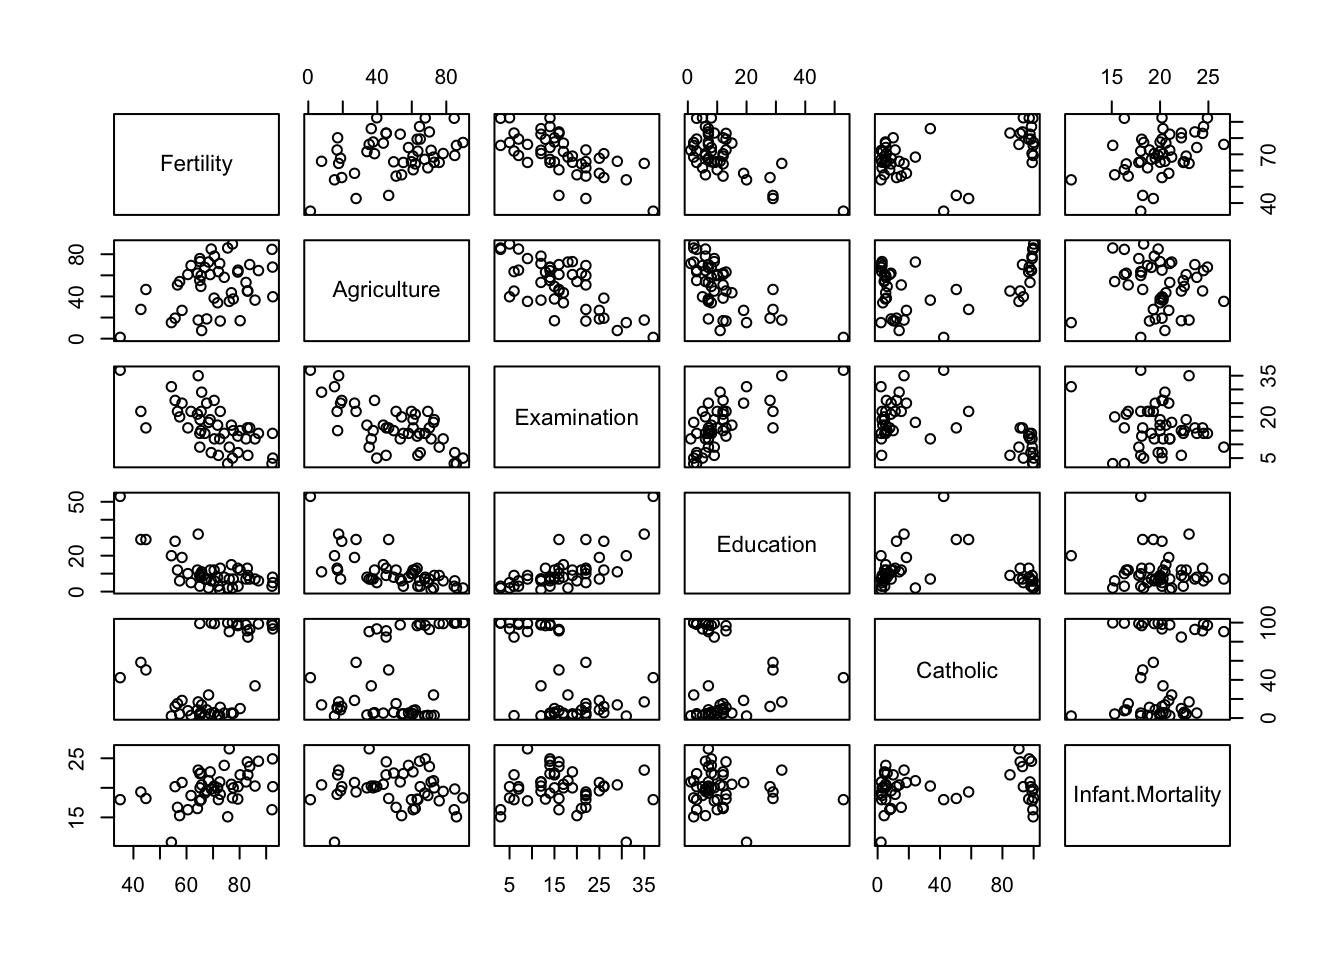
\includegraphics{01-intro_files/figure-latex/intro-plot-1.pdf}

Scatterplot of two dimensions

\begin{verbatim}
plot(swiss[,c("Education", "Fertility")])
# or
plot(swiss[4,1])
# or
plot(swiss$Education, swiss$Fertility)
# or
plot(swiss$Fertility ~ swiss$Education)
\end{verbatim}

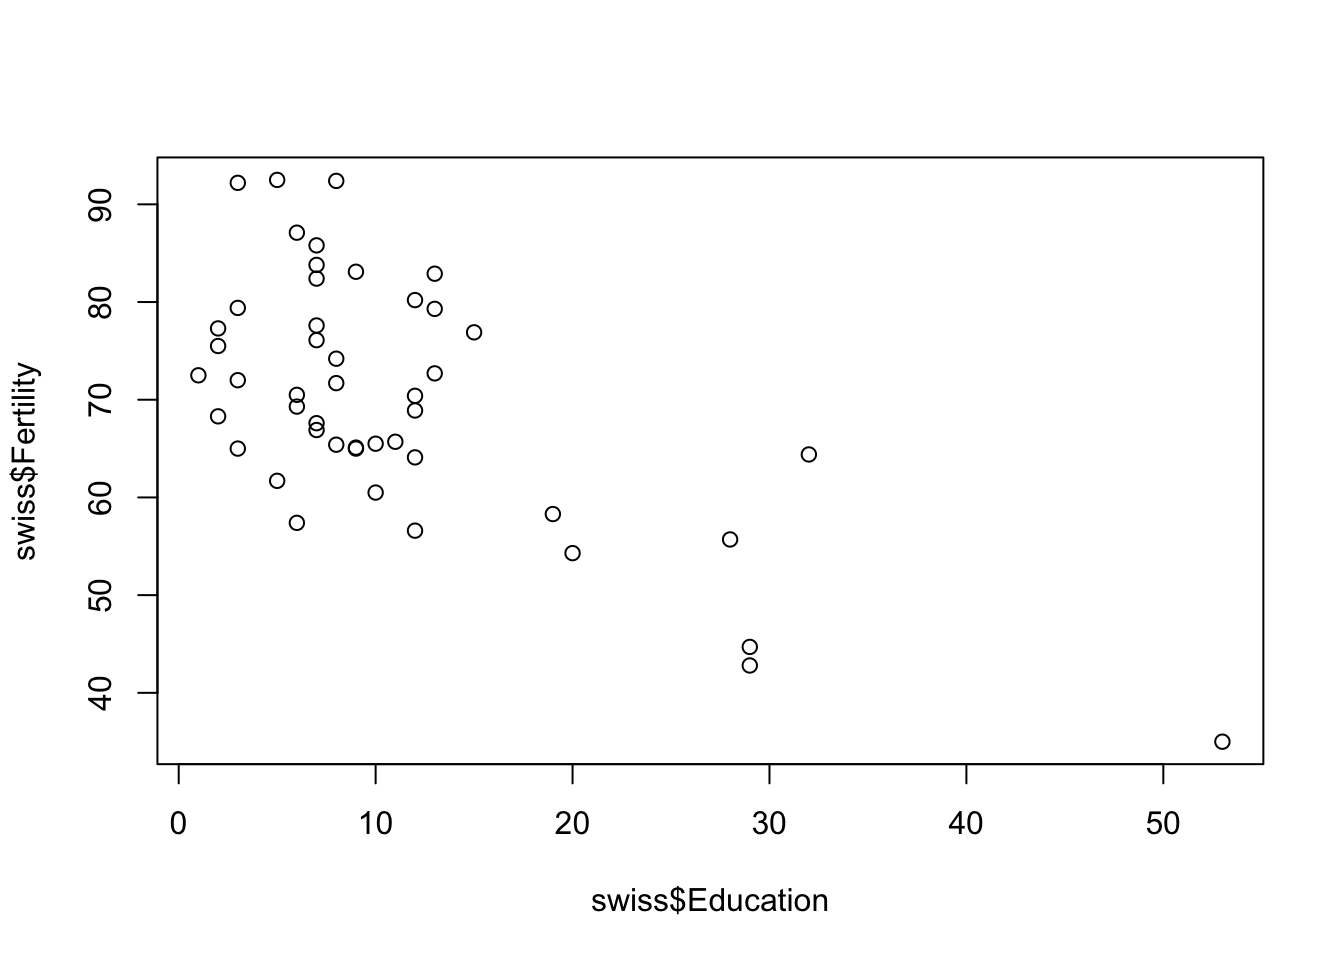
\includegraphics{01-intro_files/figure-latex/intro-cross-plot-1.pdf}

Smoothed Scatterplot of two dimensions

\begin{Shaded}
\begin{Highlighting}[]
\KeywordTok{smoothScatter}\NormalTok{(swiss$Fertility ~}\StringTok{ }\NormalTok{swiss$Examination)}
\end{Highlighting}
\end{Shaded}

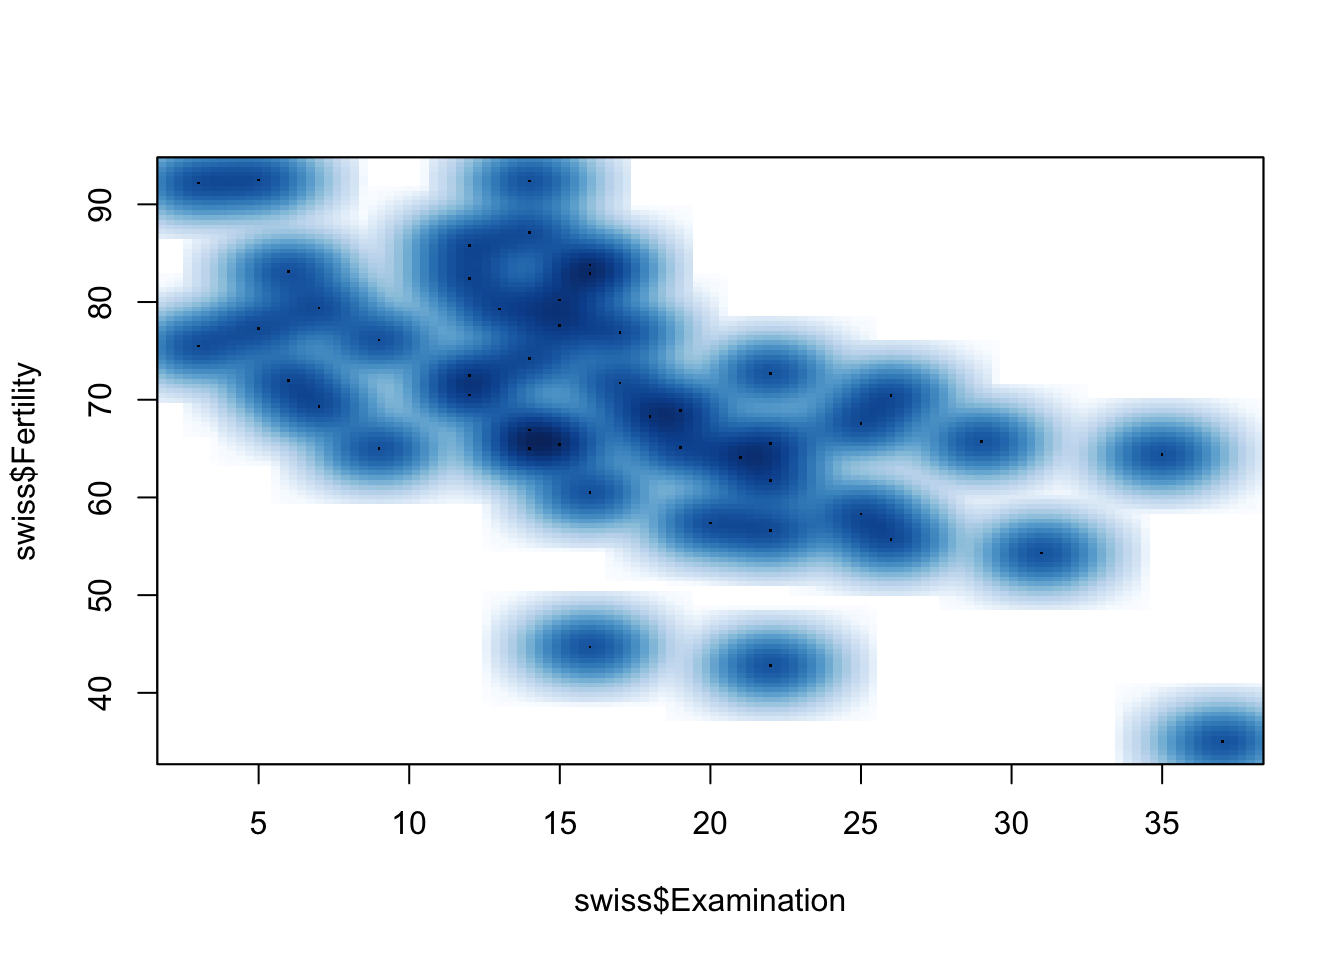
\includegraphics{01-intro_files/figure-latex/intro-smooth-scatter-1.pdf}

Scatterplot with a \texttt{loess} (locally weighted polynomial
regression)

\begin{Shaded}
\begin{Highlighting}[]
\KeywordTok{scatter.smooth}\NormalTok{(swiss$Fertility ~}\StringTok{ }\NormalTok{swiss$Agriculture)}
\end{Highlighting}
\end{Shaded}

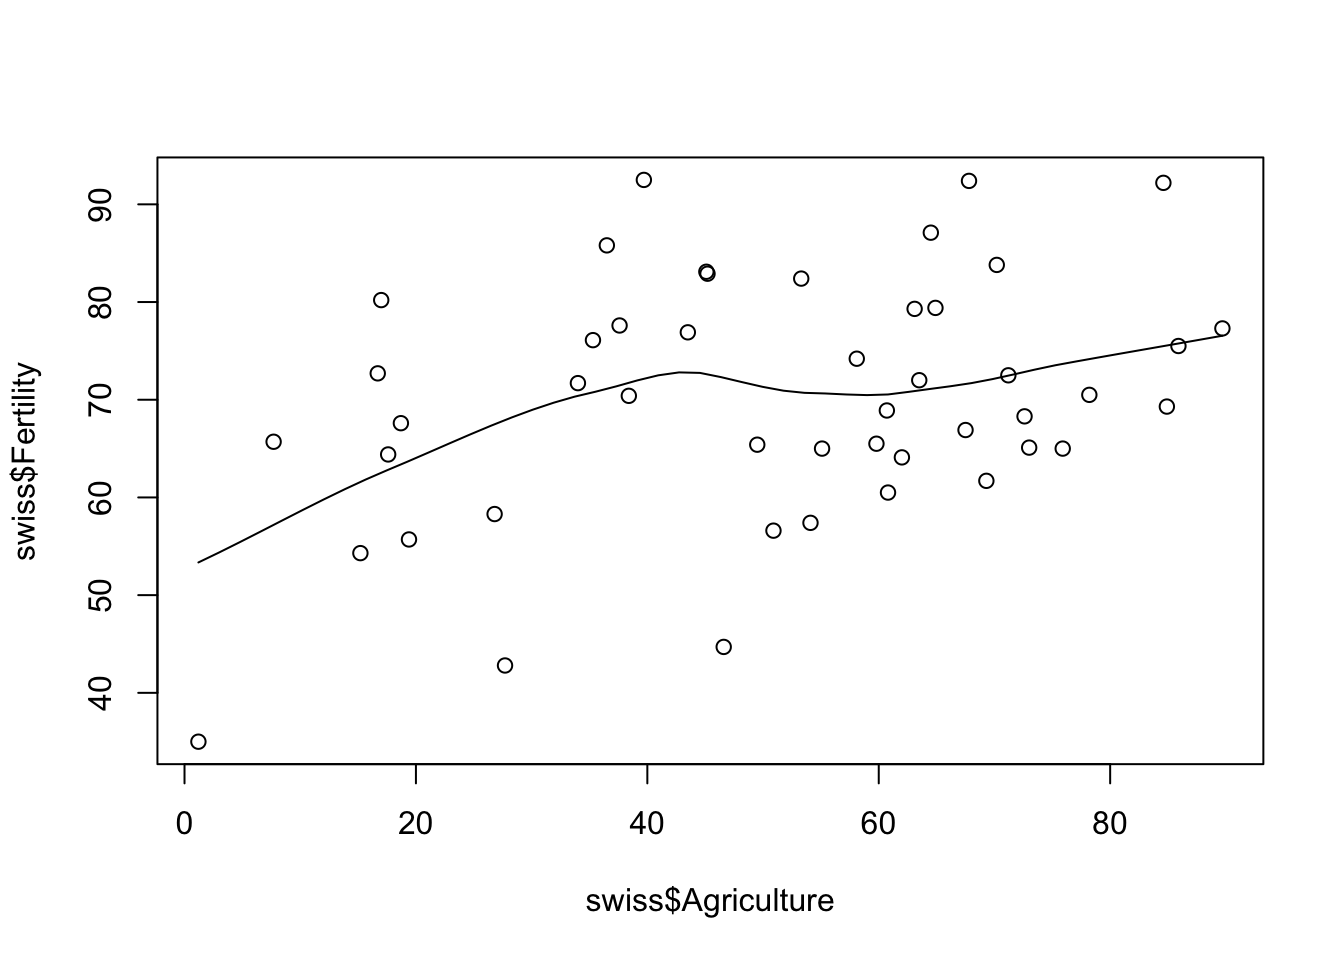
\includegraphics{01-intro_files/figure-latex/intro-smooth-1.pdf}

\subsection{Distribution plots}\label{distribution-plots}

Histograms:

\begin{Shaded}
\begin{Highlighting}[]
\KeywordTok{hist}\NormalTok{(swiss$Catholic)}
\end{Highlighting}
\end{Shaded}

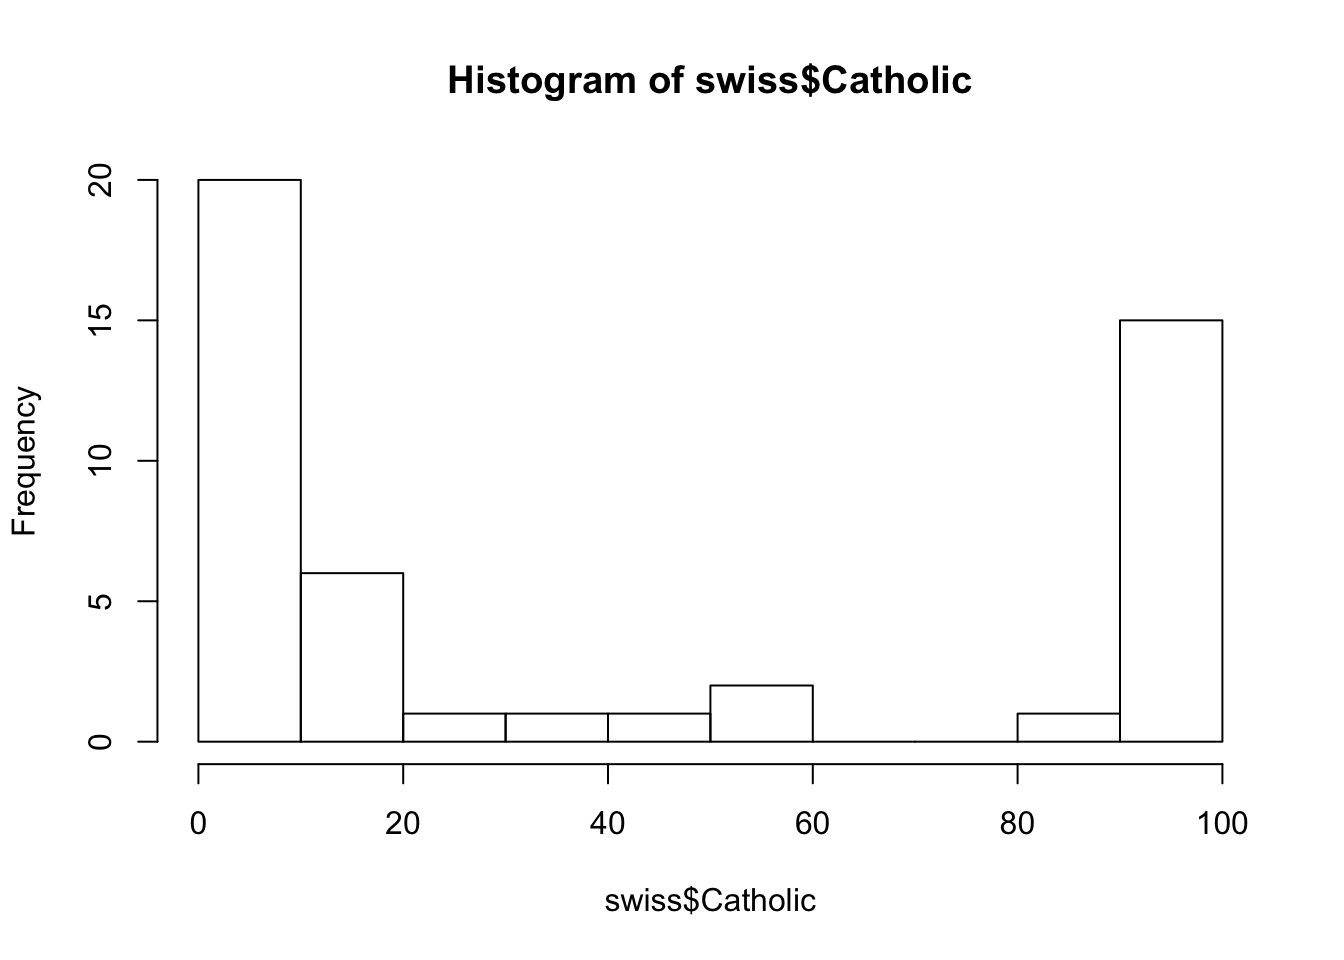
\includegraphics{01-intro_files/figure-latex/intro-hist-1.pdf}

Stem-and-Leaf Plots:

\begin{Shaded}
\begin{Highlighting}[]
\KeywordTok{stem}\NormalTok{(swiss$Fertility)}
\end{Highlighting}
\end{Shaded}

\begin{verbatim}
## 
##   The decimal point is 1 digit(s) to the right of the |
## 
##   3 | 5
##   4 | 35
##   5 | 46778
##   6 | 124455556678899
##   7 | 01223346677899
##   8 | 0233467
##   9 | 223
\end{verbatim}

Kernel density plot (and add a rug showing where observation occur):

\begin{Shaded}
\begin{Highlighting}[]
\KeywordTok{plot}\NormalTok{(}\KeywordTok{density}\NormalTok{(swiss$Fertility))}
\KeywordTok{rug}\NormalTok{(swiss$Fertility)}
\end{Highlighting}
\end{Shaded}

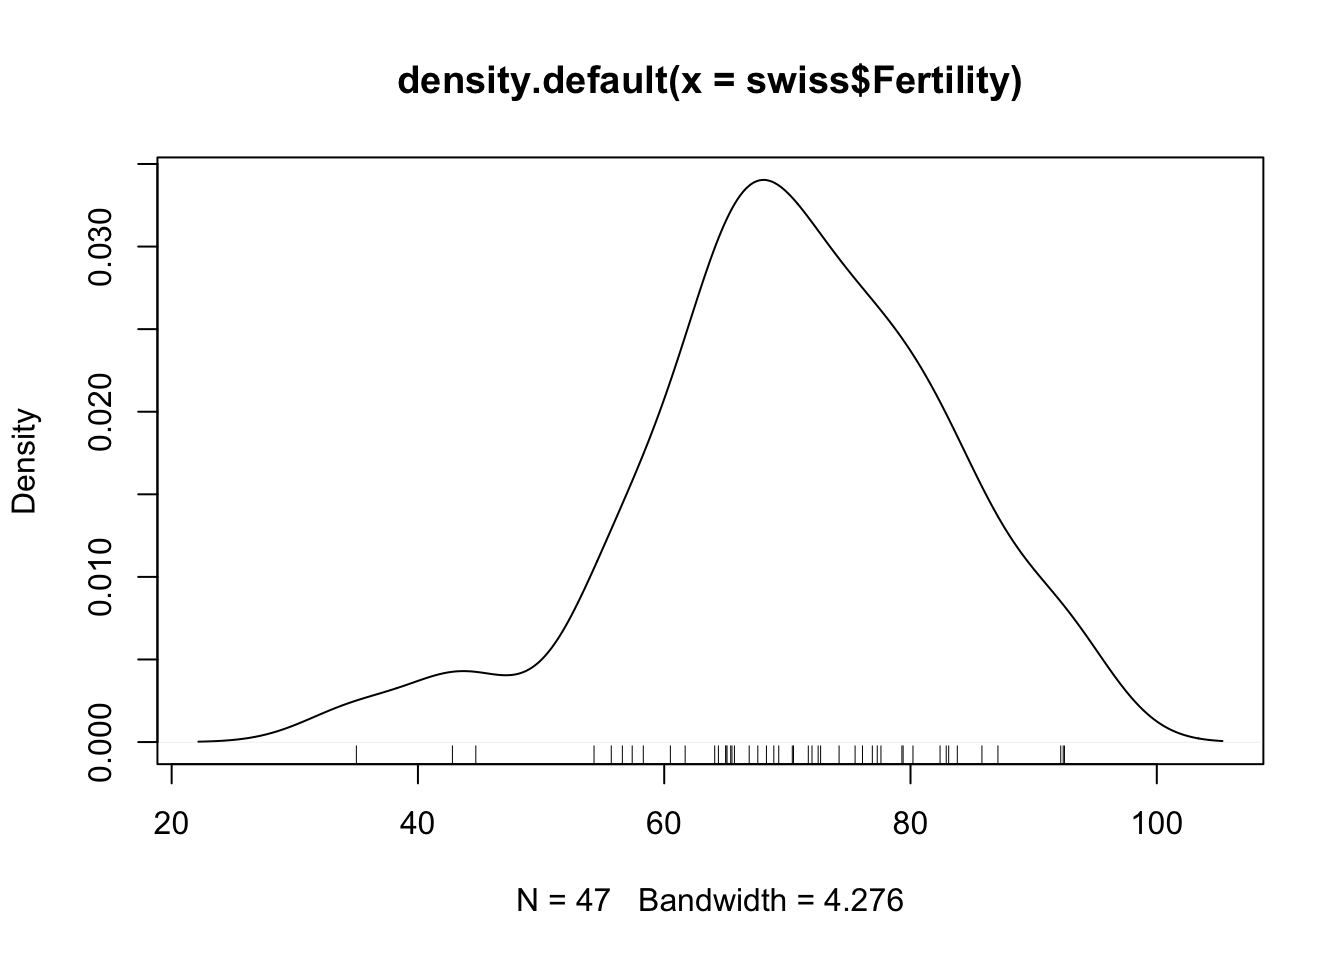
\includegraphics{01-intro_files/figure-latex/intro-rug-1.pdf}

Boxplots:

\begin{Shaded}
\begin{Highlighting}[]
\KeywordTok{boxplot}\NormalTok{(swiss)}
\end{Highlighting}
\end{Shaded}

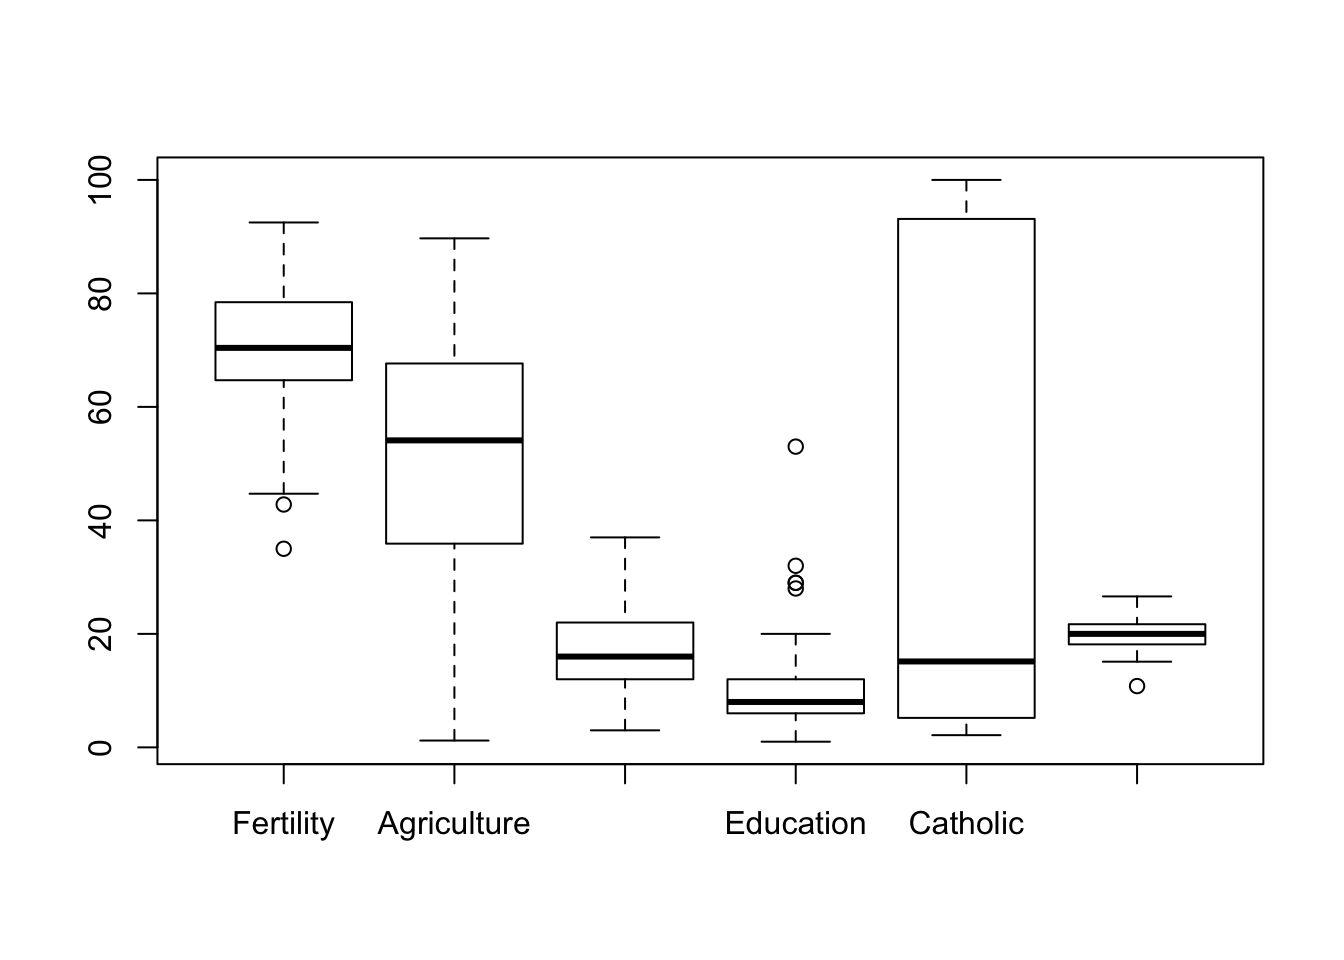
\includegraphics{01-intro_files/figure-latex/intro-boxplot-1.pdf}

\subsubsection{More complicated charts}\label{more-complicated-charts}

Conditioning plots:

\begin{Shaded}
\begin{Highlighting}[]
\KeywordTok{coplot}\NormalTok{(swiss$Fertility ~}\StringTok{ }\NormalTok{swiss$Examination |}\StringTok{ }\KeywordTok{as.factor}\NormalTok{(swiss$Catholic >}\StringTok{ }\DecValTok{50}\NormalTok{))}
\end{Highlighting}
\end{Shaded}

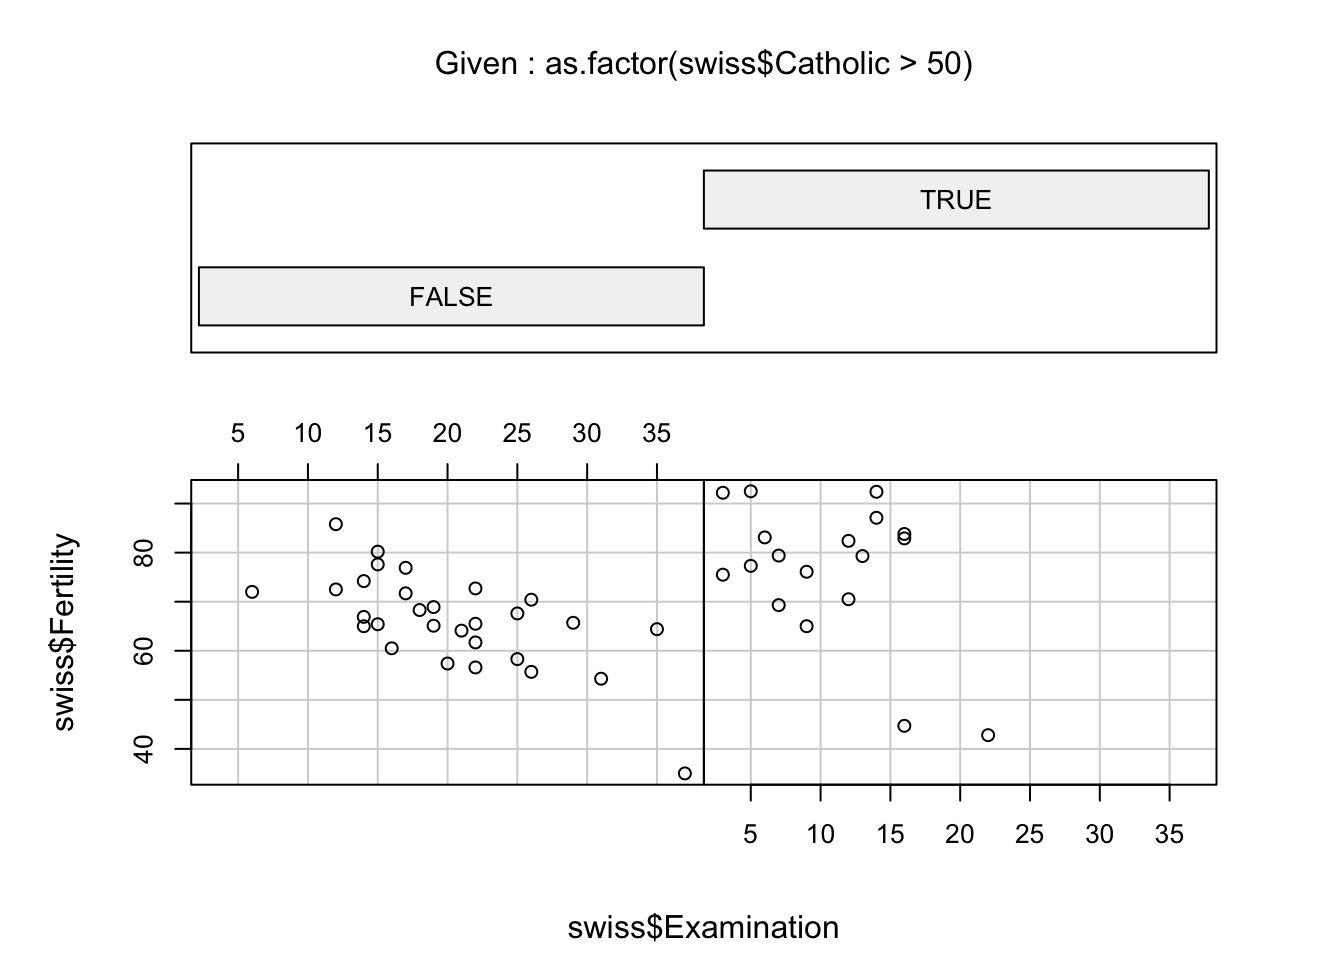
\includegraphics{01-intro_files/figure-latex/intro-coplot-1.pdf}

Star plots (half-star plots here):

\begin{Shaded}
\begin{Highlighting}[]
\KeywordTok{stars}\NormalTok{(swiss, }\DataTypeTok{key.loc =} \KeywordTok{c}\NormalTok{(}\DecValTok{15}\NormalTok{,}\DecValTok{1}\NormalTok{), }\DataTypeTok{flip.labels =} \OtherTok{FALSE}\NormalTok{, }\DataTypeTok{full =} \OtherTok{FALSE}\NormalTok{)}
\end{Highlighting}
\end{Shaded}

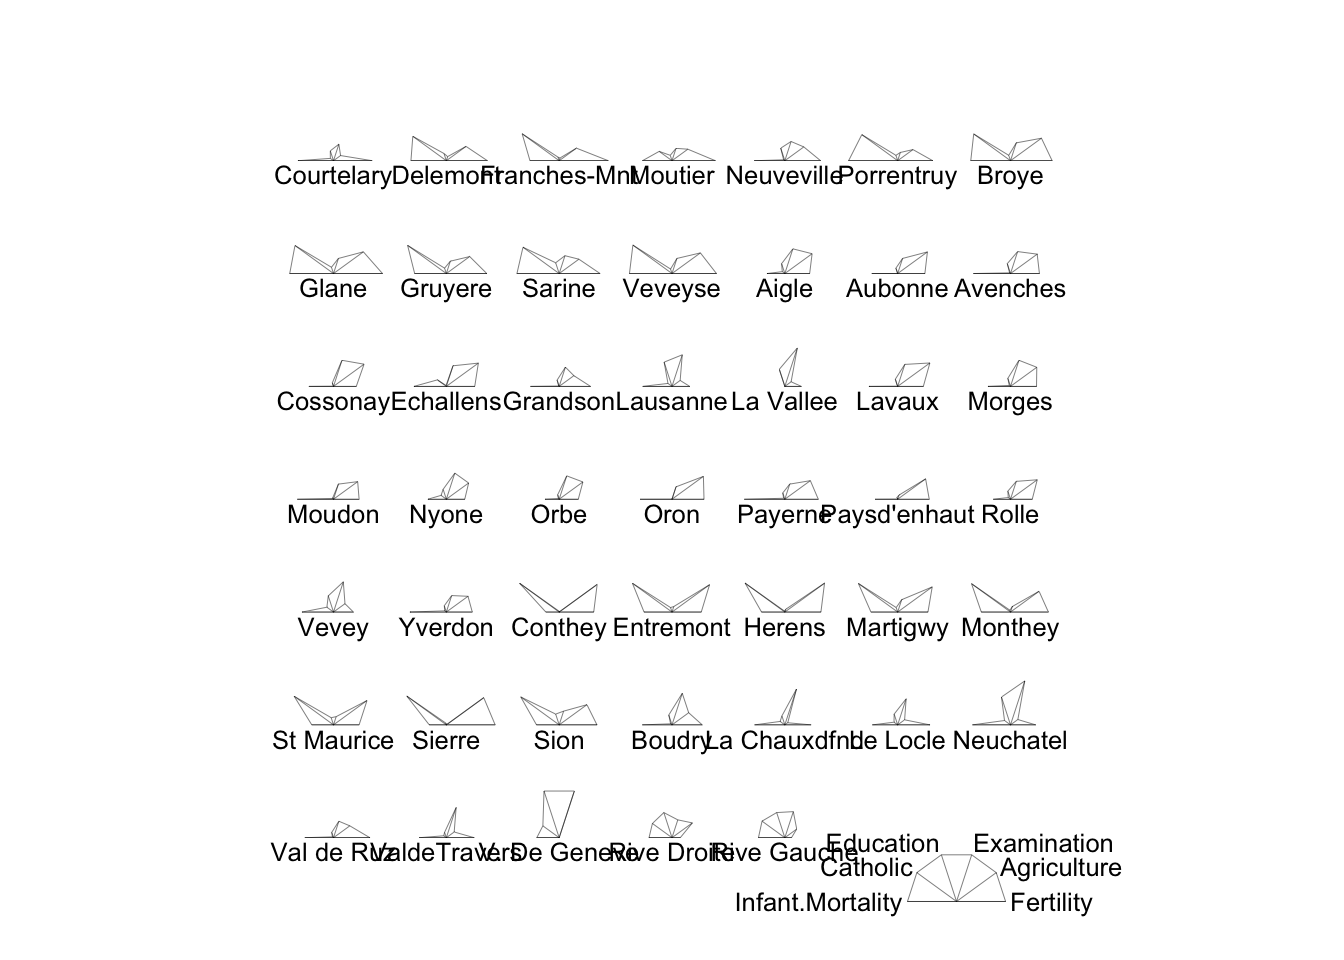
\includegraphics{01-intro_files/figure-latex/intro-star-1.pdf}

\section{Assignment}\label{assignment}

Create a new R Markdown file.

Choose a dataset from \texttt{datasets}
(\texttt{library(help\ =\ "datasets")} will show you a list) and create
5 charts in an R Markdown file from the example charts above. Run the
following command to see what else is available in the base R graphics
package:

\begin{verbatim}
demo(graphics)
\end{verbatim}

\hypertarget{read-data}{\chapter{Reading data}\label{read-data}}

The first step in analyzing data with R is reading data into it. This
lesson focuses on reading data, manipulating it with \texttt{dplyr} and
a few summary visualizations.

\section{Data Source:}\label{data-source}

The US Census Bureau has a large selection of data on the population of
the United States. The public-use micro surveys (PUMS) are available
from the following link:

\url{https://www.census.gov/programs-surveys/acs/data/pums.html}

We'll take a look at the 1-year American Community Survey results for
the state of Hawaii.

\href{https://www2.census.gov/programs-surveys/acs/data/pums/2015/1-Year/csv_phi.zip}{Hawaii
Population Records}

\href{https://www2.census.gov/programs-surveys/acs/tech_docs/pums/data_dict/PUMSDataDict15.txt}{The
data dictionary}

The specific file we are working with is the person record, so not every
variable in the data dictionary will be available. Only those under the
heading ``PERSON RECORD'' will be in the \texttt{csv\_phi.zip} file.

\section{\texorpdfstring{\texttt{read\_csv}}{read\_csv}}\label{read_csv}

To read in the downloaded file, we'll use the \texttt{readr} package,
which you can install by installing \texttt{tidyverse}.

\begin{Shaded}
\begin{Highlighting}[]
\KeywordTok{library}\NormalTok{(tidyverse)}
\NormalTok{pop_hi <-}\StringTok{ }\KeywordTok{read_csv}\NormalTok{(}\StringTok{"data/csv_phi.zip"}\NormalTok{)}
\NormalTok{pop_hi}
\end{Highlighting}
\end{Shaded}

\begin{verbatim}
## # A tibble: 14,124 x 284
##       RT SERIALNO SPORDER  PUMA    ST  ADJINC PWGTP  AGEP   CIT CITWP
##    <chr>    <int>   <chr> <chr> <int>   <int> <chr> <chr> <int> <int>
##  1     P       21      01 00303    15 1001264 00078    63     1    NA
##  2     P      158      01 00306    15 1001264 00056    54     1    NA
##  3     P      267      01 00100    15 1001264 00059    52     5    NA
##  4     P      267      02 00100    15 1001264 00071    56     5    NA
##  5     P      267      03 00100    15 1001264 00102    25     5    NA
##  6     P      267      04 00100    15 1001264 00155    22     5    NA
##  7     P      267      05 00100    15 1001264 00074    15     5    NA
##  8     P      351      01 00100    15 1001264 00307    32     4  2005
##  9     P      351      02 00100    15 1001264 00578    02     1    NA
## 10     P      470      01 00200    15 1001264 00041    79     1    NA
## # ... with 14,114 more rows, and 274 more variables: COW <int>,
## #   DDRS <int>, DEAR <int>, DEYE <int>, DOUT <int>, DPHY <int>,
## #   DRAT <int>, DRATX <int>, DREM <int>, ENG <int>, FER <int>, GCL <int>,
## #   GCM <int>, GCR <int>, HINS1 <int>, HINS2 <int>, HINS3 <int>,
## #   HINS4 <int>, HINS5 <int>, HINS6 <int>, HINS7 <int>, INTP <chr>,
## #   JWMNP <chr>, JWRIP <chr>, JWTR <chr>, LANX <int>, MAR <int>,
## #   MARHD <int>, MARHM <int>, MARHT <int>, MARHW <int>, MARHYP <int>,
## #   MIG <int>, MIL <int>, MLPA <int>, MLPB <int>, MLPCD <int>, MLPE <int>,
## #   MLPFG <int>, MLPH <int>, MLPI <int>, MLPJ <int>, MLPK <int>,
## #   NWAB <int>, NWAV <int>, NWLA <int>, NWLK <int>, NWRE <int>, OIP <chr>,
## #   PAP <chr>, RELP <chr>, RETP <chr>, SCH <int>, SCHG <chr>, SCHL <chr>,
## #   SEMP <chr>, SEX <int>, SSIP <chr>, SSP <chr>, WAGP <chr>, WKHP <chr>,
## #   WKL <int>, WKW <int>, WRK <int>, YOEP <int>, ANC <int>, ANC1P <chr>,
## #   ANC2P <chr>, DECADE <int>, DIS <int>, DRIVESP <int>, ESP <int>,
## #   ESR <int>, FHICOVP <int>, FOD1P <int>, FOD2P <int>, HICOV <int>,
## #   HISP <chr>, INDP <chr>, JWAP <chr>, JWDP <chr>, LANP <int>,
## #   MIGPUMA <chr>, MIGSP <chr>, MSP <int>, NAICSP <chr>, NATIVITY <int>,
## #   NOP <int>, OC <int>, OCCP <chr>, PAOC <int>, PERNP <chr>, PINCP <chr>,
## #   POBP <chr>, POVPIP <chr>, POWPUMA <chr>, POWSP <chr>, PRIVCOV <int>,
## #   PUBCOV <int>, QTRBIR <int>, ...
\end{verbatim}

\section{\texorpdfstring{\texttt{dplyr}}{dplyr}}\label{dplyr}

Using the data dictionary we can identify some interesting variables.

\begin{verbatim}
PERSON RECORD

RT      1   
    Record Type     
        P .Person Record

AGEP        2   
    Age
        00  .Under 1 year   
        01..99  .1 to 99 years (Top-coded***)

COW     1   
    Class of worker
        b .N/A (less than 16 years old/NILF who last
          .worked more than 5 years ago or never worked)
        1 .Employee of a private for-profit company or
          .business, or of an individual, for wages,
          .salary, or commissions
        2 .Employee of a private not-for-profit,
          .tax-exempt, or charitable organization
        3 .Local government employee (city, county, etc.)
        4 .State government employee
        5 .Federal government employee
        6 .Self-employed in own not incorporated
          .business, professional practice, or farm
        7 .Self-employed in own incorporated
          .business, professional practice or farm
        8 .Working without pay in family business or farm
        9 .Unemployed and last worked 5 years ago or earlier or never
                  .worked
        
SCHL        2   
    Educational attainment
        bb .N/A (less than 3 years old)
        01 .No schooling completed
        02 .Nursery school, preschool   
        03 .Kindergarten
        04 .Grade 1
        05 .Grade 2
        06 .Grade 3     
        07 .Grade 4
        08 .Grade 5
        09 .Grade 6
        10 .Grade 7     
        11 .Grade 8  
        12 .Grade 9
        13 .Grade 10
        14 .Grade 11        
        15 .12th grade - no diploma   
        16 .Regular high school diploma
        17 .GED or alternative credential
        18 .Some college, but less than 1 year
        19 .1 or more years of college credit, no degree
        20 .Associate's degree      
        21 .Bachelor's degree
        22 .Master's degree
        23 .Professional degree beyond a bachelor's degree
        24 .Doctorate degree
        
WAGP        6   
    Wages or salary income past 12 months
        bbbbbb      .N/A (less than 15 years old)
        000000      .None
        000001..999999  .$1 to 999999 (Rounded and top-coded)

Note: Use ADJINC to adjust WAGP to constant dollars.


WKHP        2   
    Usual hours worked per week past 12 months
        bb   .N/A (less than 16 years old/did not work 
             .during the past 12 months)
        01..98   .1 to 98 usual hours
        99   .99 or more usual hours
        
WKW     1   
    Weeks worked during past 12 months
        b .N/A (less than 16 years old/did not work 
          .during the past 12 months)
        1 .50 to 52 weeks worked during past 12 months
        2 .48 to 49 weeks worked during past 12 months
        3 .40 to 47 weeks worked during past 12 months
        4 .27 to 39 weeks worked during past 12 months
        5 .14 to 26 weeks worked during past 12 months 
        6 .less than 14 weeks worked during past 12 months
        
ESR     1   
    Employment status recode
        b .N/A (less than 16 years old)
        1 .Civilian employed, at work
        2 .Civilian employed, with a job but not at work
        3 .Unemployed
        4 .Armed forces, at work
        5 .Armed forces, with a job but not at work
        6 .Not in labor force
        
PERNP       7   
    Total person's earnings
        bbbbbbb         .N/A (less than 15 years old)
        0000000         .No earnings
        -010000         .Loss of $10000 or more (Rounded & bottom-coded 
                        .components) 
        -000001..-009999    .Loss $1 to $9999 (Rounded components)
        0000001         .$1 or break even
        0000002..9999999    .$2 to $9999999 (Rounded & top-coded components)
        
Note: Use ADJINC to adjust PERNP to constant dollars.

PINCP       7   
    Total person's income (signed)
        bbbbbbb         .N/A (less than 15 years old)
        0000000         .None
        -019999         .Loss of $19999 or more (Rounded & bottom-coded 
                        .components) 
        -000001..-019998    .Loss $1 to $19998 (Rounded components)
        0000001         .$1 or break even
        0000002..9999999    .$2 to $9999999 (Rounded & top-coded components)
            
Note: Use ADJINC to adjust PINCP to constant dollars.
\end{verbatim}

Let's focus on employed civilians (ESR either 1 or 2) working full time
(WKHP \textgreater{} 32) for close to the entire year (WKW either 1 or
2).

\begin{Shaded}
\begin{Highlighting}[]
\NormalTok{pop_hi <-}\StringTok{ }\NormalTok{pop_hi %>%}
\StringTok{  }\KeywordTok{filter}\NormalTok{(}
    \NormalTok{ESR %in%}\StringTok{ }\KeywordTok{c}\NormalTok{(}\DecValTok{1}\NormalTok{, }\DecValTok{2}\NormalTok{),}
    \KeywordTok{as.numeric}\NormalTok{(WKHP) >}\StringTok{ }\DecValTok{32}\NormalTok{,}
    \NormalTok{WKW %in%}\StringTok{ }\KeywordTok{c}\NormalTok{(}\DecValTok{1}\NormalTok{, }\DecValTok{2}\NormalTok{)}
  \NormalTok{)}
\end{Highlighting}
\end{Shaded}

If you are unsure if a column that you want to treat as numeric contains
letters, you can run the following command to get a list of the values
containing letters:

\begin{Shaded}
\begin{Highlighting}[]
\KeywordTok{grep}\NormalTok{(}\StringTok{"[[:alpha:]]"}\NormalTok{, pop_hi$WKHP, }\DataTypeTok{value =} \OtherTok{TRUE}\NormalTok{)}
\end{Highlighting}
\end{Shaded}

\begin{verbatim}
## character(0)
\end{verbatim}

We can use two functions to add new columns (or change existing ones).

\begin{enumerate}
\def\labelenumi{\arabic{enumi}.}
\tightlist
\item
  \texttt{mutate()} adds columns and keeps the previous columns
\item
  \texttt{transmute()} adds columns and removes the previous columns
\end{enumerate}

This time we want to drop the columns we don't mention.

\begin{Shaded}
\begin{Highlighting}[]
\NormalTok{pop_hi <-}\StringTok{ }\NormalTok{pop_hi %>%}
\StringTok{  }\KeywordTok{transmute}\NormalTok{(}
    \DataTypeTok{age =} \KeywordTok{as.numeric}\NormalTok{(AGEP),}
    \DataTypeTok{worker_class =} \KeywordTok{factor}\NormalTok{(COW, }\DataTypeTok{labels =} \KeywordTok{c}\NormalTok{(}
      \StringTok{"for-profit"}\NormalTok{,}
      \StringTok{"not-for-profit"}\NormalTok{,}
      \StringTok{"local government"}\NormalTok{,}
      \StringTok{"state government"}\NormalTok{,}
      \StringTok{"federal government"}\NormalTok{,}
      \StringTok{"self-employed not incorporated"}\NormalTok{,}
      \StringTok{"self-employed incorporated"}\NormalTok{,}
      \StringTok{"family business no pay"}
    \NormalTok{)),}
    \DataTypeTok{school =} \NormalTok{SCHL,}
    \DataTypeTok{wages =} \KeywordTok{as.numeric}\NormalTok{(WAGP),}
    \DataTypeTok{top_coded_wages =} \NormalTok{WAGP ==}\StringTok{ }\DecValTok{999999}
\NormalTok{)}
\end{Highlighting}
\end{Shaded}

Creating a custom factor variable for educational attainment:

\begin{Shaded}
\begin{Highlighting}[]
\NormalTok{education_levels <-}\StringTok{ }\KeywordTok{c}\NormalTok{(}\StringTok{"less than HS"}\NormalTok{, }\StringTok{"HS"}\NormalTok{, }\StringTok{"associates"}\NormalTok{, }\StringTok{"bachelors"}\NormalTok{, }\StringTok{"masters"}\NormalTok{, }\StringTok{"doctorate"}\NormalTok{)}

\NormalTok{pop_hi$education <-}\StringTok{ }\OtherTok{NA}
\NormalTok{pop_hi[pop_hi$school <}\StringTok{ }\DecValTok{16}\NormalTok{,]$education <-}\StringTok{ "less than HS"}
\NormalTok{pop_hi[pop_hi$school >}\StringTok{ }\DecValTok{16} \NormalTok{&}\StringTok{ }\NormalTok{pop_hi$school <}\StringTok{ }\DecValTok{20}\NormalTok{,]$education <-}\StringTok{ "HS"}
\NormalTok{pop_hi[pop_hi$school ==}\StringTok{ }\DecValTok{20}\NormalTok{,]$education <-}\StringTok{ "associates"}
\NormalTok{pop_hi[pop_hi$school ==}\StringTok{ }\DecValTok{21}\NormalTok{,]$education <-}\StringTok{ "bachelors"}
\NormalTok{pop_hi[pop_hi$school %in%}\StringTok{ }\KeywordTok{c}\NormalTok{(}\DecValTok{22}\NormalTok{, }\DecValTok{23}\NormalTok{),]$education <-}\StringTok{ "masters"}
\NormalTok{pop_hi[pop_hi$school ==}\StringTok{ }\DecValTok{24}\NormalTok{,]$education <-}\StringTok{ "doctorate"}

\NormalTok{pop_hi <-}\StringTok{ }\NormalTok{pop_hi %>%}
\StringTok{  }\KeywordTok{mutate}\NormalTok{(}\DataTypeTok{education =} \KeywordTok{factor}\NormalTok{(education, }\DataTypeTok{levels =} \NormalTok{education_levels))}
\end{Highlighting}
\end{Shaded}

\section{\texorpdfstring{First Look at
\texttt{ggplot2}}{First Look at ggplot2}}\label{first-look-at-ggplot2}

See the \href{ggplot2.tidyverse.org/reference/}{ggplot2 documentation}
for details and inspiration.

\begin{Shaded}
\begin{Highlighting}[]
\KeywordTok{ggplot}\NormalTok{(pop_hi, }\KeywordTok{aes}\NormalTok{(age, wages)) +}
\StringTok{  }\KeywordTok{geom_point}\NormalTok{()}
\end{Highlighting}
\end{Shaded}

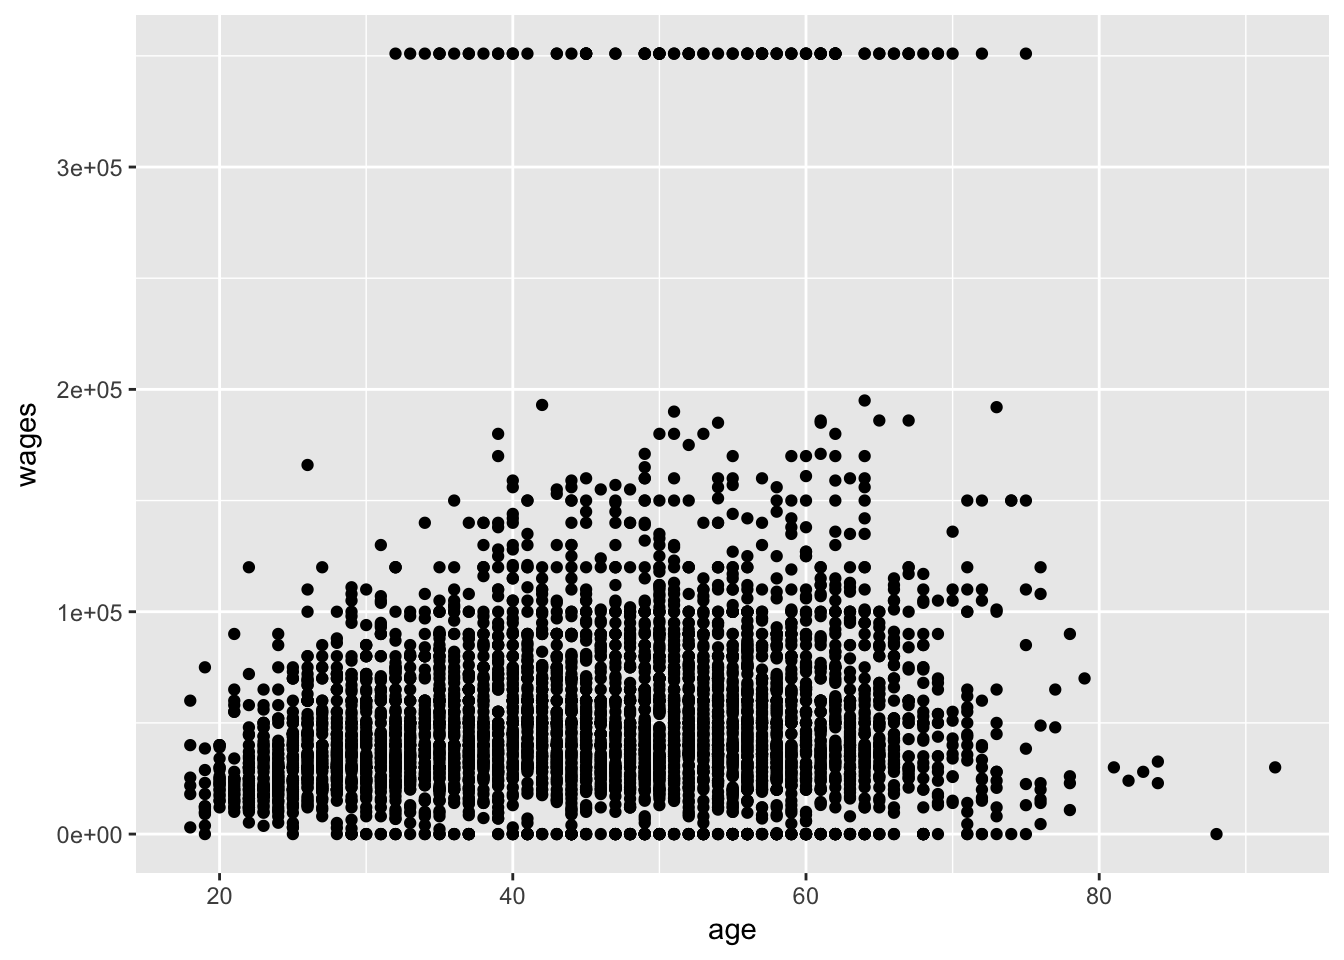
\includegraphics{02-read-data_files/figure-latex/read-point-1.pdf}

Income has a skewed distribution, so it is often presented/analyzed in
logs. Here's how to modify the above chart to display income in logs:

\begin{Shaded}
\begin{Highlighting}[]
\NormalTok{pop_hi <-}\StringTok{ }\NormalTok{pop_hi %>%}
\StringTok{  }\KeywordTok{mutate}\NormalTok{(}\DataTypeTok{log_safe_wages =} \KeywordTok{ifelse}\NormalTok{(wages ==}\StringTok{ }\DecValTok{0}\NormalTok{, }\DecValTok{1}\NormalTok{, wages))}
\NormalTok{pop_hi %>%}
\StringTok{  }\KeywordTok{ggplot}\NormalTok{(}\KeywordTok{aes}\NormalTok{(age, log_safe_wages)) +}
\StringTok{  }\KeywordTok{geom_point}\NormalTok{() +}
\StringTok{  }\KeywordTok{scale_y_log10}\NormalTok{()}
\end{Highlighting}
\end{Shaded}

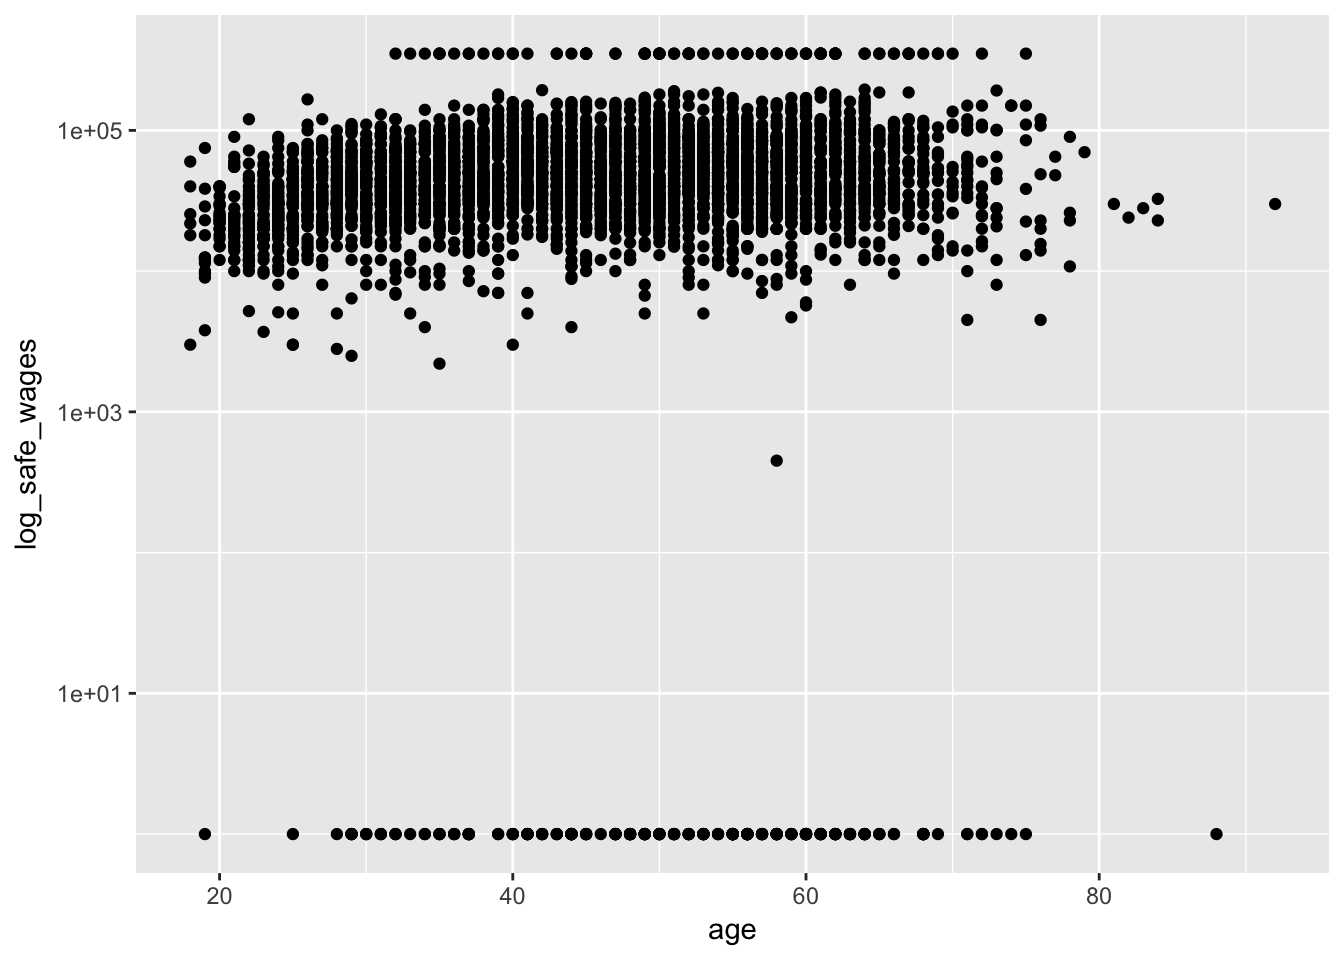
\includegraphics{02-read-data_files/figure-latex/read-scale-1.pdf}

\section{Heatmaps}\label{heatmaps}

Heatmaps allow you to get a sense of the concetration of observations in
regions where there are many overlapping points:

\begin{Shaded}
\begin{Highlighting}[]
\KeywordTok{ggplot}\NormalTok{(pop_hi, }\KeywordTok{aes}\NormalTok{(age, log_safe_wages)) +}
\StringTok{  }\KeywordTok{geom_bin2d}\NormalTok{() +}
\StringTok{  }\KeywordTok{scale_y_log10}\NormalTok{()}
\end{Highlighting}
\end{Shaded}

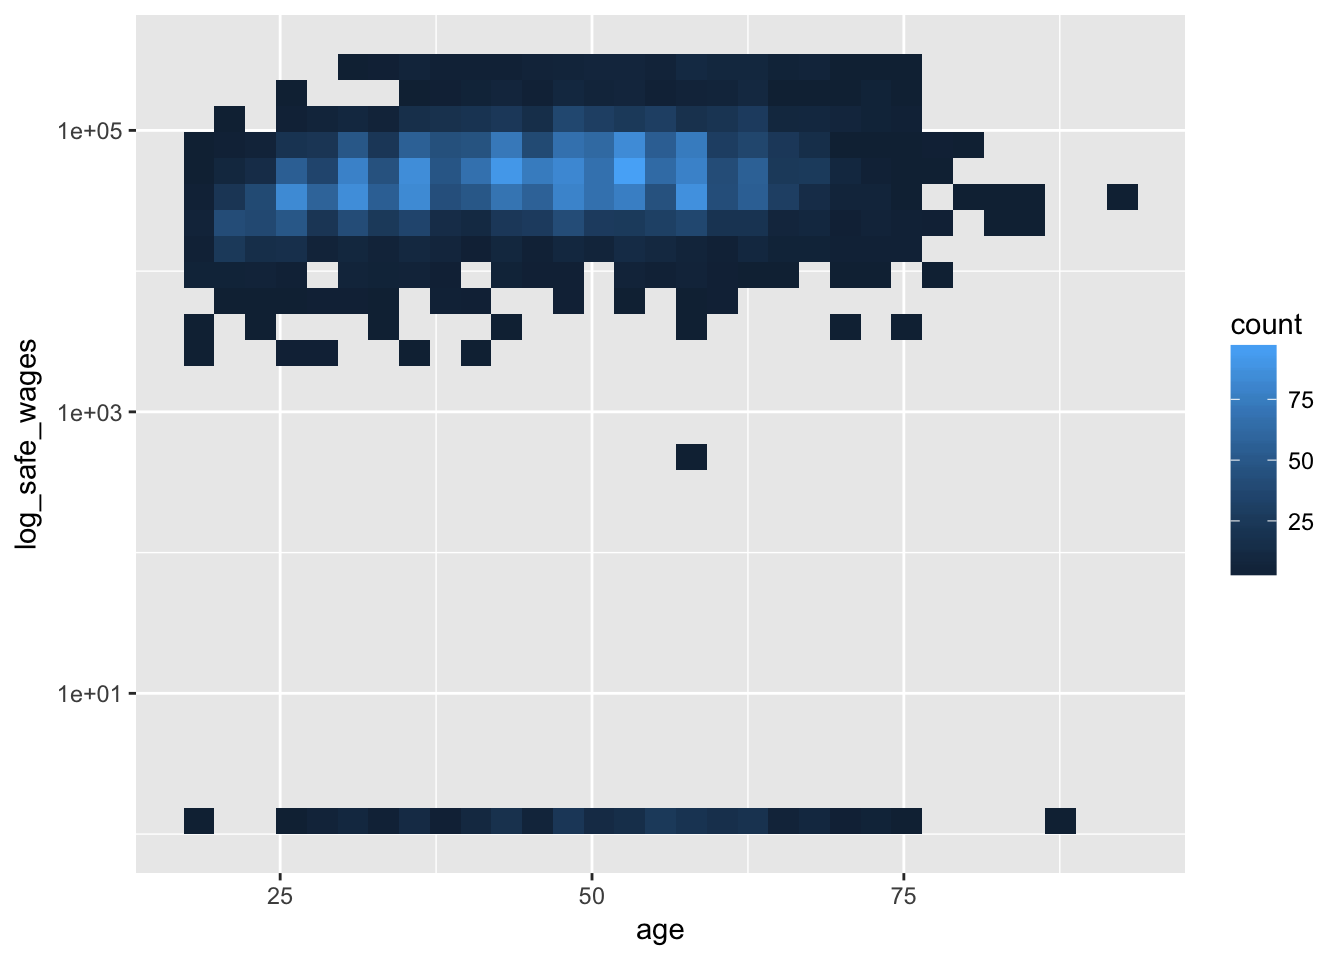
\includegraphics{02-read-data_files/figure-latex/read-bin2d-1.pdf}

\section{Hexbins}\label{hexbins}

Hexbins use hexagons instead of squares, which helps avoid the
rectangular sections in heatmaps that may misrepresent your data.

You will need to install the \texttt{hexbin} package.

\begin{verbatim}
install.packages("hexbin")
\end{verbatim}

\begin{Shaded}
\begin{Highlighting}[]
\NormalTok{pop_hi %>%}
\StringTok{  }\KeywordTok{filter}\NormalTok{(wages >}\StringTok{ }\DecValTok{10000}\NormalTok{, wages <}\StringTok{ }\DecValTok{300000}\NormalTok{) %>%}
\StringTok{  }\KeywordTok{ggplot}\NormalTok{(}\KeywordTok{aes}\NormalTok{(age, wages)) +}
\StringTok{  }\KeywordTok{geom_hex}\NormalTok{() +}\StringTok{ }
\StringTok{  }\KeywordTok{scale_x_log10}\NormalTok{()}
\end{Highlighting}
\end{Shaded}

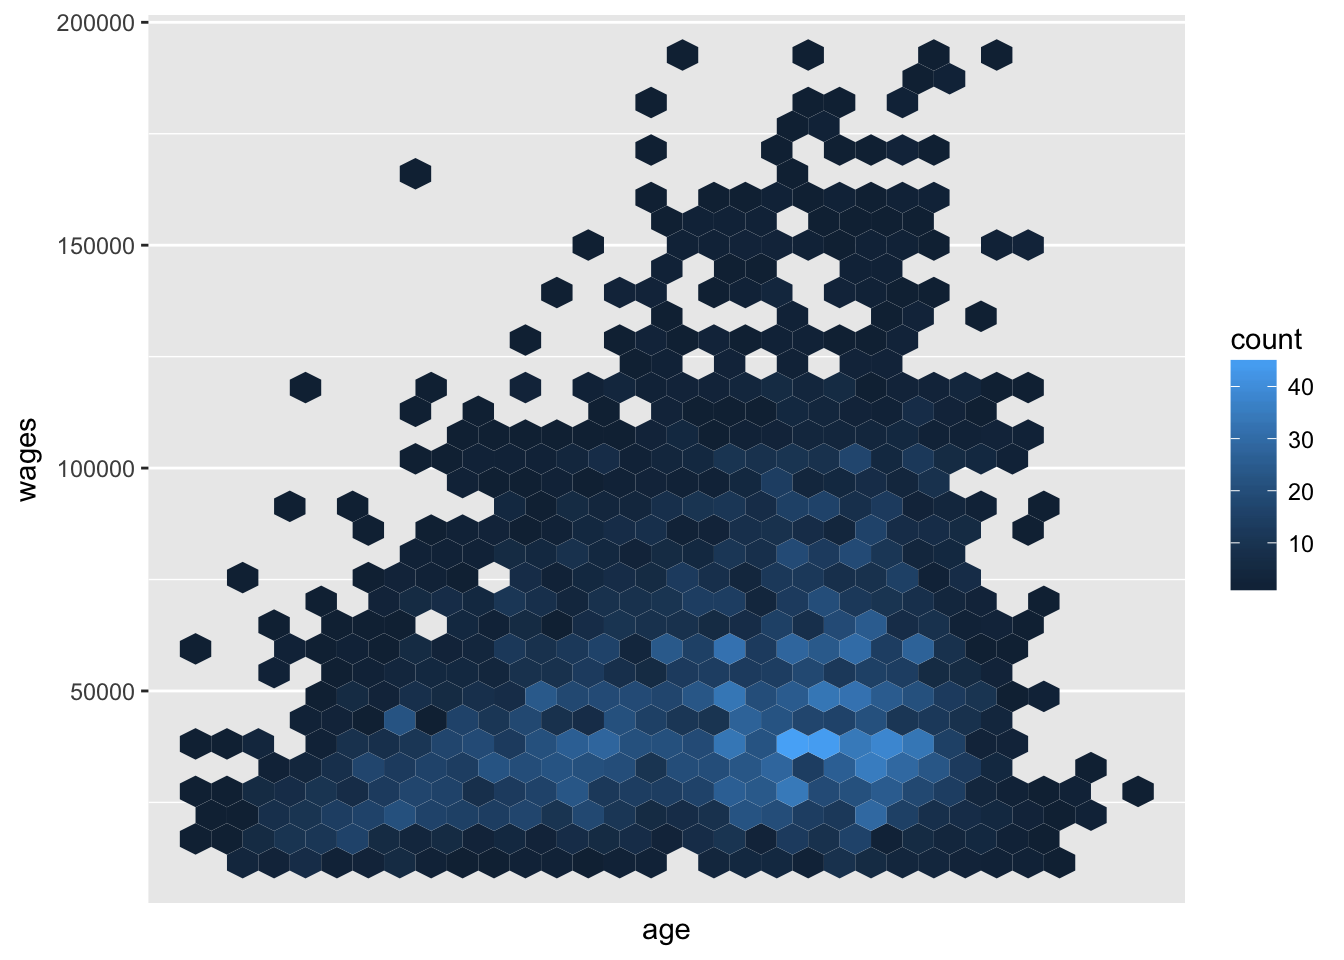
\includegraphics{02-read-data_files/figure-latex/read-hex-1.pdf}

Here we can see that inequality in wages for workers increases with age.

\section{Other topics from this
dataset}\label{other-topics-from-this-dataset}

This dataset includes information on the majors for degree holders and
the industry codes. You could use that additional information to ask how
well targeted majors are to particular industries and how incomes vary
across choice of major. Because of the size of the data in the Hawaii
sample, it would be better to ask some of these questions at the
national level.

Go to the
\href{https://www.census.gov/programs-surveys/acs/technical-documentation/pums/documentation.2015.html}{ACS
PUMS documentation page} for more information.

\section{Assignment}\label{assignment-1}

Choose another pair of variables from the data dictionary and visualize
them with a scatterplot, a heatmap, and a hexbin plot.

\hypertarget{facets-and-bubbles}{\chapter{Facets, Bubbles, and
Transparency}\label{facets-and-bubbles}}

\section{Data}\label{data}

For this session, we'll explore the Hawaii Tourism Authority (HTA)
\href{http://www.hawaiitourismauthority.org/research/research/infrastructure-research/}{Air
Seat Projection}. I'll be working with the
\href{http://www.hawaiitourismauthority.org/default/assets/File/2017\%20Air\%20Seat\%20Forecast\%20rev\%200617.xls}{Air
Seat Projection for 2017 (revised 06/17)}. Feel free to download the
latest available.

\subsection{Importing non-standard Excel
files}\label{importing-non-standard-excel-files}

The first steps in preparing a non-standard Excel file are (1) identify
how many rows to skip and (2) provide column names if the column names
are not neatly contained in a single row. You may also want to set the
\texttt{range} if there is metadata at the end of the table you are
importing. \texttt{range} overrides any \texttt{skip} setting, so we
wont have to specify the number of rows to skip.

\begin{Shaded}
\begin{Highlighting}[]
\KeywordTok{library}\NormalTok{(tidyverse)}
\KeywordTok{library}\NormalTok{(readxl)}
\end{Highlighting}
\end{Shaded}

\begin{Shaded}
\begin{Highlighting}[]
\NormalTok{seats <-}\StringTok{ }\KeywordTok{read_excel}\NormalTok{(}\StringTok{"data/2017 Air Seat Forecast rev 0617.xls"}\NormalTok{, }\DataTypeTok{col_names =} \KeywordTok{c}\NormalTok{(}
  \StringTok{"dep_city"}\NormalTok{, }
  \StringTok{"seats2017Q1"}\NormalTok{, }\StringTok{"seats2017Q2"}\NormalTok{, }\StringTok{"seats2017Q3"}\NormalTok{, }\StringTok{"seats2017Q4"}\NormalTok{, }\StringTok{"seats2017"}\NormalTok{, }
  \StringTok{"seats2016Q1"}\NormalTok{, }\StringTok{"seats2016Q2"}\NormalTok{, }\StringTok{"seats2016Q3"}\NormalTok{, }\StringTok{"seats2016Q4"}\NormalTok{, }\StringTok{"seats2016"}\NormalTok{,}
  \StringTok{"seatschangeQ1"}\NormalTok{, }\StringTok{"seatschangeQ2"}\NormalTok{, }\StringTok{"seatschangeQ3"}\NormalTok{, }\StringTok{"seatschangeQ4"}\NormalTok{, }\StringTok{"seatschange"}
\NormalTok{), }\DataTypeTok{range =} \StringTok{"A5:P78"}\NormalTok{)}
\NormalTok{seats}
\end{Highlighting}
\end{Shaded}

\begin{verbatim}
## # A tibble: 74 x 16
##     dep_city seats2017Q1 seats2017Q2 seats2017Q3 seats2017Q4 seats2017
##        <chr>       <dbl>       <dbl>       <dbl>       <dbl>     <dbl>
##  1     TOTAL     2987920     3016376     3168233     3050112  12222641
##  2 SCHEDULED     2966915     2996155     3140998     3029794  12133862
##  3  CHARTERS       21005       20221       27235       20318     88779
##  4      <NA>          NA          NA          NA          NA        NA
##  5  US TOTAL     1996549     2108969     2215424     2071513   8392455
##  6 SCHEDULED     1978616     2091981     2200195     2055171   8325963
##  7  CHARTERS       17933       16988       15229       16342     66492
##  8      <NA>          NA          NA          NA          NA        NA
##  9   US WEST     1717254     1837080     1943653     1817441   7315428
## 10 Anchorage       25758       15105       13674       17013     71550
## # ... with 64 more rows, and 10 more variables: seats2016Q1 <dbl>,
## #   seats2016Q2 <dbl>, seats2016Q3 <dbl>, seats2016Q4 <dbl>,
## #   seats2016 <dbl>, seatschangeQ1 <dbl>, seatschangeQ2 <chr>,
## #   seatschangeQ3 <chr>, seatschangeQ4 <dbl>, seatschange <dbl>
\end{verbatim}

Let's add a region identifier

\begin{Shaded}
\begin{Highlighting}[]
\NormalTok{us_west_range <-}\StringTok{ }\DecValTok{10}\NormalTok{:}\DecValTok{23}
\NormalTok{us_east_range <-}\StringTok{ }\DecValTok{26}\NormalTok{:}\DecValTok{33}
\NormalTok{japan_range <-}\StringTok{ }\DecValTok{40}\NormalTok{:}\DecValTok{45}
\NormalTok{canada_range <-}\StringTok{ }\DecValTok{48}\NormalTok{:}\DecValTok{52}
\NormalTok{other_asia_range <-}\DecValTok{55}\NormalTok{:}\DecValTok{58}
\NormalTok{oceania_range <-}\StringTok{ }\DecValTok{61}\NormalTok{:}\DecValTok{64}
\NormalTok{other_range <-}\StringTok{ }\DecValTok{67}\NormalTok{:}\DecValTok{74}

\NormalTok{seats$region <-}\StringTok{ }\OtherTok{NA}
\NormalTok{seats[us_west_range,]$region <-}\StringTok{ "US West"}
\NormalTok{seats[us_east_range,]$region <-}\StringTok{ "US East"}
\NormalTok{seats[japan_range,]$region <-}\StringTok{ "Japan"}
\NormalTok{seats[canada_range,]$region <-}\StringTok{ "Canada"}
\NormalTok{seats[other_asia_range,]$region <-}\StringTok{ "Other Asia"}
\NormalTok{seats[oceania_range,]$region <-}\StringTok{ "Oceania"}
\NormalTok{seats[other_range,]$region <-}\StringTok{ "Other"}

\NormalTok{seats <-}\StringTok{ }\NormalTok{seats %>%}
\StringTok{  }\KeywordTok{filter}\NormalTok{(!}\KeywordTok{is.na}\NormalTok{(region))}
\NormalTok{seats}
\end{Highlighting}
\end{Shaded}

\begin{verbatim}
## # A tibble: 49 x 17
##          dep_city seats2017Q1 seats2017Q2 seats2017Q3 seats2017Q4
##             <chr>       <dbl>       <dbl>       <dbl>       <dbl>
##  1      Anchorage       25758       15105       13674       17013
##  2     Bellingham       10198         318          NA        6519
##  3         Denver       55803       51654       52585       43290
##  4      Las Vegas       70514       74322       75839       75415
##  5    Los Angeles      548935      647498      715338      647703
##  6        Oakland       84571      104810      116015       90703
##  7        Phoenix      113046      115125      125348      108863
##  8       Portland       90207       71068       65997       81673
##  9     Sacramento       37620       38318       38456       38456
## 10 Salt Lake City       26370       23751       22968       28322
## # ... with 39 more rows, and 12 more variables: seats2017 <dbl>,
## #   seats2016Q1 <dbl>, seats2016Q2 <dbl>, seats2016Q3 <dbl>,
## #   seats2016Q4 <dbl>, seats2016 <dbl>, seatschangeQ1 <dbl>,
## #   seatschangeQ2 <chr>, seatschangeQ3 <chr>, seatschangeQ4 <dbl>,
## #   seatschange <dbl>, region <chr>
\end{verbatim}

\section{Facets}\label{facets}

Let's do a simple plot comparing 2017 seats outlook to the 2016 seats
outlook.

\begin{Shaded}
\begin{Highlighting}[]
\NormalTok{seats %>%}
\StringTok{  }\KeywordTok{ggplot}\NormalTok{(}\KeywordTok{aes}\NormalTok{(seats2016, seats2017)) +}
\StringTok{  }\KeywordTok{geom_point}\NormalTok{()}
\end{Highlighting}
\end{Shaded}

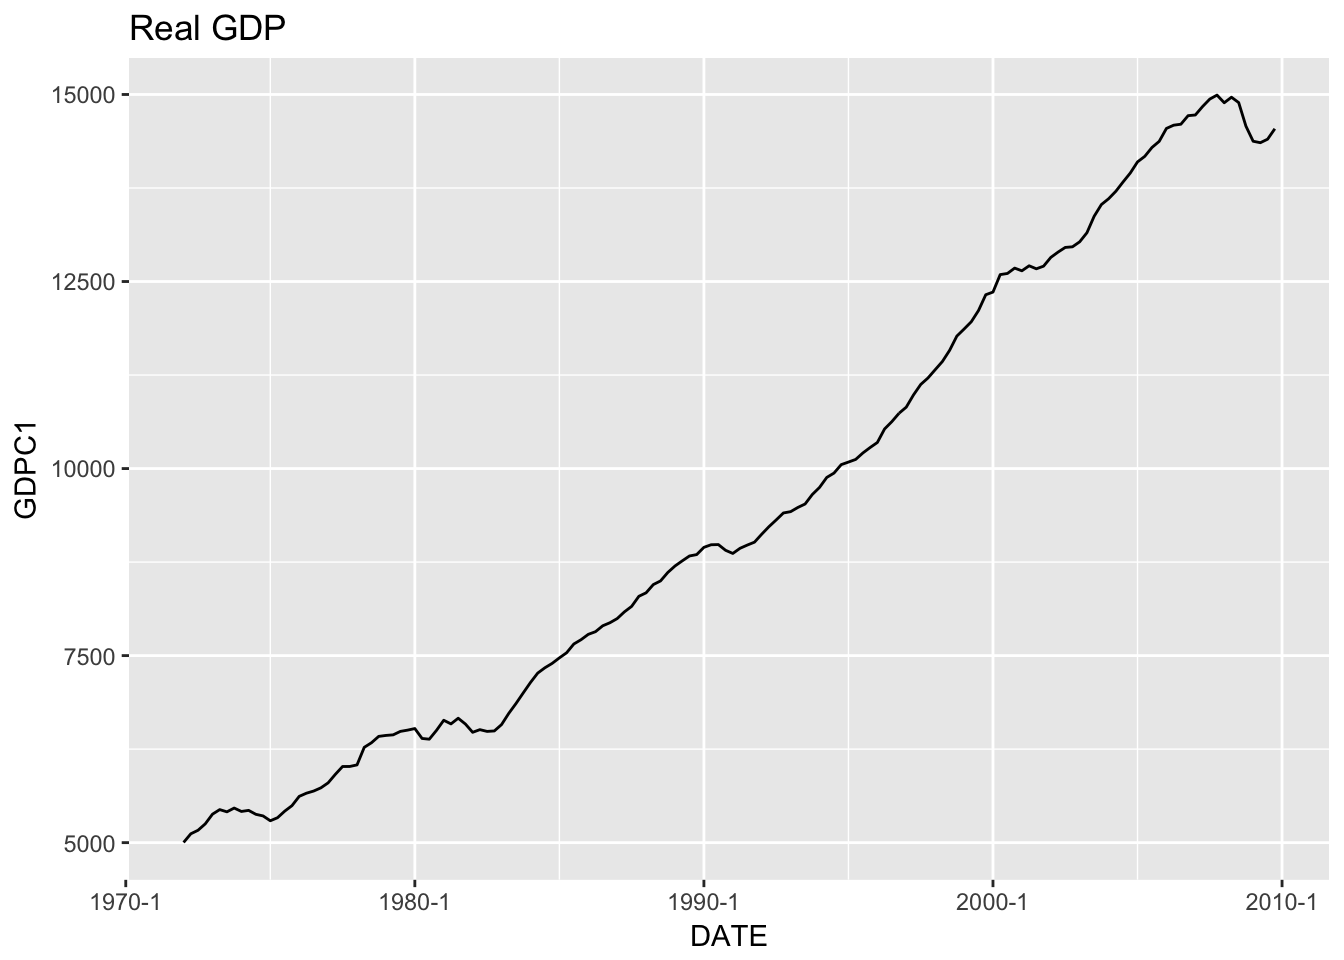
\includegraphics{03-facets-and-bubbles_files/figure-latex/unnamed-chunk-5-1.pdf}

The distribution of this data looks like a good candidate for using the
log scale (high concentration in lower values and lower concentration in
higher values).

\begin{Shaded}
\begin{Highlighting}[]
\NormalTok{seats %>%}
\StringTok{  }\KeywordTok{ggplot}\NormalTok{(}\KeywordTok{aes}\NormalTok{(seats2016, seats2017)) +}
\StringTok{  }\KeywordTok{geom_point}\NormalTok{() +}
\StringTok{  }\KeywordTok{scale_x_log10}\NormalTok{() +}
\StringTok{  }\KeywordTok{scale_y_log10}\NormalTok{() +}\StringTok{ }
\StringTok{  }\KeywordTok{geom_abline}\NormalTok{(}\DataTypeTok{lty =} \DecValTok{2}\NormalTok{) }\CommentTok{# dashed line type (lty)}
\end{Highlighting}
\end{Shaded}

\includegraphics{03-facets-and-bubbles_files/figure-latex/unnamed-chunk-6-1.pdf}

Since we have region identifiers it would be nice to divide our data and
see charts of each region side-by-side. Facets allow us to make multiple
charts based on a variable or set of variables.

\begin{Shaded}
\begin{Highlighting}[]
\NormalTok{seats %>%}
\StringTok{  }\KeywordTok{ggplot}\NormalTok{(}\KeywordTok{aes}\NormalTok{(seats2016, seats2017)) +}
\StringTok{  }\KeywordTok{geom_point}\NormalTok{() +}
\StringTok{  }\KeywordTok{scale_x_log10}\NormalTok{() +}
\StringTok{  }\KeywordTok{scale_y_log10}\NormalTok{() +}\StringTok{ }
\StringTok{  }\KeywordTok{geom_abline}\NormalTok{(}\DataTypeTok{lty =} \DecValTok{2}\NormalTok{) +}
\StringTok{  }\KeywordTok{facet_wrap}\NormalTok{(~}\StringTok{ }\NormalTok{region) +}
\StringTok{  }\KeywordTok{coord_fixed}\NormalTok{()}
\end{Highlighting}
\end{Shaded}

\includegraphics{03-facets-and-bubbles_files/figure-latex/unnamed-chunk-7-1.pdf}

An alternative representation is to present each region using color:

\begin{Shaded}
\begin{Highlighting}[]
\NormalTok{seats %>%}
\StringTok{  }\KeywordTok{ggplot}\NormalTok{(}\KeywordTok{aes}\NormalTok{(seats2016, seats2017, }\DataTypeTok{color =} \NormalTok{region, }\DataTypeTok{label =} \NormalTok{dep_city)) +}
\StringTok{  }\KeywordTok{geom_point}\NormalTok{() +}
\StringTok{  }\KeywordTok{scale_x_log10}\NormalTok{() +}
\StringTok{  }\KeywordTok{scale_y_log10}\NormalTok{() +}\StringTok{ }
\StringTok{  }\KeywordTok{geom_abline}\NormalTok{(}\DataTypeTok{lty =} \DecValTok{2}\NormalTok{) +}
\StringTok{  }\KeywordTok{geom_text}\NormalTok{(}\DataTypeTok{check_overlap =} \OtherTok{TRUE}\NormalTok{, }\DataTypeTok{nudge_y =} \FloatTok{0.1}\NormalTok{)}
\end{Highlighting}
\end{Shaded}

\includegraphics{03-facets-and-bubbles_files/figure-latex/unnamed-chunk-8-1.pdf}

\section{Bubbles}\label{bubbles}

Bubble charts are scatter plots (geom\_point) with points that vary in
size corresponding to the value of a given variable. Let's create a
measure of the size of a city's seats relative to its regional total.

\begin{Shaded}
\begin{Highlighting}[]
\NormalTok{seats <-}\StringTok{ }\NormalTok{seats %>%}
\StringTok{  }\KeywordTok{group_by}\NormalTok{(region) %>%}
\StringTok{  }\KeywordTok{mutate}\NormalTok{(}\DataTypeTok{proportion_of_region =} \NormalTok{seats2017/}\KeywordTok{sum}\NormalTok{(seats2017))}
\NormalTok{seats}
\end{Highlighting}
\end{Shaded}

\begin{verbatim}
## # A tibble: 49 x 18
## # Groups:   region [7]
##          dep_city seats2017Q1 seats2017Q2 seats2017Q3 seats2017Q4
##             <chr>       <dbl>       <dbl>       <dbl>       <dbl>
##  1      Anchorage       25758       15105       13674       17013
##  2     Bellingham       10198         318          NA        6519
##  3         Denver       55803       51654       52585       43290
##  4      Las Vegas       70514       74322       75839       75415
##  5    Los Angeles      548935      647498      715338      647703
##  6        Oakland       84571      104810      116015       90703
##  7        Phoenix      113046      115125      125348      108863
##  8       Portland       90207       71068       65997       81673
##  9     Sacramento       37620       38318       38456       38456
## 10 Salt Lake City       26370       23751       22968       28322
## # ... with 39 more rows, and 13 more variables: seats2017 <dbl>,
## #   seats2016Q1 <dbl>, seats2016Q2 <dbl>, seats2016Q3 <dbl>,
## #   seats2016Q4 <dbl>, seats2016 <dbl>, seatschangeQ1 <dbl>,
## #   seatschangeQ2 <chr>, seatschangeQ3 <chr>, seatschangeQ4 <dbl>,
## #   seatschange <dbl>, region <chr>, proportion_of_region <dbl>
\end{verbatim}

Now we can modify the chart to show the importance of each city in the
context of its region.

\begin{Shaded}
\begin{Highlighting}[]
\NormalTok{seats %>%}
\StringTok{  }\KeywordTok{filter}\NormalTok{(region %in%}\StringTok{ }\KeywordTok{c}\NormalTok{(}\StringTok{"US West"}\NormalTok{, }\StringTok{"US East"}\NormalTok{)) %>%}
\StringTok{  }\KeywordTok{ggplot}\NormalTok{(}\KeywordTok{aes}\NormalTok{(seats2016, seats2017, }\DataTypeTok{color =} \NormalTok{region, }\DataTypeTok{label =} \NormalTok{dep_city)) +}
\StringTok{  }\KeywordTok{geom_abline}\NormalTok{(}\DataTypeTok{lty =} \DecValTok{2}\NormalTok{) +}
\StringTok{  }\KeywordTok{geom_point}\NormalTok{(}\KeywordTok{aes}\NormalTok{(}\DataTypeTok{size =} \NormalTok{proportion_of_region)) +}
\StringTok{  }\KeywordTok{scale_x_log10}\NormalTok{(}\DataTypeTok{labels =} \NormalTok{scales::comma) +}
\StringTok{  }\KeywordTok{scale_y_log10}\NormalTok{(}\DataTypeTok{labels =} \NormalTok{scales::comma) +}\StringTok{ }
\StringTok{  }\KeywordTok{geom_text}\NormalTok{(}\DataTypeTok{check_overlap =} \OtherTok{TRUE}\NormalTok{, }\DataTypeTok{nudge_y =} \FloatTok{0.1}\NormalTok{)}
\end{Highlighting}
\end{Shaded}

\includegraphics{03-facets-and-bubbles_files/figure-latex/unnamed-chunk-10-1.pdf}

\section{Transparency}\label{transparency}

We can also use transparency (or alpha) to make less important points
less visible. We do this by setting the \texttt{alpha} aesthetic. Let's
try adding the alpha setting to the \texttt{geom\_point()} call first.

\begin{Shaded}
\begin{Highlighting}[]
\NormalTok{seats %>%}
\StringTok{  }\KeywordTok{filter}\NormalTok{(region %in%}\StringTok{ }\KeywordTok{c}\NormalTok{(}\StringTok{"US West"}\NormalTok{, }\StringTok{"US East"}\NormalTok{)) %>%}
\StringTok{  }\KeywordTok{ggplot}\NormalTok{(}\KeywordTok{aes}\NormalTok{(seats2016, seats2017, }\DataTypeTok{color =} \NormalTok{region, }\DataTypeTok{label =} \NormalTok{dep_city)) +}
\StringTok{  }\KeywordTok{geom_abline}\NormalTok{(}\DataTypeTok{lty =} \DecValTok{2}\NormalTok{) +}
\StringTok{  }\KeywordTok{geom_point}\NormalTok{(}\KeywordTok{aes}\NormalTok{(}\DataTypeTok{size =} \NormalTok{proportion_of_region, }\DataTypeTok{alpha =} \NormalTok{proportion_of_region)) +}
\StringTok{  }\KeywordTok{scale_x_log10}\NormalTok{(}\DataTypeTok{labels =} \NormalTok{scales::comma) +}
\StringTok{  }\KeywordTok{scale_y_log10}\NormalTok{(}\DataTypeTok{labels =} \NormalTok{scales::comma) +}\StringTok{ }
\StringTok{  }\KeywordTok{geom_text}\NormalTok{(}\DataTypeTok{check_overlap =} \OtherTok{TRUE}\NormalTok{, }\DataTypeTok{nudge_y =} \FloatTok{0.1}\NormalTok{)}
\end{Highlighting}
\end{Shaded}

\includegraphics{03-facets-and-bubbles_files/figure-latex/unnamed-chunk-11-1.pdf}

Let's add the alpha to the ggplot-level aesthetic instead, so that it
also affects the text labels.

\begin{Shaded}
\begin{Highlighting}[]
\NormalTok{seats %>%}
\StringTok{  }\KeywordTok{filter}\NormalTok{(region %in%}\StringTok{ }\KeywordTok{c}\NormalTok{(}\StringTok{"US West"}\NormalTok{, }\StringTok{"US East"}\NormalTok{)) %>%}
\StringTok{  }\KeywordTok{ggplot}\NormalTok{(}\KeywordTok{aes}\NormalTok{(seats2016, seats2017, }\DataTypeTok{color =} \NormalTok{region, }\DataTypeTok{label =} \NormalTok{dep_city, }\DataTypeTok{alpha =} \NormalTok{proportion_of_region)) +}
\StringTok{  }\KeywordTok{geom_abline}\NormalTok{(}\DataTypeTok{lty =} \DecValTok{2}\NormalTok{) +}
\StringTok{  }\KeywordTok{geom_point}\NormalTok{(}\KeywordTok{aes}\NormalTok{(}\DataTypeTok{size =} \NormalTok{proportion_of_region)) +}
\StringTok{  }\KeywordTok{scale_x_log10}\NormalTok{(}\DataTypeTok{labels =} \NormalTok{scales::comma) +}
\StringTok{  }\KeywordTok{scale_y_log10}\NormalTok{(}\DataTypeTok{labels =} \NormalTok{scales::comma) +}\StringTok{ }
\StringTok{  }\KeywordTok{geom_text}\NormalTok{(}\DataTypeTok{nudge_y =} \FloatTok{0.1}\NormalTok{)}
\end{Highlighting}
\end{Shaded}

\includegraphics{03-facets-and-bubbles_files/figure-latex/unnamed-chunk-12-1.pdf}

We can combine all the regions now and use transparency to help us see
how many cities are in the same area on the plot by how dark a region
is.

\begin{Shaded}
\begin{Highlighting}[]
\NormalTok{seats %>%}
\StringTok{  }\KeywordTok{ggplot}\NormalTok{(}\KeywordTok{aes}\NormalTok{(seats2016, seats2017, }\DataTypeTok{label =} \NormalTok{dep_city, }\DataTypeTok{alpha =} \NormalTok{proportion_of_region)) +}
\StringTok{  }\KeywordTok{geom_abline}\NormalTok{(}\DataTypeTok{lty =} \DecValTok{2}\NormalTok{) +}
\StringTok{  }\KeywordTok{geom_point}\NormalTok{(}\KeywordTok{aes}\NormalTok{(}\DataTypeTok{size =} \NormalTok{proportion_of_region)) +}
\StringTok{  }\KeywordTok{scale_x_log10}\NormalTok{(}\DataTypeTok{labels =} \NormalTok{scales::comma) +}
\StringTok{  }\KeywordTok{scale_y_log10}\NormalTok{(}\DataTypeTok{labels =} \NormalTok{scales::comma) +}\StringTok{ }
\StringTok{  }\KeywordTok{geom_text}\NormalTok{(}\KeywordTok{aes}\NormalTok{(}\DataTypeTok{color =} \NormalTok{region), }\DataTypeTok{hjust =} \StringTok{"right"}\NormalTok{, }\DataTypeTok{vjust =} \StringTok{"center"}\NormalTok{)}
\end{Highlighting}
\end{Shaded}

\includegraphics{03-facets-and-bubbles_files/figure-latex/unnamed-chunk-13-1.pdf}

\section{Facets}\label{facets-1}

Let's use facets so we can combine everything we've done so far.

\begin{Shaded}
\begin{Highlighting}[]
\NormalTok{seats %>%}
\StringTok{  }\KeywordTok{ggplot}\NormalTok{(}\KeywordTok{aes}\NormalTok{(seats2016, seats2017, }\DataTypeTok{label =} \NormalTok{dep_city, }\DataTypeTok{alpha =} \NormalTok{proportion_of_region)) +}
\StringTok{  }\KeywordTok{geom_abline}\NormalTok{(}\DataTypeTok{lty =} \DecValTok{2}\NormalTok{) +}
\StringTok{  }\KeywordTok{geom_point}\NormalTok{(}\KeywordTok{aes}\NormalTok{(}\DataTypeTok{size =} \NormalTok{proportion_of_region), }\DataTypeTok{color =} \StringTok{"darkblue"}\NormalTok{) +}
\StringTok{  }\KeywordTok{scale_x_log10}\NormalTok{(}\DataTypeTok{labels =} \NormalTok{scales::comma) +}
\StringTok{  }\KeywordTok{scale_y_log10}\NormalTok{(}\DataTypeTok{labels =} \NormalTok{scales::comma) +}\StringTok{ }
\StringTok{  }\KeywordTok{geom_text}\NormalTok{(}\DataTypeTok{hjust =} \StringTok{"right"}\NormalTok{, }\DataTypeTok{vjust =} \StringTok{"center"}\NormalTok{, }\DataTypeTok{nudge_x =} \NormalTok{-}\FloatTok{0.3}\NormalTok{) +}
\StringTok{  }\KeywordTok{facet_wrap}\NormalTok{(~}\StringTok{ }\NormalTok{region)}
\end{Highlighting}
\end{Shaded}

\includegraphics{03-facets-and-bubbles_files/figure-latex/unnamed-chunk-14-1.pdf}

\section{Assignment}\label{assignment-2}

Create a bubble plot highlighting the change in year-on-year growth
rates for different quarters. Plot \texttt{seatschangeQ3} on the x axis
and \texttt{seatschangeQ4} on the y axis. Use \texttt{seats2017} to
determine the size of each bubble. Facet by region.

\hypertarget{lines}{\chapter{Lines and Curves}\label{lines}}

\section{Data}\label{data-1}

We will use data on the number of active duty personnel in Hawaii. The
first dataset is an Excel file pulled from the State of Hawaii
Department of Business, Economic Development, and Tourism (DBEDT)
\href{http://dbedt.hawaii.gov/economic/databook/2015-individual/}{2015
State of Hawaii Data Book}. See the line listed as, ``10.03 - Active
Duty Personnel, by Service: 1953 to 2015.'' The data is originally from
the \href{www.dmdc.osd.mil/appj/dwp/stats_reports.jsp}{US Defense
Manpower Data Center}

\begin{Shaded}
\begin{Highlighting}[]
\KeywordTok{library}\NormalTok{(tidyverse)}
\KeywordTok{library}\NormalTok{(readxl)}
\end{Highlighting}
\end{Shaded}

\begin{Shaded}
\begin{Highlighting}[]
\NormalTok{mil_personnel <-}\StringTok{ }\KeywordTok{read_excel}\NormalTok{(}\StringTok{"data/100315.xls"}\NormalTok{, }\DataTypeTok{range =} \StringTok{"A5:L38"}\NormalTok{, }\DataTypeTok{col_types =} \StringTok{"numeric"}\NormalTok{)}
\NormalTok{mil_personnel <-}\StringTok{ }\KeywordTok{bind_rows}\NormalTok{(}
  \NormalTok{mil_personnel %>%}\StringTok{ }\KeywordTok{select}\NormalTok{(}\DecValTok{1}\NormalTok{:}\DecValTok{6}\NormalTok{) %>%}\StringTok{ }\NormalTok{magrittr::}\KeywordTok{set_colnames}\NormalTok{(}\KeywordTok{c}\NormalTok{(}\StringTok{"Year"}\NormalTok{, }\StringTok{"Total"}\NormalTok{, }\StringTok{"Army"}\NormalTok{, }\StringTok{"Navy"}\NormalTok{, }\StringTok{"Marine Corps"}\NormalTok{, }\StringTok{"Air Force"}\NormalTok{)),}
  \NormalTok{mil_personnel %>%}\StringTok{ }\KeywordTok{select}\NormalTok{(}\DecValTok{7}\NormalTok{:}\DecValTok{12}\NormalTok{) %>%}\StringTok{ }\NormalTok{magrittr::}\KeywordTok{set_colnames}\NormalTok{(}\KeywordTok{c}\NormalTok{(}\StringTok{"Year"}\NormalTok{, }\StringTok{"Total"}\NormalTok{, }\StringTok{"Army"}\NormalTok{, }\StringTok{"Navy"}\NormalTok{, }\StringTok{"Marine Corps"}\NormalTok{, }\StringTok{"Air Force"}\NormalTok{))}
\NormalTok{)}
\NormalTok{mil_personnel}
\end{Highlighting}
\end{Shaded}

\begin{verbatim}
## # A tibble: 66 x 6
##     Year Total  Army  Navy `Marine Corps` `Air Force`
##    <dbl> <dbl> <dbl> <dbl>          <dbl>       <dbl>
##  1    NA    NA    NA    NA             NA          NA
##  2  1953 24785  5872  7657           6040        5216
##  3  1954 23654  7957  6443           4155        5099
##  4  1955 40258 19821  5211           9677        5549
##  5  1956 37470 16531  5237           9490        6212
##  6  1957 40683 17511  5466           9608        8098
##  7  1958 35076 14672  4908           8670        6826
##  8  1959 36310 15438  5309           8470        7093
##  9  1960 35412 15492  5687           7756        6477
## 10  1961 39474 16945  5774           9679        7076
## # ... with 56 more rows
\end{verbatim}

Notice that the \texttt{Year} 2015 was turned into \texttt{NA}. This
happened because the value in the corresponding cell was `2/ 2015'.
Let's remove the final row of \texttt{NA}s and replace the remaining
\texttt{NA} with 2015.

\begin{Shaded}
\begin{Highlighting}[]
\NormalTok{mil_personnel <-}\StringTok{ }\NormalTok{mil_personnel %>%}\StringTok{ }\KeywordTok{filter}\NormalTok{(!}\KeywordTok{is.na}\NormalTok{(Total))}
\NormalTok{mil_personnel[}\KeywordTok{is.na}\NormalTok{(mil_personnel$Year),]$Year <-}\StringTok{ }\DecValTok{2015}
\NormalTok{mil_personnel}
\end{Highlighting}
\end{Shaded}

\begin{verbatim}
## # A tibble: 63 x 6
##     Year Total  Army  Navy `Marine Corps` `Air Force`
##    <dbl> <dbl> <dbl> <dbl>          <dbl>       <dbl>
##  1  1953 24785  5872  7657           6040        5216
##  2  1954 23654  7957  6443           4155        5099
##  3  1955 40258 19821  5211           9677        5549
##  4  1956 37470 16531  5237           9490        6212
##  5  1957 40683 17511  5466           9608        8098
##  6  1958 35076 14672  4908           8670        6826
##  7  1959 36310 15438  5309           8470        7093
##  8  1960 35412 15492  5687           7756        6477
##  9  1961 39474 16945  5774           9679        7076
## 10  1962 41657 17645  6664           9903        7445
## # ... with 53 more rows
\end{verbatim}

\section{geom\_smooth}\label{geom_smooth}

\texttt{geom\_smooth} allows you to have smooth lines appear in your
chart. With no argument, it will choose \texttt{loess} for series
shorter than 1,000 observations. It shows a shaded confidence interval.

\begin{Shaded}
\begin{Highlighting}[]
\NormalTok{mil_personnel %>%}
\StringTok{  }\KeywordTok{ggplot}\NormalTok{(}\KeywordTok{aes}\NormalTok{(Year, Total)) +}
\StringTok{  }\KeywordTok{geom_point}\NormalTok{() +}
\StringTok{  }\KeywordTok{geom_smooth}\NormalTok{()}
\end{Highlighting}
\end{Shaded}

\includegraphics{04-lines_files/figure-latex/unnamed-chunk-6-1.pdf}

Here's what it looks like if we fit a linear model instead:

\begin{Shaded}
\begin{Highlighting}[]
\NormalTok{mil_personnel %>%}
\StringTok{  }\KeywordTok{ggplot}\NormalTok{(}\KeywordTok{aes}\NormalTok{(Year, Total)) +}
\StringTok{  }\KeywordTok{geom_point}\NormalTok{() +}
\StringTok{  }\KeywordTok{geom_smooth}\NormalTok{(}\DataTypeTok{method =} \StringTok{"lm"}\NormalTok{)}
\end{Highlighting}
\end{Shaded}

\includegraphics{04-lines_files/figure-latex/unnamed-chunk-7-1.pdf}

We can also just have a line chart that connects the points:

\begin{Shaded}
\begin{Highlighting}[]
\NormalTok{mil_personnel %>%}
\StringTok{  }\KeywordTok{ggplot}\NormalTok{(}\KeywordTok{aes}\NormalTok{(Year, Total)) +}
\StringTok{  }\KeywordTok{geom_point}\NormalTok{() +}
\StringTok{  }\KeywordTok{geom_line}\NormalTok{()}
\end{Highlighting}
\end{Shaded}

\includegraphics{04-lines_files/figure-latex/unnamed-chunk-8-1.pdf}

\section{geom\_abline}\label{geom_abline}

\texttt{geom\_abline} allows you to display lines with a specific
intercept and slope. If no intercept or slope is provided, a 45-degree
line will be shown.

\begin{Shaded}
\begin{Highlighting}[]
\NormalTok{x =}\StringTok{ }\KeywordTok{rnorm}\NormalTok{(}\DecValTok{100}\NormalTok{)}
\NormalTok{y =}\StringTok{ }\FloatTok{2.5} \NormalTok{+}\StringTok{ }\FloatTok{1.2} \NormalTok{*}\StringTok{ }\NormalTok{x +}\StringTok{ }\KeywordTok{rnorm}\NormalTok{(}\DecValTok{100}\NormalTok{)}
\NormalTok{test_data <-}\StringTok{ }\KeywordTok{data_frame}\NormalTok{(x, y)}

\NormalTok{test_data %>%}\StringTok{ }
\StringTok{  }\KeywordTok{ggplot}\NormalTok{(}\KeywordTok{aes}\NormalTok{(x, y)) +}
\StringTok{  }\KeywordTok{geom_point}\NormalTok{() +}
\StringTok{  }\KeywordTok{xlim}\NormalTok{(-}\DecValTok{2}\NormalTok{, }\DecValTok{6}\NormalTok{) +}\StringTok{ }\KeywordTok{ylim}\NormalTok{(-}\DecValTok{2}\NormalTok{, }\DecValTok{6}\NormalTok{) +}
\StringTok{  }\KeywordTok{coord_fixed}\NormalTok{() +}
\StringTok{  }\KeywordTok{geom_abline}\NormalTok{() }
\end{Highlighting}
\end{Shaded}

\includegraphics{04-lines_files/figure-latex/unnamed-chunk-9-1.pdf}

\begin{Shaded}
\begin{Highlighting}[]
\NormalTok{test_data %>%}\StringTok{ }
\StringTok{  }\KeywordTok{ggplot}\NormalTok{(}\KeywordTok{aes}\NormalTok{(x, y)) +}
\StringTok{  }\KeywordTok{geom_point}\NormalTok{() +}
\StringTok{  }\KeywordTok{xlim}\NormalTok{(-}\DecValTok{2}\NormalTok{, }\DecValTok{6}\NormalTok{) +}\StringTok{ }\KeywordTok{ylim}\NormalTok{(-}\DecValTok{2}\NormalTok{, }\DecValTok{6}\NormalTok{) +}
\StringTok{  }\KeywordTok{coord_fixed}\NormalTok{() +}
\StringTok{  }\KeywordTok{geom_abline}\NormalTok{() +}
\StringTok{  }\KeywordTok{geom_abline}\NormalTok{(}\DataTypeTok{intercept =} \FloatTok{2.5}\NormalTok{, }\DataTypeTok{slope =} \FloatTok{1.2}\NormalTok{, }\DataTypeTok{color =} \StringTok{"red"}\NormalTok{) }
\end{Highlighting}
\end{Shaded}

\includegraphics{04-lines_files/figure-latex/unnamed-chunk-10-1.pdf}

\section{geom\_vline}\label{geom_vline}

\texttt{geom\_vline} allows you to draw vertical lines by specifying an
x intercept.

\begin{Shaded}
\begin{Highlighting}[]
\NormalTok{test_data %>%}\StringTok{ }
\StringTok{  }\KeywordTok{ggplot}\NormalTok{(}\KeywordTok{aes}\NormalTok{(x, y)) +}
\StringTok{  }\KeywordTok{geom_point}\NormalTok{() +}
\StringTok{  }\KeywordTok{xlim}\NormalTok{(-}\DecValTok{2}\NormalTok{, }\DecValTok{6}\NormalTok{) +}\StringTok{ }\KeywordTok{ylim}\NormalTok{(-}\DecValTok{2}\NormalTok{, }\DecValTok{6}\NormalTok{) +}
\StringTok{  }\KeywordTok{coord_fixed}\NormalTok{() +}
\StringTok{  }\KeywordTok{geom_abline}\NormalTok{() +}
\StringTok{  }\KeywordTok{geom_abline}\NormalTok{(}\DataTypeTok{intercept =} \FloatTok{2.5}\NormalTok{, }\DataTypeTok{slope =} \FloatTok{1.2}\NormalTok{, }\DataTypeTok{color =} \StringTok{"red"}\NormalTok{) +}
\StringTok{  }\KeywordTok{geom_vline}\NormalTok{(}\DataTypeTok{xintercept =} \DecValTok{2}\NormalTok{, }\DataTypeTok{color =} \StringTok{"blue"}\NormalTok{)}
\end{Highlighting}
\end{Shaded}

\includegraphics{04-lines_files/figure-latex/unnamed-chunk-11-1.pdf}

\section{hline}\label{hline}

\texttt{geom\_vline} allows you to draw vertical lines by specifying an
x intercept.

\begin{Shaded}
\begin{Highlighting}[]
\NormalTok{test_data %>%}\StringTok{ }
\StringTok{  }\KeywordTok{ggplot}\NormalTok{(}\KeywordTok{aes}\NormalTok{(x, y)) +}
\StringTok{  }\KeywordTok{geom_point}\NormalTok{() +}
\StringTok{  }\KeywordTok{xlim}\NormalTok{(-}\DecValTok{2}\NormalTok{, }\DecValTok{6}\NormalTok{) +}\StringTok{ }\KeywordTok{ylim}\NormalTok{(-}\DecValTok{2}\NormalTok{, }\DecValTok{6}\NormalTok{) +}
\StringTok{  }\KeywordTok{coord_fixed}\NormalTok{() +}
\StringTok{  }\KeywordTok{geom_abline}\NormalTok{() +}
\StringTok{  }\KeywordTok{geom_abline}\NormalTok{(}\DataTypeTok{intercept =} \FloatTok{2.5}\NormalTok{, }\DataTypeTok{slope =} \FloatTok{1.2}\NormalTok{, }\DataTypeTok{color =} \StringTok{"red"}\NormalTok{) +}
\StringTok{  }\KeywordTok{geom_vline}\NormalTok{(}\DataTypeTok{xintercept =} \DecValTok{2}\NormalTok{, }\DataTypeTok{color =} \StringTok{"blue"}\NormalTok{) +}
\StringTok{  }\KeywordTok{geom_hline}\NormalTok{(}\DataTypeTok{yintercept =} \DecValTok{1}\NormalTok{, }\DataTypeTok{color =} \StringTok{"#4FCC53"}\NormalTok{, }\DataTypeTok{lty =} \DecValTok{2}\NormalTok{)}
\end{Highlighting}
\end{Shaded}

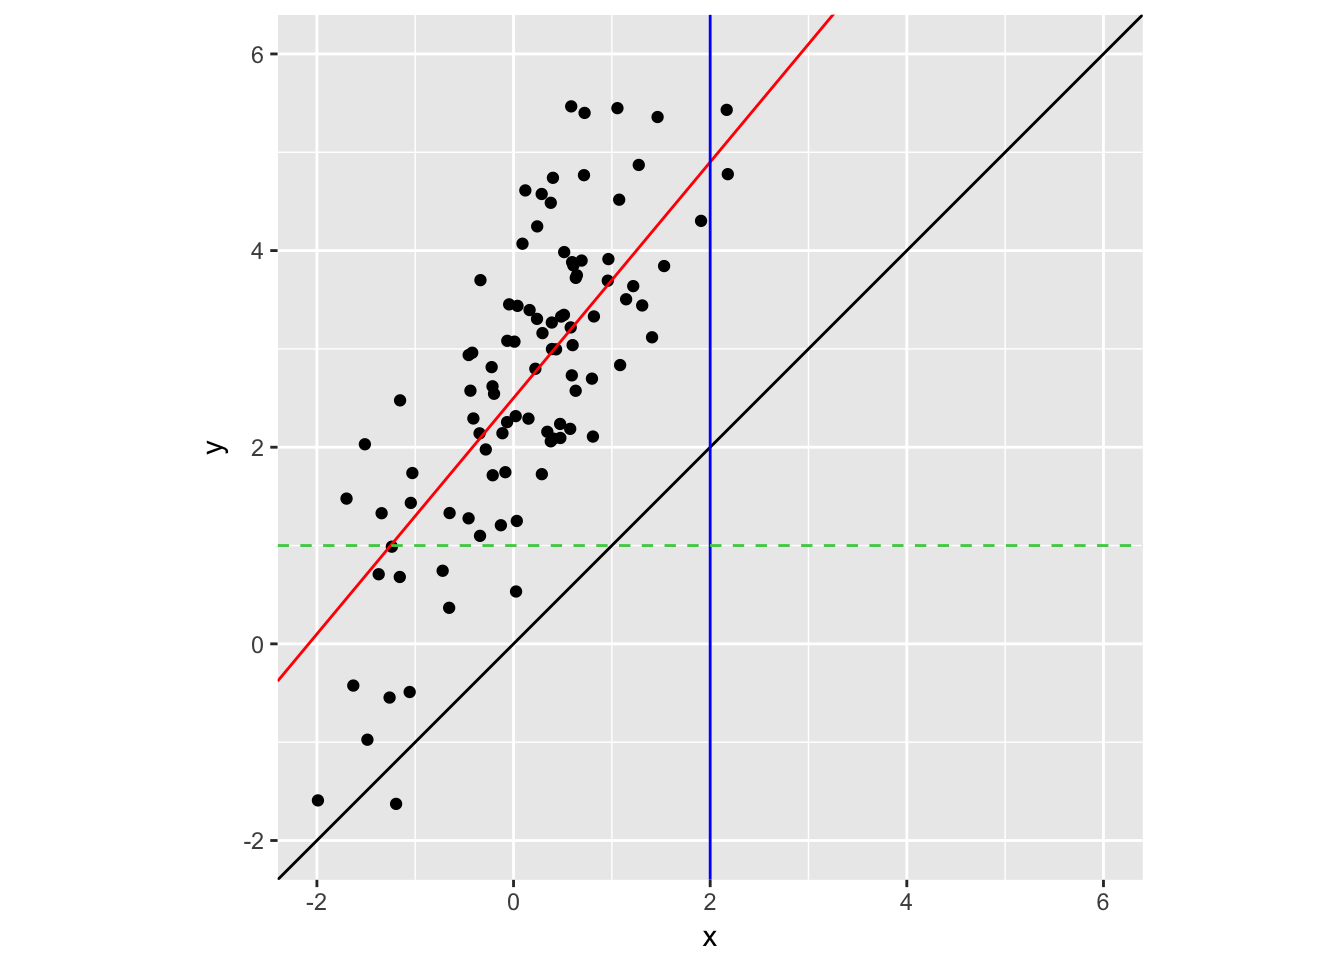
\includegraphics{04-lines_files/figure-latex/lines-vline-1.pdf}

\section{Assignment}\label{assignment-3}

Create a visualization of the military data by branch (i.e.,
\texttt{Army}, \texttt{Navy}, etc.) using \texttt{facet\_wrap()}. Plot
both the points and a smooth line.

The data we have been working with is not yet
\href{http://tidyr.tidyverse.org/}{tidy}. Each row contains multiple
observations (observations for Army, Navy, etc.). To make this tidy we
should have one column with the personnel counts and one column that
indicates the branch.

\begin{Shaded}
\begin{Highlighting}[]
\NormalTok{tidy_mil <-}\StringTok{ }\NormalTok{mil_personnel %>%}
\StringTok{  }\KeywordTok{gather}\NormalTok{(branch, personnel, -Year)}
\NormalTok{tidy_mil}
\end{Highlighting}
\end{Shaded}

\begin{verbatim}
## # A tibble: 315 x 3
##     Year branch personnel
##    <dbl>  <chr>     <dbl>
##  1  1953  Total     24785
##  2  1954  Total     23654
##  3  1955  Total     40258
##  4  1956  Total     37470
##  5  1957  Total     40683
##  6  1958  Total     35076
##  7  1959  Total     36310
##  8  1960  Total     35412
##  9  1961  Total     39474
## 10  1962  Total     41657
## # ... with 305 more rows
\end{verbatim}

\hypertarget{ggplot-exts}{\chapter{Scatter Plot Matrices and
Extensions}\label{ggplot-exts}}

\section{Data}\label{data-2}

For this section, we'll look at data from the American Community Survey
(ACS) on immigration. To download the data,

\begin{enumerate}
\def\labelenumi{\arabic{enumi}.}
\tightlist
\item
  Go to the \href{https://factfinder.census.gov/}{American FactFinder
  website}.
\item
  Click on the ``Download Center'' section, then click the ``DOWNLOAD
  CENTER'' button.
\item
  Click the ``NEXT'' button, since we know the table we want to
  download.
\item
  Select ``American Community Survey'' from the Program dropdown.
\item
  Select ``2015 ACS 5-year estimates'', click the ``ADD TO YOUR
  SELECTIONS'' button, then click ``NEXT''
\item
  Select ``County - 050'' from the geographic type dropdown, then select
  ``All Counties within United States'', click the ``ADD TO YOUR
  SELECTIONS'' button, then click ``NEXT''
\item
  Type \texttt{income\ mobility} in the ``topic or table name''" search
  box, then select the option that reads:
\end{enumerate}

``B07011: MEDIAN INCOME IN THE PAST 12 MONTHS (IN 2015
INFLATION-ADJUSTED DOLLARS) BY GEOGRAPHICAL MOBILITY IN THE PAST YEAR
FOR CURRENT RESIDENCE IN THE UNITED STATES''

Click ``GO'', then check the checkbox beside the table we found. Now
click on the ``Download'' button, and uncheck the option that says,
``Include descriptive data element names.'' Click ``Ok'' to create your
zip file. Once the file has been created, click ``DOWNLOAD'' to download
the zip file.

The following will assume you moved the following files within the zip
to your \texttt{data} folder:

\begin{itemize}
\tightlist
\item
  ACS\_15\_5YR\_B07011\_with\_ann.csv
\item
  ACS\_15\_5YR\_B07011\_metadata.csv
\end{itemize}

The file \texttt{ACS\_15\_5YR\_B07011.txt} tells us how to interpret
codes within our data. It is possible for median values to be followed
by a \texttt{+} or \texttt{-} if they are in the upper or lower
open-ended interval. In our dataset we don't have any medians in the
upper open-ended interval, but we do have entries in the lower
open-ended interval.

\begin{Shaded}
\begin{Highlighting}[]
\KeywordTok{library}\NormalTok{(tidyverse)}
\end{Highlighting}
\end{Shaded}

\begin{Shaded}
\begin{Highlighting}[]
\NormalTok{acs <-}\StringTok{ }\KeywordTok{read_csv}\NormalTok{(}\StringTok{"data/ACS_15_5YR_B07011_with_ann.csv"}\NormalTok{, }\DataTypeTok{col_types =} \KeywordTok{strrep}\NormalTok{(}\StringTok{"c"}\NormalTok{, }\DecValTok{15}\NormalTok{), }\DataTypeTok{na =} \KeywordTok{c}\NormalTok{(}\StringTok{"-"}\NormalTok{, }\StringTok{"(X)"}\NormalTok{))}
\NormalTok{meta <-}\StringTok{ }\KeywordTok{read_csv}\NormalTok{(}\StringTok{"data/ACS_15_5YR_B07011_metadata.csv"}\NormalTok{)}
\NormalTok{meta}
\end{Highlighting}
\end{Shaded}

\begin{verbatim}
## # A tibble: 14 x 2
##               GEO.id
##                <chr>
##  1           GEO.id2
##  2 GEO.display-label
##  3         HD01_VD02
##  4         HD02_VD02
##  5         HD01_VD03
##  6         HD02_VD03
##  7         HD01_VD04
##  8         HD02_VD04
##  9         HD01_VD05
## 10         HD02_VD05
## 11         HD01_VD06
## 12         HD02_VD06
## 13         HD01_VD07
## 14         HD02_VD07
## # ... with 1 more variables: Id <chr>
\end{verbatim}

Let's keep only the variables we care about, using more informative
variable names.

\begin{Shaded}
\begin{Highlighting}[]
\NormalTok{acs_mobility <-}\StringTok{ }\NormalTok{acs %>%}
\StringTok{  }\KeywordTok{transmute}\NormalTok{(}
    \DataTypeTok{geo =} \StringTok{`}\DataTypeTok{GEO.display-label}\StringTok{`}\NormalTok{,}
    \DataTypeTok{same_house =} \NormalTok{HD01_VD03,}
    \DataTypeTok{same_county =} \NormalTok{HD01_VD04,}
    \DataTypeTok{same_state =} \NormalTok{HD01_VD05,}
    \DataTypeTok{same_country =} \NormalTok{HD01_VD06,}
    \DataTypeTok{different_country =} \NormalTok{HD01_VD07}
  \NormalTok{)}
\NormalTok{acs_mobility}
\end{Highlighting}
\end{Shaded}

\begin{verbatim}
## # A tibble: 1,949 x 6
##                         geo same_house same_county same_state same_country
##                       <chr>      <chr>       <chr>      <chr>        <chr>
##  1  Autauga County, Alabama      27553       18655      27643        35870
##  2  Barbour County, Alabama      17263       17363       8165        12667
##  3     Bibb County, Alabama      21489       16112       8804         <NA>
##  4   Butler County, Alabama      19499       11734      20769        23887
##  5 Chambers County, Alabama      20708       14522      21218        18516
##  6  Chilton County, Alabama      23668       20646      15739        33464
##  7     Clay County, Alabama      19201       18836      20596        11350
##  8 Cleburne County, Alabama      21888       11583      20380        16475
##  9   Coffee County, Alabama      24325       18957      11906        31702
## 10  Colbert County, Alabama      22419       18389      17330        20093
## # ... with 1,939 more rows, and 1 more variables: different_country <chr>
\end{verbatim}

Now we can add an indicator for whether the median value is in the
lowest available interval. This would mean that the median value
presented has been bottom-coded.

\begin{Shaded}
\begin{Highlighting}[]
\NormalTok{acs_mobility <-}\StringTok{ }\NormalTok{acs_mobility %>%}
\StringTok{  }\KeywordTok{mutate}\NormalTok{(}
    \DataTypeTok{same_country_bc =} \KeywordTok{grepl}\NormalTok{(}\StringTok{"[0-9]*-"}\NormalTok{, same_country),}
    \DataTypeTok{different_country_bc =} \KeywordTok{grepl}\NormalTok{(}\StringTok{"[0-9]*-"}\NormalTok{, different_country)}
  \NormalTok{)}
\NormalTok{acs_mobility}
\end{Highlighting}
\end{Shaded}

\begin{verbatim}
## # A tibble: 1,949 x 8
##                         geo same_house same_county same_state same_country
##                       <chr>      <chr>       <chr>      <chr>        <chr>
##  1  Autauga County, Alabama      27553       18655      27643        35870
##  2  Barbour County, Alabama      17263       17363       8165        12667
##  3     Bibb County, Alabama      21489       16112       8804         <NA>
##  4   Butler County, Alabama      19499       11734      20769        23887
##  5 Chambers County, Alabama      20708       14522      21218        18516
##  6  Chilton County, Alabama      23668       20646      15739        33464
##  7     Clay County, Alabama      19201       18836      20596        11350
##  8 Cleburne County, Alabama      21888       11583      20380        16475
##  9   Coffee County, Alabama      24325       18957      11906        31702
## 10  Colbert County, Alabama      22419       18389      17330        20093
## # ... with 1,939 more rows, and 3 more variables: different_country <chr>,
## #   same_country_bc <lgl>, different_country_bc <lgl>
\end{verbatim}

Let's see how many counties have observations that are bottom coded:

\begin{Shaded}
\begin{Highlighting}[]
\NormalTok{acs_mobility %>%}
\StringTok{  }\KeywordTok{summarize}\NormalTok{(}\DataTypeTok{same_country_bc =} \KeywordTok{sum}\NormalTok{(same_country_bc), }\DataTypeTok{different_country_bc =} \KeywordTok{sum}\NormalTok{(different_country_bc), }\DataTypeTok{counties =} \KeywordTok{n}\NormalTok{())}
\end{Highlighting}
\end{Shaded}

\begin{verbatim}
## # A tibble: 1 x 3
##   same_country_bc different_country_bc counties
##             <int>                <int>    <int>
## 1              15                   64     1949
\end{verbatim}

Let's see what the typical bottom-coded values are:

\begin{Shaded}
\begin{Highlighting}[]
\NormalTok{acs_mobility %>%}
\StringTok{  }\KeywordTok{filter}\NormalTok{(same_country_bc) %>%}
\StringTok{  }\KeywordTok{select}\NormalTok{(same_country) %>%}
\StringTok{  }\KeywordTok{table}\NormalTok{()}
\end{Highlighting}
\end{Shaded}

\begin{verbatim}
## .
## 2,500- 
##     15
\end{verbatim}

\begin{Shaded}
\begin{Highlighting}[]
\NormalTok{acs_mobility %>%}
\StringTok{  }\KeywordTok{filter}\NormalTok{(different_country_bc) %>%}
\StringTok{  }\KeywordTok{select}\NormalTok{(different_country) %>%}
\StringTok{  }\KeywordTok{table}\NormalTok{()}
\end{Highlighting}
\end{Shaded}

\begin{verbatim}
## .
## 2,500- 
##     64
\end{verbatim}

In both cases the bottom-coded interval is the range from zero to 2,500.
Since this is a small number of counties given the entire range, let's
simply set the bottom-coded values to equal the upper-bound of their
interval (i.e., 2,500).

\begin{Shaded}
\begin{Highlighting}[]
\NormalTok{acs_mobility <-}\StringTok{ }\NormalTok{acs_mobility %>%}
\StringTok{  }\KeywordTok{transmute}\NormalTok{(}
    \DataTypeTok{geo =} \NormalTok{geo,}
    \DataTypeTok{same_house =} \KeywordTok{if_else}\NormalTok{(}\KeywordTok{grepl}\NormalTok{(}\StringTok{"[0-9]*-"}\NormalTok{, same_house), 2500L, }\KeywordTok{as.integer}\NormalTok{(same_house)),}
    \DataTypeTok{same_county =} \KeywordTok{if_else}\NormalTok{(}\KeywordTok{grepl}\NormalTok{(}\StringTok{"[0-9]*-"}\NormalTok{, same_county), 2500L, }\KeywordTok{as.integer}\NormalTok{(same_county)),}
    \DataTypeTok{same_state =} \KeywordTok{if_else}\NormalTok{(}\KeywordTok{grepl}\NormalTok{(}\StringTok{"[0-9]*-"}\NormalTok{, same_state), 2500L, }\KeywordTok{as.integer}\NormalTok{(same_state)),}
    \DataTypeTok{same_country =} \KeywordTok{if_else}\NormalTok{(same_country_bc, 2500L, }\KeywordTok{as.integer}\NormalTok{(same_country)),}
    \DataTypeTok{different_country =} \KeywordTok{if_else}\NormalTok{(different_country_bc, 2500L, }\KeywordTok{as.integer}\NormalTok{(different_country))}
  \NormalTok{)}
\NormalTok{acs_mobility}
\end{Highlighting}
\end{Shaded}

\begin{verbatim}
## # A tibble: 1,949 x 6
##                         geo same_house same_county same_state same_country
##                       <chr>      <int>       <int>      <int>        <int>
##  1  Autauga County, Alabama      27553       18655      27643        35870
##  2  Barbour County, Alabama      17263       17363       8165        12667
##  3     Bibb County, Alabama      21489       16112       8804           NA
##  4   Butler County, Alabama      19499       11734      20769        23887
##  5 Chambers County, Alabama      20708       14522      21218        18516
##  6  Chilton County, Alabama      23668       20646      15739        33464
##  7     Clay County, Alabama      19201       18836      20596        11350
##  8 Cleburne County, Alabama      21888       11583      20380        16475
##  9   Coffee County, Alabama      24325       18957      11906        31702
## 10  Colbert County, Alabama      22419       18389      17330        20093
## # ... with 1,939 more rows, and 1 more variables: different_country <int>
\end{verbatim}

Let's rearrange the data into \texttt{tidy} format (one observation per
row).

\begin{Shaded}
\begin{Highlighting}[]
\NormalTok{tidy_acs <-}\StringTok{ }\NormalTok{acs_mobility %>%}
\StringTok{  }\KeywordTok{gather}\NormalTok{(location_last_year, median_income, -geo, }\DataTypeTok{factor_key =} \OtherTok{TRUE}\NormalTok{)}
\NormalTok{tidy_acs}
\end{Highlighting}
\end{Shaded}

\begin{verbatim}
## # A tibble: 9,745 x 3
##                         geo location_last_year median_income
##                       <chr>             <fctr>         <int>
##  1  Autauga County, Alabama         same_house         27553
##  2  Barbour County, Alabama         same_house         17263
##  3     Bibb County, Alabama         same_house         21489
##  4   Butler County, Alabama         same_house         19499
##  5 Chambers County, Alabama         same_house         20708
##  6  Chilton County, Alabama         same_house         23668
##  7     Clay County, Alabama         same_house         19201
##  8 Cleburne County, Alabama         same_house         21888
##  9   Coffee County, Alabama         same_house         24325
## 10  Colbert County, Alabama         same_house         22419
## # ... with 9,735 more rows
\end{verbatim}

\section{ggplot2 extensions}\label{ggplot2-extensions}

There are many extensions the community have made that build on ggplot2.
The following link provides a gallery of many of these extensions:

\href{http://www.ggplot2-exts.org/gallery}{ggplot2 extensions}

Some others that are usefull are \texttt{ggjoy} and \texttt{GGally}.

\section{ggjoy}\label{ggjoy}

Make sure \texttt{ggjoy} is installed.

\begin{verbatim}
install.packages("ggjoy")
\end{verbatim}

\texttt{ggjoy} gives us the ability to stack kernel density plots.

\begin{Shaded}
\begin{Highlighting}[]
\KeywordTok{ggplot}\NormalTok{(tidy_acs, }\KeywordTok{aes}\NormalTok{(}\DataTypeTok{x =} \NormalTok{median_income, }\DataTypeTok{y =} \NormalTok{location_last_year, }\KeywordTok{group}\NormalTok{(location_last_year))) +}
\StringTok{  }\NormalTok{ggjoy::}\KeywordTok{geom_joy}\NormalTok{() +}
\StringTok{  }\NormalTok{ggjoy::}\KeywordTok{theme_joy}\NormalTok{()}
\end{Highlighting}
\end{Shaded}

\includegraphics{05-ggplot-exts_files/figure-latex/unnamed-chunk-11-1.pdf}

This plot shows us that, on average, the distance moved in the past year
is inversely related to median income.

\section{scatterplot matrix
(GGally::ggscatmat)}\label{scatterplot-matrix-ggallyggscatmat}

Make sure you have \texttt{GGally} installed.

\begin{verbatim}
install.packages("GGally")
\end{verbatim}

One particular library, \href{http://ggobi.github.io/ggally/}{GGally},
has a great set of visualizations to extend those that come prebuilt
with \texttt{ggplot}. One common visualization tool that is missing from
ggplot is the scatterplot matrix. While base R provides \texttt{splom()}
in the \texttt{lattice} library, \texttt{GGally::ggpairs} and
\texttt{GGally::ggscatmat} pr ovide an easy tool to create a scatterplot
matrix with ggplot2.

\begin{Shaded}
\begin{Highlighting}[]
\NormalTok{acs_mobility %>%}
\StringTok{  }\KeywordTok{as.data.frame}\NormalTok{() %>%}
\StringTok{  }\NormalTok{GGally::}\KeywordTok{ggscatmat}\NormalTok{(}\DataTypeTok{columns =} \DecValTok{2}\NormalTok{:}\KeywordTok{ncol}\NormalTok{(.), }\DataTypeTok{alpha =} \FloatTok{0.1}\NormalTok{)}
\end{Highlighting}
\end{Shaded}

\includegraphics{05-ggplot-exts_files/figure-latex/unnamed-chunk-12-1.pdf}

\section{Assignment}\label{assignment-4}

Go to \href{https://factfinder.census.gov/}{American FactFinder}. Follow
the steps above up until the point where we typed out ``income
mobility''. This time pick another keyword to search for and select a
different table to analyze (make sure this will give you more than two
columns of data you would like to compare). Use \texttt{ggscatmat()} to
visualize the variables that interest you. Keep the filenames as they
are provided by the Census, so I can run your R Markdown file.

\hypertarget{boxplots-and-violins}{\chapter{Boxplots and Violin
Plots}\label{boxplots-and-violins}}

Boxplots and violin plots are two important tools for visualizing the
distribution of data within a dataset. The boxplot highlights the
median, key percentiles, and outliers within a dataset. The violin plot
takes a kernel density plot, rotates it 90 degrees, then mirrors it
about the axis to create a shape that sometimes resembles a violin.

\section{Data}\label{data-3}

The Social Security Administration releases data on earnings and
employment each year. We'll take a look at the data for 2014:

\url{https://www.ssa.gov/policy/docs/statcomps/eedata_sc/2014/index.html}

We're going to download Table 1: ``Number of persons with Social
Security (OASDI) taxable earnings, amount taxable, and contributions, by
state or other area, sex, and type of earnings, 2014''

Save that file as `ssa\_earnings.xlsx' in the \texttt{data} folder

\begin{Shaded}
\begin{Highlighting}[]
\KeywordTok{library}\NormalTok{(tidyverse)}
\KeywordTok{library}\NormalTok{(readxl)}
\end{Highlighting}
\end{Shaded}

\begin{Shaded}
\begin{Highlighting}[]
\NormalTok{ssa <-}\StringTok{ }\KeywordTok{read_xlsx}\NormalTok{(}\StringTok{"data/ssa_earnings.xlsx"}\NormalTok{, }\DataTypeTok{range =} \StringTok{"A7:J159"}\NormalTok{, }
                 \DataTypeTok{col_names =} \KeywordTok{c}\NormalTok{(}\StringTok{"state"}\NormalTok{, }\StringTok{"gender"}\NormalTok{, }\StringTok{"other"}\NormalTok{, }\StringTok{"other2"}\NormalTok{, }\StringTok{"number.total"}\NormalTok{, }\StringTok{"number.wage"}\NormalTok{, }\StringTok{"number.self"}\NormalTok{, }
                               \StringTok{"earnings.total"}\NormalTok{, }\StringTok{"earnings.wage"}\NormalTok{, }\StringTok{"earnings.self"}\NormalTok{))}
\NormalTok{ssa}
\end{Highlighting}
\end{Shaded}

\begin{verbatim}
## # A tibble: 153 x 10
##       state gender other other2 number.total number.wage number.self
##       <chr>  <chr> <lgl>  <lgl>        <dbl>       <dbl>       <dbl>
##  1  Alabama   <NA>    NA     NA      2355477     2215535      255253
##  2     <NA>    Men    NA     NA      1200468     1116458      138895
##  3     <NA>  Women    NA     NA      1155009     1099077      116357
##  4   Alaska   <NA>    NA     NA       400007      375833       47696
##  5     <NA>    Men    NA     NA       223464      209694       27884
##  6     <NA>  Women    NA     NA       176543      166140       19812
##  7  Arizona   <NA>    NA     NA      3189785     2997567      334292
##  8     <NA>    Men    NA     NA      1660088     1551488      185753
##  9     <NA>  Women    NA     NA      1529697     1446079      148539
## 10 Arkansas   <NA>    NA     NA      1468898     1376249      163320
## # ... with 143 more rows, and 3 more variables: earnings.total <dbl>,
## #   earnings.wage <dbl>, earnings.self <dbl>
\end{verbatim}

The starting format is far from ideal. Each row should represent one
group, so we don't need any of the rows with totals.

It's important to always read any footnotes and documentation that comes
with the data you plan to use. Footnote \texttt{c} for this table
indicates that individuals with both wage and salary employment will be
counted in both groups, but only once in the total. It is important to
be aware of this double counting.

\begin{Shaded}
\begin{Highlighting}[]
\NormalTok{ssa_long <-}\StringTok{ }\NormalTok{ssa %>%}
\StringTok{  }\KeywordTok{fill}\NormalTok{(state) %>%}
\StringTok{  }\KeywordTok{filter}\NormalTok{(!}\KeywordTok{is.na}\NormalTok{(gender)) %>%}
\StringTok{  }\KeywordTok{reshape}\NormalTok{(}\DataTypeTok{varying =} \DecValTok{5}\NormalTok{:}\DecValTok{10}\NormalTok{, }\DataTypeTok{direction =} \StringTok{"long"}\NormalTok{, }\DataTypeTok{timevar =} \StringTok{"earnings_type"}\NormalTok{) %>%}
\StringTok{  }\KeywordTok{select}\NormalTok{(state, gender, earnings_type, number, earnings) %>%}
\StringTok{  }\KeywordTok{mutate}\NormalTok{(}\DataTypeTok{per_capita =} \NormalTok{earnings /}\StringTok{ }\NormalTok{number)}
\end{Highlighting}
\end{Shaded}

\section{Boxplots}\label{boxplots}

\begin{Shaded}
\begin{Highlighting}[]
\NormalTok{ssa_long %>%}
\StringTok{  }\KeywordTok{filter}\NormalTok{(earnings_type !=}\StringTok{ "total"}\NormalTok{) %>%}
\StringTok{  }\KeywordTok{ggplot}\NormalTok{(}\KeywordTok{aes}\NormalTok{(gender, per_capita)) +}
\StringTok{  }\KeywordTok{geom_boxplot}\NormalTok{()}
\end{Highlighting}
\end{Shaded}

\includegraphics{06-boxplots-and-violins_files/figure-latex/unnamed-chunk-6-1.pdf}

\begin{Shaded}
\begin{Highlighting}[]
\NormalTok{ssa_long %>%}
\StringTok{  }\KeywordTok{ggplot}\NormalTok{(}\KeywordTok{aes}\NormalTok{(gender, per_capita, }\DataTypeTok{fill =} \NormalTok{gender)) +}
\StringTok{  }\KeywordTok{geom_boxplot}\NormalTok{() +}
\StringTok{  }\KeywordTok{facet_grid}\NormalTok{(~}\StringTok{ }\NormalTok{earnings_type)}
\end{Highlighting}
\end{Shaded}

\includegraphics{06-boxplots-and-violins_files/figure-latex/unnamed-chunk-7-1.pdf}

\section{Violin Plots}\label{violin-plots}

Let's repeat the above plots using the violin plot type.

\begin{Shaded}
\begin{Highlighting}[]
\NormalTok{ssa_long %>%}
\StringTok{  }\KeywordTok{filter}\NormalTok{(earnings_type !=}\StringTok{ "total"}\NormalTok{) %>%}
\StringTok{  }\KeywordTok{ggplot}\NormalTok{(}\KeywordTok{aes}\NormalTok{(gender, per_capita)) +}
\StringTok{  }\KeywordTok{geom_violin}\NormalTok{()}
\end{Highlighting}
\end{Shaded}

\includegraphics{06-boxplots-and-violins_files/figure-latex/unnamed-chunk-8-1.pdf}

\begin{Shaded}
\begin{Highlighting}[]
\NormalTok{ssa_long %>%}
\StringTok{  }\KeywordTok{ggplot}\NormalTok{(}\KeywordTok{aes}\NormalTok{(gender, per_capita, }\DataTypeTok{color =} \NormalTok{gender, }\DataTypeTok{fill =} \NormalTok{gender)) +}
\StringTok{  }\KeywordTok{geom_violin}\NormalTok{() +}
\StringTok{  }\KeywordTok{facet_grid}\NormalTok{(~}\StringTok{ }\NormalTok{earnings_type)}
\end{Highlighting}
\end{Shaded}

\includegraphics{06-boxplots-and-violins_files/figure-latex/unnamed-chunk-9-1.pdf}

\section{Dot Plots}\label{dot-plots}

Dot plots appear similar to violin plots, but dot plots may be easier to
interpret:

\begin{Shaded}
\begin{Highlighting}[]
\NormalTok{ssa_long %>%}
\StringTok{  }\KeywordTok{ggplot}\NormalTok{(}\KeywordTok{aes}\NormalTok{(gender, per_capita, }\DataTypeTok{color =} \NormalTok{gender, }\DataTypeTok{fill =} \NormalTok{gender)) +}
\StringTok{  }\KeywordTok{geom_dotplot}\NormalTok{(}\DataTypeTok{binaxis =} \StringTok{"y"}\NormalTok{, }\DataTypeTok{stackdir =} \StringTok{"center"}\NormalTok{, }\DataTypeTok{position =} \StringTok{"dodge"}\NormalTok{) +}
\StringTok{  }\KeywordTok{facet_grid}\NormalTok{(~}\StringTok{ }\NormalTok{earnings_type)}
\end{Highlighting}
\end{Shaded}

\includegraphics{06-boxplots-and-violins_files/figure-latex/unnamed-chunk-10-1.pdf}

\section{Assignment}\label{assignment-5}

Create your own visualizations of the distribution of the
\texttt{earnings} and \texttt{number} variables.

\hypertarget{geom_spoke}{\chapter{Spatial
Visualizations}\label{geom_spoke}}

\section{Data}\label{data-4}

The data for this class will come from the National Oceanic and
Atmospheric Administration (NOAA) U.S. Wind Climatology datasets
(\url{https://www.ncdc.noaa.gov/societal-impacts/wind/}).

Download the files for both the u-component and the v-component of the
wind data. To open these files in R, we'll need to install the ncdf4
package, which provides an interface to Unidata's netCDF data file
format:

\begin{Shaded}
\begin{Highlighting}[]
\KeywordTok{install.packages}\NormalTok{(}\KeywordTok{c}\NormalTok{(}\StringTok{"ncdf4"}\NormalTok{, }\StringTok{"ncdf4.helpers"}\NormalTok{, }\StringTok{"PCICt"}\NormalTok{))}
\end{Highlighting}
\end{Shaded}

Let's load up the u-component file first:

\begin{Shaded}
\begin{Highlighting}[]
\KeywordTok{library}\NormalTok{(ncdf4)}

\NormalTok{uwnd_nc <-}\StringTok{ }\KeywordTok{nc_open}\NormalTok{(}\StringTok{"data/uwnd.sig995.2017.nc"}\NormalTok{)}
\NormalTok{uwnd_nc}
\end{Highlighting}
\end{Shaded}

\begin{verbatim}
## File data/uwnd.sig995.2017.nc (NC_FORMAT_NETCDF4_CLASSIC):
## 
##      2 variables (excluding dimension variables):
##         float uwnd[lon,lat,time]   
##             long_name: mean Daily u-wind at sigma level 995
##             units: m/s
##             precision: 2
##             least_significant_digit: 1
##             GRIB_id: 33
##             GRIB_name: UGRD
##             var_desc: u-wind
##             dataset: NCEP Reanalysis Daily Averages
##             level_desc: Surface
##             statistic: Mean
##             parent_stat: Individual Obs
##             missing_value: -9.96920996838687e+36
##             valid_range: -102.199996948242
##              valid_range: 102.199996948242
##             actual_range: -26.9250011444092
##              actual_range: 29.8999996185303
##         double time_bnds[nbnds,time]   
## 
##      4 dimensions:
##         lat  Size:73
##             units: degrees_north
##             actual_range: 90
##              actual_range: -90
##             long_name: Latitude
##             standard_name: latitude
##             axis: Y
##         lon  Size:144
##             units: degrees_east
##             long_name: Longitude
##             actual_range: 0
##              actual_range: 357.5
##             standard_name: longitude
##             axis: X
##         time  Size:198   *** is unlimited ***
##             long_name: Time
##             delta_t: 0000-00-01 00:00:00
##             standard_name: time
##             axis: T
##             units: hours since 1800-01-01 00:00:0.0
##             avg_period: 0000-00-01 00:00:00
##             coordinate_defines: start
##             actual_range: 1902192
##              actual_range: 1906920
##         nbnds  Size:2
## 
##     7 global attributes:
##         Conventions: COARDS
##         title: mean daily NMC reanalysis (2014)
##         history: created 2013/12 by Hoop (netCDF2.3)
##         description: Data is from NMC initialized reanalysis
## (4x/day).  These are the 0.9950 sigma level values.
##         platform: Model
##         References: http://www.esrl.noaa.gov/psd/data/gridded/data.ncep.reanalysis.html
##         dataset_title: NCEP-NCAR Reanalysis 1
\end{verbatim}

Let's store the uwnd observations in the netCDF file for the
u-component:

\begin{Shaded}
\begin{Highlighting}[]
\KeywordTok{library}\NormalTok{(ncdf4.helpers)}
\KeywordTok{library}\NormalTok{(PCICt)}
\end{Highlighting}
\end{Shaded}

\begin{verbatim}
## Loading required package: methods
\end{verbatim}

\begin{Shaded}
\begin{Highlighting}[]
\NormalTok{uwnd <-}\StringTok{ }\KeywordTok{ncvar_get}\NormalTok{(uwnd_nc, }\StringTok{"uwnd"}\NormalTok{)}
\NormalTok{uwnd_time <-}\StringTok{ }\KeywordTok{nc.get.time.series}\NormalTok{(uwnd_nc, }\DataTypeTok{v =} \StringTok{"uwnd"}\NormalTok{, }\DataTypeTok{time.dim.name =} \StringTok{"time"}\NormalTok{)}
\NormalTok{uwnd_lon <-}\StringTok{ }\KeywordTok{ncvar_get}\NormalTok{(uwnd_nc, }\StringTok{"lon"}\NormalTok{)}
\NormalTok{uwnd_lat <-}\StringTok{ }\KeywordTok{ncvar_get}\NormalTok{(uwnd_nc, }\StringTok{"lat"}\NormalTok{)}
\KeywordTok{nc_close}\NormalTok{(uwnd_nc)}

\KeywordTok{library}\NormalTok{(tidyverse)}
\end{Highlighting}
\end{Shaded}

\begin{verbatim}
## Loading tidyverse: ggplot2
## Loading tidyverse: tibble
## Loading tidyverse: tidyr
## Loading tidyverse: readr
## Loading tidyverse: purrr
## Loading tidyverse: dplyr
\end{verbatim}

\begin{verbatim}
## Conflicts with tidy packages ----------------------------------------------
\end{verbatim}

\begin{verbatim}
## filter(): dplyr, stats
## lag():    dplyr, stats
\end{verbatim}

\begin{Shaded}
\begin{Highlighting}[]
\NormalTok{uwnd_df <-}\StringTok{ }\NormalTok{uwnd %>%}
\StringTok{  }\KeywordTok{as.data.frame.table}\NormalTok{(}\DataTypeTok{responseName =} \StringTok{"uwnd"}\NormalTok{, }\DataTypeTok{stringsAsFactors =} \OtherTok{FALSE}\NormalTok{) %>%}
\StringTok{  }\KeywordTok{rename}\NormalTok{(}\DataTypeTok{a =} \NormalTok{Var1, }\DataTypeTok{b =} \NormalTok{Var2, }\DataTypeTok{c =} \NormalTok{Var3) %>%}
\StringTok{  }\KeywordTok{cbind.data.frame}\NormalTok{(}\KeywordTok{expand.grid}\NormalTok{(uwnd_lon, uwnd_lat, uwnd_time)) %>%}
\StringTok{  }\KeywordTok{rename}\NormalTok{(}\DataTypeTok{lon =} \NormalTok{Var1, }\DataTypeTok{lat =} \NormalTok{Var2, }\DataTypeTok{time =} \NormalTok{Var3) %>%}
\StringTok{  }\NormalTok{dplyr::}\KeywordTok{select}\NormalTok{(lon, lat, time, uwnd)}
\NormalTok{uwnd_df %>%}\StringTok{ }\KeywordTok{as.tibble}\NormalTok{()}
\end{Highlighting}
\end{Shaded}

\begin{verbatim}
## # A tibble: 2,081,376 x 4
##      lon   lat        time        uwnd
##    <dbl> <dbl> <S3: PCICt>       <dbl>
##  1   0.0    90  2017-01-01 -2.29999971
##  2   2.5    90  2017-01-01 -1.99999964
##  3   5.0    90  2017-01-01 -1.69999957
##  4   7.5    90  2017-01-01 -1.34999967
##  5  10.0    90  2017-01-01 -1.02499962
##  6  12.5    90  2017-01-01 -0.72499961
##  7  15.0    90  2017-01-01 -0.39999962
##  8  17.5    90  2017-01-01 -0.04999962
##  9  20.0    90  2017-01-01  0.27500039
## 10  22.5    90  2017-01-01  0.60000038
## # ... with 2,081,366 more rows
\end{verbatim}

Now we need to do the same for the v-component of the wind vectors.
Since we know the lat, lon, and time dimensions are repeated, we can
join directly to the previous data.frame:

\begin{Shaded}
\begin{Highlighting}[]
\NormalTok{vwnd_nc <-}\StringTok{ }\KeywordTok{nc_open}\NormalTok{(}\StringTok{"data/vwnd.sig995.2017.nc"}\NormalTok{)}
\NormalTok{vwnd <-}\StringTok{ }\KeywordTok{ncvar_get}\NormalTok{(vwnd_nc, }\StringTok{"vwnd"}\NormalTok{)}
\NormalTok{vwnd_time <-}\StringTok{ }\KeywordTok{nc.get.time.series}\NormalTok{(vwnd_nc, }\DataTypeTok{v =} \StringTok{"vwnd"}\NormalTok{, }\DataTypeTok{time.dim.name =} \StringTok{"time"}\NormalTok{)}
\NormalTok{vwnd_lon <-}\StringTok{ }\KeywordTok{ncvar_get}\NormalTok{(vwnd_nc, }\StringTok{"lon"}\NormalTok{)}
\NormalTok{vwnd_lat <-}\StringTok{ }\KeywordTok{ncvar_get}\NormalTok{(vwnd_nc, }\StringTok{"lat"}\NormalTok{)}
\KeywordTok{nc_close}\NormalTok{(vwnd_nc)}

\NormalTok{wind <-}\StringTok{ }\NormalTok{vwnd %>%}
\StringTok{  }\KeywordTok{as.data.frame.table}\NormalTok{(}\DataTypeTok{responseName =} \StringTok{"vwnd"}\NormalTok{, }\DataTypeTok{stringsAsFactors =} \OtherTok{FALSE}\NormalTok{) %>%}
\StringTok{  }\KeywordTok{cbind.data.frame}\NormalTok{(uwnd_df) %>%}
\StringTok{  }\KeywordTok{rename}\NormalTok{(}\DataTypeTok{lon2 =} \NormalTok{Var1, }\DataTypeTok{lat2 =} \NormalTok{Var2, }\DataTypeTok{time2 =} \NormalTok{Var3) %>%}
\StringTok{  }\KeywordTok{select}\NormalTok{(lon, lat, time, vwnd, uwnd) }
\NormalTok{wind %>%}\StringTok{ }\KeywordTok{as.tibble}\NormalTok{()}
\end{Highlighting}
\end{Shaded}

\begin{verbatim}
## # A tibble: 2,081,376 x 5
##      lon   lat        time     vwnd        uwnd
##    <dbl> <dbl> <S3: PCICt>    <dbl>       <dbl>
##  1   0.0    90  2017-01-01 7.150002 -2.29999971
##  2   2.5    90  2017-01-01 7.250002 -1.99999964
##  3   5.0    90  2017-01-01 7.350002 -1.69999957
##  4   7.5    90  2017-01-01 7.375001 -1.34999967
##  5  10.0    90  2017-01-01 7.475002 -1.02499962
##  6  12.5    90  2017-01-01 7.475002 -0.72499961
##  7  15.0    90  2017-01-01 7.525002 -0.39999962
##  8  17.5    90  2017-01-01 7.550002 -0.04999962
##  9  20.0    90  2017-01-01 7.550002  0.27500039
## 10  22.5    90  2017-01-01 7.525002  0.60000038
## # ... with 2,081,366 more rows
\end{verbatim}

Otherwise, we would need to merge these data.frames to get \texttt{uwnd}
and \texttt{vwnd} together with the following, which takes long time to
run:

\begin{verbatim}
wind <- merge(uwnd_df, vwnd_df)
\end{verbatim}

\hypertarget{geom_spoke}{\section{geom\_spoke}\label{geom_spoke}}

To represent these wind vectors we'll use the \texttt{geom\_spoke()}.
We'll start just plotting wind patterns for January 1, 2017:

\begin{Shaded}
\begin{Highlighting}[]
\NormalTok{wind <-}\StringTok{ }\NormalTok{wind %>%}
\StringTok{  }\KeywordTok{mutate}\NormalTok{(}\DataTypeTok{angle =} \KeywordTok{atan2}\NormalTok{(vwnd, uwnd), }\DataTypeTok{radius =} \KeywordTok{sqrt}\NormalTok{(uwnd^}\DecValTok{2} \NormalTok{+}\StringTok{ }\NormalTok{vwnd^}\DecValTok{2}\NormalTok{), }\DataTypeTok{time =} \KeywordTok{as.POSIXct}\NormalTok{(time))}
\NormalTok{wind %>%}
\StringTok{  }\KeywordTok{filter}\NormalTok{(time ==}\StringTok{ }\KeywordTok{as.POSIXct}\NormalTok{(}\StringTok{"2017-01-01"}\NormalTok{, }\DataTypeTok{tz =} \StringTok{"GMT"}\NormalTok{)) %>%}
\StringTok{  }\KeywordTok{ggplot}\NormalTok{(}\KeywordTok{aes}\NormalTok{(lon, lat)) +}
\StringTok{  }\KeywordTok{geom_spoke}\NormalTok{(}\KeywordTok{aes}\NormalTok{(}\DataTypeTok{angle =} \NormalTok{angle, }\DataTypeTok{radius =} \NormalTok{radius, }\DataTypeTok{alpha =} \NormalTok{radius, }\DataTypeTok{color =} \NormalTok{angle)) +}
\StringTok{  }\KeywordTok{scale_color_gradient2}\NormalTok{(}\DataTypeTok{low =} \StringTok{"#132B43"}\NormalTok{, }\DataTypeTok{mid =} \StringTok{"#56B1F7"}\NormalTok{, }\DataTypeTok{high =} \StringTok{"#132B43"}\NormalTok{)}
\end{Highlighting}
\end{Shaded}

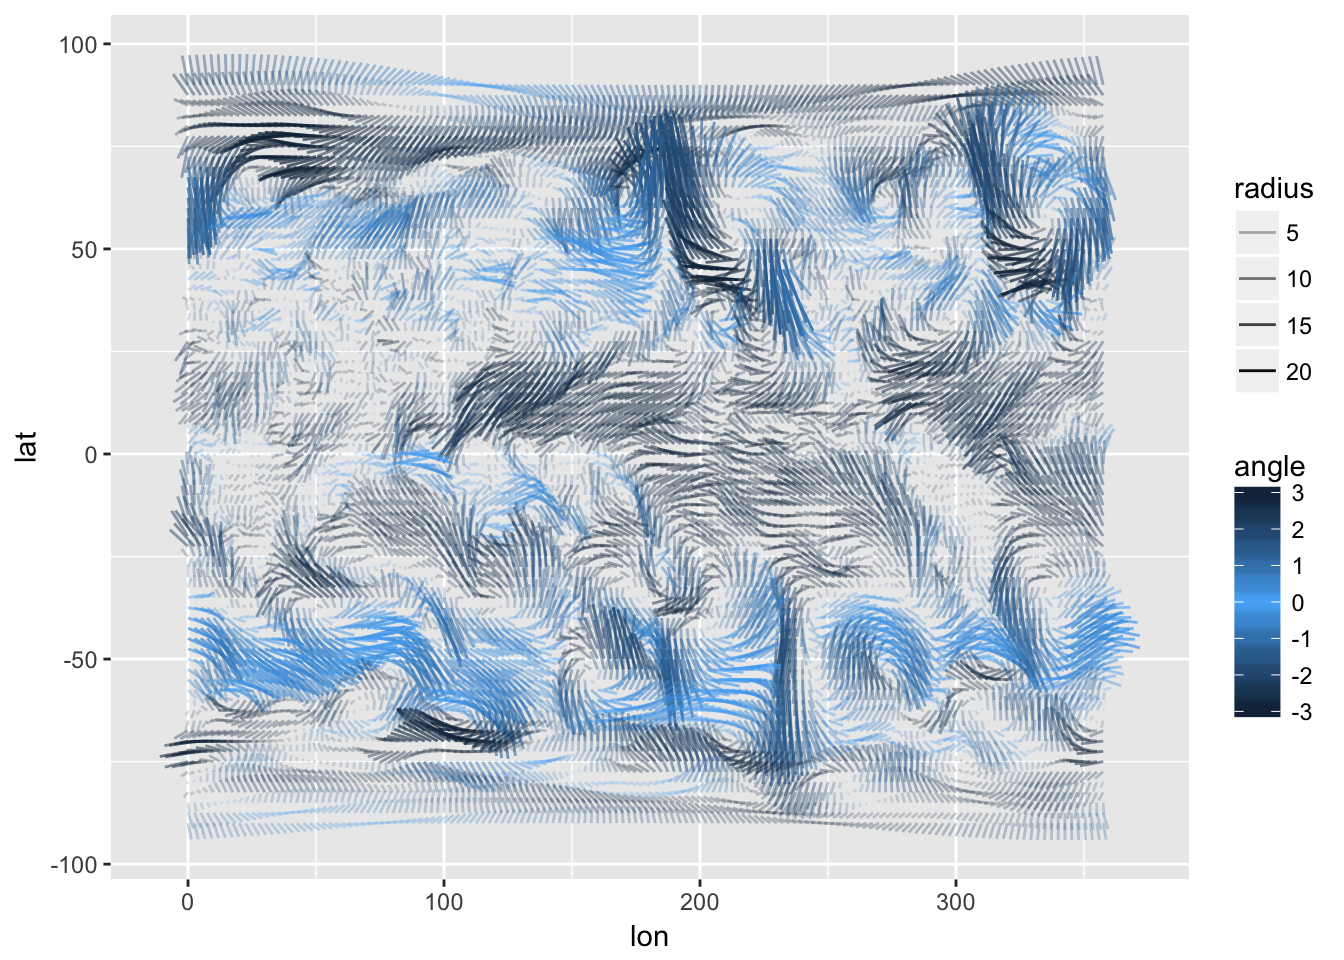
\includegraphics{07-geom_spoke_files/figure-latex/spoke-plot-1.pdf}

\section{maps}\label{maps}

\begin{verbatim}
install.packages("maps")
\end{verbatim}

Map data will help to provide some context to this wind figure. We'll
use \texttt{geom\_polygon} to plot the world centered on the Pacific
Ocean (\texttt{world2}) using the \texttt{map\_data()} function.

\begin{Shaded}
\begin{Highlighting}[]
\NormalTok{world <-}\StringTok{ }\KeywordTok{map_data}\NormalTok{(}\StringTok{"world2"}\NormalTok{)}
\NormalTok{wind %>%}
\StringTok{  }\KeywordTok{filter}\NormalTok{(time ==}\StringTok{ }\KeywordTok{as.POSIXct}\NormalTok{(}\StringTok{"2017-01-01"}\NormalTok{, }\DataTypeTok{tz =} \StringTok{"GMT"}\NormalTok{)) %>%}
\StringTok{  }\KeywordTok{ggplot}\NormalTok{(}\KeywordTok{aes}\NormalTok{(lon, lat)) +}
\StringTok{  }\KeywordTok{geom_polygon}\NormalTok{(}\DataTypeTok{data =} \NormalTok{world, }\KeywordTok{aes}\NormalTok{(}\DataTypeTok{x=}\NormalTok{long, }\DataTypeTok{y =} \NormalTok{lat, }\DataTypeTok{group =} \NormalTok{group), }\DataTypeTok{color =} \StringTok{"green"}\NormalTok{, }\DataTypeTok{fill =} \OtherTok{NA}\NormalTok{) +}\StringTok{ }
\StringTok{  }\KeywordTok{coord_fixed}\NormalTok{(}\DecValTok{1}\NormalTok{) +}
\StringTok{  }\KeywordTok{geom_spoke}\NormalTok{(}\KeywordTok{aes}\NormalTok{(}\DataTypeTok{angle =} \NormalTok{angle, }\DataTypeTok{radius =} \NormalTok{radius, }\DataTypeTok{alpha =} \NormalTok{radius, }\DataTypeTok{color =} \NormalTok{angle)) +}
\StringTok{  }\KeywordTok{scale_color_gradient2}\NormalTok{(}\DataTypeTok{low =} \StringTok{"#132B43"}\NormalTok{, }\DataTypeTok{mid =} \StringTok{"#56B1F7"}\NormalTok{, }\DataTypeTok{high =} \StringTok{"#132B43"}\NormalTok{) +}
\StringTok{  }\KeywordTok{theme_minimal}\NormalTok{()}
\end{Highlighting}
\end{Shaded}

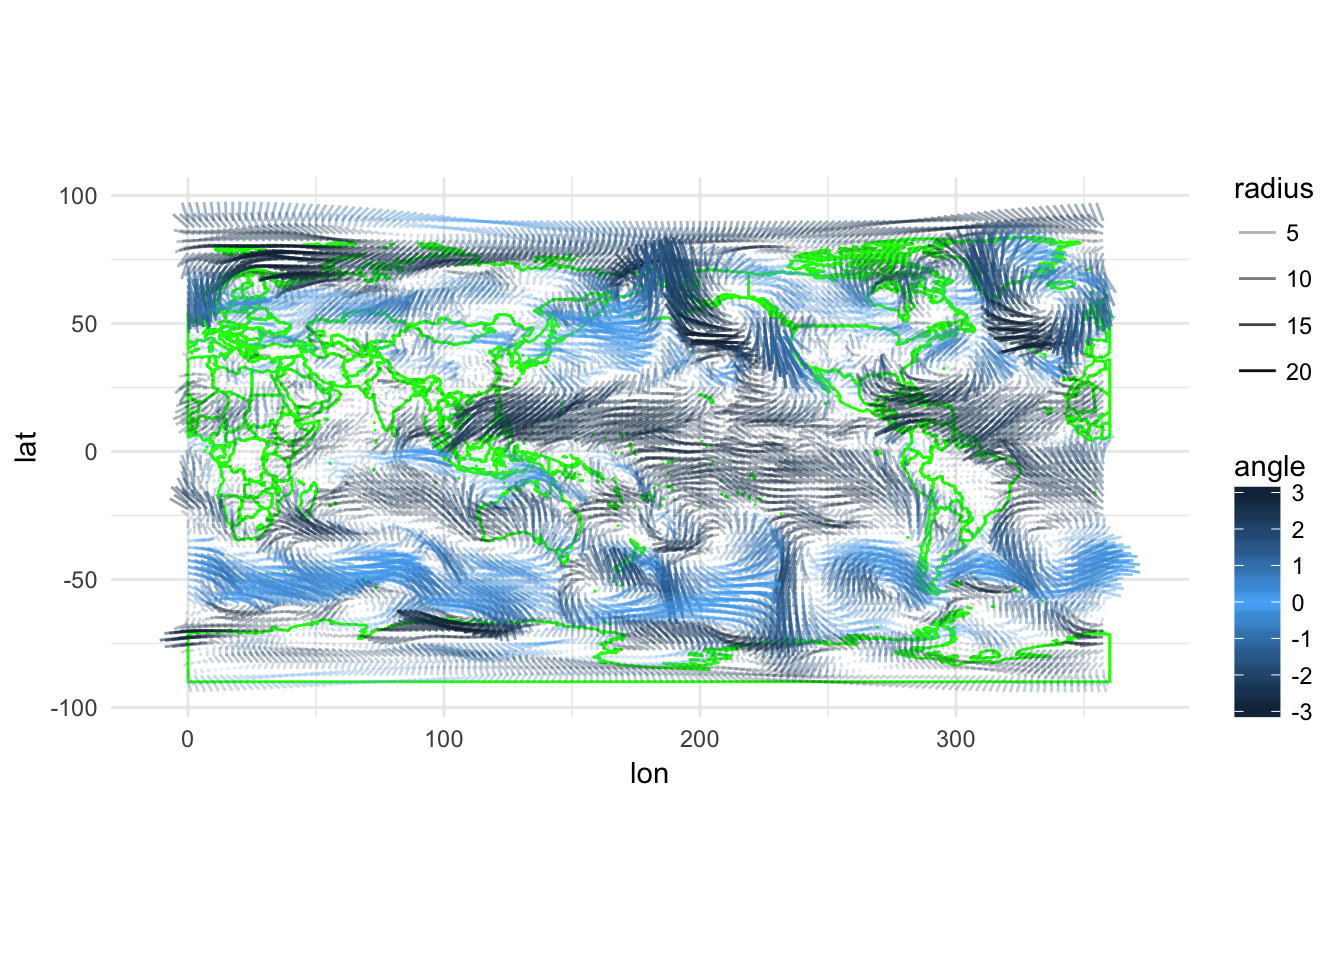
\includegraphics{07-geom_spoke_files/figure-latex/spoke-map-1.pdf}

\section{gganimate}\label{gganimate}

The \texttt{gganimate} package lets us animate the above chart. If you
want to be able to save animations as an mp4, you will need install
\texttt{ffmpeg} (\url{https://www.ffmpeg.org/download.html}). If you are
running macOS, you will need also need ImageMagick
(\url{http://www.imagemagick.org/script/binary-releases.php\#macosx}).

You can install \texttt{gganimate} with \texttt{devtools}:

\begin{verbatim}
devtools::install_github("dgrtwo/gganimate")
\end{verbatim}

\begin{Shaded}
\begin{Highlighting}[]
\KeywordTok{library}\NormalTok{(gganimate)}
\NormalTok{f <-}\StringTok{ }\NormalTok{wind %>%}
\StringTok{  }\KeywordTok{ggplot}\NormalTok{(}\KeywordTok{aes}\NormalTok{(lon, lat)) +}
\StringTok{  }\KeywordTok{geom_polygon}\NormalTok{(}\DataTypeTok{data =} \NormalTok{world, }\KeywordTok{aes}\NormalTok{(}\DataTypeTok{x=}\NormalTok{long, }\DataTypeTok{y =} \NormalTok{lat, }\DataTypeTok{group =} \NormalTok{group), }\DataTypeTok{color =} \StringTok{"green"}\NormalTok{, }\DataTypeTok{fill =} \OtherTok{NA}\NormalTok{) +}\StringTok{ }
\StringTok{  }\KeywordTok{coord_fixed}\NormalTok{(}\DecValTok{1}\NormalTok{) +}
\StringTok{  }\KeywordTok{geom_spoke}\NormalTok{(}\KeywordTok{aes}\NormalTok{(}\DataTypeTok{angle =} \NormalTok{angle, }\DataTypeTok{radius =} \NormalTok{radius, }\DataTypeTok{alpha =} \NormalTok{radius, }\DataTypeTok{color =} \NormalTok{angle, }\DataTypeTok{frame =} \NormalTok{time)) +}
\StringTok{  }\KeywordTok{scale_color_gradient2}\NormalTok{(}\DataTypeTok{low =} \StringTok{"#132B43"}\NormalTok{, }\DataTypeTok{mid =} \StringTok{"#56B1F7"}\NormalTok{, }\DataTypeTok{high =} \StringTok{"#132B43"}\NormalTok{) +}
\StringTok{  }\KeywordTok{theme_minimal}\NormalTok{()}
\KeywordTok{gganimate}\NormalTok{(f)}
\end{Highlighting}
\end{Shaded}

\section{glyphs}\label{glyphs}

\texttt{glyphs} provide another useful way of analyzing spatial data
with a time dimesion. This shows a tiny line charts representing the
north-south component of the wind at each longitude/latitude
combination.

\begin{verbatim}
library(GGally)
wind$day <- as.numeric(julian(wind$time, as.POSIXct("2017-01-01", tz = "GMT")))
wind$day_flip <- -wind$day
vwnd_gly <- glyphs(wind, "lon", "day", "lat", "vwnd", height=2.5)
uwnd_gly <- glyphs(wind, "lon", "day", "lat", "uwnd", height=2.5)

ggplot(vwnd_gly, aes(gx, gy, group = gid)) +
  add_ref_lines(vwnd_gly, color = "grey90") +
  add_ref_boxes(vwnd_gly, color = "grey90") +
  geom_path() +
  theme_bw() +
  labs(x = "", y = "")
\end{verbatim}

\begin{figure}[htbp]
\centering
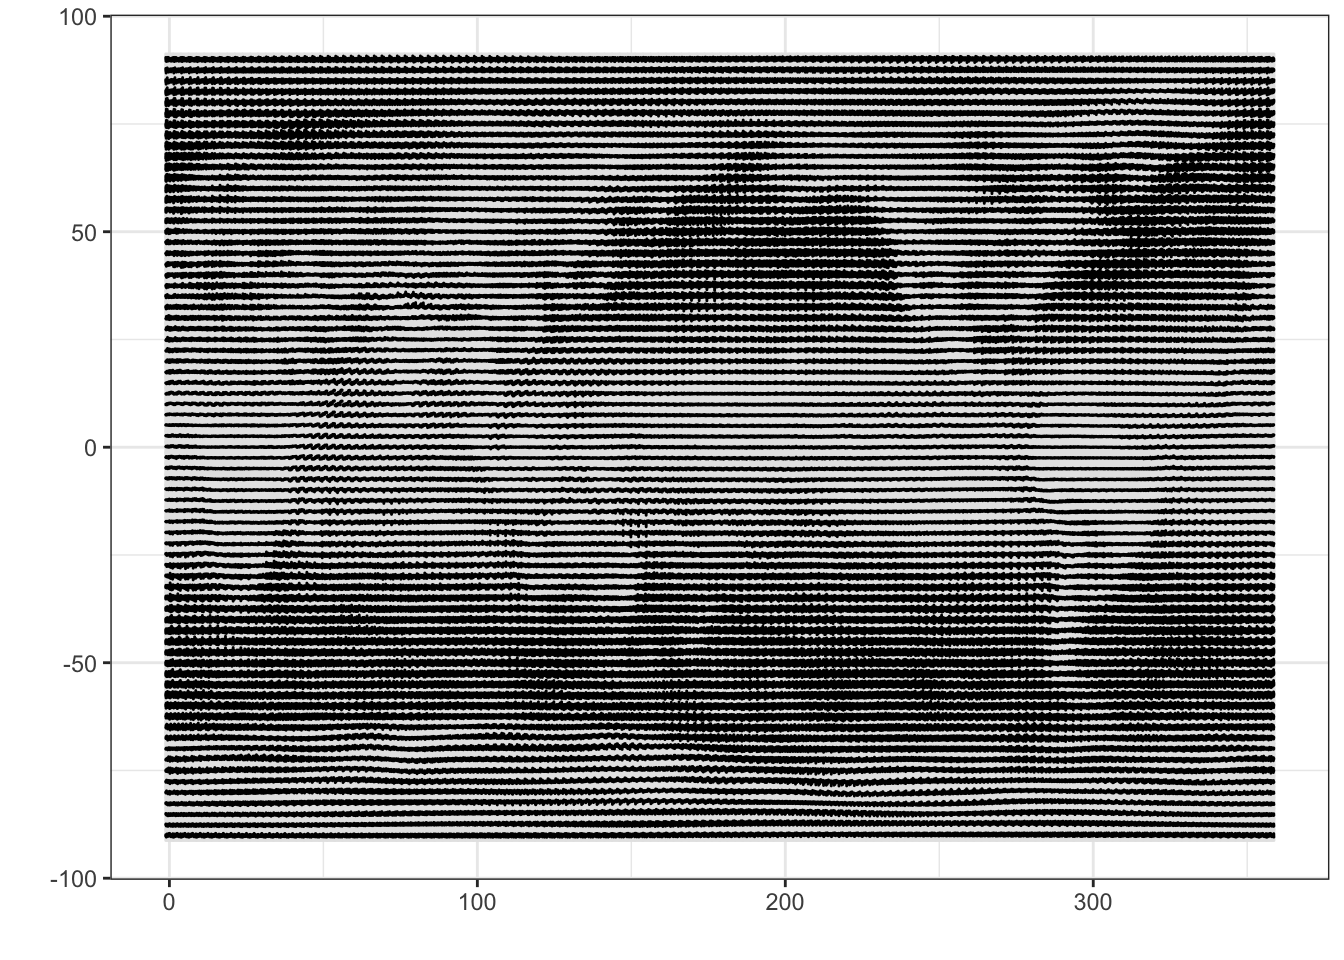
\includegraphics{fig/spoke-glyphs-1.png}
\caption{}
\end{figure}

Let's focus in on just the continental US:

\begin{Shaded}
\begin{Highlighting}[]
\KeywordTok{library}\NormalTok{(GGally)}

\NormalTok{usa <-}\StringTok{ }\KeywordTok{map_data}\NormalTok{(}\StringTok{"usa"}\NormalTok{)}
\NormalTok{usa_long_range <-}\StringTok{ }\KeywordTok{range}\NormalTok{(usa$long)}
\NormalTok{usa_lat_range <-}\StringTok{ }\KeywordTok{range}\NormalTok{(usa$lat)}

\NormalTok{usa_wind <-}\StringTok{ }\NormalTok{wind %>%}
\StringTok{  }\KeywordTok{filter}\NormalTok{(lon >=}\StringTok{ }\NormalTok{(usa_long_range[}\DecValTok{1}\NormalTok{] %%}\StringTok{ }\DecValTok{360}\NormalTok{) &}\StringTok{ }\NormalTok{lon <=}\StringTok{ }\NormalTok{(usa_long_range[}\DecValTok{2}\NormalTok{] %%}\StringTok{ }\DecValTok{360}\NormalTok{) &}
\StringTok{           }\NormalTok{lat >=}\StringTok{ }\NormalTok{usa_lat_range[}\DecValTok{1}\NormalTok{] &}\StringTok{ }\NormalTok{lat <=}\StringTok{ }\NormalTok{usa_lat_range[}\DecValTok{2}\NormalTok{])}
\NormalTok{usa_wind$day <-}\StringTok{ }\KeywordTok{as.numeric}\NormalTok{(}\KeywordTok{julian}\NormalTok{(usa_wind$time, }\KeywordTok{as.POSIXct}\NormalTok{(}\StringTok{"2017-01-01"}\NormalTok{, }\DataTypeTok{tz =} \StringTok{"GMT"}\NormalTok{)))}
\NormalTok{usa_wind$day_flip <-}\StringTok{ }\NormalTok{-usa_wind$day}
\NormalTok{usa_vwnd_gly <-}\StringTok{ }\KeywordTok{glyphs}\NormalTok{(usa_wind, }\StringTok{"lon"}\NormalTok{, }\StringTok{"day"}\NormalTok{, }\StringTok{"lat"}\NormalTok{, }\StringTok{"vwnd"}\NormalTok{, }\DataTypeTok{height=}\FloatTok{2.5}\NormalTok{)}
\NormalTok{usa_uwnd_gly <-}\StringTok{ }\KeywordTok{glyphs}\NormalTok{(usa_wind, }\StringTok{"lon"}\NormalTok{, }\StringTok{"uwnd"}\NormalTok{, }\StringTok{"lat"}\NormalTok{, }\StringTok{"day_flip"}\NormalTok{, }\DataTypeTok{height=}\FloatTok{2.5}\NormalTok{)}

\KeywordTok{ggplot}\NormalTok{(usa_vwnd_gly, }\KeywordTok{aes}\NormalTok{(gx, gy, }\DataTypeTok{group =} \NormalTok{gid)) +}
\StringTok{  }\KeywordTok{geom_polygon}\NormalTok{(}\DataTypeTok{data =} \NormalTok{usa, }\KeywordTok{aes}\NormalTok{(}\DataTypeTok{x =} \NormalTok{long %%}\StringTok{ }\DecValTok{360}\NormalTok{, }\DataTypeTok{y =} \NormalTok{lat %%}\StringTok{ }\DecValTok{360}\NormalTok{, }\DataTypeTok{group =} \NormalTok{group), }\DataTypeTok{fill =} \StringTok{"grey60"}\NormalTok{) +}
\StringTok{  }\KeywordTok{add_ref_lines}\NormalTok{(usa_vwnd_gly, }\DataTypeTok{color =} \StringTok{"grey90"}\NormalTok{) +}
\StringTok{  }\KeywordTok{add_ref_boxes}\NormalTok{(usa_vwnd_gly, }\DataTypeTok{color =} \StringTok{"grey90"}\NormalTok{) +}
\StringTok{  }\KeywordTok{geom_path}\NormalTok{(}\DataTypeTok{alpha =} \FloatTok{0.9}\NormalTok{) +}
\StringTok{  }\KeywordTok{theme_bw}\NormalTok{() +}
\StringTok{  }\KeywordTok{labs}\NormalTok{(}\DataTypeTok{x =} \StringTok{""}\NormalTok{, }\DataTypeTok{y =} \StringTok{""}\NormalTok{, }\DataTypeTok{title =} \StringTok{"North-South"}\NormalTok{)}
\KeywordTok{ggplot}\NormalTok{(usa_uwnd_gly, }\KeywordTok{aes}\NormalTok{(gx, gy, }\DataTypeTok{group =} \NormalTok{gid)) +}
\StringTok{  }\KeywordTok{geom_polygon}\NormalTok{(}\DataTypeTok{data =} \NormalTok{usa, }\KeywordTok{aes}\NormalTok{(}\DataTypeTok{x =} \NormalTok{long %%}\StringTok{ }\DecValTok{360}\NormalTok{, }\DataTypeTok{y =} \NormalTok{lat %%}\StringTok{ }\DecValTok{360}\NormalTok{, }\DataTypeTok{group =} \NormalTok{group), }\DataTypeTok{fill =} \StringTok{"grey60"}\NormalTok{) +}
\StringTok{  }\KeywordTok{add_ref_lines}\NormalTok{(usa_uwnd_gly, }\DataTypeTok{color =} \StringTok{"grey90"}\NormalTok{) +}
\StringTok{  }\KeywordTok{add_ref_boxes}\NormalTok{(usa_uwnd_gly, }\DataTypeTok{color =} \StringTok{"grey90"}\NormalTok{) +}
\StringTok{  }\KeywordTok{geom_path}\NormalTok{(}\DataTypeTok{alpha =} \FloatTok{0.9}\NormalTok{) +}
\StringTok{  }\KeywordTok{theme_bw}\NormalTok{() +}
\StringTok{  }\KeywordTok{labs}\NormalTok{(}\DataTypeTok{x =} \StringTok{""}\NormalTok{, }\DataTypeTok{y =} \StringTok{""}\NormalTok{, }\DataTypeTok{title =} \StringTok{"East-West"}\NormalTok{)}
\end{Highlighting}
\end{Shaded}

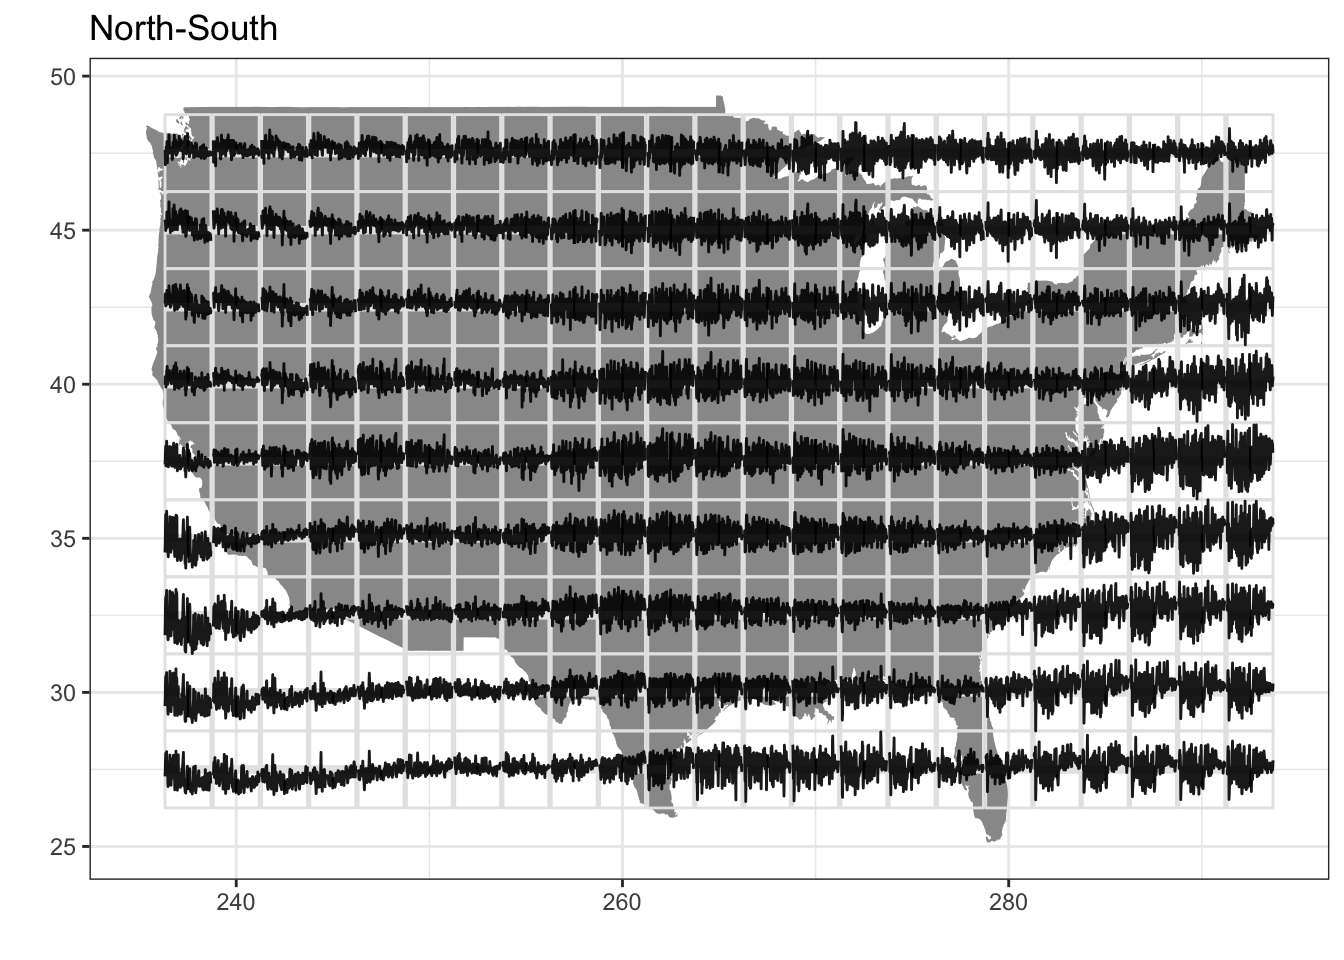
\includegraphics{07-geom_spoke_files/figure-latex/spoke-glyphs-zoom-1.pdf}
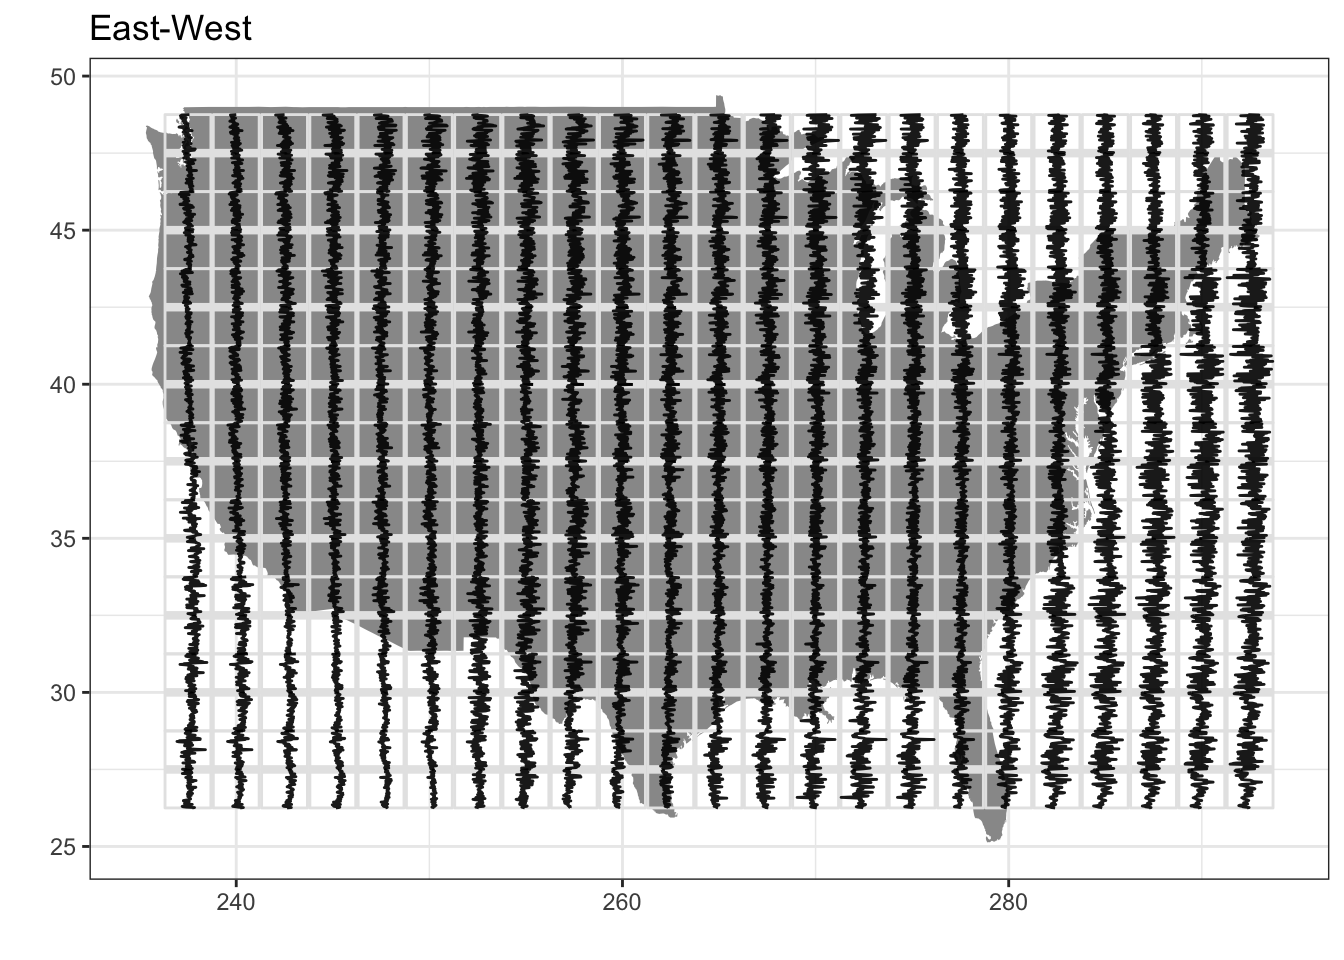
\includegraphics{07-geom_spoke_files/figure-latex/spoke-glyphs-zoom-2.pdf}

\section{Assignment}\label{assignment-6}

Create heatmaps of \texttt{uwnd} and \texttt{vwnd} values on March 31,
2017. Each heatmap should be 90 degrees longitude by 90 degrees
lattitude. Hint: Use \texttt{facet\_grid} and create two new variables
to help with faceting. The plot should end up being 5 facets wide by 3
facets tall.

\hypertarget{area-and-ribbons}{\chapter{geom\_area and
geom\_ribbon}\label{area-and-ribbons}}

\section{Data}\label{data-5}

The US Bureau of Labor Statistics (BLS) conducts the American Time Use
Survey (ATUS). You can download the text form of the ATUS by going to
the \href{https://www.bls.gov/data/}{BLS data page}, finding the section
labelled Spending \& Time Use, then clicking on the ``Text Files''
button on the row for the ATUS. Or by using the following link:

\url{https://download.bls.gov/pub/time.series/tu/}

\subsection{Downloading a file from the
internet}\label{downloading-a-file-from-the-internet}

While you can manually download the files from the above URL,
\texttt{download.file()} lets you download files from within R. The
first argument is the URL of the resource you want to download. The
second argument is the destination for the file. The following requests
will require you to create the \texttt{tu} folder.

\begin{verbatim}
download.file("https://download.bls.gov/pub/time.series/tu/tu.txt", "data/tu/tu.txt")
download.file("https://download.bls.gov/pub/time.series/tu/tu.series", "data/tu/tu.series")
download.file("https://download.bls.gov/pub/time.series/tu/tu.data.0.Current", "data/tu/tu.data.0.Current")
\end{verbatim}

The file \texttt{tu.txt} contains the documentation for the time use
(tu) survey data. Section 2 of that file provides descriptions of each
of the files in the \texttt{pub/time.series/tu} folder. From that list
we can see that \texttt{tu.series} will give us a list of the available
series.

\begin{Shaded}
\begin{Highlighting}[]
\KeywordTok{library}\NormalTok{(readr)}
\NormalTok{series_defn <-}\StringTok{ }\KeywordTok{read_tsv}\NormalTok{(}\StringTok{"data/tu/tu.series"}\NormalTok{)}
\NormalTok{series_defn}
\end{Highlighting}
\end{Shaded}

\begin{verbatim}
## # A tibble: 85,277 x 43
##             series_id seasonal stattype_code datays_code sex_code
##                 <chr>    <chr>         <int>       <chr>    <int>
##  1 TUU10100AA01000007        U         10100          01        0
##  2 TUU10100AA01000013        U         10100          01        0
##  3 TUU10100AA01000014        U         10100          01        0
##  4 TUU10100AA01000015        U         10100          01        0
##  5 TUU10100AA01000018        U         10100          01        0
##  6 TUU10100AA01000019        U         10100          01        0
##  7 TUU10100AA01000025        U         10100          01        0
##  8 TUU10100AA01000035        U         10100          01        0
##  9 TUU10100AA01000036        U         10100          01        0
## 10 TUU10100AA01000037        U         10100          01        0
## # ... with 85,267 more rows, and 38 more variables: region_code <chr>,
## #   lfstat_code <chr>, educ_code <chr>, maritlstat_code <chr>,
## #   age_code <chr>, orig_code <chr>, race_code <chr>, mjcow_code <chr>,
## #   nmet_code <int>, where_code <chr>, sjmj_code <int>,
## #   timeday_code <chr>, actcode_code <chr>, industry_code <chr>,
## #   occ_code <chr>, prhhchild_code <chr>, earn_code <chr>,
## #   disability_code <chr>, who_code <chr>, hhnscc03_code <chr>,
## #   schenr_code <int>, prownhhchild_code <chr>, work_code <int>,
## #   elnum_code <chr>, ecage_code <chr>, elfreq_code <int>,
## #   eldur_code <chr>, elwho_code <chr>, ecytd_code <int>,
## #   elder_code <int>, lfstatw_code <chr>, pertype_code <chr>,
## #   series_title <chr>, footnote_codes <chr>, begin_year <int>,
## #   begin_period <chr>, end_year <int>, end_period <chr>
\end{verbatim}

There is a lot here to process. The columns we care most about for now
are \texttt{series\_id} and \texttt{series\_title}. Using
\texttt{select()} from the \texttt{dplyr} library, we can show just the
columns we care about.

\begin{Shaded}
\begin{Highlighting}[]
\KeywordTok{library}\NormalTok{(dplyr)}
\NormalTok{series_defn %>%}
\StringTok{  }\KeywordTok{select}\NormalTok{(series_id, series_title)}
\end{Highlighting}
\end{Shaded}

\begin{verbatim}
## # A tibble: 85,277 x 2
##             series_id
##                 <chr>
##  1 TUU10100AA01000007
##  2 TUU10100AA01000013
##  3 TUU10100AA01000014
##  4 TUU10100AA01000015
##  5 TUU10100AA01000018
##  6 TUU10100AA01000019
##  7 TUU10100AA01000025
##  8 TUU10100AA01000035
##  9 TUU10100AA01000036
## 10 TUU10100AA01000037
## # ... with 85,267 more rows, and 1 more variables: series_title <chr>
\end{verbatim}

\subsection{Pairing down the list of
variables}\label{pairing-down-the-list-of-variables}

Let's look for variables on sleep, work, and leisure:

\begin{Shaded}
\begin{Highlighting}[]
\NormalTok{series_defn %>%}
\StringTok{  }\KeywordTok{select}\NormalTok{(series_title) %>%}
\StringTok{  }\KeywordTok{filter}\NormalTok{(}\KeywordTok{grepl}\NormalTok{(}\StringTok{"sleep"}\NormalTok{, series_title, }\DataTypeTok{ignore.case =} \OtherTok{TRUE}\NormalTok{))}
\end{Highlighting}
\end{Shaded}

\begin{verbatim}
## # A tibble: 1,310 x 1
##                                                                   series_title
##                                                                          <chr>
##  1                                                  Avg hrs per day - Sleeping
##  2                       Avg hrs per day - Sleeping, Weekend days and holidays
##  3                             Avg hrs per day - Sleeping, Nonholiday weekdays
##  4                                        Avg hrs per day - Sleeping, Employed
##  5             Avg hrs per day - Sleeping, Weekend days and holidays, Employed
##  6                   Avg hrs per day - Sleeping, Nonholiday weekdays, Employed
##  7                        Avg hrs per day - Sleeping, Employed, on days worked
##  8 Avg hrs per day - Sleeping, Weekend days and holidays, Employed, on days wo
##  9   Avg hrs per day - Sleeping, Nonholiday weekdays, Employed, on days worked
## 10                              Avg hrs per day - Sleeping, Employed full time
## # ... with 1,300 more rows
\end{verbatim}

Since this simple search returns a ton of results, let's further filter
by `employed' and `per day':

\begin{Shaded}
\begin{Highlighting}[]
\NormalTok{series_defn %>%}
\StringTok{  }\KeywordTok{select}\NormalTok{(series_title) %>%}
\StringTok{  }\KeywordTok{filter}\NormalTok{(}\KeywordTok{grepl}\NormalTok{(}\StringTok{"per day.*sleep.*employed"}\NormalTok{, series_title, }\DataTypeTok{ignore.case =} \OtherTok{TRUE}\NormalTok{))}
\end{Highlighting}
\end{Shaded}

\begin{verbatim}
## # A tibble: 154 x 1
##                                                                   series_title
##                                                                          <chr>
##  1                                        Avg hrs per day - Sleeping, Employed
##  2             Avg hrs per day - Sleeping, Weekend days and holidays, Employed
##  3                   Avg hrs per day - Sleeping, Nonholiday weekdays, Employed
##  4                        Avg hrs per day - Sleeping, Employed, on days worked
##  5 Avg hrs per day - Sleeping, Weekend days and holidays, Employed, on days wo
##  6   Avg hrs per day - Sleeping, Nonholiday weekdays, Employed, on days worked
##  7                              Avg hrs per day - Sleeping, Employed full time
##  8   Avg hrs per day - Sleeping, Weekend days and holidays, Employed full time
##  9         Avg hrs per day - Sleeping, Nonholiday weekdays, Employed full time
## 10              Avg hrs per day - Sleeping, Employed full time, on days worked
## # ... with 144 more rows
\end{verbatim}

Now let's filter further by `employed full time', `nonholiday weekdays',
and `on days worked':

\begin{Shaded}
\begin{Highlighting}[]
\NormalTok{series_defn %>%}
\StringTok{  }\KeywordTok{select}\NormalTok{(series_title) %>%}
\StringTok{  }\KeywordTok{filter}\NormalTok{(}\KeywordTok{grepl}\NormalTok{(}\StringTok{"per day.*sleep.*nonholiday weekdays.*employed full time.*on days worked"}\NormalTok{, series_title, }\DataTypeTok{ignore.case =} \OtherTok{TRUE}\NormalTok{))}
\end{Highlighting}
\end{Shaded}

\begin{verbatim}
## # A tibble: 6 x 1
##                                                                  series_title
##                                                                         <chr>
## 1 Avg hrs per day - Sleeping, Nonholiday weekdays, Employed full time, on day
## 2 Avg hrs per day - Sleeping, Nonholiday weekdays, Employed full time, on day
## 3 Avg hrs per day - Sleeping, Nonholiday weekdays, Employed full time, on day
## 4 Avg hrs per day for participants - Sleeping, Nonholiday weekdays, Employed 
## 5 Avg hrs per day for participants - Sleeping, Nonholiday weekdays, Employed 
## 6 Avg hrs per day for participants - Sleeping, Nonholiday weekdays, Employed
\end{verbatim}

Finally, let's filter that to exclude the `participants only' group and
only get the Men/Women values (not the combined totals):

\begin{Shaded}
\begin{Highlighting}[]
\NormalTok{series_defn %>%}
\StringTok{  }\KeywordTok{select}\NormalTok{(series_title) %>%}
\StringTok{  }\KeywordTok{filter}\NormalTok{(}\KeywordTok{grepl}\NormalTok{(}\StringTok{"per day -.*sleep.*nonholiday weekdays.*employed full time.*on days worked,"}\NormalTok{, series_title, }\DataTypeTok{ignore.case =} \OtherTok{TRUE}\NormalTok{))}
\end{Highlighting}
\end{Shaded}

\begin{verbatim}
## # A tibble: 2 x 1
##                                                                  series_title
##                                                                         <chr>
## 1 Avg hrs per day - Sleeping, Nonholiday weekdays, Employed full time, on day
## 2 Avg hrs per day - Sleeping, Nonholiday weekdays, Employed full time, on day
\end{verbatim}

\subsection{Adding more activity
categories}\label{adding-more-activity-categories}

Now let's add `work' and `leisure' to our search:

\begin{Shaded}
\begin{Highlighting}[]
\NormalTok{activity <-}\StringTok{ }\NormalTok{series_defn %>%}
\StringTok{  }\KeywordTok{select}\NormalTok{(series_id, series_title) %>%}
\StringTok{  }\KeywordTok{filter}\NormalTok{(}\KeywordTok{grepl}\NormalTok{(}\StringTok{"per day -.*(sleep|work|leisure).*nonholiday weekdays.*employed full time.*on days worked,"}\NormalTok{, series_title, }\DataTypeTok{ignore.case =} \OtherTok{TRUE}\NormalTok{))}
\NormalTok{activity}
\end{Highlighting}
\end{Shaded}

\begin{verbatim}
## # A tibble: 26 x 2
##             series_id
##                 <chr>
##  1 TUU10101AA01000344
##  2 TUU10101AA01000423
##  3 TUU10101AA01000962
##  4 TUU10101AA01001041
##  5 TUU10101AA01003012
##  6 TUU10101AA01003097
##  7 TUU10101AA01003307
##  8 TUU10101AA01003378
##  9 TUU10101AA01003947
## 10 TUU10101AA01004011
## # ... with 16 more rows, and 1 more variables: series_title <chr>
\end{verbatim}

Now we should create a variable that codes each of these as either work,
sleep, or leisure:

\begin{Shaded}
\begin{Highlighting}[]
\NormalTok{activity <-}\StringTok{ }\NormalTok{activity %>%}
\StringTok{  }\KeywordTok{mutate}\NormalTok{(}
    \DataTypeTok{activity_type =} \KeywordTok{case_when}\NormalTok{(}
      \KeywordTok{grepl}\NormalTok{(}\StringTok{"leisure"}\NormalTok{, activity$series_title, }\DataTypeTok{ignore.case =} \OtherTok{TRUE}\NormalTok{) ~}\StringTok{ "Leisure"}\NormalTok{,}
      \KeywordTok{grepl}\NormalTok{(}\StringTok{"sleep"}\NormalTok{, activity$series_title, }\DataTypeTok{ignore.case =} \OtherTok{TRUE}\NormalTok{) ~}\StringTok{ "Sleep"}\NormalTok{,}
      \OtherTok{TRUE} \NormalTok{~}\StringTok{ "Work"}
    \NormalTok{), }
    \DataTypeTok{sex =} \KeywordTok{ifelse}\NormalTok{(}\KeywordTok{grepl}\NormalTok{(}\StringTok{"Men"}\NormalTok{, series_title), }\StringTok{"Men"}\NormalTok{, }\StringTok{"Women"}\NormalTok{)}
  \NormalTok{)}
\NormalTok{activity}
\end{Highlighting}
\end{Shaded}

\begin{verbatim}
## # A tibble: 26 x 4
##             series_id
##                 <chr>
##  1 TUU10101AA01000344
##  2 TUU10101AA01000423
##  3 TUU10101AA01000962
##  4 TUU10101AA01001041
##  5 TUU10101AA01003012
##  6 TUU10101AA01003097
##  7 TUU10101AA01003307
##  8 TUU10101AA01003378
##  9 TUU10101AA01003947
## 10 TUU10101AA01004011
## # ... with 16 more rows, and 3 more variables: series_title <chr>,
## #   activity_type <chr>, sex <chr>
\end{verbatim}

Now we can join the activity data.frame with the current data and create
time series of each activity type we created.

\begin{Shaded}
\begin{Highlighting}[]
\NormalTok{data <-}\StringTok{ }\KeywordTok{read_tsv}\NormalTok{(}\StringTok{"data/tu/tu.data.0.Current"}\NormalTok{)}
\NormalTok{data <-}\StringTok{ }\NormalTok{data %>%}
\StringTok{  }\KeywordTok{inner_join}\NormalTok{(activity) %>%}
\StringTok{  }\KeywordTok{group_by}\NormalTok{(year, sex, activity_type) %>%}
\StringTok{  }\KeywordTok{summarize}\NormalTok{(}\DataTypeTok{hours =} \KeywordTok{sum}\NormalTok{(}\KeywordTok{as.numeric}\NormalTok{(value), }\DataTypeTok{na.rm =} \OtherTok{TRUE}\NormalTok{))}
\NormalTok{data}
\end{Highlighting}
\end{Shaded}

\begin{verbatim}
## # A tibble: 84 x 4
## # Groups:   year, sex [?]
##     year   sex activity_type hours
##    <int> <chr>         <chr> <dbl>
##  1  2003   Men       Leisure  8.49
##  2  2003   Men         Sleep  7.46
##  3  2003   Men          Work 19.26
##  4  2003 Women       Leisure  7.02
##  5  2003 Women         Sleep  7.65
##  6  2003 Women          Work 17.87
##  7  2004   Men       Leisure  8.66
##  8  2004   Men         Sleep  7.49
##  9  2004   Men          Work 18.92
## 10  2004 Women       Leisure  7.34
## # ... with 74 more rows
\end{verbatim}

\section{geom\_area}\label{geom_area}

\texttt{geom\_area} is useful when components that naturally add to each
other:

\begin{Shaded}
\begin{Highlighting}[]
\KeywordTok{library}\NormalTok{(ggplot2)}
\KeywordTok{ggplot}\NormalTok{(data, }\KeywordTok{aes}\NormalTok{(year, hours, }\DataTypeTok{fill=} \NormalTok{activity_type)) +}\StringTok{ }\KeywordTok{geom_area}\NormalTok{() +}\StringTok{ }\KeywordTok{facet_wrap}\NormalTok{(~}\StringTok{ }\NormalTok{sex) }
\end{Highlighting}
\end{Shaded}

\includegraphics{08-area-and-ribbons_files/figure-latex/unnamed-chunk-11-1.pdf}

\section{geom\_ribbon}\label{geom_ribbon}

\begin{Shaded}
\begin{Highlighting}[]
\NormalTok{data %>%}
\StringTok{  }\KeywordTok{ggplot}\NormalTok{(}\KeywordTok{aes}\NormalTok{(}\DataTypeTok{x =} \NormalTok{year, }\DataTypeTok{group =} \NormalTok{sex, }\DataTypeTok{fill =} \NormalTok{activity_type)) +}\StringTok{ }
\StringTok{  }\KeywordTok{geom_ribbon}\NormalTok{(}\DataTypeTok{mapping =} \KeywordTok{aes}\NormalTok{(}\DataTypeTok{ymin =} \NormalTok{-hours *}\StringTok{ }\NormalTok{(sex ==}\StringTok{ "Women"}\NormalTok{), }\DataTypeTok{ymax =} \NormalTok{hours *}\StringTok{ }\NormalTok{(sex ==}\StringTok{ "Men"}\NormalTok{)), }\DataTypeTok{data =} \NormalTok{. %>%}\StringTok{ }\KeywordTok{filter}\NormalTok{(activity_type ==}\StringTok{ "Work"}\NormalTok{), }\DataTypeTok{alpha =} \FloatTok{0.5}\NormalTok{) +}
\StringTok{  }\KeywordTok{geom_ribbon}\NormalTok{(}\DataTypeTok{mapping =} \KeywordTok{aes}\NormalTok{(}\DataTypeTok{ymin =} \NormalTok{-hours *}\StringTok{ }\NormalTok{(sex ==}\StringTok{ "Women"}\NormalTok{), }\DataTypeTok{ymax =} \NormalTok{hours *}\StringTok{ }\NormalTok{(sex ==}\StringTok{ "Men"}\NormalTok{)), }\DataTypeTok{data =} \NormalTok{. %>%}\StringTok{ }\KeywordTok{filter}\NormalTok{(activity_type ==}\StringTok{ "Leisure"}\NormalTok{), }\DataTypeTok{alpha =} \FloatTok{0.5}\NormalTok{) +}
\StringTok{  }\KeywordTok{geom_ribbon}\NormalTok{(}\DataTypeTok{mapping =} \KeywordTok{aes}\NormalTok{(}\DataTypeTok{ymin =} \NormalTok{-hours *}\StringTok{ }\NormalTok{(sex ==}\StringTok{ "Women"}\NormalTok{), }\DataTypeTok{ymax =} \NormalTok{hours *}\StringTok{ }\NormalTok{(sex ==}\StringTok{ "Men"}\NormalTok{)), }\DataTypeTok{data =} \NormalTok{. %>%}\StringTok{ }\KeywordTok{filter}\NormalTok{(activity_type ==}\StringTok{ "Sleep"}\NormalTok{), }\DataTypeTok{alpha =} \FloatTok{0.5}\NormalTok{) +}
\StringTok{  }\KeywordTok{scale_y_continuous}\NormalTok{(}
    \DataTypeTok{name =} \StringTok{"Average hours per work day (Fully Employed)"}\NormalTok{,}
    \DataTypeTok{breaks =} \KeywordTok{c}\NormalTok{(-}\DecValTok{20}\NormalTok{, -}\DecValTok{10}\NormalTok{, }\DecValTok{0}\NormalTok{, }\DecValTok{10}\NormalTok{, }\DecValTok{20}\NormalTok{),}
    \DataTypeTok{labels =} \KeywordTok{c}\NormalTok{(}\StringTok{"Women 20 hrs"}\NormalTok{, }\StringTok{"10 hrs"}\NormalTok{, }\StringTok{"0 hrs"}\NormalTok{, }\StringTok{"10 hrs"}\NormalTok{, }\StringTok{"Men 20 hrs"}\NormalTok{),}
    \DataTypeTok{limits =} \KeywordTok{c}\NormalTok{(-}\DecValTok{20}\NormalTok{, }\DecValTok{20}\NormalTok{)}
    \NormalTok{)}
\end{Highlighting}
\end{Shaded}

\includegraphics{08-area-and-ribbons_files/figure-latex/unnamed-chunk-12-1.pdf}

\section{Assignment}\label{assignment-7}

Plot leisure computer use over time using separate lines for men and
women. The y axis should display the amount of use in minutes. The plot
should look like the following image (the aspect ratio can be
different).

\begin{figure}[htbp]
\centering
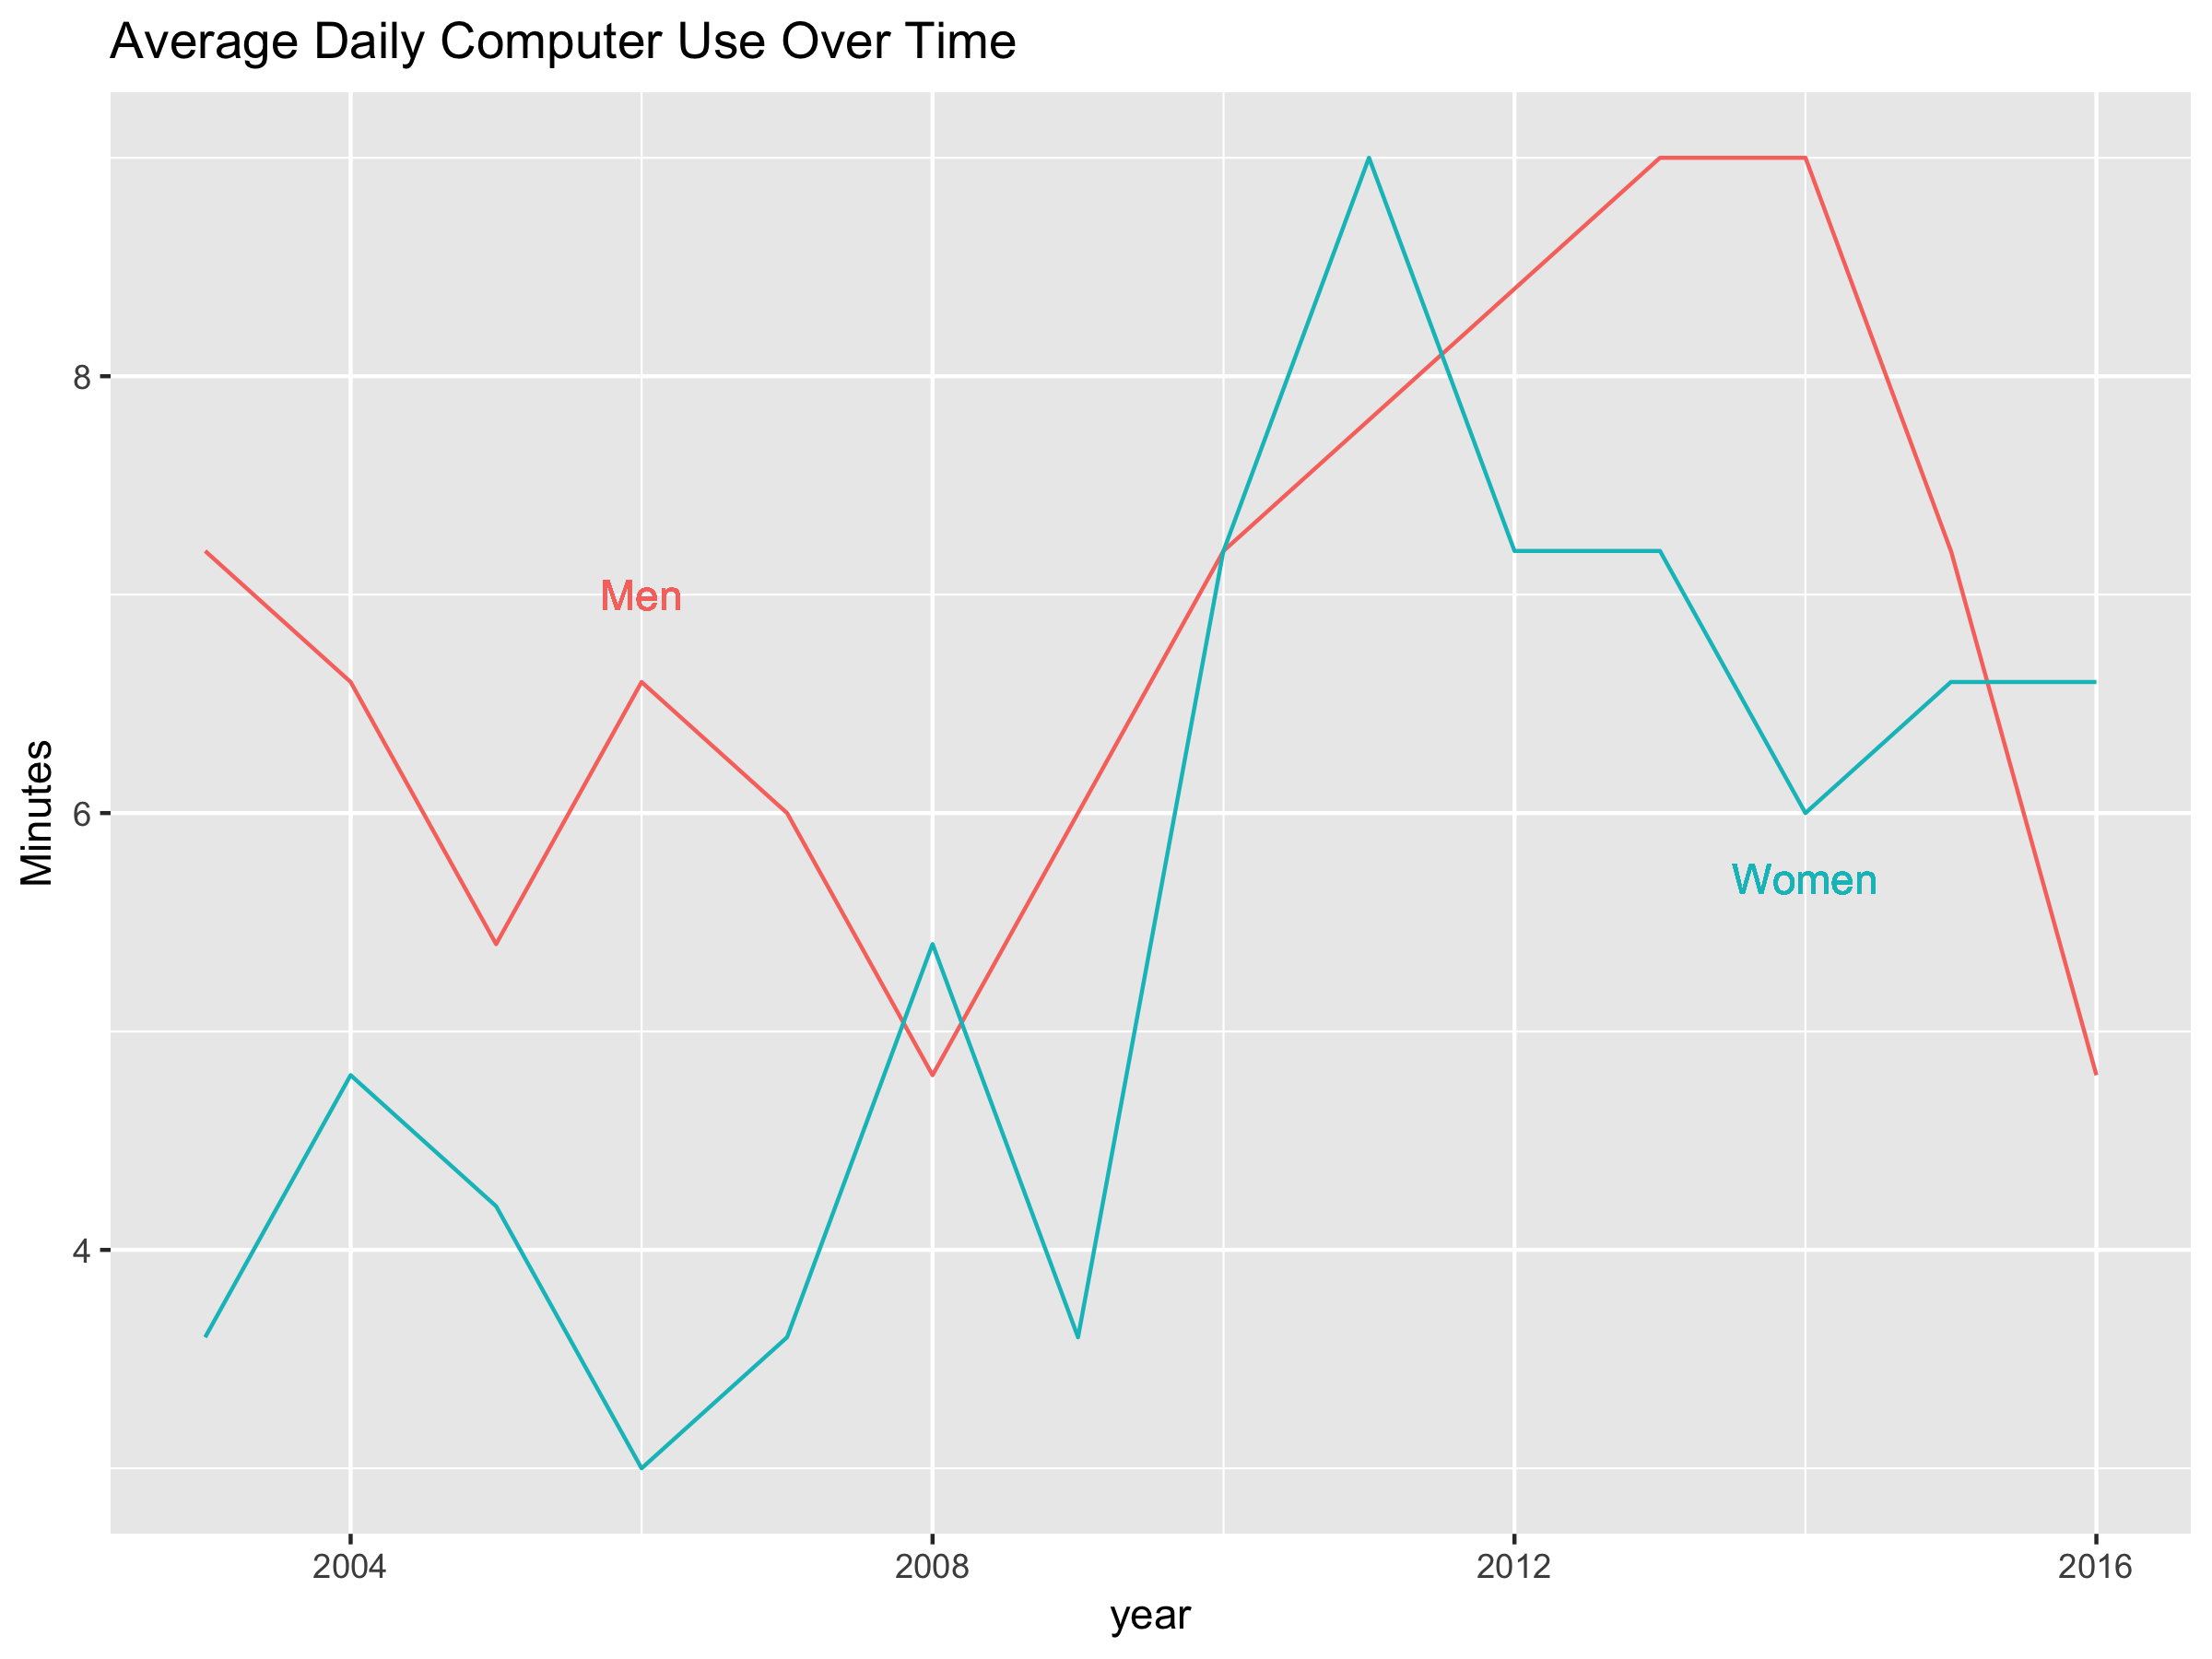
\includegraphics{fig/computer_use_example.png}
\caption{}
\end{figure}

\hypertarget{jitter-rug}{\chapter{Jitter, Rug, and
Aesthetics}\label{jitter-rug}}

\section{Data}\label{data-6}

The \href{https://psidonline.isr.umich.edu}{Panel Study of Income
Dynamics (PSID)} is the longest running longitudinal household survey in
the world.

From the \href{https://simba.isr.umich.edu/data/data.aspx}{Data page},
you can use the \texttt{Data\ Center} to create customized datasets.
We'll use the
\href{https://simba.isr.umich.edu/data/PackagedData.aspx}{Packaged Data}
option. Click the
\href{https://simba.isr.umich.edu/Zips/ZipMain.aspx}{Main and
Supplemental Studies} link. Under the
\texttt{Supplemental\ Studies\ \textgreater{}\ Transition\ into\ Adulthood\ Supplement}
section, select the download for \texttt{2015}.

To download the supplement you will need to sign in or register for a
new account (by clicking the ``New User?'' link). Once you have logged
in you should be able to download the zip file:

\begin{itemize}
\tightlist
\item
  ta2015.zip
\end{itemize}

\subsection{Codebook}\label{codebook}

The \texttt{TA2015\_codebook.pdf} is the perfect place for us to
identify some key variables of interest. The following is an excerpt
listing the variables we will use:

\begin{verbatim}
TA150003  "2015 PSID FAMILY IW (ID) NUMBER"
2015 PSID Family Interview Number

TA150004  "2015 INDIVIDUAL SEQUENCE NUMBER"
2015 PSID Sequence Number
This variable provides a means of identifying an individual's status with regard to the
PSID family unit at the time of the 2015 PSID interview.

Value/Range   Code Value/Range Text
1 - 20        Individuals in the family at the time of the 2015 PSID
              interview
51 - 59       Individuals in institutions at the time of the 2015 PSID
              interview

TA150005 "CURRENT STATE"
Current State (FIPS state codes)

TA150015 "A1_1 HOW SATISFIED W/ LIFE AS A WHOLE"
A1_1. We'd like to start by asking you about life in general. Please think about your
life-as-a-whole. How satisfied are you with it? Are you completely satisfied, very
satisfied, somewhat satisfied, not very satisfied, or not at all satisfied?

Value/Range   Code Value/Range Text
1             Completely satisfied
2             Very satisfied
3             Somewhat satisfied
4             Not very satisfied
5             Not at all satisfied
8             DK

TA150092 "D28A NUMBER OF CHILDREN"
D28a. How many (biological,) adopted, or step-children do you have?

TA150128 "E1 EMPLOYMENT STATUS 1ST MENTION"
E1. Now we have some questions about employment. We would like to know about what you do -
- are you working now, looking for work, keeping house, a student, or what?--1ST MENTION

Value/Range   Code Value/Range Text
1             Working now, including military
2             Only temporarily laid off; sick or maternity leave
3             Looking for work, unemployed
5             Disabled, permanently or temporarily
6             Keeping house
7             Student

TA150512 "F1 HOW MUCH EARN LAST YEAR"
F1. We try to understand how people all over the country are getting along financially, so
now I have some questions about earnings and income. How much did you earn altogether
from work in 2014, that is, before anything was deducted for taxes or other things,
including any income from bonuses, overtime, tips, commissions, military pay or any other
source?

Value/Range     Code Value/Range Text
0 - 5,000,000   Actual amount
    9,999,998   DK
    9,999,999   NA; refused
\end{verbatim}

\subsubsection{FIPS}\label{fips}

In preparation for working with these variables, we can setup arrays to
take the place of the codebook. The \texttt{tigris} package will give us
the FIPS codes for each state:

\begin{verbatim}
install.packages(tigris)
\end{verbatim}

\begin{Shaded}
\begin{Highlighting}[]
\KeywordTok{library}\NormalTok{(tidyverse)}

\NormalTok{state_fips <-}\StringTok{ }\NormalTok{tigris::fips_codes %>%}
\StringTok{  }\KeywordTok{group_by}\NormalTok{(state) %>%}
\StringTok{  }\KeywordTok{summarize}\NormalTok{(}\DataTypeTok{fips =} \KeywordTok{as.numeric}\NormalTok{(}\KeywordTok{first}\NormalTok{(state_code)))}
\NormalTok{fips2state <-}\StringTok{ }\KeywordTok{array}\NormalTok{()}
\NormalTok{fips2state[state_fips$fips] <-}\StringTok{ }\NormalTok{state_fips$state}
\NormalTok{fips2state}
\end{Highlighting}
\end{Shaded}

\begin{verbatim}
##  [1] "AL" "AK" NA   "AZ" "AR" "CA" NA   "CO" "CT" "DE" "DC" "FL" "GA" NA  
## [15] "HI" "ID" "IL" "IN" "IA" "KS" "KY" "LA" "ME" "MD" "MA" "MI" "MN" "MS"
## [29] "MO" "MT" "NE" "NV" "NH" "NJ" "NM" "NY" "NC" "ND" "OH" "OK" "OR" "PA"
## [43] NA   "RI" "SC" "SD" "TN" "TX" "UT" "VT" "VA" NA   "WA" "WV" "WI" "WY"
## [57] NA   NA   NA   "AS" NA   NA   NA   NA   NA   "GU" NA   NA   "MP" NA  
## [71] NA   "PR" NA   "UM" NA   NA   NA   "VI"
\end{verbatim}

\subsubsection{Satisfaction}\label{satisfaction}

\begin{Shaded}
\begin{Highlighting}[]
\NormalTok{satisfaction <-}\StringTok{ }\KeywordTok{array}\NormalTok{()}
\NormalTok{satisfaction_levels <-}\StringTok{ }\KeywordTok{c}\NormalTok{(}\StringTok{"Completely satisfied"}\NormalTok{, }\StringTok{"Very satisfied"}\NormalTok{, }\StringTok{"Somewhat satisfied"}\NormalTok{, }\StringTok{"Not very satisfied"}\NormalTok{, }\StringTok{"Not at all satisfied"}\NormalTok{, }\StringTok{"DK"}\NormalTok{)}
\NormalTok{satisfaction[}\KeywordTok{c}\NormalTok{(}\DecValTok{1}\NormalTok{, }\DecValTok{2}\NormalTok{, }\DecValTok{3}\NormalTok{, }\DecValTok{4}\NormalTok{, }\DecValTok{5}\NormalTok{, }\DecValTok{8}\NormalTok{)] <-}\StringTok{ }\NormalTok{satisfaction_levels}
\NormalTok{satisfaction}
\end{Highlighting}
\end{Shaded}

\begin{verbatim}
## [1] "Completely satisfied" "Very satisfied"       "Somewhat satisfied"  
## [4] "Not very satisfied"   "Not at all satisfied" NA                    
## [7] NA                     "DK"
\end{verbatim}

\subsubsection{Employment Status}\label{employment-status}

We can also specify the array elements one by one:

\begin{Shaded}
\begin{Highlighting}[]
\NormalTok{employment <-}\StringTok{ }\KeywordTok{array}\NormalTok{()}
\NormalTok{employment[}\DecValTok{1}\NormalTok{] <-}\StringTok{ "Working now, including military"}
\NormalTok{employment[}\DecValTok{2}\NormalTok{] <-}\StringTok{ "Only temporarily laid off; sick or maternity leave"}
\NormalTok{employment[}\DecValTok{3}\NormalTok{] <-}\StringTok{ "Looking for work, unemployed"}
\NormalTok{employment[}\DecValTok{5}\NormalTok{] <-}\StringTok{ "Disabled, permanently or temporarily"}
\NormalTok{employment[}\DecValTok{6}\NormalTok{] <-}\StringTok{ "Keeping house"}
\NormalTok{employment[}\DecValTok{7}\NormalTok{] <-}\StringTok{ "Student"}
\NormalTok{employment}
\end{Highlighting}
\end{Shaded}

\begin{verbatim}
## [1] "Working now, including military"                   
## [2] "Only temporarily laid off; sick or maternity leave"
## [3] "Looking for work, unemployed"                      
## [4] NA                                                  
## [5] "Disabled, permanently or temporarily"              
## [6] "Keeping house"                                     
## [7] "Student"
\end{verbatim}

\subsection{Preprocessing the SPSS
File}\label{preprocessing-the-spss-file}

If you don't have them already, open the zip file and move the
\texttt{TA2015.txt} and \texttt{TA2015.sps} files into the \texttt{data}
folder. For our import to work, We need to find a line that needs to be
removed from the top of the sps file. The line we want to remove should
look like the following line:

\begin{verbatim}
FILE HANDLE PSID / NAME = '[PATH]\TA2015.TXT' LRECL = 2173 .
\end{verbatim}

To find this line we can output the first 20 lines of the
\texttt{TA2015.sps} file:

\begin{Shaded}
\begin{Highlighting}[]
\KeywordTok{readLines}\NormalTok{(}\StringTok{"data/TA2015.sps"}\NormalTok{, }\DataTypeTok{n =} \DecValTok{10}\NormalTok{)}
\end{Highlighting}
\end{Shaded}

\begin{verbatim}
##  [1] ""                                                                          
##  [2] "**************************************************************************"
##  [3] "   Label           : Transition to Adulthood Study 2015"                   
##  [4] "   Rows            : 1641"                                                 
##  [5] "   Columns         : 1304"                                                 
##  [6] "   ASCII File Date : July 5, 2017"                                         
##  [7] "*************************************************************************."
##  [8] ""                                                                          
##  [9] "FILE HANDLE PSID / NAME = '[PATH]\\TA2015.TXT' LRECL = 2173 ."             
## [10] "DATA LIST FILE = PSID FIXED /"
\end{verbatim}

Now we know the line to remove is line number 9, we can write a new file
to be used in the processing step below.

\begin{Shaded}
\begin{Highlighting}[]
\NormalTok{input <-}\StringTok{ }\KeywordTok{file}\NormalTok{(}\StringTok{"data/TA2015.sps"}\NormalTok{)}
\NormalTok{output <-}\StringTok{ }\KeywordTok{file}\NormalTok{(}\StringTok{"data/TA2015_clean.sps"}\NormalTok{)}

\KeywordTok{open}\NormalTok{(input, }\DataTypeTok{type =} \StringTok{"r"}\NormalTok{)}
\KeywordTok{open}\NormalTok{(output, }\DataTypeTok{open =} \StringTok{"w"}\NormalTok{)}

\KeywordTok{writeLines}\NormalTok{(}\KeywordTok{readLines}\NormalTok{(input, }\DataTypeTok{n =} \DecValTok{8}\NormalTok{), output)}
\KeywordTok{invisible}\NormalTok{(}\KeywordTok{readLines}\NormalTok{(input, }\DataTypeTok{n =} \DecValTok{1}\NormalTok{))}
\KeywordTok{writeLines}\NormalTok{(}\KeywordTok{readLines}\NormalTok{(input), output)}

\KeywordTok{close}\NormalTok{(input)}
\KeywordTok{close}\NormalTok{(output)}

\KeywordTok{readLines}\NormalTok{(}\StringTok{"data/TA2015_clean.sps"}\NormalTok{, }\DataTypeTok{n =} \DecValTok{10}\NormalTok{)}
\end{Highlighting}
\end{Shaded}

\begin{verbatim}
##  [1] ""                                                                                           
##  [2] "**************************************************************************"                 
##  [3] "   Label           : Transition to Adulthood Study 2015"                                    
##  [4] "   Rows            : 1641"                                                                  
##  [5] "   Columns         : 1304"                                                                  
##  [6] "   ASCII File Date : July 5, 2017"                                                          
##  [7] "*************************************************************************."                 
##  [8] ""                                                                                           
##  [9] "DATA LIST FILE = PSID FIXED /"                                                              
## [10] "      TA150001        1 - 1         TA150002        2 - 6         TA150003        7 - 11   "
\end{verbatim}

\subsection{Importing with the SPSS file using
memisc}\label{importing-with-the-spss-file-using-memisc}

The \texttt{memisc} package has useful tools for importing SPSS and
Stata files that augment what already exists in \texttt{base}.
Unfortunately, one of its dependencies, \texttt{MASS}, will mask the
select method from \texttt{dplyr}. To avoid this, instead of loading
\texttt{memisc} with \texttt{library(memisc)}, we can prefix all
\texttt{memisc} functions with \texttt{memisc::}.

\begin{verbatim}
install.packages("memisc")
\end{verbatim}

\begin{Shaded}
\begin{Highlighting}[]
\NormalTok{ta_importer <-}\StringTok{ }\NormalTok{memisc::}\KeywordTok{spss.fixed.file}\NormalTok{(}\StringTok{"data/TA2015.txt"}\NormalTok{, }\DataTypeTok{columns.file =} \StringTok{"data/TA2015_clean.sps"}\NormalTok{, }\DataTypeTok{varlab.file =} \StringTok{"data/TA2015_clean.sps"}\NormalTok{, }\DataTypeTok{to.lower =} \OtherTok{FALSE}\NormalTok{)}
\NormalTok{ta_full <-}\StringTok{ }\NormalTok{memisc::}\KeywordTok{as.data.set}\NormalTok{(ta_importer)}
\NormalTok{ta_full}
\end{Highlighting}
\end{Shaded}

\begin{verbatim}
## 
## Data set with 1641 observations and 1304 variables
## 
##    TA150001 TA150002 TA150003 TA150004 TA150005 TA150006 TA150007 ...
##  1        1        1     4893        1       37       55        9 ...
##  2        1        2     2967        1       48       57        9 ...
##  3        1        3     6095        5       37       96        9 ...
##  4        1        4     3738        3        8       98        9 ...
##  5        1        5     6741        3       16      104        9 ...
##  6        1        6     4839        1       28       68        9 ...
##  7        1        7     3828        1       48       67        9 ...
##  8        1        8     5640       51       21       88        9 ...
##  9        1        9     5210       52        6       80        9 ...
## 10        1       10      339        3       18       93        9 ...
## 11        1       11     3192        2       26       66        9 ...
## 12        1       12      561        2       26       91        9 ...
## 13        1       13     2500       51       13      100        9 ...
## 14        1       14     5283        2       39       68        9 ...
## 15        1       15     6679        1       24       62        9 ...
## 16        1       16     3286        2        8       67        9 ...
## 17        1       17     3266        2        6      155        9 ...
## 18        1       18     3720        2       48       61        9 ...
## 19        1       19     3714        2       48       82        9 ...
## 20        1       20     6244        1       48       89        9 ...
## 21        1       21     4199        1       13       80        9 ...
## 22        1       22     3962        2       51       86        9 ...
## 23        1       23     2878        1       41       85        9 ...
## 24        1       24     3835        1       37       85        9 ...
## 25        1       25      487       51       13       91        9 ...
## .. ........ ........ ........ ........ ........ ........ ........ ...
## (25 of 1641 observations shown)
\end{verbatim}

\subsection{Transform Data}\label{transform-data}

Take the arrays we created above to process the file down to the
variables we selected.

\begin{Shaded}
\begin{Highlighting}[]
\NormalTok{ta <-}\StringTok{ }\NormalTok{ta_full %>%}
\StringTok{  }\KeywordTok{as.data.frame}\NormalTok{() %>%}
\StringTok{  }\KeywordTok{as.tbl}\NormalTok{() %>%}
\StringTok{  }\KeywordTok{filter}\NormalTok{(TA150005 >}\StringTok{ }\DecValTok{0}\NormalTok{) %>%}\StringTok{ }\CommentTok{# get rid of the 1 non-US response}
\StringTok{  }\KeywordTok{transmute}\NormalTok{(}
    \DataTypeTok{family_id         =} \NormalTok{TA150003, }
    \DataTypeTok{in_institution    =} \NormalTok{TA150004 >}\StringTok{ }\DecValTok{50}\NormalTok{, }
    \DataTypeTok{state             =} \NormalTok{fips2state[TA150005], }
    \DataTypeTok{life_satisfaction =} \KeywordTok{factor}\NormalTok{(satisfaction[TA150015], }\DataTypeTok{levels =} \NormalTok{satisfaction_levels, }\DataTypeTok{ordered =} \OtherTok{TRUE}\NormalTok{), }
    \DataTypeTok{children          =} \NormalTok{TA150092, }
    \DataTypeTok{employment_status =} \NormalTok{employment[TA150128], }
    \DataTypeTok{annual_earnings   =} \NormalTok{TA150512 %>%}\StringTok{ }\KeywordTok{na_if}\NormalTok{(}\DecValTok{9999999}\NormalTok{) %>%}\StringTok{ }\KeywordTok{na_if}\NormalTok{(}\DecValTok{9999999}\NormalTok{)}
  \NormalTok{)}
\NormalTok{ta}
\end{Highlighting}
\end{Shaded}

\begin{verbatim}
## # A tibble: 1,640 x 7
##    family_id in_institution state    life_satisfaction children
##        <dbl>          <lgl> <chr>                <ord>    <dbl>
##  1      4893          FALSE    NC   Somewhat satisfied        0
##  2      2967          FALSE    TX   Somewhat satisfied        0
##  3      6095          FALSE    NC   Somewhat satisfied        0
##  4      3738          FALSE    CO   Somewhat satisfied        0
##  5      6741          FALSE    ID       Very satisfied        0
##  6      4839          FALSE    MS Completely satisfied        1
##  7      3828          FALSE    TX   Somewhat satisfied        0
##  8      5640           TRUE    KY Completely satisfied        0
##  9      5210           TRUE    CA       Very satisfied        0
## 10       339          FALSE    IN   Somewhat satisfied        0
## # ... with 1,630 more rows, and 2 more variables: employment_status <chr>,
## #   annual_earnings <dbl>
\end{verbatim}

\begin{Shaded}
\begin{Highlighting}[]
\KeywordTok{library}\NormalTok{(ggplot2)}
\NormalTok{base_plot <-}\StringTok{ }\KeywordTok{ggplot}\NormalTok{(ta, }\KeywordTok{aes}\NormalTok{(life_satisfaction, annual_earnings)) +}\StringTok{ }\KeywordTok{scale_y_log10}\NormalTok{()}
\NormalTok{base_plot +}\StringTok{ }\KeywordTok{geom_point}\NormalTok{()}
\end{Highlighting}
\end{Shaded}

\includegraphics{09-jitter-rug_files/figure-latex/unnamed-chunk-9-1.pdf}

\section{Jitter}\label{jitter}

When many points overlap, using \texttt{geom\_jitter} adjusts the
position of each point to minimize overlap.

\begin{Shaded}
\begin{Highlighting}[]
\NormalTok{base_plot +}\StringTok{ }\KeywordTok{geom_jitter}\NormalTok{()}
\end{Highlighting}
\end{Shaded}

\includegraphics{09-jitter-rug_files/figure-latex/unnamed-chunk-10-1.pdf}

See how this compares to using \texttt{alpha} (i.e., opacity) to see how
many points are in a given position:

\begin{Shaded}
\begin{Highlighting}[]
\NormalTok{base_plot +}\StringTok{ }\KeywordTok{geom_point}\NormalTok{(}\DataTypeTok{alpha =} \FloatTok{0.1}\NormalTok{)}
\end{Highlighting}
\end{Shaded}

\includegraphics{09-jitter-rug_files/figure-latex/unnamed-chunk-11-1.pdf}

\section{Rug}\label{rug}

Often when there are many points, we want to plot a summary that
presents the general shape of the data.

\begin{Shaded}
\begin{Highlighting}[]
\NormalTok{base_plot +}\StringTok{ }\KeywordTok{geom_violin}\NormalTok{()}
\end{Highlighting}
\end{Shaded}

\includegraphics{09-jitter-rug_files/figure-latex/unnamed-chunk-12-1.pdf}

The \texttt{geom\_rug} gives us a rug plot that we can use to highlight
where actual observations occured when we create these summary plots.

\begin{Shaded}
\begin{Highlighting}[]
\NormalTok{base_plot +}\StringTok{ }\KeywordTok{geom_violin}\NormalTok{() +}\StringTok{ }\KeywordTok{geom_rug}\NormalTok{()}
\end{Highlighting}
\end{Shaded}

\includegraphics{09-jitter-rug_files/figure-latex/unnamed-chunk-13-1.pdf}

Both \texttt{alpha} and \texttt{jitter} can be applied to the rug as
well.

\begin{Shaded}
\begin{Highlighting}[]
\NormalTok{base_plot +}\StringTok{ }\KeywordTok{geom_violin}\NormalTok{() +}\StringTok{ }\KeywordTok{geom_rug}\NormalTok{(}\DataTypeTok{alpha =} \FloatTok{0.1}\NormalTok{, }\DataTypeTok{position =} \StringTok{"jitter"}\NormalTok{)}
\end{Highlighting}
\end{Shaded}

\includegraphics{09-jitter-rug_files/figure-latex/unnamed-chunk-14-1.pdf}

Now we can see that rug did in fact create a line on the x-axis for each
observation. We can use the \texttt{sides} property to only display the
rug on the left and right (\texttt{"lr"})

\begin{Shaded}
\begin{Highlighting}[]
\NormalTok{base_plot +}\StringTok{ }\KeywordTok{geom_violin}\NormalTok{() +}\StringTok{ }\KeywordTok{geom_rug}\NormalTok{(}\DataTypeTok{alpha =} \FloatTok{0.1}\NormalTok{, }\DataTypeTok{position =} \StringTok{"jitter"}\NormalTok{, }\DataTypeTok{sides =} \StringTok{"lr"}\NormalTok{)}
\end{Highlighting}
\end{Shaded}

\includegraphics{09-jitter-rug_files/figure-latex/unnamed-chunk-15-1.pdf}

\section{Aesthetics}\label{aesthetics}

Aesthetics are the visual properties that define each graph. In ggplot,
the \texttt{aes()} function is used to create a mapping from your data
to these visual properties. We most often use \texttt{aes()} to map our
variables to the \texttt{x} and \texttt{y} dimension. Above, we used the
fact that the first two arguments to \texttt{aes()} are \texttt{x} and
\texttt{y}. That is,

\begin{verbatim}
aes(x = life_satisfaction, y = annual_earnings)
\end{verbatim}

gives the same result as

\begin{verbatim}
aes(life_satisfaction, annual_earnings)
\end{verbatim}

Anytime we want more than two dimensions of our data displayed, it's
useful to map the extra variables to other features of our graph (e.g.,
size, color, alpha, etc.). Let's add number of children to our graph
assigning children to color. (In ggplot both American and British
spellings are supported, so you can use \texttt{color} or
\texttt{colour}.)

\begin{Shaded}
\begin{Highlighting}[]
\KeywordTok{ggplot}\NormalTok{(ta, }\KeywordTok{aes}\NormalTok{(life_satisfaction, annual_earnings, }\DataTypeTok{color =} \NormalTok{children)) +}\StringTok{ }
\StringTok{  }\KeywordTok{scale_y_log10}\NormalTok{() +}\StringTok{ }
\StringTok{  }\KeywordTok{geom_jitter}\NormalTok{()}
\end{Highlighting}
\end{Shaded}

\includegraphics{09-jitter-rug_files/figure-latex/unnamed-chunk-16-1.pdf}

If the \texttt{children} variable was a factor, more distinct colors
would have been chosen. We can see this by coloring by
\texttt{employment\_status} instead.

\begin{Shaded}
\begin{Highlighting}[]
\KeywordTok{ggplot}\NormalTok{(ta, }\KeywordTok{aes}\NormalTok{(life_satisfaction, annual_earnings, }\DataTypeTok{color =} \NormalTok{employment_status)) +}\StringTok{ }
\StringTok{  }\KeywordTok{scale_y_log10}\NormalTok{() +}\StringTok{ }
\StringTok{  }\KeywordTok{geom_jitter}\NormalTok{()}
\end{Highlighting}
\end{Shaded}

\includegraphics{09-jitter-rug_files/figure-latex/unnamed-chunk-17-1.pdf}

You can emphasize a variable by encoding in more than one visual
aesthetic. Let's map \texttt{children} to \texttt{color}, \texttt{size},
and \texttt{alpha}.

\begin{Shaded}
\begin{Highlighting}[]
\KeywordTok{ggplot}\NormalTok{(ta, }\KeywordTok{aes}\NormalTok{(life_satisfaction, annual_earnings, }\DataTypeTok{color =} \NormalTok{children, }\DataTypeTok{size =} \NormalTok{children, }\DataTypeTok{alpha =} \NormalTok{children)) +}\StringTok{ }
\StringTok{  }\KeywordTok{scale_y_log10}\NormalTok{(}\StringTok{"Annual Earnings"}\NormalTok{, }\DataTypeTok{labels =} \NormalTok{scales::dollar) +}\StringTok{ }
\StringTok{  }\KeywordTok{geom_jitter}\NormalTok{()}
\end{Highlighting}
\end{Shaded}

\includegraphics{09-jitter-rug_files/figure-latex/unnamed-chunk-18-1.pdf}

\section{Assignment}\label{assignment-8}

Open the codebook (\texttt{data/TA2015\_codebook.pdf}) and search for
two new variables to visualize. Create a plot that makes use of both
jitter and rug.

\hypertarget{themes-labels-colors}{\chapter{Themes, Labels, and
Colors}\label{themes-labels-colors}}

This lecture uses the following packages:

\begin{verbatim}
tidyverse
lubridate
ggthemes
grid
gridExtra
\end{verbatim}

\section{Data}\label{data-7}

\subsection{Zillow Real Estate Data}\label{zillow-real-estate-data}

\href{https://www.zillow.com/}{Zillow} is an online marketplace for real
estate. It facilitates connection between buyers and sellers, and in the
process collects a large amount of useful economic statistics.

From
\href{https://www.zillow.com/research/data/\#other-metrics}{Zillow's
research data page}, we will download the
\href{http://files.zillowstatic.com/research/public/Metro/AgeOfInventory_Metro_Public.csv}{Age
of Inventory (Days)} CSV. Their list of data definitions at the bottom
of the page includes the following entry:

\emph{Age of Inventory}: Each Wednesday, age of inventory is calculated
as the median number of days all active listings as of that Wednesday
have been current. These medians are then aggregated into the number
reported by taking the median across weekly values.

\begin{Shaded}
\begin{Highlighting}[]
\KeywordTok{library}\NormalTok{(readr)}
\NormalTok{raw_inventory <-}\StringTok{ }\KeywordTok{read_csv}\NormalTok{(}\StringTok{"data/AgeOfInventory_Metro_Public.csv"}\NormalTok{)}
\KeywordTok{head}\NormalTok{(raw_inventory)[,}\DecValTok{1}\NormalTok{:}\DecValTok{6}\NormalTok{]}
\end{Highlighting}
\end{Shaded}

\begin{verbatim}
## # A tibble: 6 x 6
##              RegionName RegionType StateFullName DataTypeDescription
##                   <chr>      <chr>         <chr>               <chr>
## 1         United States    Country          <NA>           All Homes
## 2          New York, NY        Msa      New York           All Homes
## 3           Chicago, IL        Msa      Illinois           All Homes
## 4 Dallas-Fort Worth, TX        Msa         Texas           All Homes
## 5      Philadelphia, PA        Msa  Pennsylvania           All Homes
## 6           Houston, TX        Msa         Texas           All Homes
## # ... with 2 more variables: `2012-01` <int>, `2012-02` <int>
\end{verbatim}

\subsection{\texorpdfstring{Reshaping data with
\texttt{tidyr}}{Reshaping data with tidyr}}\label{reshaping-data-with-tidyr}

Since this data set uses a separate column for each time period, the
data is not yet
\href{https://cran.r-project.org/web/packages/tidyr/vignettes/tidy-data.html}{tidy}.
Let's fix that. We'll use the \texttt{gather()} function from the
\texttt{tidyr} package
(\url{http://tidyr.tidyverse.org/reference/gather.html}) to identify the
name for the new column that stores the old column names
(\texttt{month}), the name for the new column that stores the values in
the columns being reshaped (\texttt{age}), and a column selector to
identify which columns to reshape (\texttt{matches()} takes a regular
expression, see the \texttt{regex} documentation). Lastly, we need to
\texttt{mutate()} the \texttt{month} using \texttt{ymd()} from the
\texttt{lubridate} package. Into \texttt{ymd()}, we place the original
date character (in ``YYYY-MM'' format) and add a piece for the day
(using the ``-DD'' format), so that each of our month time markers are
interpreted as the first day of the corresponding month.

\begin{Shaded}
\begin{Highlighting}[]
\KeywordTok{library}\NormalTok{(lubridate)}
\NormalTok{if(}\StringTok{"package:dplyr"} \NormalTok\StringTok{ }\KeywordTok{search}\NormalTok{()) }\KeywordTok{detach}\NormalTok{(}\StringTok{"package:dplyr"}\NormalTok{, }\DataTypeTok{unload=}\OtherTok{TRUE}\NormalTok{)}
\KeywordTok{library}\NormalTok{(dplyr)}
\KeywordTok{library}\NormalTok{(tidyr)}
\NormalTok{inventory <-}\StringTok{ }\NormalTok{raw_inventory %>%}\StringTok{ }\KeywordTok{select}\NormalTok{(RegionName, }\KeywordTok{matches}\NormalTok{(}\StringTok{"[[:digit:]]"}\NormalTok{)) %>%}
\StringTok{  }\KeywordTok{gather}\NormalTok{(month, age, }\KeywordTok{matches}\NormalTok{(}\StringTok{"[[:digit:]]"}\NormalTok{)) %>%}\StringTok{ }
\StringTok{  }\KeywordTok{mutate}\NormalTok{(}\DataTypeTok{month =} \KeywordTok{ymd}\NormalTok{(}\KeywordTok{paste0}\NormalTok{(month, }\StringTok{"-01"}\NormalTok{)))}
\NormalTok{inventory}
\end{Highlighting}
\end{Shaded}

\begin{verbatim}
## # A tibble: 22,713 x 3
##                   RegionName      month   age
##                        <chr>     <date> <int>
##  1             United States 2012-01-01   120
##  2              New York, NY 2012-01-01   136
##  3               Chicago, IL 2012-01-01   141
##  4     Dallas-Fort Worth, TX 2012-01-01   109
##  5          Philadelphia, PA 2012-01-01   132
##  6               Houston, TX 2012-01-01   112
##  7            Washington, DC 2012-01-01   105
##  8 Miami-Fort Lauderdale, FL 2012-01-01    89
##  9               Atlanta, GA 2012-01-01    98
## 10                Boston, MA 2012-01-01   116
## # ... with 22,703 more rows
\end{verbatim}

\section{Starting Plot}\label{starting-plot}

Let's start with a simple line plot of all these series. Let's show what
happens if we leave out the group and color aesthetic.

\begin{Shaded}
\begin{Highlighting}[]
\KeywordTok{library}\NormalTok{(ggplot2)}
\NormalTok{inventory %>%}\StringTok{ }\KeywordTok{ggplot}\NormalTok{(}\KeywordTok{aes}\NormalTok{(month, age)) +}\StringTok{ }\KeywordTok{geom_line}\NormalTok{()}
\end{Highlighting}
\end{Shaded}

\includegraphics{10-themes-labels-colors_files/figure-latex/unnamed-chunk-4-1.pdf}

Now, let's add in the \texttt{group} \texttt{aes}.

\begin{Shaded}
\begin{Highlighting}[]
\NormalTok{inventory %>%}\StringTok{ }\KeywordTok{ggplot}\NormalTok{(}\KeywordTok{aes}\NormalTok{(month, age, }\DataTypeTok{group =} \NormalTok{RegionName)) +}\StringTok{ }\KeywordTok{geom_line}\NormalTok{()}
\end{Highlighting}
\end{Shaded}

\includegraphics{10-themes-labels-colors_files/figure-latex/unnamed-chunk-5-1.pdf}

It's hard to see what is happening in this tangled mess. Setting
\texttt{alpha} to 0.1 will make this easier to untangle.

\begin{Shaded}
\begin{Highlighting}[]
\NormalTok{basic_plot <-}\StringTok{ }\NormalTok{inventory %>%}\StringTok{ }\KeywordTok{ggplot}\NormalTok{(}\KeywordTok{aes}\NormalTok{(month, age, }\DataTypeTok{group =} \NormalTok{RegionName)) +}\StringTok{ }\KeywordTok{geom_line}\NormalTok{(}\DataTypeTok{alpha =} \FloatTok{0.1}\NormalTok{)}
\NormalTok{basic_plot}
\end{Highlighting}
\end{Shaded}

\includegraphics{10-themes-labels-colors_files/figure-latex/unnamed-chunk-6-1.pdf}

Let's emphasize the line for Honolulu.

\begin{Shaded}
\begin{Highlighting}[]
\NormalTok{basic_plot +}
\StringTok{  }\KeywordTok{geom_line}\NormalTok{(}\DataTypeTok{data =} \NormalTok{inventory %>%}\StringTok{ }\KeywordTok{filter}\NormalTok{(}\KeywordTok{grepl}\NormalTok{(}\StringTok{"Honolulu"}\NormalTok{, RegionName)), }\KeywordTok{aes}\NormalTok{(month, age), }\DataTypeTok{color =} \StringTok{"blue"}\NormalTok{)}
\end{Highlighting}
\end{Shaded}

\includegraphics{10-themes-labels-colors_files/figure-latex/unnamed-chunk-7-1.pdf}

\section{Themes}\label{themes}

\subsection{Complete Themes}\label{complete-themes}

There are a variety of pre-made themes that can make our figures look
cleaner (\url{http://ggplot2.tidyverse.org/reference/ggtheme.html}).
\texttt{theme\_bw()} is good if you don't want to print all the grey
from the default, but you still want the same basic structure.

\begin{Shaded}
\begin{Highlighting}[]
\NormalTok{basic_plot +}\StringTok{ }\KeywordTok{theme_bw}\NormalTok{()}
\end{Highlighting}
\end{Shaded}

\includegraphics{10-themes-labels-colors_files/figure-latex/unnamed-chunk-8-1.pdf}

\texttt{theme\_minimal()} removes some of the visual clutter, removing
the plot border and the axis ticks.

\begin{Shaded}
\begin{Highlighting}[]
\NormalTok{basic_plot +}\StringTok{ }\KeywordTok{theme_minimal}\NormalTok{()}
\end{Highlighting}
\end{Shaded}

\includegraphics{10-themes-labels-colors_files/figure-latex/unnamed-chunk-9-1.pdf}

\texttt{theme\_void()} goes the whole way and removes everything, but
the data. It even removes the axis labels.

\begin{Shaded}
\begin{Highlighting}[]
\NormalTok{basic_plot +}\StringTok{ }\KeywordTok{theme_void}\NormalTok{()}
\end{Highlighting}
\end{Shaded}

\includegraphics{10-themes-labels-colors_files/figure-latex/unnamed-chunk-10-1.pdf}

\subsection{Modifying a theme}\label{modifying-a-theme}

To modify a theme, we just add a call to the \texttt{theme()} function
and assign new values to the parts of the plot we want to change (see
the \texttt{theme()} reference for more examples:
\url{http://ggplot2.tidyverse.org/reference/theme.html}).

Let's start with the \texttt{theme\_bw()} and make the chart more
minimal.

\begin{Shaded}
\begin{Highlighting}[]
\NormalTok{basic_plot +}\StringTok{ }\KeywordTok{theme_bw}\NormalTok{() +}\StringTok{ }\KeywordTok{theme}\NormalTok{(}
  \DataTypeTok{panel.border =} \KeywordTok{element_blank}\NormalTok{(),}
  \DataTypeTok{panel.grid =} \KeywordTok{element_blank}\NormalTok{(),}
  \DataTypeTok{axis.line =} \KeywordTok{element_line}\NormalTok{(}\DataTypeTok{color =} \StringTok{"grey"}\NormalTok{),}
  \DataTypeTok{axis.ticks =} \KeywordTok{element_line}\NormalTok{(}\DataTypeTok{color =} \StringTok{"grey"}\NormalTok{),}
  \DataTypeTok{axis.title.y =} \KeywordTok{element_text}\NormalTok{(}\DataTypeTok{angle =} \DecValTok{0}\NormalTok{)}
\NormalTok{)}
\end{Highlighting}
\end{Shaded}

\includegraphics{10-themes-labels-colors_files/figure-latex/unnamed-chunk-11-1.pdf}

\subsection{\texorpdfstring{\texttt{ggthemes}}{ggthemes}}\label{ggthemes}

The \texttt{ggthemes} package adds a large set of fun themes. See the
vignette at
\url{https://cran.r-project.org/web/packages/ggthemes/vignettes/ggthemes.html}
or enter the following command locally after installing the package

\begin{verbatim}
install.packages("ggthemes")
vignette("ggthemes", package = "ggthemes")
\end{verbatim}

To make our chart look like it came out of the economist, let's use
\texttt{theme\_economist()}. To make the line colors work, we'll use the
\texttt{economist\_pal()} color pal

\begin{Shaded}
\begin{Highlighting}[]
\KeywordTok{library}\NormalTok{(ggthemes)}
\NormalTok{theme_colors <-}\StringTok{ }\KeywordTok{economist_pal}\NormalTok{()(}\DecValTok{2}\NormalTok{)}
\NormalTok{inventory %>%}\StringTok{ }\KeywordTok{ggplot}\NormalTok{(}\KeywordTok{aes}\NormalTok{(month, age, }\DataTypeTok{group =} \NormalTok{RegionName)) +}\StringTok{ }
\StringTok{  }\KeywordTok{geom_line}\NormalTok{(}\DataTypeTok{color =} \NormalTok{theme_colors[}\DecValTok{1}\NormalTok{], }\DataTypeTok{alpha =} \FloatTok{0.1}\NormalTok{) +}
\StringTok{  }\KeywordTok{geom_line}\NormalTok{(}\DataTypeTok{data =} \NormalTok{inventory %>%}\StringTok{ }\KeywordTok{filter}\NormalTok{(}\KeywordTok{grepl}\NormalTok{(}\StringTok{"Honolulu"}\NormalTok{, RegionName)), }
            \KeywordTok{aes}\NormalTok{(month, age), }
            \DataTypeTok{color =} \NormalTok{theme_colors[}\DecValTok{2}\NormalTok{]) +}\StringTok{ }
\StringTok{  }\KeywordTok{theme_economist}\NormalTok{()}
\end{Highlighting}
\end{Shaded}

\includegraphics{10-themes-labels-colors_files/figure-latex/unnamed-chunk-12-1.pdf}

Now let's try out the theme named for \url{http://fivethirtyeight.com/}.

\begin{Shaded}
\begin{Highlighting}[]
\NormalTok{theme_colors <-}\StringTok{ }\KeywordTok{fivethirtyeight_pal}\NormalTok{()(}\DecValTok{2}\NormalTok{)}
\NormalTok{five38 <-}\StringTok{ }\NormalTok{inventory %>%}\StringTok{ }\KeywordTok{ggplot}\NormalTok{(}\KeywordTok{aes}\NormalTok{(month, age, }\DataTypeTok{group =} \NormalTok{RegionName)) +}\StringTok{ }
\StringTok{  }\KeywordTok{geom_line}\NormalTok{(}\DataTypeTok{color =} \NormalTok{theme_colors[}\DecValTok{1}\NormalTok{], }\DataTypeTok{alpha =} \FloatTok{0.1}\NormalTok{) +}
\StringTok{  }\KeywordTok{geom_line}\NormalTok{(}\DataTypeTok{data =} \NormalTok{inventory %>%}\StringTok{ }\KeywordTok{filter}\NormalTok{(}\KeywordTok{grepl}\NormalTok{(}\StringTok{"Honolulu"}\NormalTok{, RegionName)), }
            \KeywordTok{aes}\NormalTok{(month, age), }
            \DataTypeTok{color =} \NormalTok{theme_colors[}\DecValTok{2}\NormalTok{]) +}\StringTok{ }
\StringTok{  }\KeywordTok{theme_fivethirtyeight}\NormalTok{()}
\NormalTok{five38}
\end{Highlighting}
\end{Shaded}

\includegraphics{10-themes-labels-colors_files/figure-latex/unnamed-chunk-13-1.pdf}

\section{Labels}\label{labels}

Now that we have a nice looking basic chart, we need to make sure our
labels are in the right places and give enough information.

\subsection{Title}\label{title}

Let's start by adding a title. For a time series like this, using the
name of the variable on the x-axis is a good start. We can also change
the x-axis to break at each year, which makes the seasonality of this
series even easier to pick out. With these added vertical lines, our
chart will be more readable if we remove the horizontal gridlines
(\texttt{panel.grid.major.y}).

\begin{Shaded}
\begin{Highlighting}[]
\NormalTok{five38_with_title <-}\StringTok{ }\NormalTok{five38 +}\StringTok{ }
\StringTok{  }\KeywordTok{ggtitle}\NormalTok{(}\StringTok{"Median Days Listed by Metro Area"}\NormalTok{) +}\StringTok{ }
\StringTok{  }\KeywordTok{scale_x_date}\NormalTok{(}\DataTypeTok{date_breaks =} \StringTok{"1 year"}\NormalTok{, }\DataTypeTok{date_labels =} \StringTok{"%Y"}\NormalTok{) +}
\StringTok{  }\KeywordTok{theme}\NormalTok{(}\DataTypeTok{panel.grid.major.y =} \KeywordTok{element_blank}\NormalTok{())}
\NormalTok{five38_with_title}
\end{Highlighting}
\end{Shaded}

\includegraphics{10-themes-labels-colors_files/figure-latex/unnamed-chunk-14-1.pdf}

Since we used our title wisely we don't need to add a y-axis title. The
x-axis is time and this is fairly obvious, so we can also leave off the
x-axis title. What we should do is label the highlighted series.

\begin{Shaded}
\begin{Highlighting}[]
\NormalTok{last_hnl <-}\StringTok{ }\NormalTok{inventory %>%}
\StringTok{  }\KeywordTok{filter}\NormalTok{(}\KeywordTok{grepl}\NormalTok{(}\StringTok{"Honolulu"}\NormalTok{, RegionName)) %>%}
\StringTok{  }\KeywordTok{top_n}\NormalTok{(}\DecValTok{1}\NormalTok{, month)}
\NormalTok{gg <-}\StringTok{ }\NormalTok{five38_with_title +}\StringTok{ }
\StringTok{  }\KeywordTok{geom_text}\NormalTok{(}\DataTypeTok{data =} \NormalTok{last_hnl, }\DataTypeTok{label =} \NormalTok{last_hnl$RegionName,}
            \DataTypeTok{hjust =} \StringTok{"left"}\NormalTok{, }\DataTypeTok{nudge_x =} \DecValTok{70}\NormalTok{)}
\NormalTok{gg}
\end{Highlighting}
\end{Shaded}

\includegraphics{10-themes-labels-colors_files/figure-latex/unnamed-chunk-15-1.pdf}

To adjust the margins, we have to drill deeper than ggplot. I found the
following approach through searching for \texttt{ggplot\ clipping}
(\url{https://rud.is/b/2015/08/27/coloring-and-drawing-outside-the-lines-in-ggplot/}).

\begin{Shaded}
\begin{Highlighting}[]
\KeywordTok{library}\NormalTok{(gridExtra)}
\KeywordTok{library}\NormalTok{(grid)}
\NormalTok{gb <-}\StringTok{ }\KeywordTok{ggplot_build}\NormalTok{(gg +}\StringTok{ }\KeywordTok{theme}\NormalTok{(}\DataTypeTok{plot.margin =} \KeywordTok{unit}\NormalTok{(}\KeywordTok{c}\NormalTok{(}\DecValTok{1}\NormalTok{, }\DecValTok{7}\NormalTok{, }\DecValTok{2}\NormalTok{, }\DecValTok{1}\NormalTok{), }\StringTok{"lines"}\NormalTok{)))}
\NormalTok{gt <-}\StringTok{ }\KeywordTok{ggplot_gtable}\NormalTok{(gb)}

\NormalTok{gt$layout$clip[gt$layout$name==}\StringTok{"panel"}\NormalTok{] <-}\StringTok{ "off"}

\KeywordTok{grid.draw}\NormalTok{(gt)}
\end{Highlighting}
\end{Shaded}

\includegraphics{10-themes-labels-colors_files/figure-latex/unnamed-chunk-16-1.pdf}

\section{Colors}\label{colors}

Color is an important tool in creating engaging and informative
visualizations. Color is often used to encode a dimension not already
displayed in a chart (e.g., adding a third dimension to a scatter plot).
Above, we used color to highlight a specific set of data points. We used
a highlight color for Urban Honolulu and set the other metro areas to a
blue with transparency.

\subsection{Color Scales}\label{color-scales}

An easy way to see the colors within a given color scheme is by using
the \texttt{show\_col()} function in the \texttt{scales} package. We can
use it to show the colors in the \texttt{theme\_colors} variable we
created above.

\begin{Shaded}
\begin{Highlighting}[]
\KeywordTok{library}\NormalTok{(scales)}
\KeywordTok{show_col}\NormalTok{(theme_colors)}
\end{Highlighting}
\end{Shaded}

\includegraphics{10-themes-labels-colors_files/figure-latex/unnamed-chunk-17-1.pdf}

The combinations of letters and numbers in the color squares is the hex
representation of the red, green, and blue color values that make up the
given color (e.g., \texttt{\#008FD5}). Adobe has a fun color chooser
where you can paste these hex values and create your own color scheme:

\url{https://color.adobe.com/}

There are not many colors in the \texttt{fivethirtyeight\_pal()} color
palette (only 3). The \texttt{economist\_pal()} palette has 11, which is
a bit better for categorical data:

\begin{Shaded}
\begin{Highlighting}[]
\KeywordTok{show_col}\NormalTok{(}\KeywordTok{economist_pal}\NormalTok{()(}\DecValTok{11}\NormalTok{))}
\end{Highlighting}
\end{Shaded}

\includegraphics{10-themes-labels-colors_files/figure-latex/unnamed-chunk-18-1.pdf}

\subsection{Color Brewer}\label{color-brewer}

Color Brewer (\url{http://colorbrewer2.org/}) is the gold standard for
color choice in maps. The online tool allows you to preview and export
color schemes that are designed for accessibility (i.e., color-blind
safe) and for the main strategies for encoding data using color
(sequential, diverging, and qualitative). Most of these scales are
available within ggplot
(\url{http://ggplot2.tidyverse.org/reference/scale_brewer.html}).

\begin{Shaded}
\begin{Highlighting}[]
\NormalTok{RColorBrewer::brewer.pal.info}
\end{Highlighting}
\end{Shaded}

\begin{verbatim}
##          maxcolors category colorblind
## BrBG            11      div       TRUE
## PiYG            11      div       TRUE
## PRGn            11      div       TRUE
## PuOr            11      div       TRUE
## RdBu            11      div       TRUE
## RdGy            11      div      FALSE
## RdYlBu          11      div       TRUE
## RdYlGn          11      div      FALSE
## Spectral        11      div      FALSE
## Accent           8     qual      FALSE
## Dark2            8     qual       TRUE
## Paired          12     qual       TRUE
## Pastel1          9     qual      FALSE
## Pastel2          8     qual      FALSE
## Set1             9     qual      FALSE
## Set2             8     qual       TRUE
## Set3            12     qual      FALSE
## Blues            9      seq       TRUE
## BuGn             9      seq       TRUE
## BuPu             9      seq       TRUE
## GnBu             9      seq       TRUE
## Greens           9      seq       TRUE
## Greys            9      seq       TRUE
## Oranges          9      seq       TRUE
## OrRd             9      seq       TRUE
## PuBu             9      seq       TRUE
## PuBuGn           9      seq       TRUE
## PuRd             9      seq       TRUE
## Purples          9      seq       TRUE
## RdPu             9      seq       TRUE
## Reds             9      seq       TRUE
## YlGn             9      seq       TRUE
## YlGnBu           9      seq       TRUE
## YlOrBr           9      seq       TRUE
## YlOrRd           9      seq       TRUE
\end{verbatim}

\begin{Shaded}
\begin{Highlighting}[]
\KeywordTok{show_col}\NormalTok{(}\KeywordTok{brewer_pal}\NormalTok{(}\DataTypeTok{palette =} \StringTok{"Accent"}\NormalTok{)(}\DecValTok{8}\NormalTok{))}
\end{Highlighting}
\end{Shaded}

\includegraphics{10-themes-labels-colors_files/figure-latex/unnamed-chunk-20-1.pdf}

Here's how to take this color palette and apply it to our previous
chart:

\begin{Shaded}
\begin{Highlighting}[]
\NormalTok{theme_colors <-}\StringTok{ }\KeywordTok{brewer_pal}\NormalTok{(}\DataTypeTok{palette =} \StringTok{"Accent"}\NormalTok{)(}\DecValTok{8}\NormalTok{)}
\NormalTok{inventory %>%}\StringTok{ }\KeywordTok{ggplot}\NormalTok{(}\KeywordTok{aes}\NormalTok{(month, age, }\DataTypeTok{group =} \NormalTok{RegionName)) +}\StringTok{ }
\StringTok{  }\KeywordTok{geom_line}\NormalTok{(}\DataTypeTok{color =} \NormalTok{theme_colors[}\DecValTok{1}\NormalTok{], }\DataTypeTok{alpha =} \FloatTok{0.1}\NormalTok{) +}
\StringTok{  }\KeywordTok{geom_line}\NormalTok{(}\DataTypeTok{data =} \NormalTok{inventory %>%}\StringTok{ }\KeywordTok{filter}\NormalTok{(}\KeywordTok{grepl}\NormalTok{(}\StringTok{"Honolulu"}\NormalTok{, RegionName)), }
            \KeywordTok{aes}\NormalTok{(month, age), }
            \DataTypeTok{color =} \NormalTok{theme_colors[}\DecValTok{2}\NormalTok{]) +}\StringTok{ }
\StringTok{  }\KeywordTok{theme_fivethirtyeight}\NormalTok{()}
\end{Highlighting}
\end{Shaded}

\includegraphics{10-themes-labels-colors_files/figure-latex/unnamed-chunk-21-1.pdf}

\section{Assignment}\label{assignment-9}

Using the same file, pick a different time series to emphasize (with a
different color) and choose a different theme.

\hypertarget{polar}{\chapter{Polar Coordinates}\label{polar}}

This lecture uses the following packages:

\begin{verbatim}
tidyverse
lubridate
forcats
\end{verbatim}

\section{Data}\label{data-8}

\subsection*{Survey of Consumers}\label{survey-of-consumers}
\addcontentsline{toc}{subsection}{Survey of Consumers}

The University of Michigan conducts the Survey of Consumers. This
monthly survey takes the pulse of consumers to help predict the state of
the economy in the near future. We will be using a few responses from
this monthly survey to highlight how you can visualize periodic data.
For full definitions of the variables we will work with take a look at
the online codebook:
\url{https://data.sca.isr.umich.edu/subset/codebook.php}

To download the data

\begin{enumerate}
\def\labelenumi{\arabic{enumi}.}
\tightlist
\item
  Go to the Survey of Consumers' data page:
  \url{https://data.sca.isr.umich.edu/subset/subset.php}
\item
  In the \textbf{Frequency and Range} section, set the \textbf{Starting
  year} to 1998, since that is the first year with complete data on
  ``Probability of Losing a Job During the Next 5 Years'' (PJOB)
\item
  In the \textbf{Demographics} section, check all Income groups (y13 =
  \emph{Bottom 33\%}, y23 = \emph{Middle 33\%}, and y33 = \emph{Top
  33\%})
\item
  In the \textbf{Variables} section, check \emph{PEXP} and \emph{PJOB}
  in the \textbf{Personal Finances} subsection, and check \emph{UMEX} in
  the \textbf{Unemployment, Interest Rates, Prices, Government
  Expectations} subsection
\item
  Click on the ``Download CSV'' button.
\end{enumerate}

Load the downloaded dataset.

\begin{Shaded}
\begin{Highlighting}[]
\KeywordTok{library}\NormalTok{(tidyverse)}
\NormalTok{survey <-}\StringTok{ }\KeywordTok{read_csv}\NormalTok{(}\StringTok{"data/scaum-814.csv"}\NormalTok{)}
\end{Highlighting}
\end{Shaded}

Divide the date column into year and month columns.

\begin{Shaded}
\begin{Highlighting}[]
\KeywordTok{library}\NormalTok{(lubridate)}
\NormalTok{survey <-}\StringTok{ }\NormalTok{survey %>%}
\StringTok{  }\KeywordTok{mutate}\NormalTok{(}\DataTypeTok{date =} \KeywordTok{parse_date}\NormalTok{(yyyymm, }\DataTypeTok{format =} \StringTok{"%Y%m"}\NormalTok{),}
         \DataTypeTok{year =} \KeywordTok{year}\NormalTok{(date),}
         \DataTypeTok{month =} \KeywordTok{month}\NormalTok{(date)}
  \NormalTok{) %>%}
\StringTok{  }\KeywordTok{select}\NormalTok{(-yyyymm)}
\NormalTok{survey}
\end{Highlighting}
\end{Shaded}

\begin{verbatim}
## # A tibble: 235 x 12
##    pexp_r_y13 pexp_r_y23 pexp_r_y33 pjob_mean_y13 pjob_mean_y23
##         <int>      <int>      <int>         <dbl>         <dbl>
##  1        128        153        148          15.3          16.6
##  2        147        143        149          18.9          19.8
##  3        125        141        137          14.4          16.4
##  4        133        134        149          14.2          18.5
##  5        126        129        150          15.8          16.8
##  6        128        139        137          14.4          14.8
##  7        132        142        146          17.0          18.6
##  8        131        143        145          15.8          19.3
##  9        126        135        135          18.1          17.2
## 10        132        134        136          19.4          16.6
## # ... with 225 more rows, and 7 more variables: pjob_mean_y33 <dbl>,
## #   umex_r_y13 <int>, umex_r_y23 <int>, umex_r_y33 <int>, date <date>,
## #   year <dbl>, month <dbl>
\end{verbatim}

Each variable is calculated from the survey as follows:

\begin{longtable}[]{@{}lll@{}}
\toprule
\begin{minipage}[b]{0.09\columnwidth}\raggedright\strut
Code\strut
\end{minipage} & \begin{minipage}[b]{0.28\columnwidth}\raggedright\strut
Survey Question\strut
\end{minipage} & \begin{minipage}[b]{0.20\columnwidth}\raggedright\strut
Calculation\strut
\end{minipage}\tabularnewline
\midrule
\endhead
\begin{minipage}[t]{0.09\columnwidth}\raggedright\strut
PEXP\strut
\end{minipage} & \begin{minipage}[t]{0.28\columnwidth}\raggedright\strut
``Now looking ahead -- do you think that a year from now you (and your
family living there) will be better off financially, worse off, or just
about the same as now?''\strut
\end{minipage} & \begin{minipage}[t]{0.20\columnwidth}\raggedright\strut
Better - Worse + 100\strut
\end{minipage}\tabularnewline
\begin{minipage}[t]{0.09\columnwidth}\raggedright\strut
PJOB\strut
\end{minipage} & \begin{minipage}[t]{0.28\columnwidth}\raggedright\strut
``During the next 5 years, what do you think the chances are that you
(or your husband/wife) will lose a job you wanted to keep?''\strut
\end{minipage} & \begin{minipage}[t]{0.20\columnwidth}\raggedright\strut
Mean\strut
\end{minipage}\tabularnewline
\begin{minipage}[t]{0.09\columnwidth}\raggedright\strut
UMEX\strut
\end{minipage} & \begin{minipage}[t]{0.28\columnwidth}\raggedright\strut
``How about people out of work during the coming 12 months ‐‐ do you
think that there will be more unemployment than now, about the same, or
less?''\strut
\end{minipage} & \begin{minipage}[t]{0.20\columnwidth}\raggedright\strut
Less - More + 100\strut
\end{minipage}\tabularnewline
\bottomrule
\end{longtable}

To make our dataset tidy, we want each variable to have it's own row.
Since we added the income demographic option, we have multiple columns
for each variable. Let's fix that with the \texttt{gather()}
-\textgreater{} \texttt{separate()} -\textgreater{} \texttt{spread()}
pattern.

\begin{Shaded}
\begin{Highlighting}[]
\KeywordTok{library}\NormalTok{(forcats)}
\NormalTok{survey <-}\StringTok{ }\NormalTok{survey %>%}
\StringTok{  }\KeywordTok{gather}\NormalTok{(}\DataTypeTok{key =} \StringTok{"key"}\NormalTok{, }\DataTypeTok{value =} \StringTok{"value"}\NormalTok{, -year, -month, -date) %>%}
\StringTok{  }\KeywordTok{separate}\NormalTok{(key, }\DataTypeTok{into =} \KeywordTok{c}\NormalTok{(}\StringTok{"variable"}\NormalTok{, }\StringTok{"type"}\NormalTok{, }\StringTok{"income"}\NormalTok{)) %>%}
\StringTok{  }\KeywordTok{select}\NormalTok{(-type) %>%}
\StringTok{  }\KeywordTok{spread}\NormalTok{(}\DataTypeTok{key =} \StringTok{"variable"}\NormalTok{, }\DataTypeTok{value =} \StringTok{"value"}\NormalTok{) %>%}
\StringTok{  }\KeywordTok{mutate}\NormalTok{(}\DataTypeTok{income =} \KeywordTok{fct_recode}\NormalTok{(}\KeywordTok{as_factor}\NormalTok{(income), }\StringTok{`}\DataTypeTok{Bottom 3rd}\StringTok{`} \NormalTok{=}\StringTok{ "y13"}\NormalTok{, }\StringTok{`}\DataTypeTok{Middle 3rd}\StringTok{`} \NormalTok{=}\StringTok{ "y23"}\NormalTok{, }\StringTok{`}\DataTypeTok{Top 3rd}\StringTok{`} \NormalTok{=}\StringTok{ "y33"}\NormalTok{))}
\NormalTok{survey}
\end{Highlighting}
\end{Shaded}

\begin{verbatim}
## # A tibble: 705 x 7
##          date  year month     income  pexp  pjob  umex
##        <date> <dbl> <dbl>     <fctr> <dbl> <dbl> <dbl>
##  1 1998-01-01  1998     1 Bottom 3rd   128  15.3    90
##  2 1998-01-01  1998     1 Middle 3rd   153  16.6    94
##  3 1998-01-01  1998     1    Top 3rd   148  15.8    99
##  4 1998-02-01  1998     2 Bottom 3rd   147  18.9   103
##  5 1998-02-01  1998     2 Middle 3rd   143  19.8   103
##  6 1998-02-01  1998     2    Top 3rd   149  14.7   100
##  7 1998-03-01  1998     3 Bottom 3rd   125  14.4    90
##  8 1998-03-01  1998     3 Middle 3rd   141  16.4   106
##  9 1998-03-01  1998     3    Top 3rd   137  17.8   104
## 10 1998-04-01  1998     4 Bottom 3rd   133  14.2   101
## # ... with 695 more rows
\end{verbatim}

\section{Simple Time Series}\label{simple-time-series}

\begin{Shaded}
\begin{Highlighting}[]
\KeywordTok{ggplot}\NormalTok{(survey, }\KeywordTok{aes}\NormalTok{(date, pexp, }\DataTypeTok{color =} \NormalTok{income)) +}\StringTok{ }
\StringTok{  }\KeywordTok{geom_line}\NormalTok{() +}\StringTok{ }
\StringTok{  }\KeywordTok{geom_hline}\NormalTok{(}\DataTypeTok{yintercept =} \DecValTok{100}\NormalTok{) +}
\StringTok{  }\KeywordTok{ggtitle}\NormalTok{(}\StringTok{"Better or Worse?"}\NormalTok{)}
\end{Highlighting}
\end{Shaded}

\includegraphics{11-polar_files/figure-latex/unnamed-chunk-5-1.pdf}

\section{Stacked Periods}\label{stacked-periods}

\begin{Shaded}
\begin{Highlighting}[]
\NormalTok{better <-}\StringTok{ }\KeywordTok{ggplot}\NormalTok{(survey, }\KeywordTok{aes}\NormalTok{(month, pexp, }\DataTypeTok{group =} \NormalTok{year, }\DataTypeTok{color =} \NormalTok{year)) +}
\StringTok{  }\KeywordTok{geom_line}\NormalTok{() +}\StringTok{ }
\StringTok{  }\KeywordTok{facet_wrap}\NormalTok{(~}\StringTok{ }\NormalTok{income) +}
\StringTok{  }\KeywordTok{geom_hline}\NormalTok{(}\DataTypeTok{yintercept =} \DecValTok{100}\NormalTok{) +}
\StringTok{  }\KeywordTok{ggtitle}\NormalTok{(}\StringTok{"Better or Worse?"}\NormalTok{)}
\NormalTok{better}
\end{Highlighting}
\end{Shaded}

\includegraphics{11-polar_files/figure-latex/unnamed-chunk-6-1.pdf}

\section{Polar Coordinates}\label{polar-coordinates}

\begin{Shaded}
\begin{Highlighting}[]
\NormalTok{better +}\StringTok{ }
\StringTok{  }\KeywordTok{coord_polar}\NormalTok{(}\DataTypeTok{theta =} \StringTok{"x"}\NormalTok{) +}\StringTok{ }
\StringTok{  }\KeywordTok{scale_x_continuous}\NormalTok{(}\DataTypeTok{breaks =} \KeywordTok{c}\NormalTok{(}\DecValTok{1}\NormalTok{, }\DecValTok{7}\NormalTok{), }\DataTypeTok{labels =} \NormalTok{month.name[}\KeywordTok{c}\NormalTok{(}\DecValTok{1}\NormalTok{, }\DecValTok{7}\NormalTok{)]) +}
\StringTok{  }\KeywordTok{theme_minimal}\NormalTok{()}
\end{Highlighting}
\end{Shaded}

\includegraphics{11-polar_files/figure-latex/unnamed-chunk-7-1.pdf}

\section{Assignment}\label{assignment-10}

Plot the other two variables (\texttt{pjob} and \texttt{umex}) in polar
coordinates giving each plot a title that helps communicate the meaning
of their respective variable.

\section{Data Attribution}\label{data-attribution}

\begin{quote}
Source: Survey of Consumer Expectations, © 2013-2017 Federal Reserve
Bank of New York (FRBNY). The SCE data are available without charge at
/microeconomics/sce and may be used subject to license terms posted
below. FRBNY disclaims any responsibility or legal liability for this
analysis and interpretation of Survey of Consumer Expectations data.
\end{quote}

\hypertarget{nlp}{\chapter{Text Analysis}\label{nlp}}

This lecture uses the following packages:

\begin{verbatim}
tidyverse
tidytext
twitteR
scales
\end{verbatim}

\section{Data}\label{data-9}

\subsection{Twitter}\label{twitter}

The content of recent Tweets can be downloaded using Twitter's
Application Pragramming Interface (API). We will make use of a package,
\texttt{twitteR}, that is designed to make working with this API easier.

In class I will provide you with an API Key and API Secret that you can
use. Outside of class, you will need to set up your own Twitter
application at \url{https://apps.twitter.com}.

\subsection{Setting up twitteR}\label{setting-up-twitter}

Install the \texttt{twitteR} package:

\begin{verbatim}
install.packages("twitteR")
\end{verbatim}

Load the package:

\begin{Shaded}
\begin{Highlighting}[]
\KeywordTok{library}\NormalTok{(twitteR)}
\end{Highlighting}
\end{Shaded}

Finally, authenticate with twitter using the \texttt{API\ Key},
\texttt{API\ Secret}, \texttt{Access\ Token}, and
\texttt{Access\ Secret} from the application for this course or your
own.
\texttt{setup\_twitter\_oauth("API\ key",\ "API\ secret",\ "Access\ token",\ "Access\ secret")}

\subsection{Grabbing a few tweets}\label{grabbing-a-few-tweets}

We'll store 1000 tweets that contain \texttt{income} in
\texttt{rstatTweets}:

\begin{Shaded}
\begin{Highlighting}[]
\NormalTok{income_tweets <-}\StringTok{ }\KeywordTok{searchTwitter}\NormalTok{(}\StringTok{'income'}\NormalTok{, }\DataTypeTok{n=}\DecValTok{10000}\NormalTok{)}
\end{Highlighting}
\end{Shaded}

Each tweet is stored as a \texttt{twitteR::status} object. To make it
easy to gather the data we want to analyze let's create a function that
will return all the columns in our soon to be created data frame.

\begin{Shaded}
\begin{Highlighting}[]
\NormalTok{simple_status <-}\StringTok{ }\NormalTok{function(status) \{}
  \NormalTok{status$}\KeywordTok{toDataFrame}\NormalTok{()}
\NormalTok{\}}
\end{Highlighting}
\end{Shaded}

There are three ways we can use \texttt{map\_df} to get the columns:

\begin{verbatim}
map_df(simple_status) # named function
map_df(function(x) x$toDataFrame()) # anonymous function
map_df(~ .$toDataFrame()) # formula
\end{verbatim}

All of those options do the same thing. They all return a data frame
with one row representing a tweet. Let's make use of the formula version
to create our data frame:

\begin{Shaded}
\begin{Highlighting}[]
\KeywordTok{library}\NormalTok{(tidyverse)}
\NormalTok{income_df <-}\StringTok{ }\NormalTok{income_tweets %>%}
\StringTok{  }\KeywordTok{map_df}\NormalTok{(~}\StringTok{ }\NormalTok{.$}\KeywordTok{toDataFrame}\NormalTok{())}
\KeywordTok{head}\NormalTok{(income_df)}
\end{Highlighting}
\end{Shaded}

\begin{verbatim}
##                                                                                                                                                text
## 1    RT @theamwu: "I'm hugely nervous... I wouldn't be able to manage on a reduced income." Michelle, Streets worker of 17 years\n\nhttps://t.co/z…
## 2      RT @DMR4USSenateCA: @RobertBentley76 @beinlibertarian @ToddHagopian @LarrySharpe @Liberty_Thunder @LPNational @adamkokesh @haydentiff @just…
## 3    Not excited about your #job? I'm looking for ppl who #dreambig. Join my #team &amp; keep your job until your income is replaced. #entrepreneur
## 4 RT @3yeAmHe: Income is not wealth.\nIncome is not wealth.\nIncome is not wealth.\nIncome is not wealth.\nIncome is not wealth.\nIncome is not we…
## 5                                                6 способов получать пассивный доход от криптовалют https://t.co/MlPZxr6JRu https://t.co/Gi1V1NpW4R
## 6      RT @MazMHussain: 2032: Millions of Americans rendered superfluous by automation are pacified by President Zuckerberg basic income + VR head…
##   favorited favoriteCount replyToSN             created truncated
## 1     FALSE             0      <NA> 2017-10-30 03:00:42     FALSE
## 2     FALSE             0      <NA> 2017-10-30 03:00:41     FALSE
## 3     FALSE             0      <NA> 2017-10-30 03:00:37     FALSE
## 4     FALSE             0      <NA> 2017-10-30 03:00:31     FALSE
## 5     FALSE             0      <NA> 2017-10-30 03:00:29     FALSE
## 6     FALSE             0      <NA> 2017-10-30 03:00:25     FALSE
##   replyToSID                 id replyToUID
## 1       <NA> 924833413231546368       <NA>
## 2       <NA> 924833408924217345       <NA>
## 3       <NA> 924833388971872256       <NA>
## 4       <NA> 924833365521551366       <NA>
## 5       <NA> 924833358835802112       <NA>
## 6       <NA> 924833340221480960       <NA>
##                                                                                            statusSource
## 1                     <a href="http://twitter.com/#!/download/ipad" rel="nofollow">Twitter for iPad</a>
## 2 <a href="https://www.reddit.com/user/alllibertynews/m/libertynews" rel="nofollow">AllLibertyNews3</a>
## 3                                                  <a href="https://ifttt.com" rel="nofollow">IFTTT</a>
## 4                    <a href="http://twitter.com/download/iphone" rel="nofollow">Twitter for iPhone</a>
## 5                                   <a href="http://publicize.wp.com/" rel="nofollow">WordPress.com</a>
## 6                  <a href="http://twitter.com/download/android" rel="nofollow">Twitter for Android</a>
##        screenName retweetCount isRetweet retweeted longitude latitude
## 1       bsadams25          142      TRUE     FALSE      <NA>     <NA>
## 2  alllibertynews            1      TRUE     FALSE      <NA>     <NA>
## 3 LifeLeadership4            0     FALSE     FALSE      <NA>     <NA>
## 4   pardonmeimrae           18      TRUE     FALSE      <NA>     <NA>
## 5       EthereumC            0     FALSE     FALSE      <NA>     <NA>
## 6   SnigdhChandra           52      TRUE     FALSE      <NA>     <NA>
\end{verbatim}

\section{Tidytext}\label{tidytext}

The \href{http://tidytextmining.com/}{\texttt{tidytext}} package helps
us use all the tools in the tidyverse alongside text data. The key tool
we'll use here is \texttt{unnest\_tokens()}

\begin{Shaded}
\begin{Highlighting}[]
\KeywordTok{library}\NormalTok{(tidytext)}
\NormalTok{income_words <-}\StringTok{ }\NormalTok{income_df %>%}
\StringTok{  }\KeywordTok{mutate}\NormalTok{(}\DataTypeTok{text =} \KeywordTok{gsub}\NormalTok{(}\StringTok{"}\CharTok{\textbackslash{}n}\StringTok{|[[:digit:][:punct:]]+"}\NormalTok{, }\StringTok{""}\NormalTok{, text)) %>%}
\StringTok{  }\KeywordTok{unnest_tokens}\NormalTok{(word, text) %>%}
\StringTok{  }\KeywordTok{anti_join}\NormalTok{(stop_words)}
\NormalTok{income_words %>%}
\StringTok{  }\KeywordTok{count}\NormalTok{(word, }\DataTypeTok{sort =} \OtherTok{TRUE}\NormalTok{)}
\end{Highlighting}
\end{Shaded}

\begin{verbatim}
## # A tibble: 15,299 x 2
##          word     n
##         <chr> <int>
##  1     income  8523
##  2         rt  6237
##  3    httpstc  1751
##  4    service  1746
##  5       true  1746
##  6 benshapiro  1741
##  7    freedom  1738
##  8    seizing  1727
##  9    product  1726
## 10  incentive  1722
## # ... with 15,289 more rows
\end{verbatim}

Let's compare the words in original tweets (ot) to those found in
retweets (rt).

\begin{Shaded}
\begin{Highlighting}[]
\KeywordTok{library}\NormalTok{(scales)}
\NormalTok{type_proportions <-}\StringTok{ }\NormalTok{income_words %>%}
\StringTok{  }\KeywordTok{mutate}\NormalTok{(}\DataTypeTok{is_retweet =} \KeywordTok{ifelse}\NormalTok{(isRetweet, }\StringTok{"rt"}\NormalTok{, }\StringTok{"ot"}\NormalTok{)) %>%}
\StringTok{  }\KeywordTok{group_by}\NormalTok{(is_retweet) %>%}
\StringTok{  }\KeywordTok{count}\NormalTok{(word, }\DataTypeTok{sort =} \OtherTok{TRUE}\NormalTok{) %>%}
\StringTok{  }\KeywordTok{mutate}\NormalTok{(}\DataTypeTok{proportion =} \NormalTok{n /}\StringTok{ }\KeywordTok{sum}\NormalTok{(n)) %>%}
\StringTok{  }\KeywordTok{filter}\NormalTok{(n >}\StringTok{ }\DecValTok{10}\NormalTok{) %>%}
\StringTok{  }\KeywordTok{select}\NormalTok{(is_retweet, word, proportion) %>%}
\StringTok{  }\KeywordTok{spread}\NormalTok{(is_retweet, proportion) }
\NormalTok{type_proportions}
\end{Highlighting}
\end{Shaded}

\begin{verbatim}
## # A tibble: 865 x 3
##              word           ot           rt
##  *          <chr>        <dbl>        <dbl>
##  1        aboogle           NA 0.0004901068
##  2            aca           NA 0.0003080672
##  3         access 0.0004209227 0.0004060885
##  4     accessible           NA 0.0001960427
##  5       accident           NA 0.0001820397
##  6         actual           NA 0.0002660580
##  7             ad 0.0003086766           NA
##  8          added 0.0004489842           NA
##  9         adding           NA 0.0002380519
## 10 addmefastwwwim           NA 0.0002240488
## # ... with 855 more rows
\end{verbatim}

\begin{Shaded}
\begin{Highlighting}[]
\NormalTok{type_proportions %>%}
\StringTok{  }\KeywordTok{ggplot}\NormalTok{(}\KeywordTok{aes}\NormalTok{(ot, rt, }\DataTypeTok{color =} \KeywordTok{abs}\NormalTok{(rt -}\StringTok{ }\NormalTok{ot))) +}
\StringTok{  }\KeywordTok{geom_abline}\NormalTok{(}\DataTypeTok{color =} \StringTok{"gray40"}\NormalTok{, }\DataTypeTok{lty =} \DecValTok{2}\NormalTok{) +}
\StringTok{  }\KeywordTok{geom_jitter}\NormalTok{(}\DataTypeTok{alpha =} \FloatTok{0.4}\NormalTok{, }\DataTypeTok{size =} \FloatTok{2.5}\NormalTok{, }\DataTypeTok{height =} \FloatTok{0.1}\NormalTok{, }\DataTypeTok{width =} \FloatTok{0.1}\NormalTok{) +}
\StringTok{  }\KeywordTok{geom_text}\NormalTok{(}\KeywordTok{aes}\NormalTok{(}\DataTypeTok{label =} \NormalTok{word), }\DataTypeTok{check_overlap =} \OtherTok{TRUE}\NormalTok{, }\DataTypeTok{vjust =} \FloatTok{1.5}\NormalTok{) +}\StringTok{ }
\StringTok{  }\KeywordTok{scale_x_log10}\NormalTok{(}\DataTypeTok{labels =} \KeywordTok{percent_format}\NormalTok{()) +}
\StringTok{  }\KeywordTok{scale_y_log10}\NormalTok{(}\DataTypeTok{labels =} \KeywordTok{percent_format}\NormalTok{()) +}
\StringTok{  }\KeywordTok{scale_color_gradient}\NormalTok{(}\DataTypeTok{limits =} \KeywordTok{c}\NormalTok{(}\DecValTok{0}\NormalTok{, }\FloatTok{0.001}\NormalTok{), }\DataTypeTok{low =} \StringTok{"darkslategray4"}\NormalTok{, }\DataTypeTok{high =} \StringTok{"gray75"}\NormalTok{)}
\end{Highlighting}
\end{Shaded}

\includegraphics{12-nlp_files/figure-latex/unnamed-chunk-10-1.pdf}

\section{N-grams}\label{n-grams}

An n-gram is a sequence of \(n\) tokens. For fun with n-grams, check out
\href{https://books.google.com/ngrams}{Google's Ngram Viewer}.

Let's compare bigrams (two-word n-grams) in our tweets across retweets
(rt) and original tweets (ot).

\begin{Shaded}
\begin{Highlighting}[]
\NormalTok{bigrams <-}\StringTok{ }\NormalTok{income_df %>%}
\StringTok{  }\KeywordTok{mutate}\NormalTok{(}\DataTypeTok{text =} \KeywordTok{gsub}\NormalTok{(}\StringTok{"}\CharTok{\textbackslash{}n}\StringTok{|[[:digit:][:punct:]]+"}\NormalTok{, }\StringTok{""}\NormalTok{, text)) %>%}
\StringTok{  }\KeywordTok{unnest_tokens}\NormalTok{(word, text, }\DataTypeTok{token =} \StringTok{"ngrams"}\NormalTok{, }\DataTypeTok{n =} \DecValTok{2}\NormalTok{) %>%}
\StringTok{  }\KeywordTok{separate}\NormalTok{(word, }\KeywordTok{c}\NormalTok{(}\StringTok{"word1"}\NormalTok{, }\StringTok{"word2"}\NormalTok{), }\DataTypeTok{sep =} \StringTok{" "}\NormalTok{) %>%}
\StringTok{  }\KeywordTok{filter}\NormalTok{(!word1 %in%}\StringTok{ }\NormalTok{stop_words$word &}\StringTok{ }\NormalTok{!word2 %in%}\StringTok{ }\NormalTok{stop_words$word) %>%}
\StringTok{  }\KeywordTok{unite}\NormalTok{(word, word1, word2, }\DataTypeTok{sep =} \StringTok{" "}\NormalTok{)}

\NormalTok{bigram_proportions <-}\StringTok{ }\NormalTok{bigrams %>%}
\StringTok{  }\KeywordTok{mutate}\NormalTok{(}\DataTypeTok{is_retweet =} \KeywordTok{ifelse}\NormalTok{(isRetweet, }\StringTok{"rt"}\NormalTok{, }\StringTok{"ot"}\NormalTok{)) %>%}
\StringTok{  }\KeywordTok{group_by}\NormalTok{(is_retweet) %>%}
\StringTok{  }\KeywordTok{count}\NormalTok{(word, }\DataTypeTok{sort =} \OtherTok{TRUE}\NormalTok{) %>%}
\StringTok{  }\KeywordTok{mutate}\NormalTok{(}\DataTypeTok{proportion =} \NormalTok{n /}\StringTok{ }\KeywordTok{sum}\NormalTok{(n)) %>%}
\StringTok{  }\KeywordTok{filter}\NormalTok{(n >}\StringTok{ }\DecValTok{10}\NormalTok{) %>%}
\StringTok{  }\KeywordTok{select}\NormalTok{(is_retweet, word, proportion) %>%}
\StringTok{  }\KeywordTok{filter}\NormalTok{(is_retweet !=}\StringTok{ ''}\NormalTok{) %>%}
\StringTok{  }\KeywordTok{spread}\NormalTok{(is_retweet, proportion)}

\NormalTok{bigram_proportions %>%}
\StringTok{  }\KeywordTok{ggplot}\NormalTok{(}\KeywordTok{aes}\NormalTok{(ot, rt, }\DataTypeTok{color =} \KeywordTok{abs}\NormalTok{(rt -}\StringTok{ }\NormalTok{ot))) +}
\StringTok{  }\KeywordTok{geom_abline}\NormalTok{(}\DataTypeTok{color =} \StringTok{"gray40"}\NormalTok{, }\DataTypeTok{lty =} \DecValTok{2}\NormalTok{) +}
\StringTok{  }\KeywordTok{geom_jitter}\NormalTok{(}\DataTypeTok{alpha =} \FloatTok{0.5}\NormalTok{, }\DataTypeTok{size =} \FloatTok{2.5}\NormalTok{, }\DataTypeTok{height =} \FloatTok{0.1}\NormalTok{, }\DataTypeTok{width =} \FloatTok{0.1}\NormalTok{) +}
\StringTok{  }\KeywordTok{geom_text}\NormalTok{(}\KeywordTok{aes}\NormalTok{(}\DataTypeTok{label =} \NormalTok{word), }\DataTypeTok{check_overlap =} \OtherTok{TRUE}\NormalTok{, }\DataTypeTok{vjust =} \FloatTok{1.5}\NormalTok{) +}\StringTok{ }
\StringTok{  }\KeywordTok{scale_x_log10}\NormalTok{(}\DataTypeTok{labels =} \KeywordTok{percent_format}\NormalTok{()) +}
\StringTok{  }\KeywordTok{scale_y_log10}\NormalTok{(}\DataTypeTok{labels =} \KeywordTok{percent_format}\NormalTok{()) +}
\StringTok{  }\KeywordTok{scale_color_gradient}\NormalTok{(}\DataTypeTok{limits =} \KeywordTok{c}\NormalTok{(}\FloatTok{0.0001}\NormalTok{, }\FloatTok{0.001}\NormalTok{), }\DataTypeTok{low =} \StringTok{"darkslategray4"}\NormalTok{, }\DataTypeTok{high =} \StringTok{"gray75"}\NormalTok{) +}
\StringTok{  }\KeywordTok{theme_minimal}\NormalTok{()}
\end{Highlighting}
\end{Shaded}

\includegraphics{12-nlp_files/figure-latex/unnamed-chunk-11-1.pdf}

\subsection{Skip N-grams}\label{skip-n-grams}

Skip n-grams are phrases of \(n\) kept words with at most \(k\) words
that are skipped between each word that is kept. Suppose \(n=3\) and
\(k=2\), with the input phrase ``the rain in Spain falls mainly in the
plain,'' the output will be.

\begin{Shaded}
\begin{Highlighting}[]
\NormalTok{tokenizers::}\KeywordTok{tokenize_skip_ngrams}\NormalTok{(}\StringTok{"the rain in Spain falls mainly in the plain"}\NormalTok{, }\DataTypeTok{n =} \DecValTok{3}\NormalTok{, }\DataTypeTok{k =} \DecValTok{2}\NormalTok{)}
\end{Highlighting}
\end{Shaded}

\begin{verbatim}
## [[1]]
##  [1] "the spain in"       "rain falls the"     "in mainly plain"   
##  [4] "the in falls"       "rain spain mainly"  "in falls in"       
##  [7] "spain mainly the"   "falls in plain"     "the rain in"       
## [10] "rain in spain"      "in spain falls"     "spain falls mainly"
## [13] "falls mainly in"    "mainly in the"      "in the plain"
\end{verbatim}

Let's gather simple two-word skip ngrams with up to two skipped words
between each kept word.

\begin{Shaded}
\begin{Highlighting}[]
\NormalTok{skipgrams <-}\StringTok{ }\NormalTok{income_df %>%}
\StringTok{  }\KeywordTok{mutate}\NormalTok{(}\DataTypeTok{text =} \KeywordTok{gsub}\NormalTok{(}\StringTok{"}\CharTok{\textbackslash{}n}\StringTok{|[[:digit:][:punct:]]+"}\NormalTok{, }\StringTok{""}\NormalTok{, text)) %>%}
\StringTok{  }\KeywordTok{unnest_tokens}\NormalTok{(word, text, }\DataTypeTok{token =} \StringTok{"skip_ngrams"}\NormalTok{, }\DataTypeTok{n =} \DecValTok{2}\NormalTok{, }\DataTypeTok{k =} \DecValTok{2}\NormalTok{) %>%}
\StringTok{  }\KeywordTok{separate}\NormalTok{(word, }\KeywordTok{c}\NormalTok{(}\StringTok{"word1"}\NormalTok{, }\StringTok{"word2"}\NormalTok{), }\DataTypeTok{sep =} \StringTok{" "}\NormalTok{) %>%}
\StringTok{  }\KeywordTok{filter}\NormalTok{(!word1 %in%}\StringTok{ }\NormalTok{stop_words$word &}\StringTok{ }\NormalTok{!word2 %in%}\StringTok{ }\NormalTok{stop_words$word) %>%}
\StringTok{  }\KeywordTok{unite}\NormalTok{(word, word1, word2, }\DataTypeTok{sep =} \StringTok{" "}\NormalTok{)}
\end{Highlighting}
\end{Shaded}

\begin{Shaded}
\begin{Highlighting}[]
\NormalTok{retweet_counts <-}\StringTok{ }\NormalTok{skipgrams %>%}
\StringTok{  }\KeywordTok{group_by}\NormalTok{(word) %>%}
\StringTok{  }\KeywordTok{summarise}\NormalTok{(}\DataTypeTok{retweets =} \KeywordTok{sum}\NormalTok{(retweetCount), }\DataTypeTok{count =} \KeywordTok{n}\NormalTok{())}

\NormalTok{type_proportions <-}\StringTok{ }\NormalTok{skipgrams %>%}
\StringTok{  }\KeywordTok{mutate}\NormalTok{(}\DataTypeTok{is_retweet =} \KeywordTok{ifelse}\NormalTok{(isRetweet, }\StringTok{"rt"}\NormalTok{, }\StringTok{"ot"}\NormalTok{)) %>%}
\StringTok{  }\KeywordTok{group_by}\NormalTok{(is_retweet) %>%}
\StringTok{  }\KeywordTok{count}\NormalTok{(word) %>%}
\StringTok{  }\KeywordTok{mutate}\NormalTok{(}\DataTypeTok{proportion =} \NormalTok{n /}\StringTok{ }\KeywordTok{sum}\NormalTok{(n)) %>%}
\StringTok{  }\KeywordTok{filter}\NormalTok{(n >}\StringTok{ }\DecValTok{10}\NormalTok{) %>%}
\StringTok{  }\KeywordTok{select}\NormalTok{(is_retweet, word, proportion) %>%}
\StringTok{  }\KeywordTok{spread}\NormalTok{(is_retweet, proportion) %>%}
\StringTok{  }\KeywordTok{merge}\NormalTok{(retweet_counts)}

\NormalTok{type_proportions %>%}
\StringTok{  }\KeywordTok{ggplot}\NormalTok{(}\KeywordTok{aes}\NormalTok{(count, retweets)) +}
\StringTok{  }\KeywordTok{geom_point}\NormalTok{(}\KeywordTok{aes}\NormalTok{(}\DataTypeTok{size =} \NormalTok{rt, }\DataTypeTok{alpha =} \NormalTok{rt)) +}
\StringTok{  }\KeywordTok{geom_text}\NormalTok{(}\KeywordTok{aes}\NormalTok{(}\DataTypeTok{label =} \NormalTok{word), }\DataTypeTok{check_overlap =} \OtherTok{TRUE}\NormalTok{, }\DataTypeTok{vjust =} \FloatTok{1.5}\NormalTok{) +}\StringTok{ }
\StringTok{  }\KeywordTok{scale_x_log10}\NormalTok{(}\DataTypeTok{labels =} \KeywordTok{comma_format}\NormalTok{()) +}
\StringTok{  }\KeywordTok{scale_y_log10}\NormalTok{(}\DataTypeTok{labels =} \KeywordTok{comma_format}\NormalTok{()) }
\end{Highlighting}
\end{Shaded}

\includegraphics{12-nlp_files/figure-latex/unnamed-chunk-14-1.pdf}

\section{Assignment}\label{assignment-11}

\begin{enumerate}
\def\labelenumi{(\arabic{enumi})}
\tightlist
\item
  Use searchTwitter to download tweets about another topic. (2) Create a
  plot that compares word choice across android and iPhone devices using
  the following \texttt{mutate()} expression.
\end{enumerate}

\begin{verbatim}
mutate(type = case_when(
  grepl("android", statusSource) ~ "android",
  grepl("iPhone", statusSource) ~ "iPhone",
  TRUE ~ "other"
))
\end{verbatim}

\part{Topics}\label{part-topics}

\hypertarget{data-sources}{\chapter*{Data Sources
Overview}\label{data-sources}}
\addcontentsline{toc}{chapter}{Data Sources Overview}

While you can find many data sources by typing
\texttt{public\ data\ sources} in your favorite search engine, the
following lists should help you get started.

\section*{Macro Data}\label{macro-data}
\addcontentsline{toc}{section}{Macro Data}

\subsection*{US}\label{us}
\addcontentsline{toc}{subsection}{US}

\begin{itemize}
\tightlist
\item
  \href{https://fred.stlouisfed.org/}{Federal Reserve Economic Data
  (FRED)}
\item
  \href{https://www.bls.gov/data/}{Bureau of Labor Statistics}
\item
  \href{https://www.bea.gov/data.htm}{Bureau of Economic Analysis}
\item
  \href{http://www.nber.org/data/}{National Bureau of Economic Research}
\item
  \href{https://www.cbo.gov/about/products/budget-economic-data}{Congressional
  Budget Office: Budget and Economic Data}
\item
  \href{https://factfinder.census.gov/}{American FactFinder (American
  Community Survey, Census Summary Files, etc.)}
\end{itemize}

\subsection*{Other US}\label{other-us}
\addcontentsline{toc}{subsection}{Other US}

\begin{itemize}
\tightlist
\item
  \href{https://www.conference-board.org/data/}{The Conference Board}
  (includes consumer confidence index)
\item
  \href{http://www.sca.isr.umich.edu/tables.html}{Survey of Consumers}
\item
  \href{https://measuringworth.com/datasets/}{Historical Exchange Rates}
\item
  \href{https://dnav.cms.gov}{Center for Medicare and Medicaid Services}
\end{itemize}

\section*{Micro Data}\label{micro-data}
\addcontentsline{toc}{section}{Micro Data}

\begin{itemize}
\tightlist
\item
  \href{http://simba.isr.umich.edu/data/data.aspx}{Panel Study on Income
  Dynamics}
\item
  \href{https://www.ipums.org/}{IPUMS (census and survey data)}
\item
  \href{https://www.census.gov/programs-surveys/acs/data/pums.html}{US
  Census Public Use Microdata Sample (PUMS)}
\item
  \href{https://dnav.cms.gov}{Center for Medicare and Medicaid Services}
\end{itemize}

\section*{Hawaii Data}\label{hawaii-data}
\addcontentsline{toc}{section}{Hawaii Data}

\begin{itemize}
\tightlist
\item
  \href{http://dbedt.hawaii.gov/economic/databook/}{State of Hawaii
  Department of Business, Economic Development and Tourism (DBEDT)}
\end{itemize}

\section*{Collections of data lists}\label{collections-of-data-lists}
\addcontentsline{toc}{section}{Collections of data lists}

\begin{itemize}
\tightlist
\item
  \href{https://www.aeaweb.org/resources/data}{American Economic
  Association (AEA) list of data sources}
\end{itemize}

\hypertarget{anscombe}{\chapter*{Anscombe's Quartet}\label{anscombe}}
\addcontentsline{toc}{chapter}{Anscombe's Quartet}

Anscombe quartet emphasizes the need to move beyond basic numerical
summaries of your data. The \texttt{anscombe} dataset has four sets of
\texttt{x} and \texttt{y} variables with very similar summaries, but
distinct visual patterns

\section*{Prep the data}\label{prep-the-data}
\addcontentsline{toc}{section}{Prep the data}

\begin{Shaded}
\begin{Highlighting}[]
\NormalTok{anscombe}
\end{Highlighting}
\end{Shaded}

\begin{verbatim}
##    x1 x2 x3 x4    y1   y2    y3    y4
## 1  10 10 10  8  8.04 9.14  7.46  6.58
## 2   8  8  8  8  6.95 8.14  6.77  5.76
## 3  13 13 13  8  7.58 8.74 12.74  7.71
## 4   9  9  9  8  8.81 8.77  7.11  8.84
## 5  11 11 11  8  8.33 9.26  7.81  8.47
## 6  14 14 14  8  9.96 8.10  8.84  7.04
## 7   6  6  6  8  7.24 6.13  6.08  5.25
## 8   4  4  4 19  4.26 3.10  5.39 12.50
## 9  12 12 12  8 10.84 9.13  8.15  5.56
## 10  7  7  7  8  4.82 7.26  6.42  7.91
## 11  5  5  5  8  5.68 4.74  5.73  6.89
\end{verbatim}

First we'll use \texttt{tidyr} to reshape the anscombe dataset to make
it easier to work with. We want a column to identify each point,
\texttt{id}, a column for the series (\texttt{x1} is the \texttt{x}
value in series \texttt{1}), and columns for \texttt{x} and \texttt{y}.
In the case of the \texttt{anscombe} dataset, rows group \texttt{x} and
\texttt{y} vaules, but are not important across series.

\begin{Shaded}
\begin{Highlighting}[]
\KeywordTok{library}\NormalTok{(tidyverse)}
\NormalTok{tidy_anscombe <-}\StringTok{ }\NormalTok{anscombe %>%}
\StringTok{  }\KeywordTok{mutate}\NormalTok{(}\DataTypeTok{id =} \KeywordTok{row_number}\NormalTok{()) %>%}
\StringTok{  }\KeywordTok{gather}\NormalTok{(}\DataTypeTok{key =} \NormalTok{key, }\DataTypeTok{value =} \NormalTok{value, }\KeywordTok{everything}\NormalTok{(), -id)}
\NormalTok{tidy_anscombe %>%}\StringTok{ }\NormalTok{as.tbl}
\end{Highlighting}
\end{Shaded}

\begin{verbatim}
## # A tibble: 88 x 3
##       id   key value
##    <int> <chr> <dbl>
##  1     1    x1    10
##  2     2    x1     8
##  3     3    x1    13
##  4     4    x1     9
##  5     5    x1    11
##  6     6    x1    14
##  7     7    x1     6
##  8     8    x1     4
##  9     9    x1    12
## 10    10    x1     7
## # ... with 78 more rows
\end{verbatim}

Now we want can split the \texttt{key} column into an \texttt{x\_or\_y}
column and a \texttt{series} column.

\begin{Shaded}
\begin{Highlighting}[]
\NormalTok{tidy_anscombe <-}\StringTok{ }\NormalTok{tidy_anscombe %>%}
\StringTok{  }\KeywordTok{separate}\NormalTok{(key, }\KeywordTok{c}\NormalTok{(}\StringTok{"x_or_y"}\NormalTok{, }\StringTok{"series"}\NormalTok{), }\DecValTok{1}\NormalTok{)}
\NormalTok{tidy_anscombe %>%}\StringTok{ }\NormalTok{as.tbl}
\end{Highlighting}
\end{Shaded}

\begin{verbatim}
## # A tibble: 88 x 4
##       id x_or_y series value
##  * <int>  <chr>  <chr> <dbl>
##  1     1      x      1    10
##  2     2      x      1     8
##  3     3      x      1    13
##  4     4      x      1     9
##  5     5      x      1    11
##  6     6      x      1    14
##  7     7      x      1     6
##  8     8      x      1     4
##  9     9      x      1    12
## 10    10      x      1     7
## # ... with 78 more rows
\end{verbatim}

Now we can use \texttt{spread()} to create the final form of our table,
regrouping the associated x and y values. We could have done something
simpler since we knew there were only 4 series, but the code we used
will work for an arbitrary number of series.

\begin{Shaded}
\begin{Highlighting}[]
\NormalTok{tidy_anscombe <-}\StringTok{ }\NormalTok{tidy_anscombe %>%}
\StringTok{  }\KeywordTok{spread}\NormalTok{(x_or_y, value)}
\NormalTok{tidy_anscombe %>%}\StringTok{ }\NormalTok{as.tbl}
\end{Highlighting}
\end{Shaded}

\begin{verbatim}
## # A tibble: 44 x 4
##       id series     x     y
##  * <int>  <chr> <dbl> <dbl>
##  1     1      1    10  8.04
##  2     1      2    10  9.14
##  3     1      3    10  7.46
##  4     1      4     8  6.58
##  5     2      1     8  6.95
##  6     2      2     8  8.14
##  7     2      3     8  6.77
##  8     2      4     8  5.76
##  9     3      1    13  7.58
## 10     3      2    13  8.74
## # ... with 34 more rows
\end{verbatim}

\section*{Numeric summary}\label{numeric-summary}
\addcontentsline{toc}{section}{Numeric summary}

\begin{Shaded}
\begin{Highlighting}[]
\NormalTok{tidy_anscombe %>%}
\StringTok{  }\KeywordTok{group_by}\NormalTok{(series) %>%}
\StringTok{  }\KeywordTok{summarise}\NormalTok{(}
    \DataTypeTok{mean_x =} \KeywordTok{mean}\NormalTok{(x),}
    \DataTypeTok{mean_y =} \KeywordTok{mean}\NormalTok{(y),}
    \DataTypeTok{sd_x =} \KeywordTok{sd}\NormalTok{(x),}
    \DataTypeTok{sd_y =} \KeywordTok{sd}\NormalTok{(y),}
    \DataTypeTok{cor =} \KeywordTok{cor}\NormalTok{(x, y)}
  \NormalTok{)}
\end{Highlighting}
\end{Shaded}

\begin{verbatim}
## # A tibble: 4 x 6
##   series mean_x   mean_y     sd_x     sd_y       cor
##    <chr>  <dbl>    <dbl>    <dbl>    <dbl>     <dbl>
## 1      1      9 7.500909 3.316625 2.031568 0.8164205
## 2      2      9 7.500909 3.316625 2.031657 0.8162365
## 3      3      9 7.500000 3.316625 2.030424 0.8162867
## 4      4      9 7.500909 3.316625 2.030579 0.8165214
\end{verbatim}

\section*{Visual summary}\label{visual-summary}
\addcontentsline{toc}{section}{Visual summary}

While the numeric summaries suggest very similar datasets, the visual
summaries help identify the differences:

\begin{Shaded}
\begin{Highlighting}[]
\KeywordTok{library}\NormalTok{(ggplot2)}
\NormalTok{tidy_anscombe %>%}
\StringTok{  }\KeywordTok{ggplot}\NormalTok{(}\KeywordTok{aes}\NormalTok{(x, y)) +}
\StringTok{  }\KeywordTok{geom_point}\NormalTok{() +}
\StringTok{  }\KeywordTok{facet_wrap}\NormalTok{(~}\StringTok{ }\NormalTok{series) +}
\StringTok{  }\KeywordTok{coord_fixed}\NormalTok{()}
\end{Highlighting}
\end{Shaded}

\includegraphics{22-anscombe_files/figure-latex/unnamed-chunk-7-1.pdf}

\section*{The Datasaurus Dozen}\label{the-datasaurus-dozen}
\addcontentsline{toc}{section}{The Datasaurus Dozen}

The Datasaurus Dozen is a set of series, like Anscombe's quartet, with
similar numerical summaries and radically different visual summaries.
See a great discussion of this dataset by the creators, Justin Matejka
and George Fitzmaurice
\href{https://www.autodeskresearch.com/publications/samestats}{here}

Download the data
\href{https://www.autodeskresearch.com/sites/default/files/The\%20Datasaurus\%20Dozen.zip}{here}
and move the DatasaurusDozen.tsv file into your data folder.

\begin{Shaded}
\begin{Highlighting}[]
\NormalTok{datasaurus <-}\StringTok{ }\KeywordTok{read_tsv}\NormalTok{(}\StringTok{"data/DatasaurusDozen.tsv"}\NormalTok{)}
\NormalTok{datasaurus %>%}
\StringTok{  }\KeywordTok{group_by}\NormalTok{(dataset) %>%}
\StringTok{  }\KeywordTok{summarise}\NormalTok{(}
    \DataTypeTok{mean_x =} \KeywordTok{mean}\NormalTok{(x),}
    \DataTypeTok{mean_y =} \KeywordTok{mean}\NormalTok{(y),}
    \DataTypeTok{sd_x =} \KeywordTok{sd}\NormalTok{(x),}
    \DataTypeTok{sd_y =} \KeywordTok{sd}\NormalTok{(y),}
    \DataTypeTok{cor =} \KeywordTok{cor}\NormalTok{(x, y)}
  \NormalTok{)}
\end{Highlighting}
\end{Shaded}

\begin{verbatim}
## # A tibble: 13 x 6
##       dataset   mean_x   mean_y     sd_x     sd_y         cor
##         <chr>    <dbl>    <dbl>    <dbl>    <dbl>       <dbl>
##  1       away 54.26610 47.83472 16.76982 26.93974 -0.06412835
##  2   bullseye 54.26873 47.83082 16.76924 26.93573 -0.06858639
##  3     circle 54.26732 47.83772 16.76001 26.93004 -0.06834336
##  4       dino 54.26327 47.83225 16.76514 26.93540 -0.06447185
##  5       dots 54.26030 47.83983 16.76774 26.93019 -0.06034144
##  6    h_lines 54.26144 47.83025 16.76590 26.93988 -0.06171484
##  7 high_lines 54.26881 47.83545 16.76670 26.94000 -0.06850422
##  8 slant_down 54.26785 47.83590 16.76676 26.93610 -0.06897974
##  9   slant_up 54.26588 47.83150 16.76885 26.93861 -0.06860921
## 10       star 54.26734 47.83955 16.76896 26.93027 -0.06296110
## 11    v_lines 54.26993 47.83699 16.76996 26.93768 -0.06944557
## 12 wide_lines 54.26692 47.83160 16.77000 26.93790 -0.06657523
## 13    x_shape 54.26015 47.83972 16.76996 26.93000 -0.06558334
\end{verbatim}

Visual summaries

\begin{Shaded}
\begin{Highlighting}[]
\NormalTok{datasaurus %>%}
\StringTok{  }\KeywordTok{ggplot}\NormalTok{(}\KeywordTok{aes}\NormalTok{(x, y)) +}
\StringTok{  }\KeywordTok{geom_point}\NormalTok{() +}
\StringTok{  }\KeywordTok{facet_wrap}\NormalTok{(~}\StringTok{ }\NormalTok{dataset, }\DataTypeTok{ncol =} \DecValTok{6}\NormalTok{) +}
\StringTok{  }\KeywordTok{coord_fixed}\NormalTok{()}
\end{Highlighting}
\end{Shaded}

\includegraphics{22-anscombe_files/figure-latex/unnamed-chunk-9-1.pdf}

\hypertarget{probability}{\chapter*{Probability}\label{probability}}
\addcontentsline{toc}{chapter}{Probability}

\begin{quote}
The source for this topic is the Open Intro labs
\url{https://www.openintro.org/stat/labs.php}
\end{quote}

\section*{Hot Hands}\label{hot-hands}
\addcontentsline{toc}{section}{Hot Hands}

Basketball players who make several baskets in succession are described
as having a \emph{hot hand}. Fans and players have long believed in the
hot hand phenomenon, which refutes the assumption that each shot is
independent of the next. However, a 1985 paper by Gilovich, Vallone, and
Tversky collected evidence that contradicted this belief and showed that
successive shots are independent events
(\url{http://www.cs.colorado.edu/~mozer/Teaching/syllabi/7782/readings/gilovich\%20vallone\%20tversky.pdf}).
This paper started a great controversy that continues to this day, as
you can see by Googling \emph{hot hand basketball}.

We do not expect to resolve this controversy today. However, in this lab
we'll apply one approach to answering questions like this. The goals for
this lab are to (1) think about the effects of independent and dependent
events, (2) learn how to simulate shooting streaks in R, and (3) to
compare a simulation to actual data in order to determine if the hot
hand phenomenon appears to be real.

\section*{Saving your code}\label{saving-your-code}
\addcontentsline{toc}{section}{Saving your code}

Click on File -\textgreater{} New -\textgreater{} R Script. This will
open a blank document above the console. As you go along you can copy
and paste your code here and save it. This is a good way to keep track
of your code and be able to reuse it later. To run your code from this
document you can either copy and paste it into the console, highlight
the code and hit the Run button, or highlight the code and hit
command+enter on a mac or control+enter on a PC.

You'll also want to save this script (code document). To do so click on
the disk icon. The first time you hit save, RStudio will ask for a file
name; you can name it anything you like. Once you hit save you'll see
the file appear under the Files tab in the lower right panel. You can
reopen this file anytime by simply clicking on it.

\section*{Getting Started}\label{getting-started}
\addcontentsline{toc}{section}{Getting Started}

Our investigation will focus on the performance of one player: Kobe
Bryant of the Los Angeles Lakers. His performance against the Orlando
Magic in the 2009 NBA finals earned him the title \emph{Most Valuable
Player} and many spectators commented on how he appeared to show a hot
hand. Let's load some data from those games and look at the first
several rows.

\begin{Shaded}
\begin{Highlighting}[]
\KeywordTok{load}\NormalTok{(}\StringTok{"data/kobe.RData"}\NormalTok{)}
\KeywordTok{head}\NormalTok{(kobe)}
\end{Highlighting}
\end{Shaded}

In this data frame, every row records a shot taken by Kobe Bryant. If he
hit the shot (made a basket), a hit, \texttt{H}, is recorded in the
column named \texttt{basket}, otherwise a miss, \texttt{M}, is recorded.

Just looking at the string of hits and misses, it can be difficult to
gauge whether or not it seems like Kobe was shooting with a hot hand.
One way we can approach this is by considering the belief that hot hand
shooters tend to go on shooting streaks. For this lab, we define the
length of a shooting streak to be the \emph{number of consecutive
baskets made until a miss occurs}.

For example, in Game 1 Kobe had the following sequence of hits and
misses from his nine shot attempts in the first quarter:

\[ \textrm{H M | M | H H M | M | M | M} \]

To verify this use the following command:

\begin{Shaded}
\begin{Highlighting}[]
\NormalTok{kobe$basket[}\DecValTok{1}\NormalTok{:}\DecValTok{9}\NormalTok{]}
\end{Highlighting}
\end{Shaded}

Within the nine shot attempts, there are six streaks, which are
separated by a ``\textbar{}'' above. Their lengths are one, zero, two,
zero, zero, zero (in order of occurrence).

\begin{enumerate}
\def\labelenumi{\arabic{enumi}.}
\tightlist
\item
  What does a streak length of 1 mean, i.e.~how many hits and misses are
  in a streak of 1? What about a streak length of 0?
\end{enumerate}

The custom function \texttt{calc\_streak}, which was loaded in with the
data, may be used to calculate the lengths of all shooting streaks and
then look at the distribution.

\begin{Shaded}
\begin{Highlighting}[]
\NormalTok{kobe_streak <-}\StringTok{ }\KeywordTok{calc_streak}\NormalTok{(kobe$basket)}
\KeywordTok{barplot}\NormalTok{(}\KeywordTok{table}\NormalTok{(kobe_streak))}
\end{Highlighting}
\end{Shaded}

Note that instead of making a histogram, we chose to make a bar plot
from a table of the streak data. A bar plot is preferable here since our
variable is discrete -- counts -- instead of continuous.

\begin{enumerate}
\def\labelenumi{\arabic{enumi}.}
\setcounter{enumi}{1}
\tightlist
\item
  Describe the distribution of Kobe's streak lengths from the 2009 NBA
  finals. What was his typical streak length? How long was his longest
  streak of baskets?
\end{enumerate}

\section*{Compared to What?}\label{compared-to-what}
\addcontentsline{toc}{section}{Compared to What?}

We've shown that Kobe had some long shooting streaks, but are they long
enough to support the belief that he had hot hands? What can we compare
them to?

To answer these questions, let's return to the idea of
\emph{independence}. Two processes are independent if the outcome of one
process doesn't effect the outcome of the second. If each shot that a
player takes is an independent process, having made or missed your first
shot will not affect the probability that you will make or miss your
second shot.

A shooter with a hot hand will have shots that are \emph{not}
independent of one another. Specifically, if the shooter makes his first
shot, the hot hand model says he will have a \emph{higher} probability
of making his second shot.

Let's suppose for a moment that the hot hand model is valid for Kobe.
During his career, the percentage of time Kobe makes a basket (i.e.~his
shooting percentage) is about 45\%, or in probability notation,

\[ P(\textrm{shot 1 = H}) = 0.45 \]

If he makes the first shot and has a hot hand (\emph{not} independent
shots), then the probability that he makes his second shot would go up
to, let's say, 60\%,

\[ P(\textrm{shot 2 = H} \, | \, \textrm{shot 1 = H}) = 0.60 \]

As a result of these increased probabilites, you'd expect Kobe to have
longer streaks. Compare this to the skeptical perspective where Kobe
does \emph{not} have a hot hand, where each shot is independent of the
next. If he hit his first shot, the probability that he makes the second
is still 0.45.

\[ P(\textrm{shot 2 = H} \, | \, \textrm{shot 1 = H}) = 0.45 \]

In other words, making the first shot did nothing to effect the
probability that he'd make his second shot. If Kobe's shots are
independent, then he'd have the same probability of hitting every shot
regardless of his past shots: 45\%.

Now that we've phrased the situation in terms of independent shots,
let's return to the question: how do we tell if Kobe's shooting streaks
are long enough to indicate that he has hot hands? We can compare his
streak lengths to someone without hot hands: an independent shooter.

\section*{Simulations in R}\label{simulations-in-r}
\addcontentsline{toc}{section}{Simulations in R}

While we don't have any data from a shooter we know to have independent
shots, that sort of data is very easy to simulate in R. In a simulation,
you set the ground rules of a random process and then the computer uses
random numbers to generate an outcome that adheres to those rules. As a
simple example, you can simulate flipping a fair coin with the
following.

\begin{Shaded}
\begin{Highlighting}[]
\NormalTok{outcomes <-}\StringTok{ }\KeywordTok{c}\NormalTok{(}\StringTok{"heads"}\NormalTok{, }\StringTok{"tails"}\NormalTok{)}
\KeywordTok{sample}\NormalTok{(outcomes, }\DataTypeTok{size =} \DecValTok{1}\NormalTok{, }\DataTypeTok{replace =} \OtherTok{TRUE}\NormalTok{)}
\end{Highlighting}
\end{Shaded}

The vector \texttt{outcomes} can be thought of as a hat with two slips
of paper in it: one slip says \texttt{heads} and the other says
\texttt{tails}. The function \texttt{sample} draws one slip from the hat
and tells us if it was a head or a tail.

Run the second command listed above several times. Just like when
flipping a coin, sometimes you'll get a heads, sometimes you'll get a
tails, but in the long run, you'd expect to get roughly equal numbers of
each.

If you wanted to simulate flipping a fair coin 100 times, you could
either run the function 100 times or, more simply, adjust the
\texttt{size} argument, which governs how many samples to draw (the
\texttt{replace\ =\ TRUE} argument indicates we put the slip of paper
back in the hat before drawing again). Save the resulting vector of
heads and tails in a new object called \texttt{sim\_fair\_coin}.

\begin{Shaded}
\begin{Highlighting}[]
\NormalTok{sim_fair_coin <-}\StringTok{ }\KeywordTok{sample}\NormalTok{(outcomes, }\DataTypeTok{size =} \DecValTok{100}\NormalTok{, }\DataTypeTok{replace =} \OtherTok{TRUE}\NormalTok{)}
\end{Highlighting}
\end{Shaded}

To view the results of this simulation, type the name of the object and
then use \texttt{table} to count up the number of heads and tails.

\begin{Shaded}
\begin{Highlighting}[]
\NormalTok{sim_fair_coin}
\KeywordTok{table}\NormalTok{(sim_fair_coin)}
\end{Highlighting}
\end{Shaded}

Since there are only two elements in \texttt{outcomes}, the probability
that we ``flip'' a coin and it lands heads is 0.5. Say we're trying to
simulate an unfair coin that we know only lands heads 20\% of the time.
We can adjust for this by adding an argument called \texttt{prob}, which
provides a vector of two probability weights.

\begin{Shaded}
\begin{Highlighting}[]
\NormalTok{sim_unfair_coin <-}\StringTok{ }\KeywordTok{sample}\NormalTok{(outcomes, }\DataTypeTok{size =} \DecValTok{100}\NormalTok{, }\DataTypeTok{replace =} \OtherTok{TRUE}\NormalTok{, }\DataTypeTok{prob =} \KeywordTok{c}\NormalTok{(}\FloatTok{0.2}\NormalTok{, }\FloatTok{0.8}\NormalTok{))}
\end{Highlighting}
\end{Shaded}

\texttt{prob=c(0.2,\ 0.8)} indicates that for the two elements in the
\texttt{outcomes} vector, we want to select the first one,
\texttt{heads}, with probability 0.2 and the second one, \texttt{tails}
with probability 0.8. Another way of thinking about this is to think of
the outcome space as a bag of 10 chips, where 2 chips are labeled
``head'' and 8 chips ``tail''. Therefore at each draw, the probability
of drawing a chip that says ``head''" is 20\%, and ``tail'' is 80\%.

\begin{enumerate}
\def\labelenumi{\arabic{enumi}.}
\setcounter{enumi}{2}
\tightlist
\item
  In your simulation of flipping the unfair coin 100 times, how many
  flips came up heads?
\end{enumerate}

In a sense, we've shrunken the size of the slip of paper that says
``heads'', making it less likely to be drawn and we've increased the
size of the slip of paper saying ``tails'', making it more likely to be
drawn. When we simulated the fair coin, both slips of paper were the
same size. This happens by default if you don't provide a \texttt{prob}
argument; all elements in the \texttt{outcomes} vector have an equal
probability of being drawn.

If you want to learn more about \texttt{sample} or any other function,
recall that you can always check out its help file.

\begin{Shaded}
\begin{Highlighting}[]
\NormalTok{?sample}
\end{Highlighting}
\end{Shaded}

\section*{Simulating the Independent
Shooter}\label{simulating-the-independent-shooter}
\addcontentsline{toc}{section}{Simulating the Independent Shooter}

Simulating a basketball player who has independent shots uses the same
mechanism that we use to simulate a coin flip. To simulate a single shot
from an independent shooter with a shooting percentage of 50\% we type,

\begin{Shaded}
\begin{Highlighting}[]
\NormalTok{outcomes <-}\StringTok{ }\KeywordTok{c}\NormalTok{(}\StringTok{"H"}\NormalTok{, }\StringTok{"M"}\NormalTok{)}
\NormalTok{sim_basket <-}\StringTok{ }\KeywordTok{sample}\NormalTok{(outcomes, }\DataTypeTok{size =} \DecValTok{1}\NormalTok{, }\DataTypeTok{replace =} \OtherTok{TRUE}\NormalTok{)}
\end{Highlighting}
\end{Shaded}

To make a valid comparison between Kobe and our simulated independent
shooter, we need to align both their shooting percentage and the number
of attempted shots.

\begin{enumerate}
\def\labelenumi{\arabic{enumi}.}
\setcounter{enumi}{3}
\tightlist
\item
  What change needs to be made to the \texttt{sample} function so that
  it reflects a shooting percentage of 45\%? Make this adjustment, then
  run a simulation to sample 133 shots. Assign the output of this
  simulation to a new object called \texttt{sim\_basket}.
\end{enumerate}

Note that we've named the new vector \texttt{sim\_basket}, the same name
that we gave to the previous vector reflecting a shooting percentage of
50\%. In this situation, R overwrites the old object with the new one,
so always make sure that you don't need the information in an old vector
before reassigning its name.

With the results of the simulation saved as \texttt{sim\_basket}, we
have the data necessary to compare Kobe to our independent shooter. We
can look at Kobe's data alongside our simulated data.

\begin{Shaded}
\begin{Highlighting}[]
\NormalTok{kobe$basket}
\NormalTok{sim_basket}
\end{Highlighting}
\end{Shaded}

Both data sets represent the results of 133 shot attempts, each with the
same shooting percentage of 45\%. We know that our simulated data is
from a shooter that has independent shots. That is, we know the
simulated shooter does not have a hot hand.

\begin{center}\rule{0.5\linewidth}{\linethickness}\end{center}

\section*{On your own}\label{on-your-own}
\addcontentsline{toc}{section}{On your own}

\subsection*{Comparing Kobe Bryant to the Independent
Shooter}\label{comparing-kobe-bryant-to-the-independent-shooter}
\addcontentsline{toc}{subsection}{Comparing Kobe Bryant to the
Independent Shooter}

Using \texttt{calc\_streak}, compute the streak lengths of
\texttt{sim\_basket}.

\begin{itemize}
\item
  Describe the distribution of streak lengths. What is the typical
  streak length for this simulated independent shooter with a 45\%
  shooting percentage? How long is the player's longest streak of
  baskets in 133 shots?
\item
  If you were to run the simulation of the independent shooter a second
  time, how would you expect its streak distribution to compare to the
  distribution from the question above? Exactly the same? Somewhat
  similar? Totally different? Explain your reasoning.
\item
  How does Kobe Bryant's distribution of streak lengths compare to the
  distribution of streak lengths for the simulated shooter? Using this
  comparison, do you have evidence that the hot hand model fits Kobe's
  shooting patterns? Explain.
\end{itemize}

\hypertarget{license}{}
This is a product of OpenIntro that is released under a
\href{http://creativecommons.org/licenses/by-sa/3.0}{Creative Commons
Attribution-ShareAlike 3.0 Unported}. This lab was adapted for OpenIntro
by Andrew Bray and Mine Çetinkaya-Rundel from a lab written by Mark
Hansen of UCLA Statistics.

\hypertarget{distributions}{\chapter*{Distributions}\label{distributions}}
\addcontentsline{toc}{chapter}{Distributions}

\begin{quote}
The source for this topic is the Open Intro labs
\url{https://www.openintro.org/stat/labs.php}
\end{quote}

In this lab we'll investigate the probability distribution that is most
central to statistics: the normal distribution. If we are confident that
our data are nearly normal, that opens the door to many powerful
statistical methods. Here we'll use the graphical tools of R to assess
the normality of our data and also learn how to generate random numbers
from a normal distribution.

\section*{The Data}\label{the-data}
\addcontentsline{toc}{section}{The Data}

This week we'll be working with measurements of body dimensions. This
data set contains measurements from 247 men and 260 women, most of whom
were considered healthy young adults.

\begin{Shaded}
\begin{Highlighting}[]
\KeywordTok{load}\NormalTok{(}\StringTok{"data/bdims.RData"}\NormalTok{)}
\end{Highlighting}
\end{Shaded}

Let's take a quick peek at the first few rows of the data.

\begin{Shaded}
\begin{Highlighting}[]
\KeywordTok{head}\NormalTok{(bdims)}
\end{Highlighting}
\end{Shaded}

You'll see that for every observation we have 25 measurements, many of
which are either diameters or girths. A key to the variable names can be
found at \url{http://www.openintro.org/stat/data/bdims.php}, but we'll
be focusing on just three columns to get started: weight in kg
(\texttt{wgt}), height in cm (\texttt{hgt}), and \texttt{sex}
(\texttt{1} indicates male, \texttt{0} indicates female).

Since males and females tend to have different body dimensions, it will
be useful to create two additional data sets: one with only men and
another with only women.

\begin{Shaded}
\begin{Highlighting}[]
\NormalTok{mdims <-}\StringTok{ }\KeywordTok{subset}\NormalTok{(bdims, sex ==}\StringTok{ }\DecValTok{1}\NormalTok{)}
\NormalTok{fdims <-}\StringTok{ }\KeywordTok{subset}\NormalTok{(bdims, sex ==}\StringTok{ }\DecValTok{0}\NormalTok{)}
\end{Highlighting}
\end{Shaded}

\begin{enumerate}
\def\labelenumi{\arabic{enumi}.}
\tightlist
\item
  Make a histogram of men's heights and a histogram of women's heights.
  How would you compare the various aspects of the two distributions?
\end{enumerate}

\section*{The normal distribution}\label{the-normal-distribution}
\addcontentsline{toc}{section}{The normal distribution}

In your description of the distributions, did you use words like
\emph{bell-shaped} or \emph{normal}? It's tempting to say so when faced
with a unimodal symmetric distribution.

To see how accurate that description is, we can plot a normal
distribution curve on top of a histogram to see how closely the data
follow a normal distribution. This normal curve should have the same
mean and standard deviation as the data. We'll be working with women's
heights, so let's store them as a separate object and then calculate
some statistics that will be referenced later.

\begin{Shaded}
\begin{Highlighting}[]
\NormalTok{fhgtmean <-}\StringTok{ }\KeywordTok{mean}\NormalTok{(fdims$hgt)}
\NormalTok{fhgtsd   <-}\StringTok{ }\KeywordTok{sd}\NormalTok{(fdims$hgt)}
\end{Highlighting}
\end{Shaded}

Next we make a density histogram to use as the backdrop and use the
\texttt{lines} function to overlay a normal probability curve. The
difference between a frequency histogram and a density histogram is that
while in a frequency histogram the \emph{heights} of the bars add up to
the total number of observations, in a density histogram the
\emph{areas} of the bars add up to 1. The area of each bar can be
calculated as simply the height \emph{times} the width of the bar. Using
a density histogram allows us to properly overlay a normal distribution
curve over the histogram since the curve is a normal probability density
function. Frequency and density histograms both display the same exact
shape; they only differ in their y-axis. You can verify this by
comparing the frequency histogram you constructed earlier and the
density histogram created by the commands below.

\begin{Shaded}
\begin{Highlighting}[]
\KeywordTok{hist}\NormalTok{(fdims$hgt, }\DataTypeTok{probability =} \OtherTok{TRUE}\NormalTok{)}
\NormalTok{x <-}\StringTok{ }\DecValTok{140}\NormalTok{:}\DecValTok{190}
\NormalTok{y <-}\StringTok{ }\KeywordTok{dnorm}\NormalTok{(}\DataTypeTok{x =} \NormalTok{x, }\DataTypeTok{mean =} \NormalTok{fhgtmean, }\DataTypeTok{sd =} \NormalTok{fhgtsd)}
\KeywordTok{lines}\NormalTok{(}\DataTypeTok{x =} \NormalTok{x, }\DataTypeTok{y =} \NormalTok{y, }\DataTypeTok{col =} \StringTok{"blue"}\NormalTok{)}
\end{Highlighting}
\end{Shaded}

After plotting the density histogram with the first command, we create
the x- and y-coordinates for the normal curve. We chose the \texttt{x}
range as 140 to 190 in order to span the entire range of
\texttt{fheight}. To create \texttt{y}, we use \texttt{dnorm} to
calculate the density of each of those x-values in a distribution that
is normal with mean \texttt{fhgtmean} and standard deviation
\texttt{fhgtsd}. The final command draws a curve on the existing plot
(the density histogram) by connecting each of the points specified by
\texttt{x} and \texttt{y}. The argument \texttt{col} simply sets the
color for the line to be drawn. If we left it out, the line would be
drawn in black.

The top of the curve is cut off because the limits of the x- and y-axes
are set to best fit the histogram. To adjust the y-axis you can add a
third argument to the histogram function: \texttt{ylim\ =\ c(0,\ 0.06)}.

\begin{enumerate}
\def\labelenumi{\arabic{enumi}.}
\setcounter{enumi}{1}
\tightlist
\item
  Based on the this plot, does it appear that the data follow a nearly
  normal distribution?
\end{enumerate}

\section*{Evaluating the normal
distribution}\label{evaluating-the-normal-distribution}
\addcontentsline{toc}{section}{Evaluating the normal distribution}

Eyeballing the shape of the histogram is one way to determine if the
data appear to be nearly normally distributed, but it can be frustrating
to decide just how close the histogram is to the curve. An alternative
approach involves constructing a normal probability plot, also called a
normal Q-Q plot for ``quantile-quantile''.

\begin{Shaded}
\begin{Highlighting}[]
\KeywordTok{qqnorm}\NormalTok{(fdims$hgt)}
\KeywordTok{qqline}\NormalTok{(fdims$hgt)}
\end{Highlighting}
\end{Shaded}

A data set that is nearly normal will result in a probability plot where
the points closely follow the line. Any deviations from normality leads
to deviations of these points from the line. The plot for female heights
shows points that tend to follow the line but with some errant points
towards the tails. We're left with the same problem that we encountered
with the histogram above: how close is close enough?

A useful way to address this question is to rephrase it as: what do
probability plots look like for data that I \emph{know} came from a
normal distribution? We can answer this by simulating data from a normal
distribution using \texttt{rnorm}.

\begin{Shaded}
\begin{Highlighting}[]
\NormalTok{sim_norm <-}\StringTok{ }\KeywordTok{rnorm}\NormalTok{(}\DataTypeTok{n =} \KeywordTok{length}\NormalTok{(fdims$hgt), }\DataTypeTok{mean =} \NormalTok{fhgtmean, }\DataTypeTok{sd =} \NormalTok{fhgtsd)}
\end{Highlighting}
\end{Shaded}

The first argument indicates how many numbers you'd like to generate,
which we specify to be the same number of heights in the \texttt{fdims}
data set using the \texttt{length} function. The last two arguments
determine the mean and standard deviation of the normal distribution
from which the simulated sample will be generated. We can take a look at
the shape of our simulated data set, \texttt{sim\_norm}, as well as its
normal probability plot.

\begin{enumerate}
\def\labelenumi{\arabic{enumi}.}
\setcounter{enumi}{2}
\tightlist
\item
  Make a normal probability plot of \texttt{sim\_norm}. Do all of the
  points fall on the line? How does this plot compare to the probability
  plot for the real data?
\end{enumerate}

Even better than comparing the original plot to a single plot generated
from a normal distribution is to compare it to many more plots using the
following function. It may be helpful to click the zoom button in the
plot window.

\begin{Shaded}
\begin{Highlighting}[]
\KeywordTok{qqnormsim}\NormalTok{(fdims$hgt)}
\end{Highlighting}
\end{Shaded}

\begin{enumerate}
\def\labelenumi{\arabic{enumi}.}
\setcounter{enumi}{3}
\item
  Does the normal probability plot for \texttt{fdims\$hgt} look similar
  to the plots created for the simulated data? That is, do plots provide
  evidence that the female heights are nearly normal?
\item
  Using the same technique, determine whether or not female weights
  appear to come from a normal distribution.
\end{enumerate}

\section*{Normal probabilities}\label{normal-probabilities}
\addcontentsline{toc}{section}{Normal probabilities}

Okay, so now you have a slew of tools to judge whether or not a variable
is normally distributed. Why should we care?

It turns out that statisticians know a lot about the normal
distribution. Once we decide that a random variable is approximately
normal, we can answer all sorts of questions about that variable related
to probability. Take, for example, the question of, ``What is the
probability that a randomly chosen young adult female is taller than 6
feet (about 182 cm)?'' (The study that published this data set is clear
to point out that the sample was not random and therefore inference to a
general population is not suggested. We do so here only as an exercise.)

If we assume that female heights are normally distributed (a very close
approximation is also okay), we can find this probability by calculating
a Z score and consulting a Z table (also called a normal probability
table). In R, this is done in one step with the function \texttt{pnorm}.

\begin{Shaded}
\begin{Highlighting}[]
\DecValTok{1} \NormalTok{-}\StringTok{ }\KeywordTok{pnorm}\NormalTok{(}\DataTypeTok{q =} \DecValTok{182}\NormalTok{, }\DataTypeTok{mean =} \NormalTok{fhgtmean, }\DataTypeTok{sd =} \NormalTok{fhgtsd)}
\end{Highlighting}
\end{Shaded}

Note that the function \texttt{pnorm} gives the area under the normal
curve below a given value, \texttt{q}, with a given mean and standard
deviation. Since we're interested in the probability that someone is
taller than 182 cm, we have to take one minus that probability.

Assuming a normal distribution has allowed us to calculate a theoretical
probability. If we want to calculate the probability empirically, we
simply need to determine how many observations fall above 182 then
divide this number by the total sample size.

\begin{Shaded}
\begin{Highlighting}[]
\KeywordTok{sum}\NormalTok{(fdims$hgt >}\StringTok{ }\DecValTok{182}\NormalTok{) /}\StringTok{ }\KeywordTok{length}\NormalTok{(fdims$hgt)}
\end{Highlighting}
\end{Shaded}

Although the probabilities are not exactly the same, they are reasonably
close. The closer that your distribution is to being normal, the more
accurate the theoretical probabilities will be.

\begin{enumerate}
\def\labelenumi{\arabic{enumi}.}
\setcounter{enumi}{5}
\tightlist
\item
  Write out two probability questions that you would like to answer; one
  regarding female heights and one regarding female weights. Calculate
  the those probabilities using both the theoretical normal distribution
  as well as the empirical distribution (four probabilities in all).
  Which variable, height or weight, had a closer agreement between the
  two methods?
\end{enumerate}

\begin{center}\rule{0.5\linewidth}{\linethickness}\end{center}

\section*{On Your Own}\label{on-your-own-1}
\addcontentsline{toc}{section}{On Your Own}

\begin{itemize}
\item
  Now let's consider some of the other variables in the body dimensions
  data set. Using the figures at the end of the exercises, match the
  histogram to its normal probability plot. All of the variables have
  been standardized (first subtract the mean, then divide by the
  standard deviation), so the units won't be of any help. If you are
  uncertain based on these figures, generate the plots in R to check.

  \textbf{a.} The histogram for female biiliac (pelvic) diameter
  (\texttt{bii.di}) belongs to normal probability plot letter \_\_\_\_.

  \textbf{b.} The histogram for female elbow diameter (\texttt{elb.di})
  belongs to normal probability plot letter \_\_\_\_.

  \textbf{c.} The histogram for general age (\texttt{age}) belongs to
  normal probability plot letter \_\_\_\_.

  \textbf{d.} The histogram for female chest depth (\texttt{che.de})
  belongs to normal probability plot letter \_\_\_\_.
\item
  Note that normal probability plots C and D have a slight stepwise
  pattern.\\
  Why do you think this is the case?
\item
  As you can see, normal probability plots can be used both to assess
  normality and visualize skewness. Make a normal probability plot for
  female knee diameter (\texttt{kne.di}). Based on this normal
  probability plot, is this variable left skewed, symmetric, or right
  skewed? Use a histogram to confirm your findings.
\end{itemize}

\begin{figure}[htbp]
\centering
\includegraphics{fig/histQQmatch.png}
\caption{histQQmatch}
\end{figure}

\hypertarget{license}{}
This is a product of OpenIntro that is released under a
\href{http://creativecommons.org/licenses/by-sa/3.0}{Creative Commons
Attribution-ShareAlike 3.0 Unported}. This lab was adapted for OpenIntro
by Andrew Bray and Mine Çetinkaya-Rundel from a lab written by Mark
Hansen of UCLA Statistics.

\hypertarget{trifecta}{\chapter*{How to Judge
Visualizations}\label{trifecta}}
\addcontentsline{toc}{chapter}{How to Judge Visualizations}

Read
\href{http://junkcharts.typepad.com/junk_charts/junk-charts-trifecta-checkup-the-definitive-guide.html}{Junk
Charts Trifecta Checkup}

\href{http://junkcharts.typepad.com/numbersruleyourworld/biography.html}{Kaiser
Fung} has a useful framework for judging the quality of data
visualizations. He calls his framework the
\href{http://junkcharts.typepad.com/junk_charts/junk-charts-trifecta-checkup-the-definitive-guide.html}{Junk
Charts Trifecta Checkup}. To make that shorter, we'll just call this
framework the \emph{Trifecta Checkup}. This framework boils down to the
following 3 questions:

\begin{enumerate}
\def\labelenumi{\arabic{enumi}.}
\tightlist
\item
  What is the \textbf{question}?
\item
  What does the \textbf{data} say?
\item
  What does the \textbf{visual} say?
\end{enumerate}

Each visualization can be labeled according to which question(s) it does
not answer well. For example, a chart with a meaningful question and
relevant data, but ineffective visuals, would be labeled \textbf{v}. A
chart that gets the data and question wrong, but has a nice visual,
would be labeled \textbf{qd}.

\hypertarget{inference}{\chapter*{Intro to Inference}\label{inference}}
\addcontentsline{toc}{chapter}{Intro to Inference}

\begin{quote}
The source for this topic is the Open Intro labs
\url{https://www.openintro.org/stat/labs.php}
\end{quote}

In this lab, we investigate the ways in which the statistics from a
random sample of data can serve as point estimates for population
parameters. We're interested in formulating a \emph{sampling
distribution} of our estimate in order to learn about the properties of
the estimate, such as its distribution.

\section*{The data}\label{the-data-1}
\addcontentsline{toc}{section}{The data}

We consider real estate data from the city of Ames, Iowa. The details of
every real estate transaction in Ames is recorded by the City Assessor's
office. Our particular focus for this lab will be all residential home
sales in Ames between 2006 and 2010. This collection represents our
population of interest. In this lab we would like to learn about these
home sales by taking smaller samples from the full population. Let's
load the data.

\begin{Shaded}
\begin{Highlighting}[]
\KeywordTok{load}\NormalTok{(}\StringTok{"data/ames.RData"}\NormalTok{)}
\end{Highlighting}
\end{Shaded}

We see that there are quite a few variables in the data set, enough to
do a very in-depth analysis. For this lab, we'll restrict our attention
to just two of the variables: the above ground living area of the house
in square feet (\texttt{Gr.Liv.Area}) and the sale price
(\texttt{SalePrice}). To save some effort throughout the lab, create two
variables with short names that represent these two variables.

\begin{Shaded}
\begin{Highlighting}[]
\NormalTok{area <-}\StringTok{ }\NormalTok{ames$Gr.Liv.Area}
\NormalTok{price <-}\StringTok{ }\NormalTok{ames$SalePrice}
\end{Highlighting}
\end{Shaded}

Let's look at the distribution of area in our population of home sales
by calculating a few summary statistics and making a histogram.

\begin{Shaded}
\begin{Highlighting}[]
\KeywordTok{summary}\NormalTok{(area)}
\end{Highlighting}
\end{Shaded}

\begin{verbatim}
##    Min. 1st Qu.  Median    Mean 3rd Qu.    Max. 
##     334    1126    1442    1500    1743    5642
\end{verbatim}

\begin{Shaded}
\begin{Highlighting}[]
\KeywordTok{hist}\NormalTok{(area)}
\end{Highlighting}
\end{Shaded}

\includegraphics{26-inference_files/figure-latex/inference-area-hist-1.pdf}

\begin{enumerate}
\def\labelenumi{\arabic{enumi}.}
\tightlist
\item
  Describe this population distribution.
\end{enumerate}

\section*{The unknown sampling
distribution}\label{the-unknown-sampling-distribution}
\addcontentsline{toc}{section}{The unknown sampling distribution}

In this lab we have access to the entire population, but this is rarely
the case in real life. Gathering information on an entire population is
often extremely costly or impossible. Because of this, we often take a
sample of the population and use that to understand the properties of
the population.

If we were interested in estimating the mean living area in Ames based
on a sample, we can use the following command to survey the population.

\begin{Shaded}
\begin{Highlighting}[]
\NormalTok{samp1 <-}\StringTok{ }\KeywordTok{sample}\NormalTok{(area, }\DecValTok{50}\NormalTok{)}
\end{Highlighting}
\end{Shaded}

This command collects a simple random sample of size 50 from the vector
\texttt{area}, which is assigned to \texttt{samp1}. This is like going
into the City Assessor's database and pulling up the files on 50 random
home sales. Working with these 50 files would be considerably simpler
than working with all 2930 home sales.

\begin{enumerate}
\def\labelenumi{\arabic{enumi}.}
\setcounter{enumi}{1}
\tightlist
\item
  Describe the distribution of this sample. How does it compare to the
  distribution of the population?
\end{enumerate}

If we're interested in estimating the average living area in homes in
Ames using the sample, our best single guess is the sample mean.

\begin{Shaded}
\begin{Highlighting}[]
\KeywordTok{mean}\NormalTok{(samp1)}
\end{Highlighting}
\end{Shaded}

\begin{verbatim}
## [1] 1457.86
\end{verbatim}

Depending on which 50 homes you selected, your estimate could be a bit
above or a bit below the true population mean of 1499.69 square feet. In
general, though, the sample mean turns out to be a pretty good estimate
of the average living area, and we were able to get it by sampling less
than 3\% of the population.

\begin{enumerate}
\def\labelenumi{\arabic{enumi}.}
\setcounter{enumi}{2}
\tightlist
\item
  Take a second sample, also of size 50, and call it \texttt{samp2}. How
  does the mean of \texttt{samp2} compare with the mean of
  \texttt{samp1}? Suppose we took two more samples, one of size 100 and
  one of size 1000. Which would you think would provide a more accurate
  estimate of the population mean?
\end{enumerate}

Not surprisingly, every time we take another random sample, we get a
different sample mean. It's useful to get a sense of just how much
variability we should expect when estimating the population mean this
way. The distribution of sample means, called the \emph{sampling
distribution}, can help us understand this variability. In this lab,
because we have access to the population, we can build up the sampling
distribution for the sample mean by repeating the above steps many
times. Here we will generate 5000 samples and compute the sample mean of
each.

\begin{Shaded}
\begin{Highlighting}[]
\NormalTok{sample_means50 <-}\StringTok{ }\KeywordTok{rep}\NormalTok{(}\OtherTok{NA}\NormalTok{, }\DecValTok{5000}\NormalTok{)}

\NormalTok{for(i in }\DecValTok{1}\NormalTok{:}\DecValTok{5000}\NormalTok{)\{}
   \NormalTok{samp <-}\StringTok{ }\KeywordTok{sample}\NormalTok{(area, }\DecValTok{50}\NormalTok{)}
   \NormalTok{sample_means50[i] <-}\StringTok{ }\KeywordTok{mean}\NormalTok{(samp)}
   \NormalTok{\}}

\KeywordTok{hist}\NormalTok{(sample_means50)}
\end{Highlighting}
\end{Shaded}

\includegraphics{26-inference_files/figure-latex/inference-loop-1.pdf}

If you would like to adjust the bin width of your histogram to show a
little more detail, you can do so by changing the \texttt{breaks}
argument.

\begin{Shaded}
\begin{Highlighting}[]
\KeywordTok{hist}\NormalTok{(sample_means50, }\DataTypeTok{breaks =} \DecValTok{25}\NormalTok{)}
\end{Highlighting}
\end{Shaded}

\includegraphics{26-inference_files/figure-latex/inference-hist-breaks-1.pdf}

Here we use R to take 5000 samples of size 50 from the population,
calculate the mean of each sample, and store each result in a vector
called \texttt{sample\_means50}. On the next page, we'll review how this
set of code works.

\begin{enumerate}
\def\labelenumi{\arabic{enumi}.}
\setcounter{enumi}{3}
\tightlist
\item
  How many elements are there in \texttt{sample\_means50}? Describe the
  sampling distribution, and be sure to specifically note its center.
  Would you expect the distribution to change if we instead collected
  50,000 sample means?
\end{enumerate}

\section*{\texorpdfstring{Interlude: The \texttt{for}
loop}{Interlude: The for loop}}\label{interlude-the-for-loop}
\addcontentsline{toc}{section}{Interlude: The \texttt{for} loop}

Let's take a break from the statistics for a moment to let that last
block of code sink in. You have just run your first \texttt{for} loop, a
cornerstone of computer programming. The idea behind the for loop is
\emph{iteration}: it allows you to execute code as many times as you
want without having to type out every iteration. In the case above, we
wanted to iterate the two lines of code inside the curly braces that
take a random sample of size 50 from \texttt{area} then save the mean of
that sample into the \texttt{sample\_means50} vector. Without the
\texttt{for} loop, this would be painful:

\begin{Shaded}
\begin{Highlighting}[]
\NormalTok{sample_means50 <-}\StringTok{ }\KeywordTok{rep}\NormalTok{(}\OtherTok{NA}\NormalTok{, }\DecValTok{5000}\NormalTok{)}

\NormalTok{samp <-}\StringTok{ }\KeywordTok{sample}\NormalTok{(area, }\DecValTok{50}\NormalTok{)}
\NormalTok{sample_means50[}\DecValTok{1}\NormalTok{] <-}\StringTok{ }\KeywordTok{mean}\NormalTok{(samp)}

\NormalTok{samp <-}\StringTok{ }\KeywordTok{sample}\NormalTok{(area, }\DecValTok{50}\NormalTok{)}
\NormalTok{sample_means50[}\DecValTok{2}\NormalTok{] <-}\StringTok{ }\KeywordTok{mean}\NormalTok{(samp)}

\NormalTok{samp <-}\StringTok{ }\KeywordTok{sample}\NormalTok{(area, }\DecValTok{50}\NormalTok{)}
\NormalTok{sample_means50[}\DecValTok{3}\NormalTok{] <-}\StringTok{ }\KeywordTok{mean}\NormalTok{(samp)}

\NormalTok{samp <-}\StringTok{ }\KeywordTok{sample}\NormalTok{(area, }\DecValTok{50}\NormalTok{)}
\NormalTok{sample_means50[}\DecValTok{4}\NormalTok{] <-}\StringTok{ }\KeywordTok{mean}\NormalTok{(samp)}
\end{Highlighting}
\end{Shaded}

and so on\ldots{}

With the for loop, these thousands of lines of code are compressed into
a handful of lines. We've added one extra line to the code below, which
prints the variable \texttt{i} during each iteration of the \texttt{for}
loop. Run this code.

\begin{Shaded}
\begin{Highlighting}[]
\NormalTok{sample_means50 <-}\StringTok{ }\KeywordTok{rep}\NormalTok{(}\OtherTok{NA}\NormalTok{, }\DecValTok{5000}\NormalTok{)}

\NormalTok{for(i in }\DecValTok{1}\NormalTok{:}\DecValTok{5000}\NormalTok{) \{}
   \NormalTok{samp <-}\StringTok{ }\KeywordTok{sample}\NormalTok{(area, }\DecValTok{50}\NormalTok{)}
   \NormalTok{sample_means50[i] <-}\StringTok{ }\KeywordTok{mean}\NormalTok{(samp)}
   \CommentTok{#print(i)}
\NormalTok{\}}
\end{Highlighting}
\end{Shaded}

Let's consider this code line by line to figure out what it does. In the
first line we \emph{initialized a vector}. In this case, we created a
vector of 5000 zeros called \texttt{sample\_means50}. This vector will
will store values generated within the \texttt{for} loop.

The second line calls the \texttt{for} loop itself. The syntax can be
loosely read as, ``for every element \texttt{i} from 1 to 5000, run the
following lines of code''. You can think of \texttt{i} as the counter
that keeps track of which loop you're on. Therefore, more precisely, the
loop will run once when \texttt{i\ =\ 1}, then once when
\texttt{i\ =\ 2}, and so on up to \texttt{i\ =\ 5000}.

The body of the \texttt{for} loop is the part inside the curly braces,
and this set of code is run for each value of \texttt{i}. Here, on every
loop, we take a random sample of size 50 from \texttt{area}, take its
mean, and store it as the \(i\)th element of \texttt{sample\_means50}.

In order to display that this is really happening, we asked R to print
\texttt{i} at each iteration. This line of code is optional and is only
used for displaying what's going on while the \texttt{for} loop is
running.

The \texttt{for} loop allows us to not just run the code 5000 times, but
to neatly package the results, element by element, into the empty vector
that we initialized at the outset.

\begin{enumerate}
\def\labelenumi{\arabic{enumi}.}
\setcounter{enumi}{4}
\tightlist
\item
  To make sure you understand what you've done in this loop, try running
  a smaller version. Initialize a vector of 100 zeros called
  \texttt{sample\_means\_small}. Run a loop that takes a sample of size
  50 from \texttt{area} and stores the sample mean in
  \texttt{sample\_means\_small}, but only iterate from 1 to 100. Print
  the output to your screen (type \texttt{sample\_means\_small} into the
  console and press enter). How many elements are there in this object
  called \texttt{sample\_means\_small}? What does each element
  represent?
\end{enumerate}

\section*{Sample size and the sampling
distribution}\label{sample-size-and-the-sampling-distribution}
\addcontentsline{toc}{section}{Sample size and the sampling
distribution}

Mechanics aside, let's return to the reason we used a \texttt{for} loop:
to compute a sampling distribution, specifically, this one.

\begin{Shaded}
\begin{Highlighting}[]
\KeywordTok{hist}\NormalTok{(sample_means50)}
\end{Highlighting}
\end{Shaded}

\includegraphics{26-inference_files/figure-latex/inference-hist-1.pdf}

The sampling distribution that we computed tells us much about
estimating the average living area in homes in Ames. Because the sample
mean is an unbiased estimator, the sampling distribution is centered at
the true average living area of the the population, and the spread of
the distribution indicates how much variability is induced by sampling
only 50 home sales.

To get a sense of the effect that sample size has on our distribution,
let's build up two more sampling distributions: one based on a sample
size of 10 and another based on a sample size of 100.

\begin{Shaded}
\begin{Highlighting}[]
\NormalTok{sample_means10 <-}\StringTok{ }\KeywordTok{rep}\NormalTok{(}\OtherTok{NA}\NormalTok{, }\DecValTok{5000}\NormalTok{)}
\NormalTok{sample_means100 <-}\StringTok{ }\KeywordTok{rep}\NormalTok{(}\OtherTok{NA}\NormalTok{, }\DecValTok{5000}\NormalTok{)}

\NormalTok{for(i in }\DecValTok{1}\NormalTok{:}\DecValTok{5000}\NormalTok{)\{}
  \NormalTok{samp <-}\StringTok{ }\KeywordTok{sample}\NormalTok{(area, }\DecValTok{10}\NormalTok{)}
  \NormalTok{sample_means10[i] <-}\StringTok{ }\KeywordTok{mean}\NormalTok{(samp)}
  \NormalTok{samp <-}\StringTok{ }\KeywordTok{sample}\NormalTok{(area, }\DecValTok{100}\NormalTok{)}
  \NormalTok{sample_means100[i] <-}\StringTok{ }\KeywordTok{mean}\NormalTok{(samp)}
\NormalTok{\}}
\end{Highlighting}
\end{Shaded}

Here we're able to use a single \texttt{for} loop to build two
distributions by adding additional lines inside the curly braces. Don't
worry about the fact that \texttt{samp} is used for the name of two
different objects. In the second command of the \texttt{for} loop, the
mean of \texttt{samp} is saved to the relevant place in the vector
\texttt{sample\_means10}. With the mean saved, we're now free to
overwrite the object \texttt{samp} with a new sample, this time of size
100. In general, anytime you create an object using a name that is
already in use, the old object will get replaced with the new one.

To see the effect that different sample sizes have on the sampling
distribution, plot the three distributions on top of one another.

\begin{Shaded}
\begin{Highlighting}[]
\KeywordTok{par}\NormalTok{(}\DataTypeTok{mfrow =} \KeywordTok{c}\NormalTok{(}\DecValTok{3}\NormalTok{, }\DecValTok{1}\NormalTok{))}

\NormalTok{xlimits <-}\StringTok{ }\KeywordTok{range}\NormalTok{(sample_means10)}

\KeywordTok{hist}\NormalTok{(sample_means10, }\DataTypeTok{breaks =} \DecValTok{20}\NormalTok{, }\DataTypeTok{xlim =} \NormalTok{xlimits)}
\KeywordTok{hist}\NormalTok{(sample_means50, }\DataTypeTok{breaks =} \DecValTok{20}\NormalTok{, }\DataTypeTok{xlim =} \NormalTok{xlimits)}
\KeywordTok{hist}\NormalTok{(sample_means100, }\DataTypeTok{breaks =} \DecValTok{20}\NormalTok{, }\DataTypeTok{xlim =} \NormalTok{xlimits)}
\end{Highlighting}
\end{Shaded}

\includegraphics{26-inference_files/figure-latex/inference-plot-samps-1.pdf}

The first command specifies that you'd like to divide the plotting area
into 3 rows and 1 column of plots (to return to the default setting of
plotting one at a time, use \texttt{par(mfrow\ =\ c(1,\ 1))}). The
\texttt{breaks} argument specifies the number of bins used in
constructing the histogram. The \texttt{xlim} argument specifies the
range of the x-axis of the histogram, and by setting it equal to
\texttt{xlimits} for each histogram, we ensure that all three histograms
will be plotted with the same limits on the x-axis.

\begin{enumerate}
\def\labelenumi{\arabic{enumi}.}
\setcounter{enumi}{5}
\tightlist
\item
  When the sample size is larger, what happens to the center? What about
  the spread?
\end{enumerate}

\begin{center}\rule{0.5\linewidth}{\linethickness}\end{center}

\section*{On your own}\label{on-your-own-2}
\addcontentsline{toc}{section}{On your own}

So far, we have only focused on estimating the mean living area in homes
in Ames. Now you'll try to estimate the mean home price.

\begin{itemize}
\item
  Take a random sample of size 50 from \texttt{price}. Using this
  sample, what is your best point estimate of the population mean?
\item
  Since you have access to the population, simulate the sampling
  distribution for \(\bar{x}_{price}\) by taking 5000 samples from the
  population of size 50 and computing 5000 sample means. Store these
  means in a vector called \texttt{sample\_means50}. Plot the data, then
  describe the shape of this sampling distribution. Based on this
  sampling distribution, what would you guess the mean home price of the
  population to be? Finally, calculate and report the population mean.
\item
  Change your sample size from 50 to 150, then compute the sampling
  distribution using the same method as above, and store these means in
  a new vector called \texttt{sample\_means150}. Describe the shape of
  this sampling distribution, and compare it to the sampling
  distribution for a sample size of 50. Based on this sampling
  distribution, what would you guess to be the mean sale price of homes
  in Ames?
\item
  Of the sampling distributions from 2 and 3, which has a smaller
  spread? If we're concerned with making estimates that are more often
  close to the true value, would we prefer a distribution with a large
  or small spread?
\end{itemize}

\hypertarget{license}{}
This is a product of OpenIntro that is released under a
\href{http://creativecommons.org/licenses/by-sa/3.0}{Creative Commons
Attribution-ShareAlike 3.0 Unported}. This lab was written for OpenIntro
by Andrew Bray and Mine Çetinkaya-Rundel.

\hypertarget{confidence-intervals}{\chapter*{Confidence
Intervals}\label{confidence-intervals}}
\addcontentsline{toc}{chapter}{Confidence Intervals}

\begin{quote}
The source for this topic is the Open Intro labs
\url{https://www.openintro.org/stat/labs.php}
\end{quote}

\section*{Sampling from Ames, Iowa}\label{sampling-from-ames-iowa}
\addcontentsline{toc}{section}{Sampling from Ames, Iowa}

If you have access to data on an entire population, say the size of
every house in Ames, Iowa, it's straight forward to answer questions
like, ``How big is the typical house in Ames?'' and ``How much variation
is there in sizes of houses?''. If you have access to only a sample of
the population, as is often the case, the task becomes more complicated.
What is your best guess for the typical size if you only know the sizes
of several dozen houses? This sort of situation requires that you use
your sample to make inference on what your population looks like.

\section*{The data}\label{the-data-2}
\addcontentsline{toc}{section}{The data}

In the previous lab, ``Sampling Distributions'', we looked at the
population data of houses from Ames, Iowa. Let's start by loading that
data set.

\begin{Shaded}
\begin{Highlighting}[]
\KeywordTok{load}\NormalTok{(}\StringTok{"data/ames.RData"}\NormalTok{)}
\end{Highlighting}
\end{Shaded}

In this lab we'll start with a simple random sample of size 60 from the
population. Specifically, this is a simple random sample of size 60.
Note that the data set has information on many housing variables, but
for the first portion of the lab we'll focus on the size of the house,
represented by the variable \texttt{Gr.Liv.Area}.

\begin{Shaded}
\begin{Highlighting}[]
\NormalTok{population <-}\StringTok{ }\NormalTok{ames$Gr.Liv.Area}
\KeywordTok{head}\NormalTok{(population)}
\end{Highlighting}
\end{Shaded}

\begin{verbatim}
## [1] 1656  896 1329 2110 1629 1604
\end{verbatim}

\begin{Shaded}
\begin{Highlighting}[]
\NormalTok{samp <-}\StringTok{ }\KeywordTok{sample}\NormalTok{(population, }\DecValTok{60}\NormalTok{)}
\NormalTok{samp}
\end{Highlighting}
\end{Shaded}

\begin{verbatim}
##  [1] 1306  492 1687 1624 1034 1176  894 1561 1192 1352 1224 1884  894 1229
## [15] 1222 1728 2787 1603 1732 1229 1640 1287  765 1151 1652 2110 1288 1725
## [29] 2267  816 1403 1273  914 1652 1025 3627 1176 1866 1484  987 2452 1298
## [43] 1802 1322 1400 1911 1347 2514 1159 1236 1594 1025 1698  912  864 1987
## [57] 1690 1671  958 1950
\end{verbatim}

\begin{enumerate}
\def\labelenumi{\arabic{enumi}.}
\item
  Describe the distribution of your sample. What would you say is the
  ``typical'' size within your sample? Also state precisely what you
  interpreted ``typical'' to mean.
\item
  Would you expect another student's distribution to be identical to
  yours? Would you expect it to be similar? Why or why not?
\end{enumerate}

\hypertarget{confidence-intervals}{\section*{Confidence
intervals}\label{confidence-intervals}}
\addcontentsline{toc}{section}{Confidence intervals}

One of the most common ways to describe the typical or central value of
a distribution is to use the mean. In this case we can calculate the
mean of the sample using,

\begin{Shaded}
\begin{Highlighting}[]
\NormalTok{sample_mean <-}\StringTok{ }\KeywordTok{mean}\NormalTok{(samp)}
\NormalTok{sample_mean}
\end{Highlighting}
\end{Shaded}

\begin{verbatim}
## [1] 1479.133
\end{verbatim}

Return for a moment to the question that first motivated this lab: based
on this sample, what can we infer about the population? Based only on
this single sample, the best estimate of the average living area of
houses sold in Ames would be the sample mean, usually denoted as
\(\bar{x}\) (here we're calling it \texttt{sample\_mean}). That serves
as a good \emph{point estimate} but it would be useful to also
communicate how uncertain we are of that estimate. This can be captured
by using a \emph{confidence interval}.

We can calculate a 95\% confidence interval for a sample mean by adding
and subtracting 1.96 standard errors to the point estimate (See Section
4.2.3 if you are unfamiliar with this formula).

\begin{Shaded}
\begin{Highlighting}[]
\NormalTok{se <-}\StringTok{ }\KeywordTok{sd}\NormalTok{(samp) /}\StringTok{ }\KeywordTok{sqrt}\NormalTok{(}\DecValTok{60}\NormalTok{)}
\NormalTok{se}
\end{Highlighting}
\end{Shaded}

\begin{verbatim}
## [1] 68.76275
\end{verbatim}

\begin{Shaded}
\begin{Highlighting}[]
\NormalTok{lower <-}\StringTok{ }\NormalTok{sample_mean -}\StringTok{ }\FloatTok{1.96} \NormalTok{*}\StringTok{ }\NormalTok{se}
\NormalTok{upper <-}\StringTok{ }\NormalTok{sample_mean +}\StringTok{ }\FloatTok{1.96} \NormalTok{*}\StringTok{ }\NormalTok{se}
\KeywordTok{c}\NormalTok{(lower, upper)}
\end{Highlighting}
\end{Shaded}

\begin{verbatim}
## [1] 1344.358 1613.908
\end{verbatim}

This is an important inference that we've just made: even though we
don't know what the full population looks like, we're 95\% confident
that the true average size of houses in Ames lies between the values
\emph{lower} and \emph{upper}. There are a few conditions that must be
met for this interval to be valid.

\begin{enumerate}
\def\labelenumi{\arabic{enumi}.}
\setcounter{enumi}{2}
\tightlist
\item
  For the confidence interval to be valid, the sample mean must be
  normally distributed and have standard error \(s / \sqrt{n}\). What
  conditions must be met for this to be true?
\end{enumerate}

\section*{Confidence levels}\label{confidence-levels}
\addcontentsline{toc}{section}{Confidence levels}

\begin{enumerate}
\def\labelenumi{\arabic{enumi}.}
\setcounter{enumi}{3}
\tightlist
\item
  What does ``95\% confidence'' mean? If you're not sure, see Section
  4.2.2.
\end{enumerate}

In this case we have the luxury of knowing the true population mean
since we have data on the entire population. This value can be
calculated using the following command:

\begin{Shaded}
\begin{Highlighting}[]
\KeywordTok{mean}\NormalTok{(population)}
\end{Highlighting}
\end{Shaded}

\begin{verbatim}
## [1] 1499.69
\end{verbatim}

\begin{enumerate}
\def\labelenumi{\arabic{enumi}.}
\setcounter{enumi}{4}
\item
  Does your confidence interval capture the true average size of houses
  in Ames? If you are working on this lab in a classroom, does your
  neighbor's interval capture this value?
\item
  Each student in your class should have gotten a slightly different
  confidence interval. What proportion of those intervals would you
  expect to capture the true population mean? Why? If you are working in
  this lab in a classroom, collect data on the intervals created by
  other students in the class and calculate the proportion of intervals
  that capture the true population mean.
\end{enumerate}

Using R, we're going to recreate many samples to learn more about how
sample means and confidence intervals vary from one sample to another.
\emph{Loops} come in handy here (If you are unfamiliar with loops,
review the
\href{http://htmlpreview.github.io/?https://github.com/andrewpbray/oiLabs/blob/master/sampling_distributions/sampling_distributions.html}{Sampling
Distribution Lab}).

Here is the rough outline:

\begin{itemize}
\tightlist
\item
  Obtain a random sample.
\item
  Calculate and store the sample's mean and standard deviation.
\item
  Repeat steps (1) and (2) 50 times.
\item
  Use these stored statistics to calculate many confidence intervals.
\end{itemize}

But before we do all of this, we need to first create empty vectors
where we can save the means and standard deviations that will be
calculated from each sample. And while we're at it, let's also store the
desired sample size as \texttt{n}.

\begin{Shaded}
\begin{Highlighting}[]
\NormalTok{samp_mean <-}\StringTok{ }\KeywordTok{rep}\NormalTok{(}\OtherTok{NA}\NormalTok{, }\DecValTok{50}\NormalTok{)}
\NormalTok{samp_sd <-}\StringTok{ }\KeywordTok{rep}\NormalTok{(}\OtherTok{NA}\NormalTok{, }\DecValTok{50}\NormalTok{)}
\NormalTok{n <-}\StringTok{ }\DecValTok{60}
\end{Highlighting}
\end{Shaded}

Now we're ready for the loop where we calculate the means and standard
deviations of 50 random samples.

\begin{Shaded}
\begin{Highlighting}[]
\NormalTok{for(i in }\DecValTok{1}\NormalTok{:}\DecValTok{50}\NormalTok{)\{}
  \NormalTok{samp <-}\StringTok{ }\KeywordTok{sample}\NormalTok{(population, n) }\CommentTok{# obtain a sample of size n = 60 from the population}
  \NormalTok{samp_mean[i] <-}\StringTok{ }\KeywordTok{mean}\NormalTok{(samp)    }\CommentTok{# save sample mean in ith element of samp_mean}
  \NormalTok{samp_sd[i] <-}\StringTok{ }\KeywordTok{sd}\NormalTok{(samp)        }\CommentTok{# save sample sd in ith element of samp_sd}
\NormalTok{\}}
\end{Highlighting}
\end{Shaded}

Lastly, we construct the confidence intervals.

\begin{Shaded}
\begin{Highlighting}[]
\NormalTok{lower_vector <-}\StringTok{ }\NormalTok{samp_mean -}\StringTok{ }\FloatTok{1.96} \NormalTok{*}\StringTok{ }\NormalTok{samp_sd /}\StringTok{ }\KeywordTok{sqrt}\NormalTok{(n) }
\NormalTok{upper_vector <-}\StringTok{ }\NormalTok{samp_mean +}\StringTok{ }\FloatTok{1.96} \NormalTok{*}\StringTok{ }\NormalTok{samp_sd /}\StringTok{ }\KeywordTok{sqrt}\NormalTok{(n)}
\end{Highlighting}
\end{Shaded}

Lower bounds of these 50 confidence intervals are stored in
\texttt{lower\_vector}, and the upper bounds are in
\texttt{upper\_vector}. Let's view the first interval.

\begin{Shaded}
\begin{Highlighting}[]
\KeywordTok{c}\NormalTok{(lower_vector[}\DecValTok{1}\NormalTok{], upper_vector[}\DecValTok{1}\NormalTok{])}
\end{Highlighting}
\end{Shaded}

\begin{verbatim}
## [1] 1467.735 1762.631
\end{verbatim}

\begin{center}\rule{0.5\linewidth}{\linethickness}\end{center}

\section*{On your own}\label{on-your-own-3}
\addcontentsline{toc}{section}{On your own}

Let's visualize these confidence intervals.

\begin{Shaded}
\begin{Highlighting}[]
\KeywordTok{library}\NormalTok{(ggplot2)}
\NormalTok{df <-}\StringTok{ }\KeywordTok{data.frame}\NormalTok{(}\DataTypeTok{sample =} \DecValTok{1}\NormalTok{:}\DecValTok{50}\NormalTok{, }\DataTypeTok{samp_mean =} \NormalTok{samp_mean, }\DataTypeTok{lower =} \NormalTok{lower_vector, }\DataTypeTok{upper =} \NormalTok{upper_vector,}
                 \DataTypeTok{includes_pop_mean =} \KeywordTok{mean}\NormalTok{(population) <}\StringTok{ }\NormalTok{upper_vector &}\StringTok{ }\KeywordTok{mean}\NormalTok{(population) >}\StringTok{ }\NormalTok{lower_vector)}
\KeywordTok{ggplot}\NormalTok{(df, }\KeywordTok{aes}\NormalTok{(sample, samp_mean, }\DataTypeTok{color =} \NormalTok{includes_pop_mean)) +}
\StringTok{  }\KeywordTok{geom_segment}\NormalTok{(}\KeywordTok{aes}\NormalTok{(}\DataTypeTok{x =} \NormalTok{sample, }\DataTypeTok{y =} \NormalTok{lower, }\DataTypeTok{xend =} \NormalTok{sample, }\DataTypeTok{yend =} \NormalTok{upper)) +}
\StringTok{  }\KeywordTok{geom_point}\NormalTok{() +}
\StringTok{  }\KeywordTok{geom_hline}\NormalTok{(}\DataTypeTok{yintercept =} \KeywordTok{mean}\NormalTok{(population))}
\end{Highlighting}
\end{Shaded}

\includegraphics{27-confidence-intervals_files/figure-latex/unnamed-chunk-3-1.pdf}

\begin{itemize}
\item
  Pick a confidence level of your choosing, provided it is not 95\%.
  What is the appropriate critical value?
\item
  Calculate 50 confidence intervals at the confidence level you chose in
  the previous question. You do not need to obtain new samples, simply
  calculate new intervals based on the sample means and standard
  deviations you have already collected. Using the \texttt{ggplot()}
  code above, plot all intervals and calculate the proportion of
  intervals that include the true population mean. How does this
  percentage compare to the confidence level selected for the intervals?
\end{itemize}

\hypertarget{license}{}
This is a product of OpenIntro that is released under a
\href{http://creativecommons.org/licenses/by-sa/3.0}{Creative Commons
Attribution-ShareAlike 3.0 Unported}. This lab was written for OpenIntro
by Andrew Bray and Mine Çetinkaya-Rundel.

\hypertarget{inference-numerical}{\chapter*{Inference for Numerical
Data}\label{inference-numerical}}
\addcontentsline{toc}{chapter}{Inference for Numerical Data}

\begin{quote}
The source for this topic is the Open Intro labs
\url{https://www.openintro.org/stat/labs.php}
\end{quote}

\section*{North Carolina births}\label{north-carolina-births}
\addcontentsline{toc}{section}{North Carolina births}

In 2004, the state of North Carolina released a large data set
containing information on births recorded in this state. This data set
is useful to researchers studying the relation between habits and
practices of expectant mothers and the birth of their children. We will
work with a random sample of observations from this data set.

\section*{Exploratory analysis}\label{exploratory-analysis}
\addcontentsline{toc}{section}{Exploratory analysis}

Load the \texttt{nc} data set into our workspace.

\begin{Shaded}
\begin{Highlighting}[]
\KeywordTok{load}\NormalTok{(}\StringTok{"data/nc.RData"}\NormalTok{)}
\end{Highlighting}
\end{Shaded}

We have observations on 13 different variables, some categorical and
some numerical. The meaning of each variable is as follows.

\begin{longtable}[]{@{}ll@{}}
\toprule
\begin{minipage}[b]{0.22\columnwidth}\raggedright\strut
variable\strut
\end{minipage} & \begin{minipage}[b]{0.16\columnwidth}\raggedright\strut
description\strut
\end{minipage}\tabularnewline
\midrule
\endhead
\begin{minipage}[t]{0.22\columnwidth}\raggedright\strut
\texttt{fage}\strut
\end{minipage} & \begin{minipage}[t]{0.16\columnwidth}\raggedright\strut
father's age in years.\strut
\end{minipage}\tabularnewline
\begin{minipage}[t]{0.22\columnwidth}\raggedright\strut
\texttt{mage}\strut
\end{minipage} & \begin{minipage}[t]{0.16\columnwidth}\raggedright\strut
mother's age in years.\strut
\end{minipage}\tabularnewline
\begin{minipage}[t]{0.22\columnwidth}\raggedright\strut
\texttt{mature}\strut
\end{minipage} & \begin{minipage}[t]{0.16\columnwidth}\raggedright\strut
maturity status of mother.\strut
\end{minipage}\tabularnewline
\begin{minipage}[t]{0.22\columnwidth}\raggedright\strut
\texttt{weeks}\strut
\end{minipage} & \begin{minipage}[t]{0.16\columnwidth}\raggedright\strut
length of pregnancy in weeks.\strut
\end{minipage}\tabularnewline
\begin{minipage}[t]{0.22\columnwidth}\raggedright\strut
\texttt{premie}\strut
\end{minipage} & \begin{minipage}[t]{0.16\columnwidth}\raggedright\strut
whether the birth was classified as premature (premie) or
full-term.\strut
\end{minipage}\tabularnewline
\begin{minipage}[t]{0.22\columnwidth}\raggedright\strut
\texttt{visits}\strut
\end{minipage} & \begin{minipage}[t]{0.16\columnwidth}\raggedright\strut
number of hospital visits during pregnancy.\strut
\end{minipage}\tabularnewline
\begin{minipage}[t]{0.22\columnwidth}\raggedright\strut
\texttt{marital}\strut
\end{minipage} & \begin{minipage}[t]{0.16\columnwidth}\raggedright\strut
whether mother is \texttt{married} or \texttt{not\ married} at
birth.\strut
\end{minipage}\tabularnewline
\begin{minipage}[t]{0.22\columnwidth}\raggedright\strut
\texttt{gained}\strut
\end{minipage} & \begin{minipage}[t]{0.16\columnwidth}\raggedright\strut
weight gained by mother during pregnancy in pounds.\strut
\end{minipage}\tabularnewline
\begin{minipage}[t]{0.22\columnwidth}\raggedright\strut
\texttt{weight}\strut
\end{minipage} & \begin{minipage}[t]{0.16\columnwidth}\raggedright\strut
weight of the baby at birth in pounds.\strut
\end{minipage}\tabularnewline
\begin{minipage}[t]{0.22\columnwidth}\raggedright\strut
\texttt{lowbirthweight}\strut
\end{minipage} & \begin{minipage}[t]{0.16\columnwidth}\raggedright\strut
whether baby was classified as low birthweight (\texttt{low}) or not
(\texttt{not\ low}).\strut
\end{minipage}\tabularnewline
\begin{minipage}[t]{0.22\columnwidth}\raggedright\strut
\texttt{gender}\strut
\end{minipage} & \begin{minipage}[t]{0.16\columnwidth}\raggedright\strut
gender of the baby, \texttt{female} or \texttt{male}.\strut
\end{minipage}\tabularnewline
\begin{minipage}[t]{0.22\columnwidth}\raggedright\strut
\texttt{habit}\strut
\end{minipage} & \begin{minipage}[t]{0.16\columnwidth}\raggedright\strut
status of the mother as a \texttt{nonsmoker} or a \texttt{smoker}.\strut
\end{minipage}\tabularnewline
\begin{minipage}[t]{0.22\columnwidth}\raggedright\strut
\texttt{whitemom}\strut
\end{minipage} & \begin{minipage}[t]{0.16\columnwidth}\raggedright\strut
whether mom is \texttt{white} or \texttt{not\ white}.\strut
\end{minipage}\tabularnewline
\bottomrule
\end{longtable}

\begin{enumerate}
\def\labelenumi{\arabic{enumi}.}
\tightlist
\item
  What are the cases in this data set? How many cases are there in our
  sample?
\end{enumerate}

As a first step in the analysis, we should consider summaries of the
data. This can be done using the \texttt{summary} command:

\begin{Shaded}
\begin{Highlighting}[]
\KeywordTok{summary}\NormalTok{(nc)}
\end{Highlighting}
\end{Shaded}

As you review the variable summaries, consider which variables are
categorical and which are numerical. For numerical variables, are there
outliers? If you aren't sure or want to take a closer look at the data,
make a graph.

Consider the possible relationship between a mother's smoking habit and
the weight of her baby. Plotting the data is a useful first step because
it helps us quickly visualize trends, identify strong associations, and
develop research questions.

\begin{enumerate}
\def\labelenumi{\arabic{enumi}.}
\setcounter{enumi}{1}
\tightlist
\item
  Make a side-by-side boxplot of \texttt{habit} and \texttt{weight}.
  What does the plot highlight about the relationship between these two
  variables?
\end{enumerate}

\begin{Shaded}
\begin{Highlighting}[]
\KeywordTok{library}\NormalTok{(tidyverse)}
\KeywordTok{ggplot}\NormalTok{(nc, }\KeywordTok{aes}\NormalTok{(habit, weight)) +}\StringTok{ }\KeywordTok{geom_boxplot}\NormalTok{()}
\end{Highlighting}
\end{Shaded}

The box plots show how the medians of the two distributions compare, but
we can also compare the means of the distributions using the following
function to split the \texttt{weight} variable into the \texttt{habit}
groups, then take the mean of each using the \texttt{mean} function.

\begin{Shaded}
\begin{Highlighting}[]
\KeywordTok{by}\NormalTok{(nc$weight, nc$habit, mean)}
\end{Highlighting}
\end{Shaded}

We can do the same thing with \texttt{group\_by} and \texttt{summarize}
(or \texttt{summarise}).

\begin{Shaded}
\begin{Highlighting}[]
\NormalTok{habits <-}\StringTok{ }\NormalTok{nc %>%}
\StringTok{  }\KeywordTok{group_by}\NormalTok{(habit) %>%}
\StringTok{  }\KeywordTok{summarize}\NormalTok{(}\DataTypeTok{mean_weight =} \KeywordTok{mean}\NormalTok{(weight), }\DataTypeTok{n =} \KeywordTok{n}\NormalTok{(), }\DataTypeTok{sd_weight =} \KeywordTok{sd}\NormalTok{(weight))}
\NormalTok{habits}
\end{Highlighting}
\end{Shaded}

For more examples see \texttt{?dplyr::summarise}.

There is an observed difference, but is this difference statistically
significant? In order to answer this question we will conduct a
hypothesis test.

\hypertarget{inference}{\section*{Inference}\label{inference}}
\addcontentsline{toc}{section}{Inference}

\begin{enumerate}
\def\labelenumi{\arabic{enumi}.}
\setcounter{enumi}{2}
\item
  Check if the conditions necessary for inference are satisfied. Note
  that you will need to obtain sample sizes to check the conditions. You
  can compute the group size using the same \texttt{by} command above
  but replacing \texttt{mean} with \texttt{length}.
\item
  Write the hypotheses for testing if the average weights of babies born
  to smoking and non-smoking mothers are different.
\end{enumerate}

\[H_0: \mu_{nonsmoker} = \mu_{smoker}  \]

\[H_A: \mu_{nonsmoker} \neq \mu_{smoker} \]

Test statistic:

\[ z = \frac{\bar{x_1} - \bar{x_2}}{\sqrt{\frac{\sigma_1^2}{n_1} + \frac{\sigma_2^2}{n_2}}}  \]

\begin{Shaded}
\begin{Highlighting}[]
\NormalTok{std_err <-}\StringTok{ }\KeywordTok{sqrt}\NormalTok{(}
    \NormalTok{habits[}\DecValTok{1}\NormalTok{,]$sd_weight^}\DecValTok{2} \NormalTok{/}\StringTok{ }\NormalTok{habits[}\DecValTok{1}\NormalTok{,]$n +}\StringTok{ }
\StringTok{    }\NormalTok{habits[}\DecValTok{2}\NormalTok{,]$sd_weight^}\DecValTok{2} \NormalTok{/}\StringTok{ }\NormalTok{habits[}\DecValTok{2}\NormalTok{,]$n}
  \NormalTok{)}
\NormalTok{std_err}
\NormalTok{difference <-}\StringTok{ }\NormalTok{habits[}\DecValTok{1}\NormalTok{,]$mean_weight -}\StringTok{ }\NormalTok{habits[}\DecValTok{2}\NormalTok{,]$mean_weight}
\NormalTok{difference}
\NormalTok{z <-}\StringTok{ }\NormalTok{difference /}\StringTok{ }\NormalTok{std_err}
\NormalTok{z}
\end{Highlighting}
\end{Shaded}

Two-tailed test: Here the \texttt{p\_value} is the probability of
drawing a difference as large as the one we had.

\begin{Shaded}
\begin{Highlighting}[]
\NormalTok{p_value <-}\StringTok{ }\DecValTok{2} \NormalTok{*}\StringTok{ }\NormalTok{(}\DecValTok{1} \NormalTok{-}\StringTok{ }\KeywordTok{pnorm}\NormalTok{(z))}
\NormalTok{p_value}
\end{Highlighting}
\end{Shaded}

\begin{enumerate}
\def\labelenumi{\arabic{enumi}.}
\setcounter{enumi}{4}
\tightlist
\item
  Now let's construct a confidence interval for the difference between
  the weights of babies born to smoking and non-smoking mothers.
\end{enumerate}

\begin{Shaded}
\begin{Highlighting}[]
\NormalTok{a <-}\StringTok{ }\FloatTok{0.05}
\NormalTok{difference +}\StringTok{ }\NormalTok{(}\KeywordTok{qnorm}\NormalTok{(a/}\DecValTok{2}\NormalTok{) *}\StringTok{ }\NormalTok{std_err)}
\NormalTok{difference +}\StringTok{ }\NormalTok{(}\KeywordTok{qnorm}\NormalTok{(}\DecValTok{1} \NormalTok{-}\StringTok{ }\NormalTok{a/}\DecValTok{2}\NormalTok{) *}\StringTok{ }\NormalTok{std_err)}
\end{Highlighting}
\end{Shaded}

\section*{\texorpdfstring{\texttt{stats}
package}{stats package}}\label{stats-package}
\addcontentsline{toc}{section}{\texttt{stats} package}

The \texttt{stats} library is loaded by default in R and includes
functions for performing the above calculations.

\begin{Shaded}
\begin{Highlighting}[]
\KeywordTok{t.test}\NormalTok{(nc[nc$habit ==}\StringTok{ "smoker"}\NormalTok{,]$weight, nc[nc$habit ==}\StringTok{ "nonsmoker"}\NormalTok{,]$weight)}
\end{Highlighting}
\end{Shaded}

\begin{center}\rule{0.5\linewidth}{\linethickness}\end{center}

\section*{On your own}\label{on-your-own-4}
\addcontentsline{toc}{section}{On your own}

\begin{itemize}
\item
  Calculate a 95\% confidence interval for the average length of
  pregnancies (\texttt{weeks}) and interpret it in context. Note that
  since you're doing inference on a single population parameter, there
  is no explanatory variable, so you can omit the \texttt{x} variable
  from the function.
\item
  Calculate a new confidence interval for the same parameter at the 90\%
  confidence level. You can change the confidence level by adding a new
  argument to the function: \texttt{conflevel\ =\ 0.90}.
\item
  Conduct a hypothesis test evaluating whether the average weight gained
  by younger mothers is different than the average weight gained by
  mature mothers.
\item
  Now, a non-inference task: Determine the age cutoff for younger and
  mature mothers. Use a method of your choice, and explain how your
  method works.
\item
  Pick a pair of numerical and categorical variables and come up with a
  research question evaluating the relationship between these variables.
  Formulate the question in a way that it can be answered using a
  hypothesis test and/or a confidence interval. Answer your question
  using the \texttt{inference} function, report the statistical results,
  and also provide an explanation in plain language.
\end{itemize}

\hypertarget{license}{}
This is a product of OpenIntro that is released under a
\href{http://creativecommons.org/licenses/by-sa/3.0}{Creative Commons
Attribution-ShareAlike 3.0 Unported}. This lab was adapted for OpenIntro
by Mine Çetinkaya-Rundel from a lab written by the faculty and TAs of
UCLA Statistics.

\hypertarget{inference-categorical}{\chapter*{Inference for Categorical
Data}\label{inference-categorical}}
\addcontentsline{toc}{chapter}{Inference for Categorical Data}

\begin{quote}
The source for this topic is the Open Intro labs
\url{https://www.openintro.org/stat/labs.php}
\end{quote}

In August of 2012, news outlets ranging from the
\href{http://www.washingtonpost.com/national/on-faith/poll-shows-atheism-on-the-rise-in-the-us/2012/08/13/90020fd6-e57d-11e1-9739-eef99c5fb285_story.html}{Washington
Post} to the
\href{http://www.huffingtonpost.com/2012/08/14/atheism-rise-religiosity-decline-in-america_n_1777031.html}{Huffington
Post} ran a story about the rise of atheism in America. The source for
the story was a poll that asked people, ``Irrespective of whether you
attend a place of worship or not, would you say you are a religious
person, not a religious person or a convinced atheist?'' This type of
question, which asks people to classify themselves in one way or
another, is common in polling and generates categorical data. In this
lab we take a look at the atheism survey and explore what's at play when
making inference about population proportions using categorical data.

\section*{The survey}\label{the-survey}
\addcontentsline{toc}{section}{The survey}

To access the press release for the poll, conducted by WIN-Gallup
International, click on the following link:

\emph{\url{http://www.wingia.com/web/files/richeditor/filemanager/Global_INDEX_of_Religiosity_and_Atheism_PR__6.pdf}}

Take a moment to review the report then address the following questions.

\begin{enumerate}
\def\labelenumi{\arabic{enumi}.}
\item
  In the first paragraph, several key findings are reported. Do these
  percentages appear to be \emph{sample statistics} (derived from the
  data sample) or \emph{population parameters}?
\item
  The title of the report is ``Global Index of Religiosity and
  Atheism''. To generalize the report's findings to the global human
  population, what must we assume about the sampling method? Does that
  seem like a reasonable assumption?
\end{enumerate}

\section*{The data}\label{the-data-3}
\addcontentsline{toc}{section}{The data}

Turn your attention to Table 6 (pages 15 and 16), which reports the
sample size and response percentages for all 57 countries. While this is
a useful format to summarize the data, we will base our analysis on the
original data set of individual responses to the survey. Load this data
set into R with the following command.

\begin{Shaded}
\begin{Highlighting}[]
\KeywordTok{load}\NormalTok{(}\StringTok{"data/atheism.RData"}\NormalTok{)}
\end{Highlighting}
\end{Shaded}

\begin{enumerate}
\def\labelenumi{\arabic{enumi}.}
\setcounter{enumi}{2}
\tightlist
\item
  What does each row of Table 6 correspond to? What does each row of
  \texttt{atheism} correspond to?
\end{enumerate}

To investigate the link between these two ways of organizing this data,
take a look at the estimated proportion of atheists in the United
States. Towards the bottom of Table 6, we see that this is 5\%. We
should be able to come to the same number using the \texttt{atheism}
data.

\begin{enumerate}
\def\labelenumi{\arabic{enumi}.}
\setcounter{enumi}{3}
\tightlist
\item
  Using the command below, create a new dataframe called \texttt{us12}
  that contains only the rows in \texttt{atheism} associated with
  respondents to the 2012 survey from the United States. Next, calculate
  the proportion of atheist responses. Does it agree with the percentage
  in Table 6? If not, why?
\end{enumerate}

\begin{Shaded}
\begin{Highlighting}[]
\NormalTok{us12 <-}\StringTok{ }\KeywordTok{subset}\NormalTok{(atheism, nationality ==}\StringTok{ "United States"} \NormalTok{&}\StringTok{ }\NormalTok{year ==}\StringTok{ "2012"}\NormalTok{)}
\end{Highlighting}
\end{Shaded}

\section*{Inference on proportions}\label{inference-on-proportions}
\addcontentsline{toc}{section}{Inference on proportions}

As was hinted at in Exercise 1, Table 6 provides \emph{statistics}, that
is, calculations made from the sample of 51,927 people. What we'd like,
though, is insight into the population \emph{parameters}. You answer the
question, ``What proportion of people in your sample reported being
atheists?'' with a statistic; while the question ``What proportion of
people on earth would report being atheists'' is answered with an
estimate of the parameter.

The inferential tools for estimating population proportion are analogous
to those used for means in the last chapter: the confidence interval and
the hypothesis test.

\begin{enumerate}
\def\labelenumi{\arabic{enumi}.}
\setcounter{enumi}{4}
\tightlist
\item
  Write out the conditions for inference to construct a 95\% confidence
  interval for the proportion of atheists in the United States in 2012.
  Are you confident all conditions are met?
\end{enumerate}

If the conditions for inference are reasonable, we can either calculate
the standard error and construct the interval by hand, or allow the
\texttt{prop.test} function to do it for us.

\begin{Shaded}
\begin{Highlighting}[]
\KeywordTok{table}\NormalTok{(us12$response)}
\KeywordTok{prop.test}\NormalTok{(}\KeywordTok{table}\NormalTok{(us12$response), }\DataTypeTok{alternative =} \StringTok{"two.sided"}\NormalTok{)}
\end{Highlighting}
\end{Shaded}

We can plot the counts of each \texttt{response}.

\begin{Shaded}
\begin{Highlighting}[]
\KeywordTok{library}\NormalTok{(ggplot2)}
\KeywordTok{ggplot}\NormalTok{(us12, }\KeywordTok{aes}\NormalTok{(response)) +}\StringTok{ }\KeywordTok{geom_histogram}\NormalTok{(}\DataTypeTok{stat =} \StringTok{"count"}\NormalTok{)}
\end{Highlighting}
\end{Shaded}

Note that since the goal is to construct an interval estimate for a
proportion, it's necessary to specify what constitutes a ``success'',
which here is a response of \texttt{"atheist"}.

Although formal confidence intervals and hypothesis tests don't show up
in the report, suggestions of inference appear at the bottom of page 7:
``In general, the error margin for surveys of this kind is \(\pm\) 3-5\%
at 95\% confidence''.

\begin{enumerate}
\def\labelenumi{\arabic{enumi}.}
\setcounter{enumi}{5}
\item
  Based on the R output, what is the margin of error for the estimate of
  the proportion of the proportion of atheists in US in 2012?
\item
  Using the \texttt{prop.test} function, calculate confidence intervals
  for the proportion of atheists in 2012 in two other countries of your
  choice, and report the associated margins of error. Be sure to note
  whether the conditions for inference are met. It may be helpful to
  create new data sets for each of the two countries first, and then use
  these data sets in the \texttt{prop.test} function to construct the
  confidence intervals.
\end{enumerate}

\section*{How does the proportion affect the margin of
error?}\label{how-does-the-proportion-affect-the-margin-of-error}
\addcontentsline{toc}{section}{How does the proportion affect the margin
of error?}

Imagine you've set out to survey 1000 people on two questions: are you
female? and are you left-handed? Since both of these sample proportions
were calculated from the same sample size, they should have the same
margin of error, right? Wrong! While the margin of error does change
with sample size, it is also affected by the proportion.

Think back to the formula for the standard error:
\(SE = \sqrt{p(1-p)/n}\). This is then used in the formula for the
margin of error for a 95\% confidence interval:
\(ME = 1.96\times SE = 1.96\times\sqrt{p(1-p)/n}\). Since the population
proportion \(p\) is in this \(ME\) formula, it should make sense that
the margin of error is in some way dependent on the population
proportion. We can visualize this relationship by creating a plot of
\(ME\) vs. \(p\).

The first step is to make a vector \texttt{p} that is a sequence from 0
to 1 with each number separated by 0.01. We can then create a vector of
the margin of error (\texttt{me}) associated with each of these values
of \texttt{p} using the familiar approximate formula
(\(ME = 2 \times SE\)). Lastly, we plot the two vectors against each
other to reveal their relationship.

\begin{Shaded}
\begin{Highlighting}[]
\NormalTok{n <-}\StringTok{ }\DecValTok{1000}
\NormalTok{p <-}\StringTok{ }\KeywordTok{seq}\NormalTok{(}\DecValTok{0}\NormalTok{, }\DecValTok{1}\NormalTok{, }\FloatTok{0.01}\NormalTok{)}
\NormalTok{me <-}\StringTok{ }\DecValTok{2} \NormalTok{*}\StringTok{ }\KeywordTok{sqrt}\NormalTok{(p *}\StringTok{ }\NormalTok{(}\DecValTok{1} \NormalTok{-}\StringTok{ }\NormalTok{p)/n)}
\KeywordTok{plot}\NormalTok{(me ~}\StringTok{ }\NormalTok{p, }\DataTypeTok{ylab =} \StringTok{"Margin of Error"}\NormalTok{, }\DataTypeTok{xlab =} \StringTok{"Population Proportion"}\NormalTok{)}
\end{Highlighting}
\end{Shaded}

\begin{enumerate}
\def\labelenumi{\arabic{enumi}.}
\setcounter{enumi}{7}
\tightlist
\item
  Describe the relationship between \texttt{p} and \texttt{me}.
\end{enumerate}

\section*{Success-failure condition}\label{success-failure-condition}
\addcontentsline{toc}{section}{Success-failure condition}

The textbook emphasizes that you must always check conditions before
making inference. For inference on proportions, the sample proportion
can be assumed to be nearly normal if it is based upon a random sample
of independent observations and if both \(np \geq 10\) and
\(n(1 - p) \geq 10\). This rule of thumb is easy enough to follow, but
it makes one wonder: what's so special about the number 10?

The short answer is: nothing. You could argue that we would be fine with
9 or that we really should be using 11. What is the ``best'' value for
such a rule of thumb is, at least to some degree, arbitrary. However,
when \(np\) and \(n(1-p)\) reaches 10 the sampling distribution is
sufficiently normal to use confidence intervals and hypothesis tests
that are based on that approximation.

We can investigate the interplay between \(n\) and \(p\) and the shape
of the sampling distribution by using simulations. To start off, we
simulate the process of drawing 5000 samples of size 1040 from a
population with a true atheist proportion of 0.1. For each of the 5000
samples we compute \(\hat{p}\) and then plot a histogram to visualize
their distribution.

\begin{Shaded}
\begin{Highlighting}[]
\NormalTok{p <-}\StringTok{ }\FloatTok{0.1}
\NormalTok{n <-}\StringTok{ }\DecValTok{1040}
\NormalTok{p_hats <-}\StringTok{ }\KeywordTok{rep}\NormalTok{(}\DecValTok{0}\NormalTok{, }\DecValTok{5000}\NormalTok{)}

\NormalTok{for(i in }\DecValTok{1}\NormalTok{:}\DecValTok{5000}\NormalTok{)\{}
  \NormalTok{samp <-}\StringTok{ }\KeywordTok{sample}\NormalTok{(}\KeywordTok{c}\NormalTok{(}\StringTok{"atheist"}\NormalTok{, }\StringTok{"non_atheist"}\NormalTok{), n, }\DataTypeTok{replace =} \OtherTok{TRUE}\NormalTok{, }\DataTypeTok{prob =} \KeywordTok{c}\NormalTok{(p, }\DecValTok{1}\NormalTok{-p))}
  \NormalTok{p_hats[i] <-}\StringTok{ }\KeywordTok{sum}\NormalTok{(samp ==}\StringTok{ "atheist"}\NormalTok{)/n}
\NormalTok{\}}

\KeywordTok{hist}\NormalTok{(p_hats, }\DataTypeTok{main =} \StringTok{"p = 0.1, n = 1040"}\NormalTok{, }\DataTypeTok{xlim =} \KeywordTok{c}\NormalTok{(}\DecValTok{0}\NormalTok{, }\FloatTok{0.18}\NormalTok{))}
\end{Highlighting}
\end{Shaded}

These commands build up the sampling distribution of \(\hat{p}\) using
the familiar \texttt{for} loop. You can read the sampling procedure for
the first line of code inside the \texttt{for} loop as, ``take a sample
of size \(n\) with replacement from the choices of atheist and
non-atheist with probabilities \(p\) and \(1 - p\), respectively.'' The
second line in the loop says, ``calculate the proportion of atheists in
this sample and record this value.'' The loop allows us to repeat this
process 5,000 times to build a good representation of the sampling
distribution.

\begin{enumerate}
\def\labelenumi{\arabic{enumi}.}
\setcounter{enumi}{8}
\item
  Describe the sampling distribution of sample proportions at
  \(n = 1040\) and \(p = 0.1\). Be sure to note the center, spread, and
  shape.\\
  \emph{Hint:} Remember that R has functions such as \texttt{mean} to
  calculate summary statistics.
\item
  Repeat the above simulation three more times but with modified sample
  sizes and proportions: for \(n = 400\) and \(p = 0.1\), \(n = 1040\)
  and \(p = 0.02\), and \(n = 400\) and \(p = 0.02\). Plot all four
  histograms together by running the \texttt{par(mfrow\ =\ c(2,\ 2))}
  command before creating the histograms. You may need to expand the
  plot window to accommodate the larger two-by-two plot. Describe the
  three new sampling distributions. Based on these limited plots, how
  does \(n\) appear to affect the distribution of \(\hat{p}\)? How does
  \(p\) affect the sampling distribution?
\end{enumerate}

Once you're done, you can reset the layout of the plotting window by
using the command \texttt{par(mfrow\ =\ c(1,\ 1))} command or clicking
on ``Clear All'' above the plotting window (if using RStudio). Note that
the latter will get rid of all your previous plots.

\begin{enumerate}
\def\labelenumi{\arabic{enumi}.}
\setcounter{enumi}{10}
\tightlist
\item
  If you refer to Table 6, you'll find that Australia has a sample
  proportion of 0.1 on a sample size of 1040, and that Ecuador has a
  sample proportion of 0.02 on 400 subjects. Let's suppose for this
  exercise that these point estimates are actually the truth. Then given
  the shape of their respective sampling distributions, do you think it
  is sensible to proceed with inference and report margin of errors, as
  the reports does?
\end{enumerate}

\begin{center}\rule{0.5\linewidth}{\linethickness}\end{center}

\section*{On your own}\label{on-your-own-5}
\addcontentsline{toc}{section}{On your own}

The question of atheism was asked by WIN-Gallup International in a
similar survey that was conducted in 2005. (We assume here that sample
sizes have remained the same.) Table 4 on page 13 of the report
summarizes survey results from 2005 and 2012 for 39 countries.

\begin{itemize}
\item
  Answer the following two questions using the \texttt{prop.test}
  function. As always, write out the hypotheses for any tests you
  conduct and outline the status of the conditions for inference.

  \textbf{a.} Is there convincing evidence that Spain has seen a change
  in its atheism index between 2005 and 2012?\\
  \emph{Hint:} Create a new data set for respondents from Spain. Form
  confidence intervals for the true proportion of athiests in both
  years, and determine whether they overlap.

  \textbf{b.} Is there convincing evidence that the United States has
  seen a change in its atheism index between 2005 and 2012?
\item
  If in fact there has been no change in the atheism index in the
  countries listed in Table 4, in how many of those countries would you
  expect to detect a change (at a significance level of 0.05) simply by
  chance?\\
  \emph{Hint:} Look in the textbook index under Type 1 error.
\item
  Suppose you're hired by the local government to estimate the
  proportion of residents that attend a religious service on a weekly
  basis. According to the guidelines, the estimate must have a margin of
  error no greater than 1\% with 95\% confidence. You have no idea what
  to expect for \(p\). How many people would you have to sample to
  ensure that you are within the guidelines?\\
  \emph{Hint:} Refer to your plot of the relationship between \(p\) and
  margin of error. Do not use the data set to answer this question.
\end{itemize}

\hypertarget{license}{}
This is a product of OpenIntro that is released under a
\href{http://creativecommons.org/licenses/by-sa/3.0}{Creative Commons
Attribution-ShareAlike 3.0 Unported}. This lab was written for OpenIntro
by Andrew Bray and Mine Çetinkaya-Rundel.

\hypertarget{linear-regression}{\chapter*{Introduction to Linear
Regression}\label{linear-regression}}
\addcontentsline{toc}{chapter}{Introduction to Linear Regression}

\begin{quote}
The source for this topic is the Open Intro labs
\url{https://www.openintro.org/stat/labs.php}
\end{quote}

\section*{Batter up}\label{batter-up}
\addcontentsline{toc}{section}{Batter up}

The movie
\href{http://en.wikipedia.org/wiki/Moneyball_(film)}{Moneyball} focuses
on the ``quest for the secret of success in baseball''. It follows a
low-budget team, the Oakland Athletics, who believed that underused
statistics, such as a player's ability to get on base, betterpredict the
ability to score runs than typical statistics like home runs, RBIs (runs
batted in), and batting average. Obtaining players who excelled in these
underused statistics turned out to be much more affordable for the team.

In this lab we'll be looking at data from all 30 Major League Baseball
teams and examining the linear relationship between runs scored in a
season and a number of other player statistics. Our aim will be to
summarize these relationships both graphically and numerically in order
to find which variable, if any, helps us best predict a team's runs
scored in a season.

\section*{The data}\label{the-data-4}
\addcontentsline{toc}{section}{The data}

Let's load up the data for the 2011 season.

\begin{Shaded}
\begin{Highlighting}[]
\KeywordTok{load}\NormalTok{(}\StringTok{"data/mlb11.RData"}\NormalTok{)}
\end{Highlighting}
\end{Shaded}

In addition to runs scored, there are seven traditionally used variables
in the data set: at-bats, hits, home runs, batting average, strikeouts,
stolen bases, and wins. There are also three newer variables: on-base
percentage, slugging percentage, and on-base plus slugging. For the
first portion of the analysis we'll consider the seven traditional
variables. At the end of the lab, you'll work with the newer variables
on your own.

\begin{enumerate}
\def\labelenumi{\arabic{enumi}.}
\tightlist
\item
  What type of plot would you use to display the relationship between
  \texttt{runs} and one of the other numerical variables? Plot this
  relationship using the variable \texttt{at\_bats} as the predictor.
  Does the relationship look linear? If you knew a team's
  \texttt{at\_bats}, would you be comfortable using a linear model to
  predict the number of runs?
\end{enumerate}

If the relationship looks linear, we can quantify the strength of the
relationship with the correlation coefficient.

\begin{Shaded}
\begin{Highlighting}[]
\KeywordTok{cor}\NormalTok{(mlb11$runs, mlb11$at_bats)}
\end{Highlighting}
\end{Shaded}

\section*{Sum of squared residuals}\label{sum-of-squared-residuals}
\addcontentsline{toc}{section}{Sum of squared residuals}

Think back to the way that we described the distribution of a single
variable. Recall that we discussed characteristics such as center,
spread, and shape. It's also useful to be able to describe the
relationship of two numerical variables, such as \texttt{runs} and
\texttt{at\_bats} above.

\begin{enumerate}
\def\labelenumi{\arabic{enumi}.}
\setcounter{enumi}{1}
\tightlist
\item
  Looking at your plot from the previous exercise, describe the
  relationship between these two variables. Make sure to discuss the
  form, direction, and strength of the relationship as well as any
  unusual observations.
\end{enumerate}

Just as we used the mean and standard deviation to summarize a single
variable, we can summarize the relationship between these two variables
by finding the line that best follows their association. Use the
following interactive function to select the line that you think does
the best job of going through the cloud of points.

\begin{Shaded}
\begin{Highlighting}[]
\KeywordTok{plot_ss}\NormalTok{(}\DataTypeTok{x =} \NormalTok{mlb11$at_bats, }\DataTypeTok{y =} \NormalTok{mlb11$runs)}
\end{Highlighting}
\end{Shaded}

\begin{Shaded}
\begin{Highlighting}[]
\KeywordTok{library}\NormalTok{(ggplot2)}
\KeywordTok{ggplot}\NormalTok{(mlb11, }\KeywordTok{aes}\NormalTok{(at_bats, runs)) +}\StringTok{ }\KeywordTok{geom_point}\NormalTok{() +}\StringTok{ }\KeywordTok{geom_smooth}\NormalTok{(}\DataTypeTok{method =} \StringTok{"lm"}\NormalTok{)}
\end{Highlighting}
\end{Shaded}

After running this command, you'll be prompted to click two points on
the plot to define a line. Once you've done that, the line you specified
will be shown in black and the residuals in blue. Note that there are 30
residuals, one for each of the 30 observations. Recall that the
residuals are the difference between the observed values and the values
predicted by the line:

\[
  e_i = y_i - \hat{y}_i
\]

The most common way to do linear regression is to select the line that
minimizes the sum of squared residuals. To visualize the squared
residuals, you can rerun the plot command and add the argument
\texttt{showSquares\ =\ TRUE}.

\begin{Shaded}
\begin{Highlighting}[]
\KeywordTok{plot_ss}\NormalTok{(}\DataTypeTok{x =} \NormalTok{mlb11$at_bats, }\DataTypeTok{y =} \NormalTok{mlb11$runs, }\DataTypeTok{showSquares =} \OtherTok{TRUE}\NormalTok{)}
\end{Highlighting}
\end{Shaded}

Note that the output from the \texttt{plot\_ss} function provides you
with the slope and intercept of your line as well as the sum of squares.

\begin{enumerate}
\def\labelenumi{\arabic{enumi}.}
\setcounter{enumi}{2}
\tightlist
\item
  Using \texttt{plot\_ss}, choose a line that does a good job of
  minimizing the sum of squares. Run the function several times. What
  was the smallest sum of squares that you got? How does it compare to
  your neighbors?
\end{enumerate}

\section*{The linear model}\label{the-linear-model}
\addcontentsline{toc}{section}{The linear model}

It is rather cumbersome to try to get the correct least squares line,
i.e.~the line that minimizes the sum of squared residuals, through trial
and error. Instead we can use the \texttt{lm} function in R to fit the
linear model (a.k.a. regression line).

\begin{Shaded}
\begin{Highlighting}[]
\NormalTok{m1 <-}\StringTok{ }\KeywordTok{lm}\NormalTok{(runs ~}\StringTok{ }\NormalTok{at_bats, }\DataTypeTok{data =} \NormalTok{mlb11)}
\end{Highlighting}
\end{Shaded}

The first argument in the function \texttt{lm} is a formula that takes
the form \texttt{y\ \textasciitilde{}\ x}. Here it can be read that we
want to make a linear model of \texttt{runs} as a function of
\texttt{at\_bats}. The second argument specifies that R should look in
the \texttt{mlb11} data frame to find the \texttt{runs} and
\texttt{at\_bats} variables.

The output of \texttt{lm} is an object that contains all of the
information we need about the linear model that was just fit. We can
access this information using the summary function.

\begin{Shaded}
\begin{Highlighting}[]
\KeywordTok{summary}\NormalTok{(m1)}
\end{Highlighting}
\end{Shaded}

Let's consider this output piece by piece. First, the formula used to
describe the model is shown at the top. After the formula you find the
five-number summary of the residuals. The ``Coefficients'' table shown
next is key; its first column displays the linear model's y-intercept
and the coefficient of \texttt{at\_bats}. With this table, we can write
down the least squares regression line for the linear model:

\[
  \hat{y} = -2789.2429 + 0.6305 * atbats
\]

One last piece of information we will discuss from the summary output is
the Multiple R-squared, or more simply, \(R^2\). The \(R^2\) value
represents the proportion of variability in the response variable that
is explained by the explanatory variable. For this model, 37.3\% of the
variability in runs is explained by at-bats.

\begin{enumerate}
\def\labelenumi{\arabic{enumi}.}
\setcounter{enumi}{3}
\tightlist
\item
  Fit a new model that uses \texttt{homeruns} to predict \texttt{runs}.
  Using the estimates from the R output, write the equation of the
  regression line. What does the slope tell us in the context of the
  relationship between success of a team and its home runs?
\end{enumerate}

\section*{Prediction and prediction
errors}\label{prediction-and-prediction-errors}
\addcontentsline{toc}{section}{Prediction and prediction errors}

Let's create a scatterplot with the least squares line laid on top.

\begin{Shaded}
\begin{Highlighting}[]
\KeywordTok{plot}\NormalTok{(mlb11$runs ~}\StringTok{ }\NormalTok{mlb11$at_bats)}
\KeywordTok{abline}\NormalTok{(m1)}
\end{Highlighting}
\end{Shaded}

The function \texttt{abline} plots a line based on its slope and
intercept. Here, we used a shortcut by providing the model \texttt{m1},
which contains both parameter estimates. This line can be used to
predict \(y\) at any value of \(x\). When predictions are made for
values of \(x\) that are beyond the range of the observed data, it is
referred to as \emph{extrapolation} and is not usually recommended.
However, predictions made within the range of the data are more
reliable. They're also used to compute the residuals.

\begin{enumerate}
\def\labelenumi{\arabic{enumi}.}
\setcounter{enumi}{4}
\tightlist
\item
  If a team manager saw the least squares regression line and not the
  actual data, how many runs would he or she predict for a team with
  5,578 at-bats? Is this an overestimate or an underestimate, and by how
  much? In other words, what is the residual for this prediction?
\end{enumerate}

\section*{Model diagnostics}\label{model-diagnostics}
\addcontentsline{toc}{section}{Model diagnostics}

To assess whether the linear model is reliable, we need to check for (1)
linearity, (2) nearly normal residuals, and (3) constant variability.

\emph{Linearity}: You already checked if the relationship between runs
and at-bats is linear using a scatterplot. We should also verify this
condition with a plot of the residuals vs.~at-bats. Recall that any code
following a \emph{\#} is intended to be a comment that helps understand
the code but is ignored by R.

\begin{Shaded}
\begin{Highlighting}[]
\KeywordTok{plot}\NormalTok{(m1$residuals ~}\StringTok{ }\NormalTok{mlb11$at_bats)}
\KeywordTok{abline}\NormalTok{(}\DataTypeTok{h =} \DecValTok{0}\NormalTok{, }\DataTypeTok{lty =} \DecValTok{3}\NormalTok{)  }\CommentTok{# adds a horizontal dashed line at y = 0}
\end{Highlighting}
\end{Shaded}

\begin{enumerate}
\def\labelenumi{\arabic{enumi}.}
\setcounter{enumi}{5}
\tightlist
\item
  Is there any apparent pattern in the residuals plot? What does this
  indicate about the linearity of the relationship between runs and
  at-bats?
\end{enumerate}

\emph{Nearly normal residuals}: To check this condition, we can look at
a histogram

\begin{Shaded}
\begin{Highlighting}[]
\KeywordTok{hist}\NormalTok{(m1$residuals)}
\end{Highlighting}
\end{Shaded}

or a normal probability plot of the residuals.

\begin{Shaded}
\begin{Highlighting}[]
\KeywordTok{qqnorm}\NormalTok{(m1$residuals)}
\KeywordTok{qqline}\NormalTok{(m1$residuals)  }\CommentTok{# adds diagonal line to the normal prob plot}
\end{Highlighting}
\end{Shaded}

\begin{enumerate}
\def\labelenumi{\arabic{enumi}.}
\setcounter{enumi}{6}
\tightlist
\item
  Based on the histogram and the normal probability plot, does the
  nearly normal residuals condition appear to be met?
\end{enumerate}

\emph{Constant variability}:

\begin{enumerate}
\def\labelenumi{\arabic{enumi}.}
\setcounter{enumi}{7}
\tightlist
\item
  Based on the plot in (1), does the constant variability condition
  appear to be met?
\end{enumerate}

\begin{center}\rule{0.5\linewidth}{\linethickness}\end{center}

\section*{On Your Own}\label{on-your-own-6}
\addcontentsline{toc}{section}{On Your Own}

\begin{itemize}
\item
  Choose another traditional variable from \texttt{mlb11} that you think
  might be a good predictor of \texttt{runs}. Produce a scatterplot of
  the two variables and fit a linear model. At a glance, does there seem
  to be a linear relationship?
\item
  How does this relationship compare to the relationship between
  \texttt{runs} and \texttt{at\_bats}? Use the R\(^2\) values from the
  two model summaries to compare. Does your variable seem to predict
  \texttt{runs} better than \texttt{at\_bats}? How can you tell?
\item
  Now that you can summarize the linear relationship between two
  variables, investigate the relationships between \texttt{runs} and
  each of the other five traditional variables. Which variable best
  predicts \texttt{runs}? Support your conclusion using the graphical
  and numerical methods we've discussed (for the sake of conciseness,
  only include output for the best variable, not all five).
\item
  Now examine the three newer variables. These are the statistics used
  by the author of \emph{Moneyball} to predict a teams success. In
  general, are they more or less effective at predicting runs that the
  old variables? Explain using appropriate graphical and numerical
  evidence. Of all ten variables we've analyzed, which seems to be the
  best predictor of \texttt{runs}? Using the limited (or not so limited)
  information you know about these baseball statistics, does your result
  make sense?
\item
  Check the model diagnostics for the regression model with the variable
  you decided was the best predictor for runs.
\end{itemize}

\hypertarget{license}{}
This is a product of OpenIntro that is released under a
\href{http://creativecommons.org/licenses/by-sa/3.0}{Creative Commons
Attribution-ShareAlike 3.0 Unported}. This lab was adapted for OpenIntro
by Andrew Bray and Mine Çetinkaya-Rundel from a lab written by the
faculty and TAs of UCLA Statistics.

\hypertarget{multiple-regression}{\chapter*{Multiple Linear
Regression}\label{multiple-regression}}
\addcontentsline{toc}{chapter}{Multiple Linear Regression}

\begin{quote}
The source for this topic is the Open Intro labs
\url{https://www.openintro.org/stat/labs.php}
\end{quote}

\section*{Grading the professor}\label{grading-the-professor}
\addcontentsline{toc}{section}{Grading the professor}

Many college courses conclude by giving students the opportunity to
evaluate the course and the instructor anonymously. However, the use of
these student evaluations as an indicator of course quality and teaching
effectiveness is often criticized because these measures may reflect the
influence of non-teaching related characteristics, such as the physical
appearance of the instructor. The article titled, ``Beauty in the
classroom: instructors' pulchritude and putative pedagogical
productivity'' (Hamermesh and Parker, 2005) found that instructors who
are viewed to be better looking receive higher instructional ratings.
(Daniel S. Hamermesh, Amy Parker, Beauty in the classroom: instructors
pulchritude and putative pedagogical productivity, \emph{Economics of
Education Review}, Volume 24, Issue 4, August 2005, Pages 369-376, ISSN
0272-7757, 10.1016/j.econedurev.2004.07.013.
\url{http://www.sciencedirect.com/science/article/pii/S0272775704001165}.)

In this lab we will analyze the data from this study in order to learn
what goes into a positive professor evaluation.

\section*{The data}\label{the-data-5}
\addcontentsline{toc}{section}{The data}

The data were gathered from end of semester student evaluations for a
large sample of professors from the University of Texas at Austin. In
addition, six students rated the professors' physical appearance. (This
is aslightly modified version of the original data set that was released
as part of the replication data for \emph{Data Analysis Using Regression
and Multilevel/Hierarchical Models} (Gelman and Hill, 2007).) The result
is a data frame where each row contains a different course and columns
represent variables about the courses and professors.

\begin{Shaded}
\begin{Highlighting}[]
\KeywordTok{load}\NormalTok{(}\StringTok{"data/evals.RData"}\NormalTok{)}
\end{Highlighting}
\end{Shaded}

\begin{longtable}[]{@{}ll@{}}
\toprule
\begin{minipage}[b]{0.22\columnwidth}\raggedright\strut
variable\strut
\end{minipage} & \begin{minipage}[b]{0.16\columnwidth}\raggedright\strut
description\strut
\end{minipage}\tabularnewline
\midrule
\endhead
\begin{minipage}[t]{0.22\columnwidth}\raggedright\strut
\texttt{score}\strut
\end{minipage} & \begin{minipage}[t]{0.16\columnwidth}\raggedright\strut
average professor evaluation score: (1) very unsatisfactory - (5)
excellent.\strut
\end{minipage}\tabularnewline
\begin{minipage}[t]{0.22\columnwidth}\raggedright\strut
\texttt{rank}\strut
\end{minipage} & \begin{minipage}[t]{0.16\columnwidth}\raggedright\strut
rank of professor: teaching, tenure track, tenured.\strut
\end{minipage}\tabularnewline
\begin{minipage}[t]{0.22\columnwidth}\raggedright\strut
\texttt{ethnicity}\strut
\end{minipage} & \begin{minipage}[t]{0.16\columnwidth}\raggedright\strut
ethnicity of professor: not minority, minority.\strut
\end{minipage}\tabularnewline
\begin{minipage}[t]{0.22\columnwidth}\raggedright\strut
\texttt{gender}\strut
\end{minipage} & \begin{minipage}[t]{0.16\columnwidth}\raggedright\strut
gender of professor: female, male.\strut
\end{minipage}\tabularnewline
\begin{minipage}[t]{0.22\columnwidth}\raggedright\strut
\texttt{language}\strut
\end{minipage} & \begin{minipage}[t]{0.16\columnwidth}\raggedright\strut
language of school where professor received education: english or
non-english.\strut
\end{minipage}\tabularnewline
\begin{minipage}[t]{0.22\columnwidth}\raggedright\strut
\texttt{age}\strut
\end{minipage} & \begin{minipage}[t]{0.16\columnwidth}\raggedright\strut
age of professor.\strut
\end{minipage}\tabularnewline
\begin{minipage}[t]{0.22\columnwidth}\raggedright\strut
\texttt{cls\_perc\_eval}\strut
\end{minipage} & \begin{minipage}[t]{0.16\columnwidth}\raggedright\strut
percent of students in class who completed evaluation.\strut
\end{minipage}\tabularnewline
\begin{minipage}[t]{0.22\columnwidth}\raggedright\strut
\texttt{cls\_did\_eval}\strut
\end{minipage} & \begin{minipage}[t]{0.16\columnwidth}\raggedright\strut
number of students in class who completed evaluation.\strut
\end{minipage}\tabularnewline
\begin{minipage}[t]{0.22\columnwidth}\raggedright\strut
\texttt{cls\_students}\strut
\end{minipage} & \begin{minipage}[t]{0.16\columnwidth}\raggedright\strut
total number of students in class.\strut
\end{minipage}\tabularnewline
\begin{minipage}[t]{0.22\columnwidth}\raggedright\strut
\texttt{cls\_level}\strut
\end{minipage} & \begin{minipage}[t]{0.16\columnwidth}\raggedright\strut
class level: lower, upper.\strut
\end{minipage}\tabularnewline
\begin{minipage}[t]{0.22\columnwidth}\raggedright\strut
\texttt{cls\_profs}\strut
\end{minipage} & \begin{minipage}[t]{0.16\columnwidth}\raggedright\strut
number of professors teaching sections in course in sample: single,
multiple.\strut
\end{minipage}\tabularnewline
\begin{minipage}[t]{0.22\columnwidth}\raggedright\strut
\texttt{cls\_credits}\strut
\end{minipage} & \begin{minipage}[t]{0.16\columnwidth}\raggedright\strut
number of credits of class: one credit (lab, PE, etc.), multi
credit.\strut
\end{minipage}\tabularnewline
\begin{minipage}[t]{0.22\columnwidth}\raggedright\strut
\texttt{bty\_f1lower}\strut
\end{minipage} & \begin{minipage}[t]{0.16\columnwidth}\raggedright\strut
beauty rating of professor from lower level female: (1) lowest - (10)
highest.\strut
\end{minipage}\tabularnewline
\begin{minipage}[t]{0.22\columnwidth}\raggedright\strut
\texttt{bty\_f1upper}\strut
\end{minipage} & \begin{minipage}[t]{0.16\columnwidth}\raggedright\strut
beauty rating of professor from upper level female: (1) lowest - (10)
highest.\strut
\end{minipage}\tabularnewline
\begin{minipage}[t]{0.22\columnwidth}\raggedright\strut
\texttt{bty\_f2upper}\strut
\end{minipage} & \begin{minipage}[t]{0.16\columnwidth}\raggedright\strut
beauty rating of professor from second upper level female: (1) lowest -
(10) highest.\strut
\end{minipage}\tabularnewline
\begin{minipage}[t]{0.22\columnwidth}\raggedright\strut
\texttt{bty\_m1lower}\strut
\end{minipage} & \begin{minipage}[t]{0.16\columnwidth}\raggedright\strut
beauty rating of professor from lower level male: (1) lowest - (10)
highest.\strut
\end{minipage}\tabularnewline
\begin{minipage}[t]{0.22\columnwidth}\raggedright\strut
\texttt{bty\_m1upper}\strut
\end{minipage} & \begin{minipage}[t]{0.16\columnwidth}\raggedright\strut
beauty rating of professor from upper level male: (1) lowest - (10)
highest.\strut
\end{minipage}\tabularnewline
\begin{minipage}[t]{0.22\columnwidth}\raggedright\strut
\texttt{bty\_m2upper}\strut
\end{minipage} & \begin{minipage}[t]{0.16\columnwidth}\raggedright\strut
beauty rating of professor from second upper level male: (1) lowest -
(10) highest.\strut
\end{minipage}\tabularnewline
\begin{minipage}[t]{0.22\columnwidth}\raggedright\strut
\texttt{bty\_avg}\strut
\end{minipage} & \begin{minipage}[t]{0.16\columnwidth}\raggedright\strut
average beauty rating of professor.\strut
\end{minipage}\tabularnewline
\begin{minipage}[t]{0.22\columnwidth}\raggedright\strut
\texttt{pic\_outfit}\strut
\end{minipage} & \begin{minipage}[t]{0.16\columnwidth}\raggedright\strut
outfit of professor in picture: not formal, formal.\strut
\end{minipage}\tabularnewline
\begin{minipage}[t]{0.22\columnwidth}\raggedright\strut
\texttt{pic\_color}\strut
\end{minipage} & \begin{minipage}[t]{0.16\columnwidth}\raggedright\strut
color of professor's picture: color, black \& white.\strut
\end{minipage}\tabularnewline
\bottomrule
\end{longtable}

\section*{Exploring the data}\label{exploring-the-data}
\addcontentsline{toc}{section}{Exploring the data}

\begin{enumerate}
\def\labelenumi{\arabic{enumi}.}
\item
  Is this an observational study or an experiment? The original research
  question posed in the paper is whether beauty leads directly to the
  differences in course evaluations. Given the study design, is it
  possible to answer this question as it is phrased? If not, rephrase
  the question.
\item
  Describe the distribution of \texttt{score}. Is the distribution
  skewed? What does that tell you about how students rate courses? Is
  this what you expected to see? Why, or why not?
\item
  Excluding \texttt{score}, select two other variables and describe
  their relationship using an appropriate visualization (scatterplot,
  side-by-side boxplots, or mosaic plot).
\end{enumerate}

\section*{Simple linear regression}\label{simple-linear-regression}
\addcontentsline{toc}{section}{Simple linear regression}

The fundamental phenomenon suggested by the study is that better looking
teachers are evaluated more favorably. Let's create a scatterplot to see
if this appears to be the case:

\begin{Shaded}
\begin{Highlighting}[]
\KeywordTok{plot}\NormalTok{(evals$score ~}\StringTok{ }\NormalTok{evals$bty_avg)}
\end{Highlighting}
\end{Shaded}

Before we draw conclusions about the trend, compare the number of
observations in the data frame with the approximate number of points on
the scatterplot. Is anything awry?

\begin{enumerate}
\def\labelenumi{\arabic{enumi}.}
\setcounter{enumi}{3}
\item
  Replot the scatterplot, but this time use the function
  \texttt{jitter()} on the \(y\)- or the \(x\)-coordinate. (Use
  \texttt{?jitter} to learn more.) What was misleading about the initial
  scatterplot?
\item
  Let's see if the apparent trend in the plot is something more than
  natural variation. Fit a linear model called \texttt{m\_bty} to
  predict average professor score by average beauty rating and add the
  line to your plot using \texttt{abline(m\_bty)}. Write out the
  equation for the linear model and interpret the slope. Is average
  beauty score a statistically significant predictor? Does it appear to
  be a practically significant predictor?
\item
  Use residual plots to evaluate whether the conditions of least squares
  regression are reasonable. Provide plots and comments for each one
  (see the Simple Regression Lab for a reminder of how to make these).
\end{enumerate}

\section*{Multiple linear regression}\label{multiple-linear-regression}
\addcontentsline{toc}{section}{Multiple linear regression}

The data set contains several variables on the beauty score of the
professor: individual ratings from each of the six students who were
asked to score the physical appearance of the professors and the average
of these six scores. Let's take a look at the relationship between one
of these scores and the average beauty score.

\begin{Shaded}
\begin{Highlighting}[]
\KeywordTok{plot}\NormalTok{(evals$bty_avg ~}\StringTok{ }\NormalTok{evals$bty_f1lower)}
\KeywordTok{cor}\NormalTok{(evals$bty_avg, evals$bty_f1lower)}
\end{Highlighting}
\end{Shaded}

As expected the relationship is quite strong - after all, the average
score is calculated using the individual scores. We can actually take a
look at the relationships between all beauty variables (columns 13
through 19) using the following command:

\begin{Shaded}
\begin{Highlighting}[]
\KeywordTok{plot}\NormalTok{(evals[,}\DecValTok{13}\NormalTok{:}\DecValTok{19}\NormalTok{])}
\end{Highlighting}
\end{Shaded}

These variables are collinear (correlated), and adding more than one of
these variables to the model would not add much value to the model. In
this application and with these highly-correlated predictors, it is
reasonable to use the average beauty score as the single representative
of these variables.

In order to see if beauty is still a significant predictor of professor
score after we've accounted for the gender of the professor, we can add
the gender term into the model.

\begin{Shaded}
\begin{Highlighting}[]
\NormalTok{m_bty_gen <-}\StringTok{ }\KeywordTok{lm}\NormalTok{(score ~}\StringTok{ }\NormalTok{bty_avg +}\StringTok{ }\NormalTok{gender, }\DataTypeTok{data =} \NormalTok{evals)}
\KeywordTok{summary}\NormalTok{(m_bty_gen)}
\end{Highlighting}
\end{Shaded}

\begin{enumerate}
\def\labelenumi{\arabic{enumi}.}
\setcounter{enumi}{6}
\item
  P-values and parameter estimates should only be trusted if the
  conditions for the regression are reasonable. Verify that the
  conditions for this model are reasonable using diagnostic plots.
\item
  Is \texttt{bty\_avg} still a significant predictor of \texttt{score}?
  Has the addition of \texttt{gender} to the model changed the parameter
  estimate for \texttt{bty\_avg}?
\end{enumerate}

Note that the estimate for \texttt{gender} is now called
\texttt{gendermale}. You'll see this name change whenever you introduce
a categorical variable. The reason is that R recodes \texttt{gender}
from having the values of \texttt{female} and \texttt{male} to being an
indicator variable called \texttt{gendermale} that takes a value of
\(0\) for females and a value of \(1\) for males. (Such variables are
often referred to as ``dummy'' variables.)

As a result, for females, the parameter estimate is multiplied by zero,
leaving the intercept and slope form familiar from simple regression.

\[
  \begin{aligned}
\widehat{score} &= \hat{\beta}_0 + \hat{\beta}_1 \times bty\_avg + \hat{\beta}_2 \times (0) \\
&= \hat{\beta}_0 + \hat{\beta}_1 \times bty\_avg\end{aligned}
\]

We can plot this line and the line corresponding to males with the
following custom function.

\begin{Shaded}
\begin{Highlighting}[]
\KeywordTok{multiLines}\NormalTok{(m_bty_gen)}
\end{Highlighting}
\end{Shaded}

\begin{enumerate}
\def\labelenumi{\arabic{enumi}.}
\setcounter{enumi}{8}
\tightlist
\item
  What is the equation of the line corresponding to males? (\emph{Hint:}
  For males, the parameter estimate is multiplied by 1.) For two
  professors who received the same beauty rating, which gender tends to
  have the higher course evaluation score?
\end{enumerate}

The decision to call the indicator variable \texttt{gendermale} instead
of\texttt{genderfemale} has no deeper meaning. R simply codes the
category that comes first alphabetically as a \(0\). (You can change the
reference level of a categorical variable, which is the level that is
coded as a 0, using the\texttt{relevel} function. Use \texttt{?relevel}
to learn more.)

\begin{enumerate}
\def\labelenumi{\arabic{enumi}.}
\setcounter{enumi}{9}
\tightlist
\item
  Create a new model called \texttt{m\_bty\_rank} with \texttt{gender}
  removed and \texttt{rank} added in. How does R appear to handle
  categorical variables that have more than two levels? Note that the
  rank variable has three levels: \texttt{teaching},
  \texttt{tenure\ track}, \texttt{tenured}.
\end{enumerate}

The interpretation of the coefficients in multiple regression is
slightly different from that of simple regression. The estimate for
\texttt{bty\_avg} reflects how much higher a group of professors is
expected to score if they have a beauty rating that is one point higher
\emph{while holding all other variables constant}. In this case, that
translates into considering only professors of the same rank with
\texttt{bty\_avg} scores that are one point apart.

\section*{The search for the best
model}\label{the-search-for-the-best-model}
\addcontentsline{toc}{section}{The search for the best model}

We will start with a full model that predicts professor score based on
rank, ethnicity, gender, language of the university where they got their
degree, age, proportion of students that filled out evaluations, class
size, course level, number of professors, number of credits, average
beauty rating, outfit, and picture color.

\begin{enumerate}
\def\labelenumi{\arabic{enumi}.}
\setcounter{enumi}{10}
\tightlist
\item
  Which variable would you expect to have the highest p-value in this
  model? Why? \emph{Hint:} Think about which variable would you expect
  to not have any association with the professor score.
\end{enumerate}

Let's run the model\ldots{}

\begin{Shaded}
\begin{Highlighting}[]
\NormalTok{m_full <-}\StringTok{ }\KeywordTok{lm}\NormalTok{(score ~}\StringTok{ }\NormalTok{rank +}\StringTok{ }\NormalTok{ethnicity +}\StringTok{ }\NormalTok{gender +}\StringTok{ }\NormalTok{language +}\StringTok{ }\NormalTok{age +}\StringTok{ }\NormalTok{cls_perc_eval }
             \NormalTok{+}\StringTok{ }\NormalTok{cls_students +}\StringTok{ }\NormalTok{cls_level +}\StringTok{ }\NormalTok{cls_profs +}\StringTok{ }\NormalTok{cls_credits +}\StringTok{ }\NormalTok{bty_avg }
             \NormalTok{+}\StringTok{ }\NormalTok{pic_outfit +}\StringTok{ }\NormalTok{pic_color, }\DataTypeTok{data =} \NormalTok{evals)}
\KeywordTok{summary}\NormalTok{(m_full)}
\end{Highlighting}
\end{Shaded}

\begin{enumerate}
\def\labelenumi{\arabic{enumi}.}
\setcounter{enumi}{11}
\item
  Check your suspicions from the previous exercise. Include the model
  output in your response.
\item
  Interpret the coefficient associated with the ethnicity variable.
\item
  Drop the variable with the highest p-value and re-fit the model. Did
  the coefficients and significance of the other explanatory variables
  change? (One of the things that makes multiple regression interesting
  is that coefficient estimates depend on the other variables that are
  included in the model.) If not, what does this say about whether or
  not the dropped variable was collinear with the other explanatory
  variables?
\item
  Using backward-selection and p-value as the selection criterion,
  determine the best model. You do not need to show all steps in your
  answer, just the output for the final model. Also, write out the
  linear model for predicting score based on the final model you settle
  on.
\item
  Verify that the conditions for this model are reasonable using
  diagnostic plots.
\item
  The original paper describes how these data were gathered by taking a
  sample of professors from the University of Texas at Austin and
  including all courses that they have taught. Considering that each row
  represents a course, could this new information have an impact on any
  of the conditions of linear regression?
\item
  Based on your final model, describe the characteristics of a professor
  and course at University of Texas at Austin that would be associated
  with a high evaluation score.
\item
  Would you be comfortable generalizing your conclusions to apply to
  professors generally (at any university)? Why or why not?
\end{enumerate}

\hypertarget{license}{}
This is a product of OpenIntro that is released under a
\href{http://creativecommons.org/licenses/by-sa/3.0}{Creative Commons
Attribution-ShareAlike 3.0 Unported}. This lab was written by Mine
Çetinkaya-Rundel and Andrew Bray.

\bibliography{packages.bib,book.bib}


\end{document}
